\documentclass[degree=bachelor,tocarialchapter,table,xcdraw]{thuthesis}
% 在\documentclass中加入了 ,table,xcdraw 解决了用于表格颜色填充的宏包 \usepackage[table,xcdraw]{xcolor} 导致的xcolor不同参数重复声明的问题

% 选项
%   degree=[bachelor|master|doctor|postdoctor], % 必选,学位类型
%   language=[chinese|english], % 可选(默认:chinese),论文的主要语言
%   secret,                % 可选(默认:关闭),是否有密级
%   tocarialchapter,       % 可选(默认:关闭),章目录中使用黑体(这项表示同时打开下面两项)
%   tocarialchapterentry,  % 可选(默认:关闭),单独控制章标题在目录中使用黑体
%   tocarialchapterpage,   % 可选(默认:关闭),单独控制章页码在目录中使用黑体

% 所有其它可能用到的包都统一放到这里了,可以根据自己的实际添加或者删除。
\usepackage{thuthesis}

\usepackage{lscape}     % for landscape table
\usepackage[cache=false]{minted}  % 代码高亮
% \definecolor{bg}{rgb}{0.95,0.95,0.95}  %代码背景颜色,使用[bgcolor=bg]参数使用此灰色背景。
\usepackage{tcolorbox} % 用于绘制彩色文本框的宏包
% 定义所有的图片文件在 figures 子目录下
\graphicspath{{figures/}}

% 可以在这里修改配置文件中的定义。导言区可以使用中文。
% \def\myname{薛瑞尼}

\begin{document}

%%% 封面部分
\frontmatter
\thusetup{
  %******************************
  % 注意:
  %   1. 配置里面不要出现空行
  %   2. 不需要的配置信息可以删除
  %******************************
  %
  %=====
  % 秘级
  %=====
  secretlevel={秘密},
  secretyear={10},
  %
  %=========
  % 中文信息
  %=========
  ctitle={一种用于智能电网分布式算法仿真和人机交互研究的桌面集群硬件平台},
  cdegree={工学学士},
  cdepartment={电机工程与应用电子技术系},
  cmajor={电气工程及其自动化},
  cauthor={张庭梁},
  csupervisor={钟海旺副教授},
  % cassosupervisor={陈文光教授}, % 副指导老师
  % ccosupervisor={某某某教授}, % 联合指导老师
  % 日期自动使用当前时间,若需指定按如下方式修改:
  % cdate={超新星纪元},
  %
  % 博士后专有部分
  % catalognumber     = {分类号},  % 可以留空
  % udc               = {UDC},  % 可以留空
  % id                = {编号},  % 可以留空: id={},
  % cfirstdiscipline  = {计算机科学与技术},  % 流动站(一级学科)名称
  % cseconddiscipline = {系统结构},  % 专 业(二级学科)名称
  % postdoctordate    = {2009 年 7 月——2011 年 7 月},  % 工作完成日期
  % postdocstartdate  = {2009 年 7 月 1 日},  % 研究工作起始时间
  % postdocenddate    = {2011 年 7 月 1 日},  % 研究工作期满时间
  %
  %=========
  % 英文信息
  %=========
  etitle={Interactive Swarm Testbed for Smart Grid Distributed Algorithm Test and Evaluation},
  % 这块比较复杂,需要分情况讨论:
  % 1. 学术型硕士
  %    edegree:必须为Master of Arts或Master of Science(注意大小写)
  %             “哲学、文学、历史学、法学、教育学、艺术学门类,公共管理学科
  %              填写Master of Arts,其它填写Master of Science”
  %    emajor:“获得一级学科授权的学科填写一级学科名称,其它填写二级学科名称”
  % 2. 专业型硕士
  %    edegree:“填写专业学位英文名称全称”
  %    emajor:“工程硕士填写工程领域,其它专业学位不填写此项”
  % 3. 学术型博士
  %    edegree:Doctor of Philosophy(注意大小写)
  %    emajor:“获得一级学科授权的学科填写一级学科名称,其它填写二级学科名称”
  % 4. 专业型博士
  %    edegree:“填写专业学位英文名称全称”
  %    emajor:不填写此项
  edegree={Bachelor of Engineering},
  emajor={Electric Engineering},
  eauthor={Zhang Tingliang},
  esupervisor={Associate Professor Zhong Haiwang},
  %eassosupervisor={Chen Wenguang},
  % 日期自动生成,若需指定按如下方式修改:
  % edate={December, 2005},
  %
  % 关键词用“英文逗号”分割
  ckeywords={共识算法, 智能电网, 分布式算法, 可视化硬件平台, 集群, 人机交互},
  ekeywords={Consensus Algorithm, Smart Grid, Distributed Algorithm, Visual Hardware Platform, Swarm, Human-computer interaction}
}

% 定义中英文摘要和关键字
\begin{cabstract}

  本文介绍了用于一个智能电网算法评估的可视化测试平台,同时也是用于开发桌面实体集群交互界面的可扩展软硬件开源平台。

  商用版本平台面向未来人机交互研究者,包括一组定制设计的3全向轮机器人(每个直径10厘米),通过覆盖在活动表顶部的微点图案进行的高精度定位,以及用于应用程序开发和控制的软件框架,同时仍保持价格合理 (在原型机阶段,每个价格约为30美元)。 我们通过使用该平台开发新的简化的智能电网分布式算法应用来说明桌面集群用户界面的潜力。另有开发者版本提供给进一步开发桌面集群硬件平台的开发者。

  % 基于区块链技术和共识算法,面向泛在电力物联网建设,考虑实际应用环境中的问题(如噪音、干扰、局部通信中断等问题),开发了一套测试平台并模拟实际应用,以应对传统集中式优化通信负担过重、过度依赖部分节点、灵活性不足等问题的挑战。

  % 通过嵌入式可视化集群硬件平台来直观的表现算法的运行,同时也探索一种新的展示算法的方式。

  本文的创新点主要有:

  \begin{itemize}
    \item 将分布式算法用于电力市场经济调度中,去中心化增强了电力系统的可靠性。
    \item 使用集群可视化平台探索新的展示算法的方式。
    \item 开发了一套完备的通信架构用于集群通信开发和测试。
    \item 较为成熟的集成化移动平台集群系统为人机交互创造了无限的可能性。
  \end{itemize}


\end{cabstract}

% 如果习惯关键字跟在摘要文字后面,可以用直接命令来设置,如下:
% \ckeywords{\TeX, \LaTeX, CJK, 模板, 论文}

\begin{eabstract}
  In this article, we present a visualized swarm testbed for smart grid algorithm evaluation, also an extendable open-source open-hardware platform for developing tabletop tangible swarm interfaces.

  The platform consists of a collection of custom-designed 3 omni-directional wheels robots each 10 cm in diameter, high accuracy localization through a microdot pattern overlaid on top of the activity sheets, and a software framework for application development and control, while remaining affordable (per unit cost about 30 USD at the prototype stage). We illustrate the potential of tabletop swarm user interfaces through a set of smart grid algorithm application scenarios developed with the platform.

  % Based on blockchain technology and consensus algorithms, for the construction of ubiquitous electric power IoT, considering the problems in the actual application environment (such as noise, interference, local communication interruption, etc.), a test platform has been developed and simulated for practical applications Traditional centralized optimization challenges such as excessive communication burden, excessive dependence on some nodes, and insufficient flexibility.

  % The embedded visualization cluster hardware platform is used to intuitively express the operation of the algorithm, and also explore a new way to display the algorithm.
  
  The innovations of this article are:

  \begin{itemize}
    \item uses distributed algorithms for power market dispatch, and decentralization enhances the reliability of the power system.
    \item use the swarm visualization platform to explore new ways to display algorithms.
    \item has developed a complete communication architecture for swarm communication development and testing.
    \item The integrated mobile platform swarm system creates unlimited possibilities for human-computer interaction.
    % \item The distributed algorithm is used in power market dispatching to achieve decentralization and enhance the reliability of power systems.
    % \item developed a cluster visualization platform and explored a new way to display algorithms.
    % \item takes into account the practical problems of communication interruptions and malicious nodes in the hardware.
  \end{itemize}


\end{eabstract}

% \ekeywords{\TeX, \LaTeX, CJK, template, thesis}

% 如果使用授权说明扫描页,将可选参数中指定为扫描得到的 PDF 文件名,例如:
% \makecover[scan-auth.pdf]
\makecover

%% 目录
\tableofcontents

%% 符号对照表
\begin{denotation}[3cm]
    \item[$A$] 邻接矩阵
    \item[$Q$] 过渡矩阵
    \item[$p_{i}$] 出力
    \item[$W_{i}$] 出力成本函数
    \item[$\lambda_{i}\left(p_{i}\right)$] 边际成本函数
    \item[$\beta_{i}$] 出力-价格灵敏度
    \item[$\gamma_{i}$] 线性外推得到的零边际成本下假想机组出力
    \item[$L_{i}$] 节点i处负荷
    \item[$\underline{p}_{i}$] 机组出力上限
    \item[$\bar{p}_{i}$] 机组出力下限
    \item[$\alpha_{i}$] 机组假想最低成本
    \item[$N$] 机组数量
    \item[$\lambda$] 价格共识
\end{denotation}



% % 也可以使用 nomencl 宏包:

% \printnomenclature[3cm]

% \item[$E$] 能量
% \item[$T$] 时间
% \nomenclature{HPC}{高性能计算 (High Performance Computing)}
% \nomenclature{cluster}{集群}
% \nomenclature{Itanium}{安腾}
% \nomenclature{SMP}{对称多处理}
% \nomenclature{API}{应用程序编程接口}
% \nomenclature{PI}{聚酰亚胺}
% \nomenclature{MPI}{聚酰亚胺模型化合物,N-苯基邻苯酰亚胺}
% \nomenclature{PBI}{聚苯并咪唑}
% \nomenclature{MPBI}{聚苯并咪唑模型化合物,N-苯基苯并咪唑}
% \nomenclature{PY}{聚吡咙}
% \nomenclature{PMDA-BDA}{均苯四酸二酐与联苯四胺合成的聚吡咙薄膜}
% \nomenclature{$\Delta G$}{活化自由能 (Activation Free Energy)}
% \nomenclature{$\chi$}{传输系数 (Transmission Coefficient)}
% \nomenclature{$E$}{能量}
% \nomenclature{$m$}{质量}
% \nomenclature{$c$}{光速}
% \nomenclature{$P$}{概率}
% \nomenclature{$T$}{时间}
% \nomenclature{$v$}{速度}



%%% 正文部分
\mainmatter
\chapter{引言}
\label{cha:Intro}

\section{背景}

分布式可再生能源(如风电、太阳能等)作为可持续获取的清洁能源,近年来受到各国重视,发电量和节点数也与日俱增,5G技术和泛在电力物联网建设也到了实用阶段。

% 如表~\ref{tab:PowerGenerated},

% % Please add the following required packages to your document preamble:
% % \usepackage{multirow}
% \begin{table}[htbp]
%     \centering
%     \begin{tabular}{|c|c|c|c|c|c|c|c|}
%     \hline
%     \multirow{3}{*}{地  区} & \multirow{3}{*}{Region} & \multicolumn{3}{c|}{风力发电量} & \multicolumn{3}{c|}{太阳能发电量} \\ \cline{3-8} 
%      &  & \multicolumn{3}{c|}{(Wind Power Generation)} & \multicolumn{3}{c|}{(Solar Power Generation)} \\ \cline{3-8} 
%      &  & 2015 & 2016 & 2017 & 2015 & 2016 & 2017 \\ \hline
%      &  &  &  &  &  &  &  \\ \hline
%     北  京 & Beijing & 2.57 & 3.27 & 3.46 & 0.51 & 1.07 & 1.36 \\ \hline
%     天  津 & Tianjin & 6.28 & 5.84 & 5.91 & 0.03 & 0.16 & 1.61 \\ \hline
%     河  北 & Hebei & 186.18 & 209.32 & 257.54 & 9.47 & 26.54 & 56.22 \\ \hline
%     山  西 & Shanxi & 85.80 & 120.28 & 146.06 & 3.24 & 14.45 & 46.54 \\ \hline
%     内蒙古 & Inner Mongolia & 407.88 & 464.18 & 551.43 & 56.99 & 83.26 & 114.19 \\ \hline
%      &  &  &  &  &  &  &  \\ \hline
%     辽  宁 & Liaoning & 111.84 & 128.93 & 143.50 & 1.23 & 3.41 & 6.17 \\ \hline
%     吉  林 & Jilin & 72.66 & 84.66 & 87.64 & 0.80 & 0.91 & 1.86 \\ \hline
%     黑龙江 & Heilongjiang & 64.67 & 79.62 & 90.70 & 0.16 & 0.44 & 1.22 \\ \hline
%      &  &  &  &  &  &  &  \\ \hline
%     上  海 & Shanghai & 4.79 & 6.70 & 16.64 & 0.35 & 0.45 & 0.62 \\ \hline
%     江  苏 & Jiangsu & 59.25 & 94.12 & 116.65 & 19.34 & 41.15 & 61.94 \\ \hline
%     浙  江 & Zhejiang & 16.42 & 23.42 & 23.59 & 7.65 & 22.17 & 23.52 \\ \hline
%     安  徽 & Anhui & 20.57 & 34.17 & 39.74 & 3.74 & 20.67 & 45.25 \\ \hline
%     福  建 & Fujian & 44.97 & 50.26 & 62.40 & 4.71 & 3.46 & 2.38 \\ \hline
%     江  西 & Jiangxi & 11.33 & 18.77 & 29.84 & 2.34 & 11.13 & 15.39 \\ \hline
%     山  东 & Shandong & 102.91 & 142.51 & 166.08 & 21.05 & 29.96 & 73.60 \\ \hline
%      &  &  &  &  &  &  &  \\ \hline
%     河  南 & Henan & 13.69 & 18.01 & 33.29 & 0.90 & 13.06 & 26.91 \\ \hline
%     湖  北 & Hubei & 17.19 & 40.40 & 52.18 & 1.36 & 11.40 & 11.54 \\ \hline
%     湖  南 & Hunan & 28.35 & 39.63 & 45.24 & 0.37 & 0.63 & 4.73 \\ \hline
%     广  东 & Guangdong & 55.41 & 47.44 & 55.07 & 1.81 & 4.47 & 10.55 \\ \hline
%     广  西 & Guangxi & 5.91 & 13.81 & 24.29 & 0.38 & 0.84 & 2.69 \\ \hline
%     海  南 & Hainan & 5.95 & 6.41 & 5.47 & 1.94 & 2.14 & 3.01 \\ \hline
%      &  &  &  &  &  &  &  \\ \hline
%     重  庆 & Chongqing & 2.09 & 4.65 & 6.00 &  &  & 0.55 \\ \hline
%     四  川 & Sichuan & 10.19 & 17.90 & 37.80 & 1.12 & 6.06 & 16.92 \\ \hline
%     贵  州 & Guizhou & 39.00 & 55.17 & 60.15 &  & 0.88 & 4.61 \\ \hline
%     云  南 & Yunnan & 92.28 & 155.32 & 194.40 & 5.68 & 21.03 & 27.58 \\ \hline
%     西  藏 & Tibet &  &  &  & 2.61 & 2.88 & 4.49 \\ \hline
%      &  &  &  &  &  &  &  \\ \hline
%     陕  西 & Shaanxi & 27.87 & 37.46 & 50.86 & 8.07 & 13.34 & 34.25 \\ \hline
%     甘  肃 & Gansu & 126.70 & 136.44 & 187.60 & 59.12 & 60.19 & 73.48 \\ \hline
%     青  海 & Qinghai & 6.59 & 10.01 & 18.61 & 72.67 & 89.91 & 112.57 \\ \hline
%     宁  夏 & Ningxia & 80.51 & 125.47 & 149.32 & 40.78 & 51.34 & 71.79 \\ \hline
%     新  疆 & Xinjiang & 147.83 & 196.55 & 288.76 & 59.38 & 78.47 & 109.64 \\ \hline
%     \end{tabular}
%     \caption{分地区核能、风力、太阳能发电量}
%     \label{tab:PowerGenerated}
% \end{table}

% 在众多节点需要优化的情境下,传统的集中式优化存在通信堵塞、节点故障、算力不足等问题。

% 面对这一挑战,

本文受区块链技术的PoW和PoS协议启发,提出了一套用于电力系统经济调度的分布式算法,依靠众多的节点计算,实现了去中心化,提高了电力系统的优化能力,可以解决上述问题。

\section{国内外研究现状}

总体来说,国内外目前对于共识算法的研究基本停留在软件领域,极少有迁移到分布式系统进行测试的研究,故很多硬件层面存在的问题如节点故障、通信中断等问题没有解决。这也是本文要解决的主要问题之一。

\subsection{比特币和区块链}

自从中本聪提出了比特币\cite{nakamoto2008bitcoin},国内外很多学者开始研究比特币在各个领域的应用,其中不乏物联网方向的研究\cite{zhang2017iot}。也有一些提到了在电力市场计价方面的应用,但大部分是在P2P交易过程中将区块链作为加密货币来使用\cite{tai2016electricity}。

笔者曾认真考虑在此场景下使用成熟的区块链原生算法作为底层,单后来发现在电力市场价格共识这一特殊领域,并没有必要使用区块链技术。

区块链技术最初是为了解决公共账本的信用问题(拜占庭问题),但由于电力物联网中所有的电表(出力/能耗证明)都是经过官方认证的,所以发出的报文经过证书加密,收到的报文首先验证是否符合规则,不符合的舍弃,所以进入算法的数据本身一定是可信的,不存在拜占庭问题(恶意节点提交的错误信息),只可能丢包。

\subsection{共识算法}

在共识算法方面,一致性问题是分布式领域最基础、最重要的问题,也是半个世纪以来的研究热点。

% 一般地,把出现故障(Crash 或 Fail-stop,即不响应)但不会伪造信息的情况称为“非拜占庭错误(Non-Byzantine Fault)”或“故障错误(Crash Fault)”;伪造信息恶意响应的情况称为“拜占庭错误”(Byzantine Fault),对应节点为拜占庭节点。显然,后者场景中因为存在“捣乱者”更难达成共识。值得庆幸的是,在本文中我们不会涉及到拜占庭错误。

% 根据解决的场景是否允许拜占庭错误情况,共识算法可以分为 Crash Fault Tolerance (CFT) 和 Byzantine Fault Tolerance(BFT)两类。

% 对于非拜占庭错误的情况,已经存在不少经典的算法,包括 Paxos(1990 年)、Raft(2014 年)及其变种等。这类容错算法往往性能比较好,处理较快,容忍不超过一半的故障节点。

% 对于要能容忍拜占庭错误的情况,包括 PBFT(Practical Byzantine Fault Tolerance,1999 年)为代表的确定性系列算法、PoW(1997 年)为代表的概率算法等。确定性算法一旦达成共识就不可逆转,即共识是最终结果;而概率类算法的共识结果则是临时的,随着时间推移或某种强化,共识结果被推翻的概率越来越小,最终成为事实上结果。拜占庭类容错算法往往性能较差,容忍不超过 1/3 的故障节点。

% 此外,XFT(Cross Fault Tolerance,2015 年)等最近提出的改进算法可以提供类似 CFT 的处理响应速度,并能在大多数节点正常工作时提供 BFT 保障。

% Algorand 算法(2017 年)基于 PBFT 进行改进,通过引入可验证随机函数解决了提案选择的问题,理论上可以在容忍拜占庭错误的前提下实现更好的性能(1000+ TPS)。

% Paxos 问题是指分布式的系统中存在故障(crash fault),但不存在恶意(corrupt)节点的场景(即可能消息丢失或重复,但无错误消息)下的共识达成问题。这也是分布式共识领域最为常见的问题。因为最早是 Leslie Lamport 用 Paxos 岛的故事模型来进行描述,而得以命名。解决 Paxos 问题的算法主要有 Paxos 系列算法和 Raft 算法。

\begin{figure}[htbp] % use float package if you want it here
    \centering
    \includegraphics[height=8cm]{paper.png}
    \caption{分布式经济调度算法对比}
    \label{fig:CompareAlgorithm}
\end{figure}

\subsection{区域级解耦与节点级解耦}

% 分布式经济调度问题的相关研究,可以划分为区域级解耦与节点级解耦:

区域级解耦即讲整个大电网分解成多个子区域,在区域和区域之间进行信息交换。这方面的研究较为成熟,主要算法包括拉格朗日函数松弛、增广拉格朗日松弛、交替方向乘子法、最优性条件松弛、边际等效、Benders割等。

由于区域级解耦是在区域内部集中优化之后再在区域之间优化,面向未来的泛在电力物联网无法使用,我们暂时不考虑区域级解耦。

节点级解耦则考虑的是现实场景下的一致性问题,通过成本微增率共识原则求解最优解。

\section{移动平台概述}

用于教育等交互领域的移动机器人机器人平台在近几年的研发进展迅速,一方面得益于科技及制造业的发展,运算能力越来越强大的芯片和嵌入式CV得以普及,体积很小的平台上可以搭载强大的数据或图像处理芯片,甚至有的小车上搭载了操作系统。另一方面,人们为了探索未来人机交互方式,对于各式各样的移动协作平台的需求越来越大。

% 用于教育等交互领域的移动机器人机器人平台在近几年的研发进展迅速(见表~\ref{tab:collective})

% % Please add the following required packages to your document preamble:
% % \usepackage{lscape}
% \begin{landscape}
%     \begin{table}[htbp]
%     \centering
%     \begin{tabular}{l|lllllll}
%     \hline
%     robot/author     & size          & battery                                                             & mobility    & perception                                                                  & interaction                                                         & comm.           & processing  \\ \hline
%     Jasmine          & 2.6x2.6x2.6cm & \begin{tabular}[c]{@{}l@{}}LiPo, \\ 2 h autonomy\end{tabular}       & wheels      & none                                                                        & none                                                                & radio           & none        \\
%     AmigoBot         & 33x28x15cm    & \begin{tabular}[c]{@{}l@{}}Pb, 26Wh,\\ 2 h autonomy\end{tabular}    & wheels      & \begin{tabular}[c]{@{}l@{}}ultrasound, \\ opt. vision\end{tabular}          & none                                                                & opt. radio      & ad hoc      \\
%     Kobot            & 12x7cm        & \begin{tabular}[c]{@{}l@{}}LiPo, 7Wh,\\ 10 h autonomy\end{tabular}  & wheels      & opt. omnicam                                                                & none                                                                & Xbee            & opt. PXA255 \\
%     Zeero            & $\sim$25 cm   & 4xAA, 9Wh                                                           & wheels      & \begin{tabular}[c]{@{}l@{}}pan-tilt CMUcam2, \\ ultrasound, IR\end{tabular} & none                                                                & Bluetooth       & PXA255      \\
%     FlockBots        & 18cm          & \begin{tabular}[c]{@{}l@{}}NiMH, 16Wh, \\ 2 h autonomy\end{tabular} & wheels      & \begin{tabular}[c]{@{}l@{}}pan-tilt CMUCam2, \\ IR\end{tabular}             & simple grip-per                                                     & Wi-Fi           & PXA255      \\
%     Molecubes        & 66x66x66cm    & \begin{tabular}[c]{@{}l@{}}16 Wh \\ 1 h autonomy\end{tabular}       & opt. wheels & opt. vision                                                                 & \begin{tabular}[c]{@{}l@{}}assembling, \\ gripper\end{tabular}      & opt. Blue-tooth & opt. ARM 11 \\
%     Mindart          & 29x24x37cm    & NiCad, 20 Wh                                                        & tracks      & beacon \& vision                                                            & gripper                                                             & none            & Scenix SX   \\
%     Yoo, K.H. et al. & n.a.          & n.a.                                                                & tracks      & vision                                                                      & self-assembling                                                     & RF              & off-board   \\
%     JL-1             & 35x25x15cm    & 4 h autonomy                                                        & tracks      & vision                                                                      & self-assembling                                                     & Wi-Fi           & PXA255      \\
%     S-bot            & 12x15cm       & \begin{tabular}[c]{@{}l@{}}Lion, 10Wh, \\ 2 h autonomy\end{tabular} & treels      & omnicam                                                                     & \begin{tabular}[c]{@{}l@{}}gripper, \\ self-assembling\end{tabular} & Wi-Fi           & PXA255     
%     \end{tabular}
%     \caption{A selection of robots that have been used recently for collective experiments. The perception column lists the long range (\textgreater 20 cm) sensing capabilities of the robot, which excludes proximity sensors and bumpers. The processing column lists the vision-capable processing unit of the robot (\textgreater 100 MIPS), which excludes microcontrollers.\cite{bonani2010marxbot}}
%     \label{tab:collective}
%     \end{table}
% \end{landscape}


\section{本研究意义}

本文利用改进的分布式算法求解节点级解耦的一致性问题,并将算法在硬件上成功运行展示。解决了一些硬件特有的问题并尽可能控制成本,为将来在泛在电力物联网中广泛运用打好了基础。

同时提出了一种实用的移动平台,不仅在本次设计中展现出了其实用性,还在很多领域有可扩展的应用前景。
\chapter{均值传递共识算法及算例分析}
\label{cha:Simple}

根据目前提出的众多共识算法,提出了在强连通系统中收敛的简化的共识算法:各个节点通过互相传递等分数据最终收敛于一致值的算法,可以认为去全局加和取平均的分布式演化。

\section{均值传递共识算法}

\begin{figure}[htbp]
    \begin{minipage}{0.48\textwidth}
      \centering
      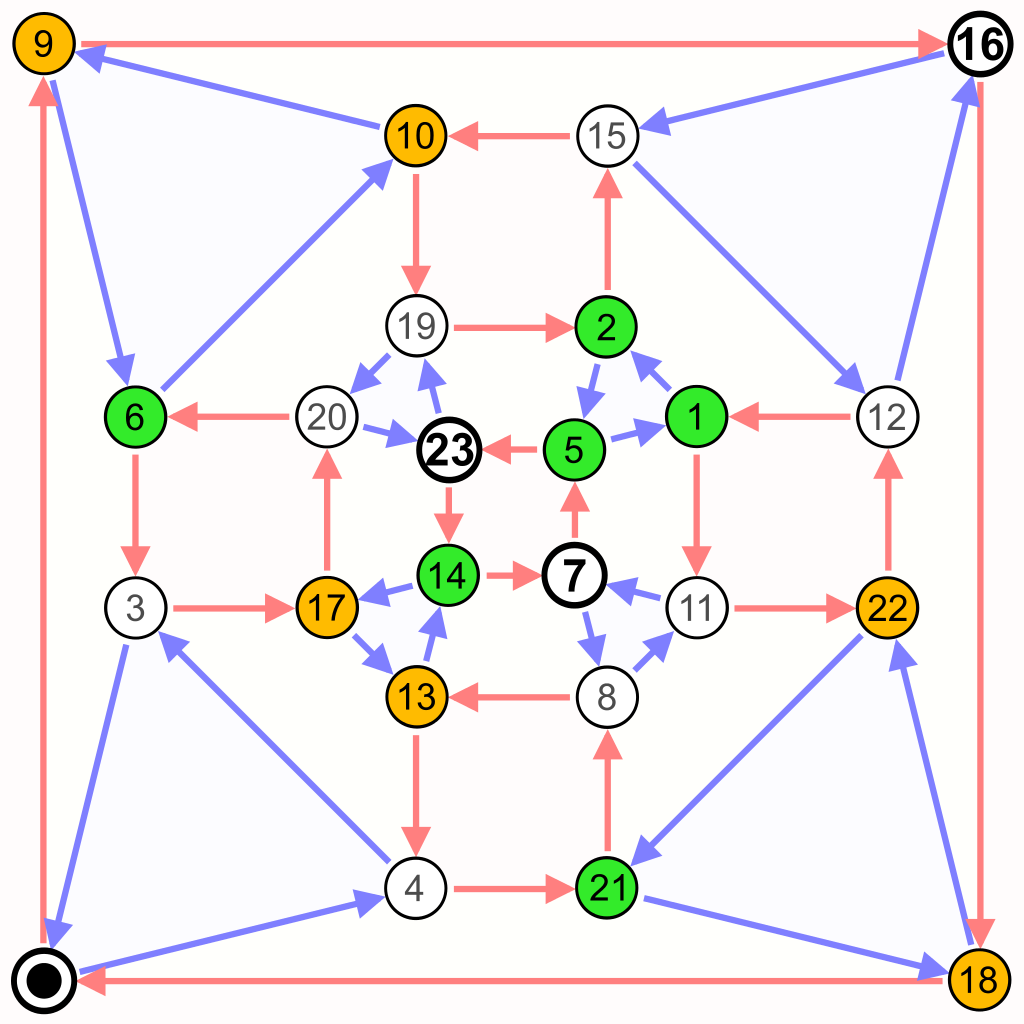
\includegraphics[height=7cm]{numbers.png}
      \caption{Cayley有向图}
      \label{fig:Directed-Cayley-graph}
    \end{minipage}\hfill
    \begin{minipage}{0.48\textwidth}
      \centering
      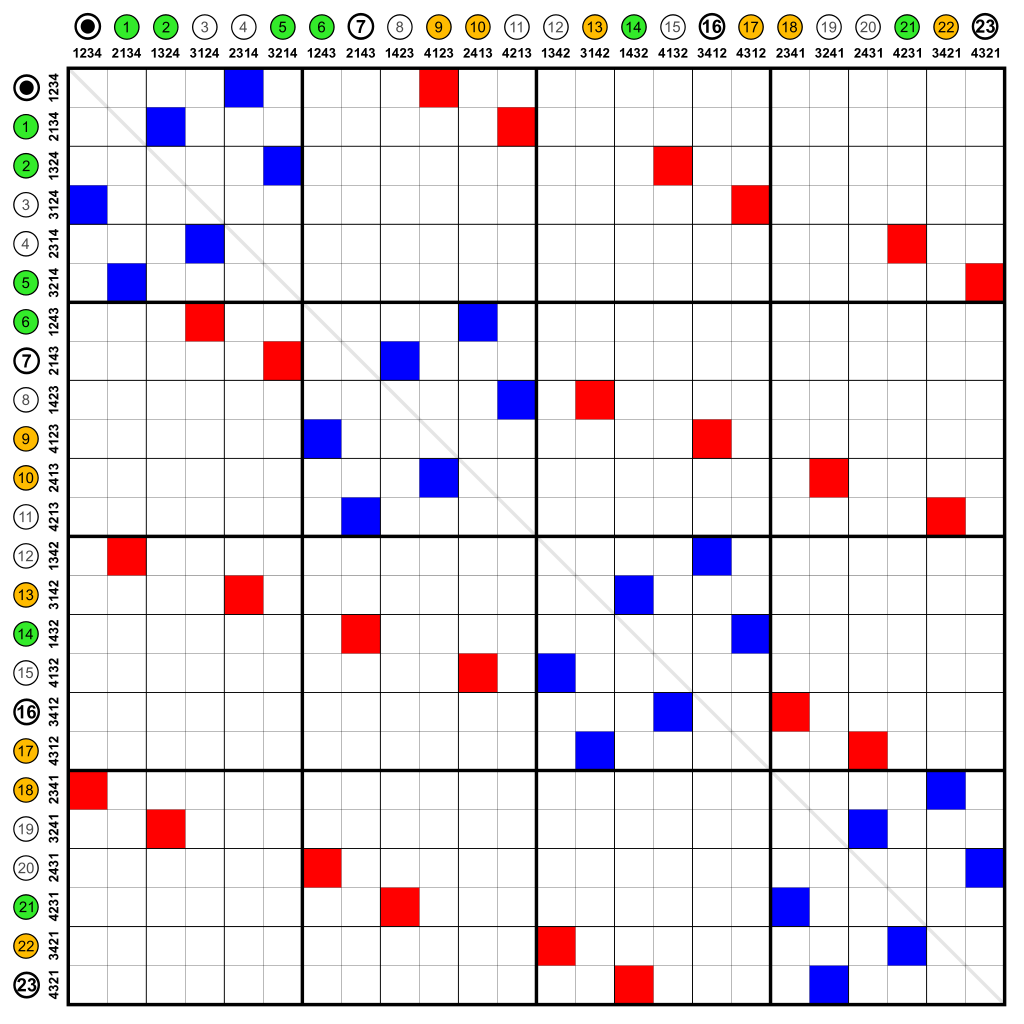
\includegraphics[height=7cm]{adjacency_matrix.png}
      \caption{邻接矩阵}
      \label{fig:Adjacency-matrix}
    \end{minipage}
\end{figure}

我们使用有向图的邻接矩阵A来描述其通信拓扑:

\begin{equation}
    \mathbf{A}=\left[a_{i j}\right]_{N \times N}
\end{equation}

$a_{\mathrm{ij}}$为A中的元素:

\begin{equation}
    a_{\mathrm{ij}}=\left\{\begin{array}{ll}
    {1} & {\text { if } j \in N_{i}} \\
    {0} & {\text { Otherwise }}
    \end{array}\right.
\end{equation}

其中N为与i节点相连通的节点集合。

\begin{equation}
    x_{\mathrm{i}}(t)=x_{\mathrm{i}}(t)+u_{\mathrm{i}}(t) \quad i=1,2,3,4 \ldots \ldots, n
\end{equation}

$u_{\mathrm{i}}(t)$为$x_{\mathrm{i}}(t)$的控制变量,服从:

\begin{equation}
    u_{i}(t)=\frac{1}{N_{\mathrm{i}}}\sum_{j=1}^{n} a_{i j}(t)\left[x_{j}(t)-x_{i}(t)\right]
\end{equation}

其中$N_{\mathrm{i}}$为与i节点相连通的节点数。

上述算法的物理含义即:

在第i次迭代过程中,同时对和每个节点相连通的所有节点取平均并赋值给此节点\cite{8706900}。

用过渡矩阵来说就是:Q阵中每个元素为对应邻接矩阵元素除以此节点出度(发出的边的总数)。

\begin{equation}
    q_{i j}=\frac{a_{i j}}{\sum_{k=1}^{N} a_{i k}}
\end{equation}

但此时收敛速度并非最快,在下一章中将会进行优化。

\subsection{链式通信协议}

对于一个强连通的电网,我们使用有向图的邻接矩阵A来描述其通信拓扑:

\begin{equation}
    \mathbf{A}=\left[a_{i j}\right]_{N \times N}
\end{equation}

\begin{equation}
    a_{i j}=\left\{\begin{array}{l}
    {1} \\
    {0}
    \end{array}\right.
\end{equation}

其中,1表示通信节点j能向i发送消息并被i接收。

\section{算例}

设想一个四节点机组网络有向图如图~\ref{fig:Directed-graph}:

%去除Visio白边:http://www.mamicode.com/info-detail-2181323.html

\begin{figure}[htbp] % use float package if you want it here
    \centering
    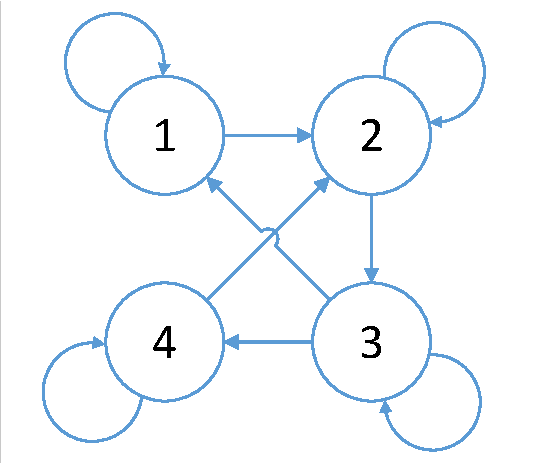
\includegraphics{Directed-graph.pdf}
    \caption{四节点机组网络有向图}
    \label{fig:Directed-graph}
\end{figure}

% 各节点处机组参数与负荷如表~\ref{tab:example}:

% \begin{table}[htbp]
%     \centering
% %    \resizebox{\textwidth}{!}{%
%     \begin{tabular}{@{}ccccc@{}}
%     \toprule
%     \multicolumn{1}{c}{Node} & $\alpha_{i}(\mathrm{MW})$  & $\beta_{i} \quad\left(\mathrm{MW}^{2} / \mathrm{S}\right)$ & $\gamma_{i}(\mathrm{S})$   & $L_{i}(\mathrm{MW})$    \\ \midrule
%     1                        & -1 & 1 & 0.2 & 15.5 \\
%     2                        & -2 & 2 & 0.1 & 0    \\
%     3                        & -3 & 3 & 0.5 & 15.5 \\
%     4                        & -1 & 2 & 0.7 & 0    \\ \bottomrule
%     \end{tabular}
% %    }缩放表格(字会变得很大)
%     \caption{4节点算例机组参数与实时负荷}
%     \label{tab:example}
% \end{table}

其邻接矩阵为:

\begin{equation}
    A=\left[\begin{array}{cccc}
    {1} & {1} & {0} & {0} \\
    {0} & {1} & {1} & {0} \\
    {1} & {0} & {1} & {1} \\
    {0} & {1} & {0} & {1}
    \end{array}\right]
\end{equation}


\section{简化后的平均值共识算法}

% 运行附录~\ref{sec:Consensus}中的Python3脚本我们可以得到:

简单取平均后得到过渡矩阵为

\begin{equation}
    Q=\left[\begin{array}{cccc}
    {\frac{1}{2}} & {\frac{1}{2}} & {0} & {0} \\
    {0} & {\frac{1}{2}} & {\frac{1}{2}} & {0} \\
    {\frac{1}{3}} & {0} & {\frac{1}{3}} & {\frac{1}{3}} \\
    {0} & {\frac{1}{2}} & {0} & {\frac{1}{2}}
    \end{array}\right]
\end{equation}

取初值为1,2,3,4迭代10次:

随着迭代各机组的价格曲线如图~\ref{fig:Result-1234}所示。

\begin{figure}[htbp] % use float package if you want it here
    \centering
    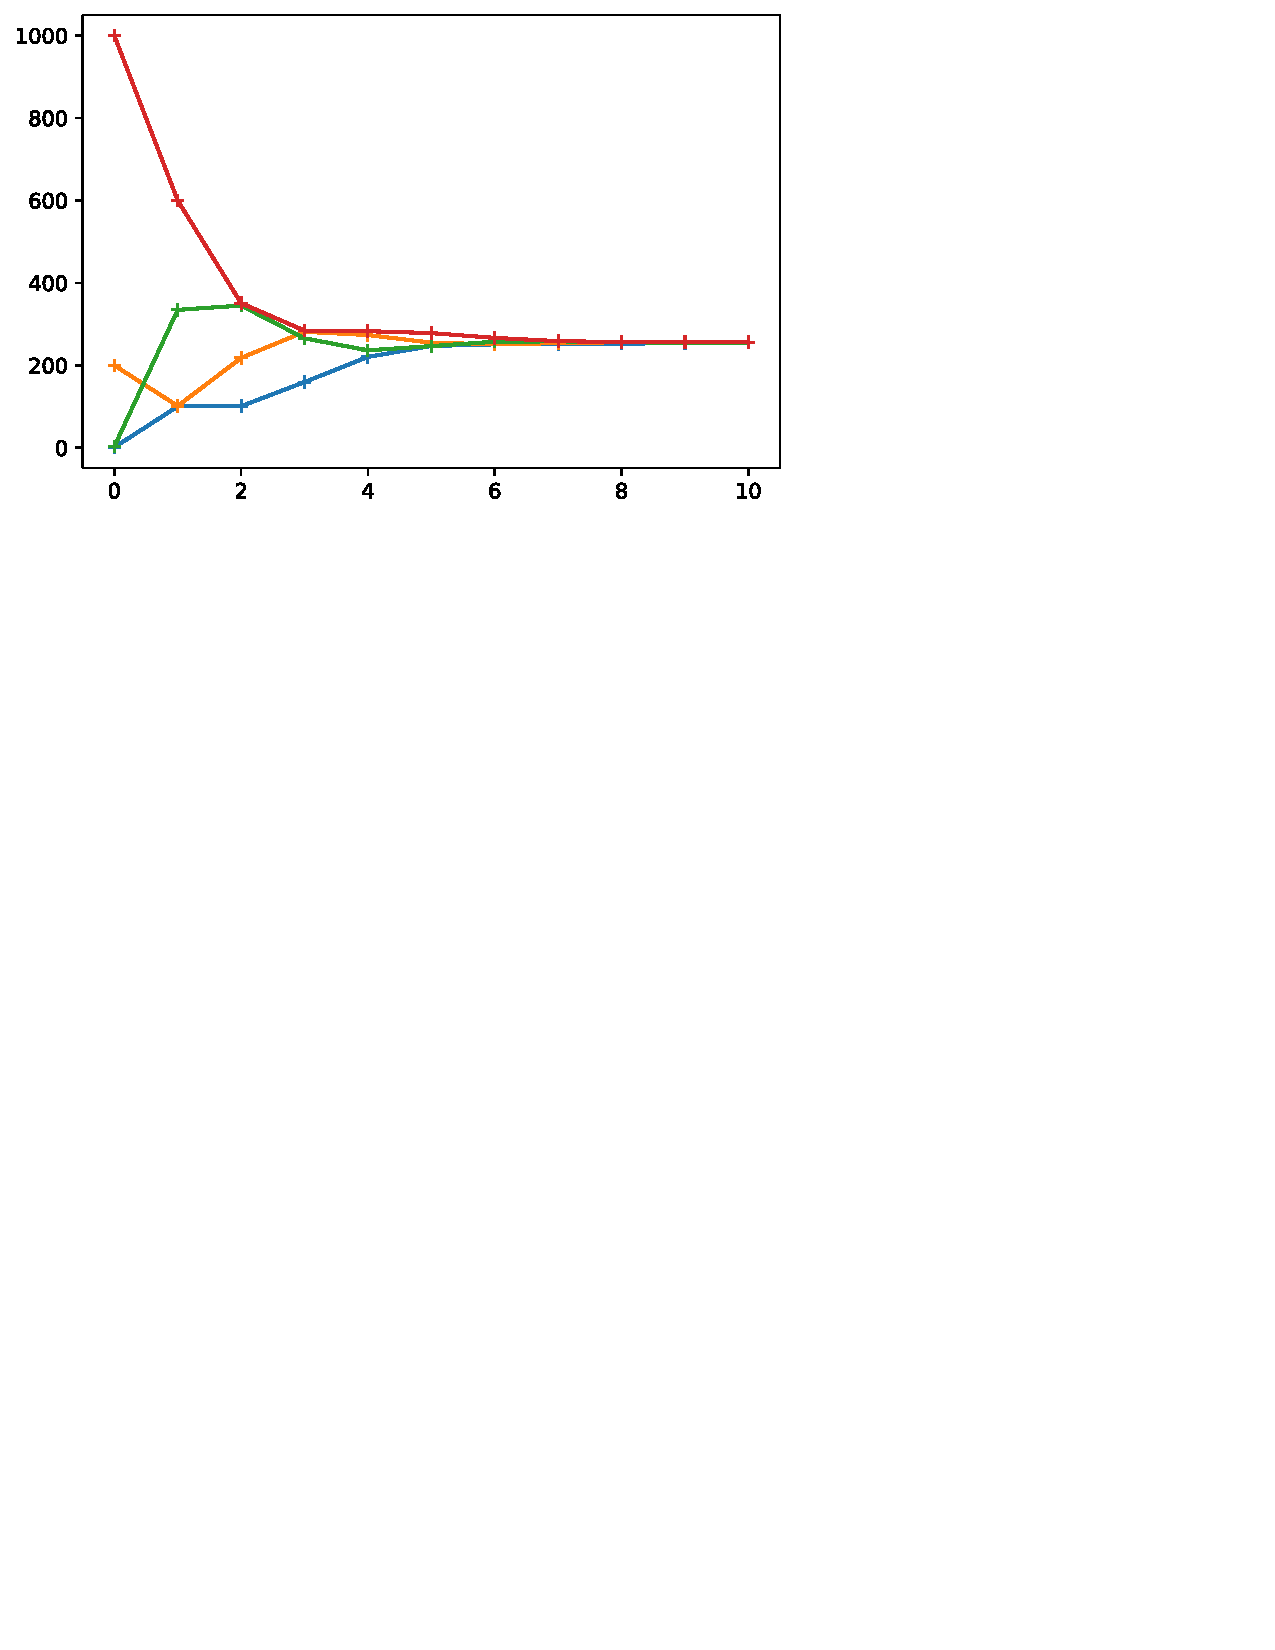
\includegraphics{1234.pdf}
    \caption{初值为1,2,3,4迭代10次的价格曲线}
    \label{fig:Result-1234}
\end{figure}

数据如表~\ref{tab:Result-1234}所示。

\begin{table}[htbp]
    \centering
    \begin{tabular}{|l|l|l|l|l|}
    \hline
    \diagbox{迭代次数}{$X_{i,j}$}{节点编号} %添加斜线表头
       & 0        & 1        & 2        & 3        \\ \hline
    0  & 1        & 2        & 3        & 4        \\ \hline
    1  & 1.5      & 2.5      & 2.666667 & 3        \\ \hline
    2  & 2        & 2.583333 & 2.388889 & 2.75     \\ \hline
    3  & 2.291667 & 2.486111 & 2.37963  & 2.666667 \\ \hline
    4  & 2.388889 & 2.43287  & 2.445988 & 2.576389 \\ \hline
    5  & 2.41088  & 2.439429 & 2.470422 & 2.50463  \\ \hline
    6  & 2.425154 & 2.454925 & 2.461977 & 2.472029 \\ \hline
    7  & 2.44004  & 2.458451 & 2.453054 & 2.463477 \\ \hline
    8  & 2.449246 & 2.455752 & 2.45219  & 2.460964 \\ \hline
    9  & 2.452499 & 2.453971 & 2.454133 & 2.458358 \\ \hline
    10 & 2.453235 & 2.454052 & 2.454997 & 2.456165 \\ \hline
    \end{tabular}
    \caption{初值为1,2,3,4迭代10次各节点价格变化}
    \label{tab:Result-1234}
\end{table}

取初值为1000,0,0,0迭代10次:

随着迭代各机组的价格曲线如图~\ref{fig:Result-1000}所示。

\begin{figure}[htbp] % use float package if you want it here
    \centering
    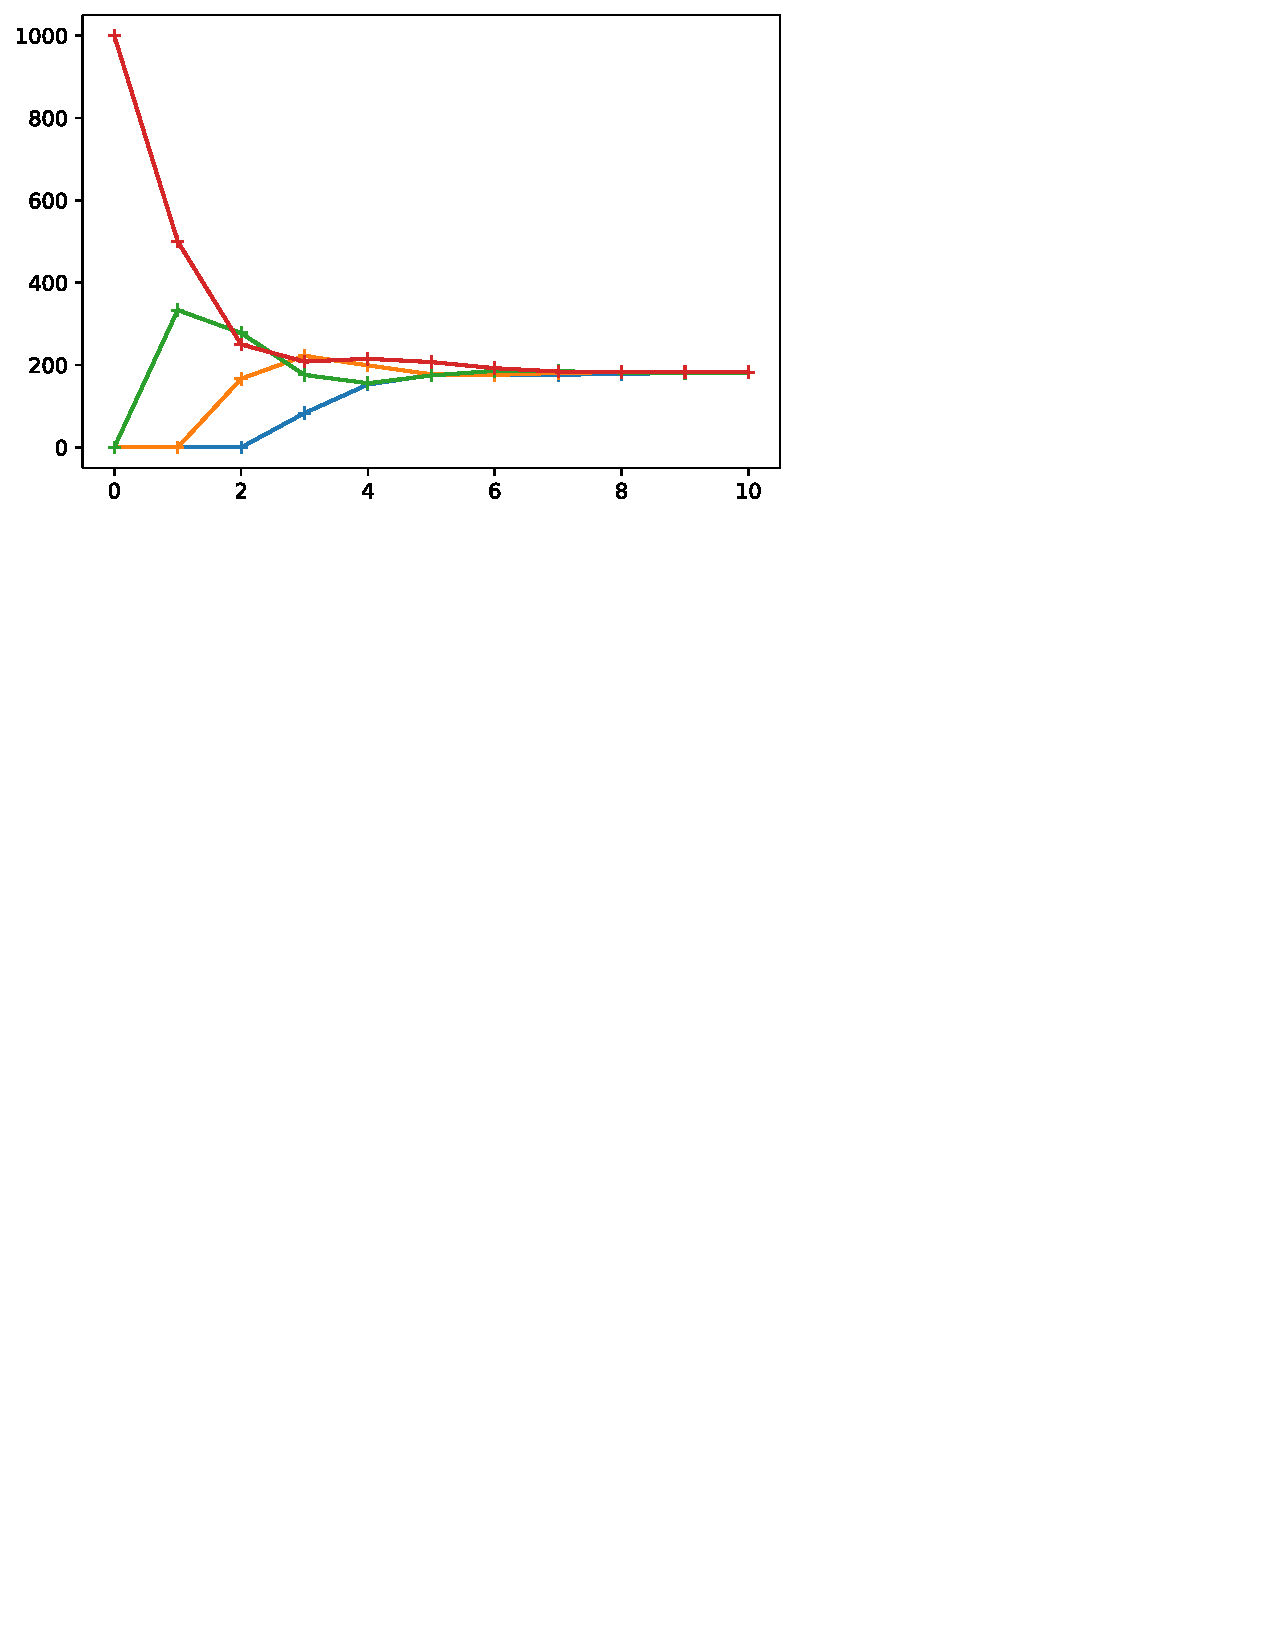
\includegraphics{1000.pdf}
    \caption{初值为1000,0,0,0迭代10次的价格曲线}
    \label{fig:Result-1000}
\end{figure}

数据如表~\ref{tab:Result-1000}所示。

\begin{table}[htbp]
    \centering
    \begin{tabular}{|l|l|l|l|l|}
    \hline
    \diagbox{迭代次数}{$X_{i,j}$}{节点编号} %添加斜线表头
       & 0        & 1        & 2        & 3        \\ \hline
    0  & 0        & 0        & 0        & 1000     \\ \hline
    1  & 0        & 0        & 333.3333 & 500      \\ \hline
    2  & 0        & 166.6667 & 277.7778 & 250      \\ \hline
    3  & 83.33333 & 222.2222 & 175.9259 & 208.3333 \\ \hline
    4  & 152.7778 & 199.0741 & 155.8642 & 215.2778 \\ \hline
    5  & 175.9259 & 177.4691 & 174.6399 & 207.1759 \\ \hline
    6  & 176.6975 & 176.0545 & 185.9139 & 192.3225 \\ \hline
    7  & 176.376  & 180.9842 & 184.978  & 184.1885 \\ \hline
    8  & 178.6801 & 182.9811 & 181.8475 & 182.5864 \\ \hline
    9  & 180.8306 & 182.4143 & 181.038  & 182.7837 \\ \hline
    10 & 181.6225 & 181.7262 & 181.5508 & 182.599  \\ \hline
    \end{tabular}
    \caption{初值为1000,0,0,0迭代10次各节点价格变化}
    \label{tab:Result-1000}
\end{table}

\section{非强连通图反例}

对于一个非强连通图,有向图中的强连通分量会因为单向连接的节点产生全局性的错误迭代结果,需要时刻保证剔除通信错误节点,可以使用握手协议的方法保障双向通信的可靠性。

例如一个10节点系统,1-10号节点取值分别对应为1-10,邻接矩阵A如表~\ref{tab:Error-A}所示。

\begin{table}[htbp]
    \centering
    \begin{tabular}{|l|l|l|l|l|l|l|l|l|l|l|}
    \hline
    \diagbox{i节点编号}{$A_{i,j}$}{j节点编号} %添加斜线表头
       & 1 & 2 & 3 & 4 & 5 & 6 & 7 & 8 & 9 & 10 \\ \hline
    1  & 1 & 1 & 0 & 0 & 1 & 1 & 0 & 1 & 0 & 0  \\ \hline
    2  & 0 & 1 & 1 & 0 & 0 & 0 & 1 & 0 & 1 & 0  \\ \hline
    3  & 1 & 0 & 1 & 1 & 0 & 0 & 1 & 1 & 0 & 1  \\ \hline
    4  & 0 & 1 & 0 & 1 & 0 & 1 & 0 & 0 & 1 & 0  \\ \hline
    5  & 0 & 0 & 0 & 0 & 1 & 0 & 0 & 0 & 0 & 1  \\ \hline
    6  & 0 & 0 & 0 & 0 & 0 & 1 & 0 & 1 & 0 & 0  \\ \hline
    7  & 0 & 0 & 0 & 0 & 0 & 0 & 1 & 0 & 0 & 1  \\ \hline
    8  & 0 & 1 & 0 & 0 & 1 & 1 & 0 & 0 & 0 & 0  \\ \hline
    9  & 0 & 0 & 0 & 0 & 0 & 0 & 0 & 0 & 1 & 0  \\ \hline
    10 & 0 & 0 & 0 & 0 & 1 & 0 & 1 & 0 & 1 & 1  \\ \hline
    \end{tabular}
    \caption{非强连通图反例A矩阵}
    \label{tab:Error-A}
\end{table}

注意表~\ref{tab:Error-A}中9号节点没有办法接收到其他节点的信息,成为了和其他节点分立的强连通分量,$A_{9,9}=1$是指9号节点能接受到自己的信息,9号节点因此成为错误节点,如果不加握手验证的话,9号节点就成为了害群之马,使得整个网络错误的收敛到9号节点的值9上,而非正确的5.5。

迭代20次曲线如图~\ref{fig:123456-Error}所示。

\begin{figure}[htbp]
    \centering
    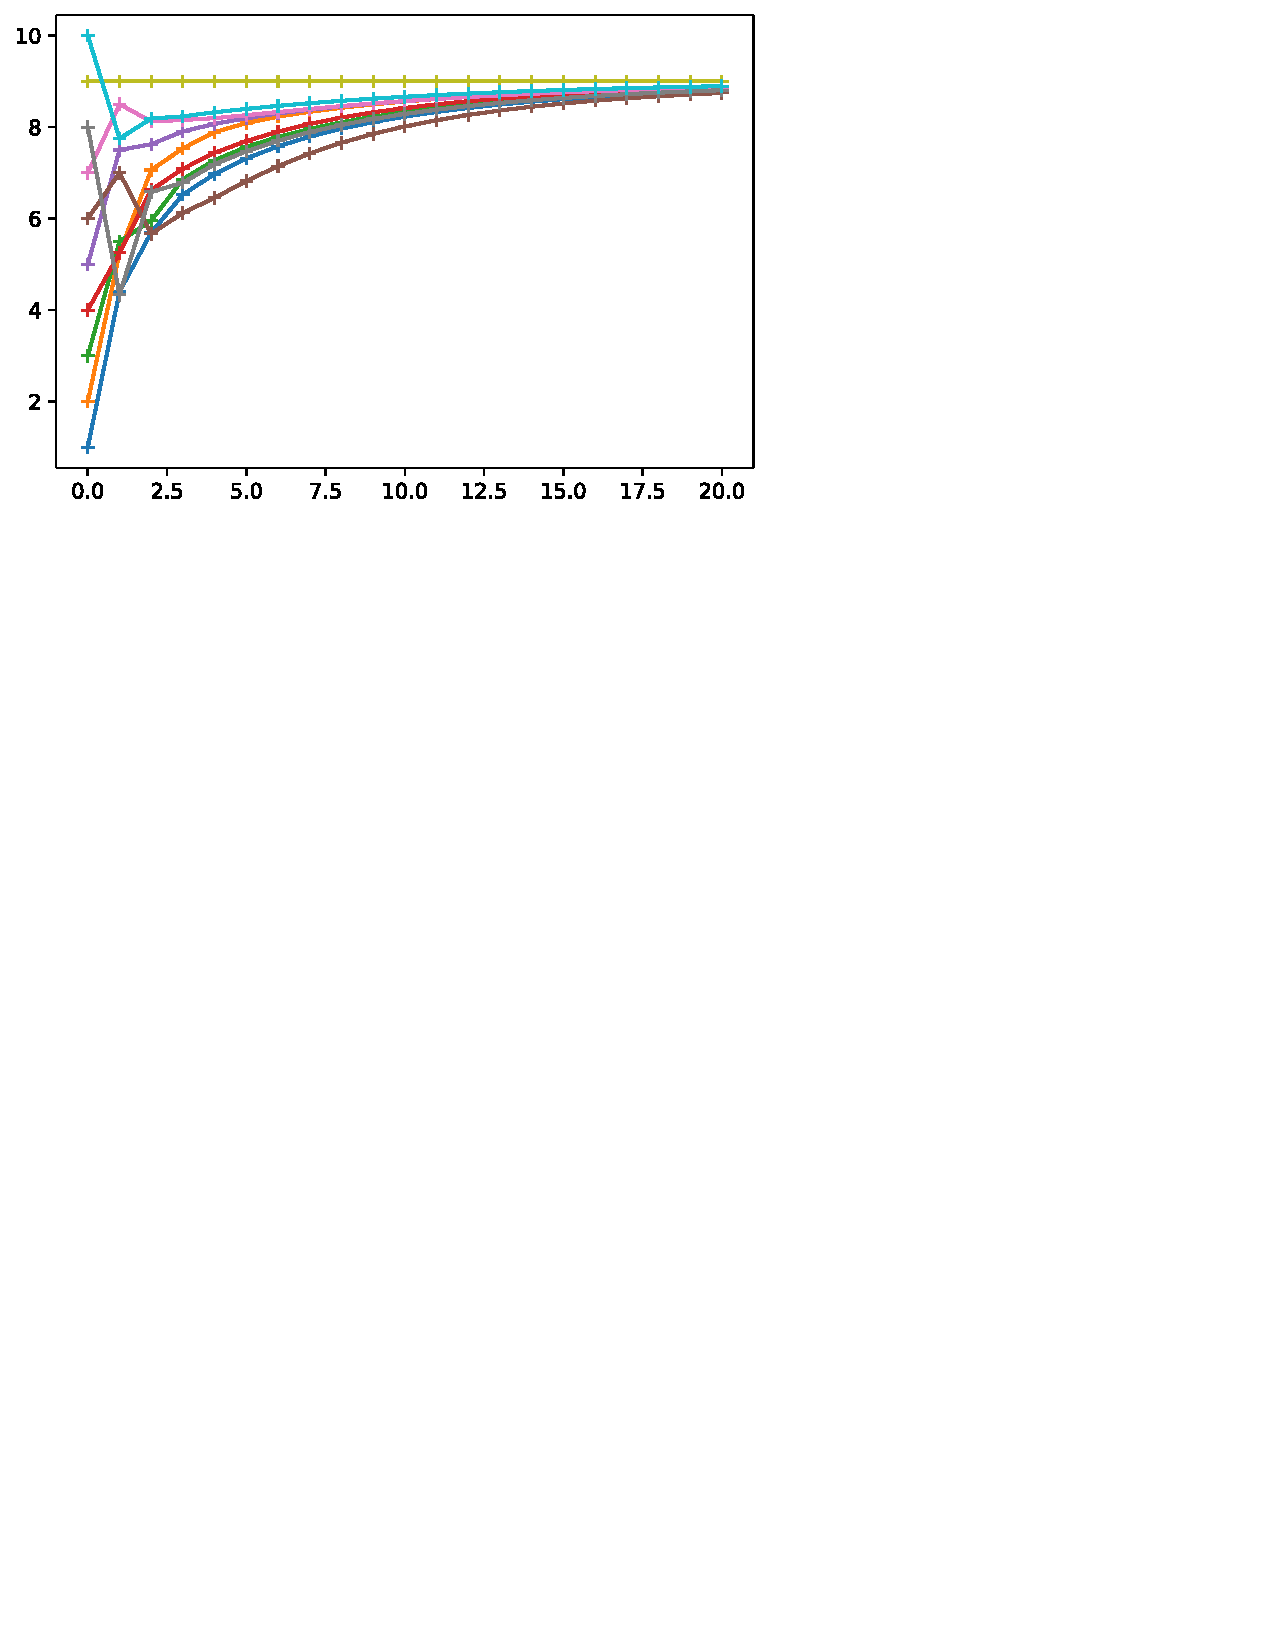
\includegraphics{123456-Error.pdf}
    \caption{非强连通图反例迭代曲线}
    \label{fig:123456-Error}
\end{figure}

数据如表~\ref{tab:123456-Error}所示。

\begin{table}[htbp]
    \centering
    \begin{tabular}{|l|l|l|l|l|l|l|l|l|l|l|}
    \hline
    \diagbox{迭代次数}{$Y_{i,j}$}{节点编号} %添加斜线表头
       & 1    & 2    & 3    & 4    & 5    & 6    & 7    & 8    & 9    & 10    \\ \hline
    0  & 1.00 & 2.00 & 3.00 & 4.00 & 5.00 & 6.00 & 7.00 & 8.00 & 9.00 & 10.00 \\ \hline
    1  & 4.40 & 5.25 & 5.50 & 5.25 & 7.50 & 7.00 & 8.50 & 4.33 & 9.00 & 7.75  \\ \hline
    2  & 5.70 & 7.06 & 5.96 & 6.63 & 7.63 & 5.67 & 8.13 & 6.58 & 9.00 & 8.19  \\ \hline
    3  & 6.53 & 7.54 & 6.86 & 7.09 & 7.91 & 6.13 & 8.16 & 6.78 & 9.00 & 8.23  \\ \hline
    4  & 6.98 & 7.89 & 7.28 & 7.44 & 8.07 & 6.45 & 8.20 & 7.19 & 9.00 & 8.32  \\ \hline
    5  & 7.32 & 8.09 & 7.57 & 7.70 & 8.20 & 6.82 & 8.26 & 7.47 & 9.00 & 8.40  \\ \hline
    6  & 7.58 & 8.23 & 7.78 & 7.90 & 8.30 & 7.15 & 8.33 & 7.70 & 9.00 & 8.46  \\ \hline
    7  & 7.79 & 8.34 & 7.96 & 8.07 & 8.38 & 7.42 & 8.40 & 7.89 & 9.00 & 8.52  \\ \hline
    8  & 7.96 & 8.42 & 8.10 & 8.21 & 8.45 & 7.66 & 8.46 & 8.05 & 9.00 & 8.57  \\ \hline
    9  & 8.11 & 8.50 & 8.23 & 8.32 & 8.51 & 7.85 & 8.52 & 8.18 & 9.00 & 8.62  \\ \hline
    10 & 8.23 & 8.56 & 8.33 & 8.42 & 8.57 & 8.01 & 8.57 & 8.29 & 9.00 & 8.66  \\ \hline
    11 & 8.33 & 8.61 & 8.42 & 8.50 & 8.62 & 8.15 & 8.62 & 8.38 & 9.00 & 8.70  \\ \hline
    12 & 8.42 & 8.66 & 8.49 & 8.57 & 8.66 & 8.27 & 8.66 & 8.46 & 9.00 & 8.73  \\ \hline
    13 & 8.49 & 8.70 & 8.55 & 8.62 & 8.70 & 8.36 & 8.70 & 8.53 & 9.00 & 8.76  \\ \hline
    14 & 8.56 & 8.74 & 8.61 & 8.67 & 8.73 & 8.45 & 8.73 & 8.59 & 9.00 & 8.79  \\ \hline
    15 & 8.61 & 8.77 & 8.66 & 8.71 & 8.76 & 8.52 & 8.76 & 8.64 & 9.00 & 8.81  \\ \hline
    16 & 8.66 & 8.80 & 8.70 & 8.75 & 8.78 & 8.58 & 8.78 & 8.68 & 9.00 & 8.83  \\ \hline
    17 & 8.70 & 8.82 & 8.73 & 8.78 & 8.81 & 8.63 & 8.81 & 8.72 & 9.00 & 8.85  \\ \hline
    18 & 8.74 & 8.84 & 8.77 & 8.81 & 8.83 & 8.67 & 8.83 & 8.75 & 9.00 & 8.87  \\ \hline
    19 & 8.77 & 8.86 & 8.79 & 8.83 & 8.85 & 8.71 & 8.85 & 8.78 & 9.00 & 8.88  \\ \hline
    20 & 8.79 & 8.87 & 8.82 & 8.85 & 8.86 & 8.75 & 8.86 & 8.81 & 9.00 & 8.89  \\ \hline
    \end{tabular}
    \caption{非强连通图反例迭代数据}
    \label{tab:123456-Error}
\end{table}


将其他任意$A_{9,j}$改为1后,就可以变成强连通系统,正常收敛。例如将从节点9到1的有向边连接起来,即令$A_{9,1}=1$其他不变,邻接矩阵A变为如表~\ref{tab:Correct-A}所示。

\begin{table}[htbp]
    \centering
    \begin{tabular}{|l|l|l|l|l|l|l|l|l|l|l|}
    \hline
    \diagbox{i节点编号}{$A_{i,j}$}{j节点编号} %添加斜线表头
       & 1 & 2 & 3 & 4 & 5 & 6 & 7 & 8 & 9 & 10 \\ \hline
    1  & 1 & 1 & 0 & 0 & 1 & 1 & 0 & 1 & 0 & 0  \\ \hline
    2  & 0 & 1 & 1 & 0 & 0 & 0 & 1 & 0 & 1 & 0  \\ \hline
    3  & 1 & 0 & 1 & 1 & 0 & 0 & 1 & 1 & 0 & 1  \\ \hline
    4  & 0 & 1 & 0 & 1 & 0 & 1 & 0 & 0 & 1 & 0  \\ \hline
    5  & 0 & 0 & 0 & 0 & 1 & 0 & 0 & 0 & 0 & 1  \\ \hline
    6  & 0 & 0 & 0 & 0 & 0 & 1 & 0 & 1 & 0 & 0  \\ \hline
    7  & 0 & 0 & 0 & 0 & 0 & 0 & 1 & 0 & 0 & 1  \\ \hline
    8  & 0 & 1 & 0 & 0 & 1 & 1 & 0 & 0 & 0 & 0  \\ \hline
    9  & 1 & 0 & 0 & 0 & 0 & 0 & 0 & 0 & 1 & 0  \\ \hline
    10 & 0 & 0 & 0 & 0 & 1 & 0 & 1 & 0 & 1 & 1  \\ \hline
    \end{tabular}
    \caption{纠正后的强连通图A矩阵}
    \label{tab:Correct-A}
\end{table}

迭代20次曲线如图~\ref{fig:123456-Correct}所示。

\begin{figure}[htbp]
    \centering
    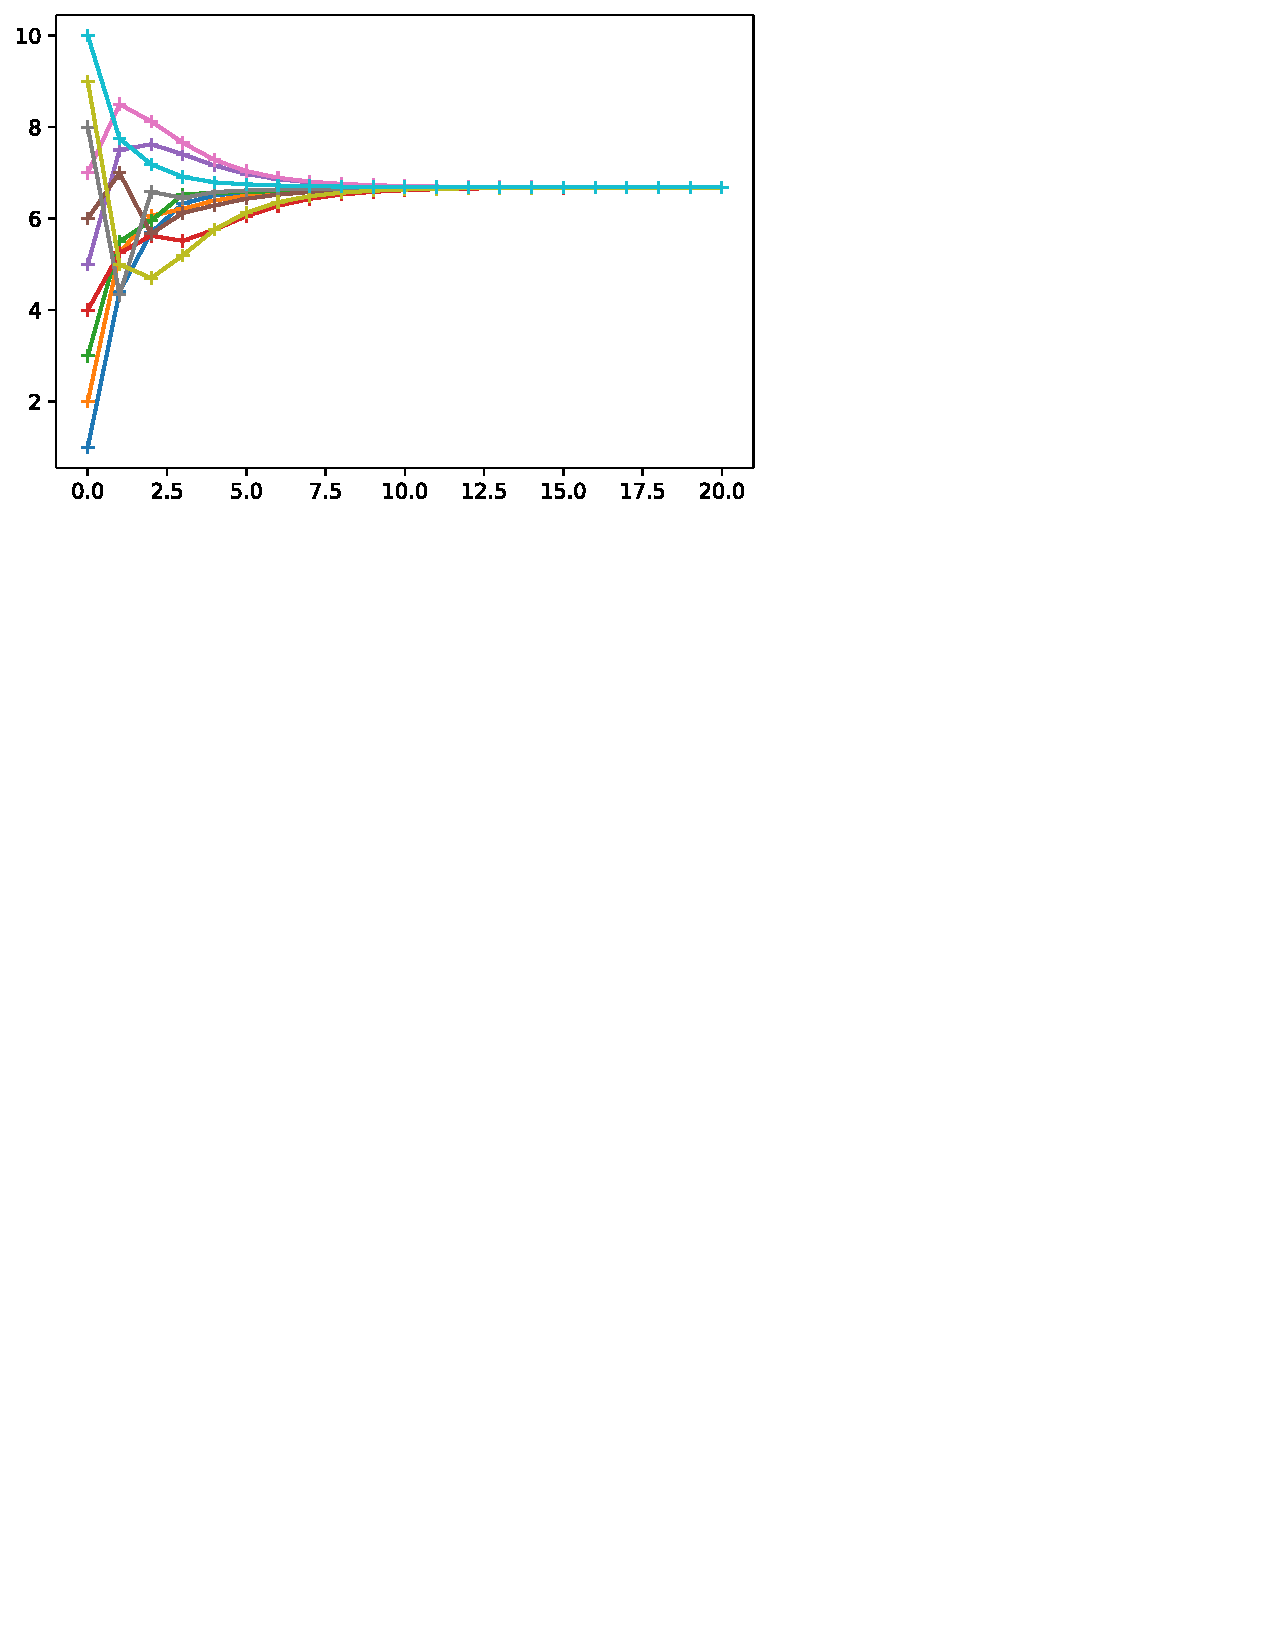
\includegraphics{123456-Correct.pdf}
    \caption{纠正后的强连通图迭代曲线}
    \label{fig:123456-Correct}
\end{figure}

数据如表~\ref{tab:123456-Correct}所示。

\begin{table}[htbp]
    \centering
    \begin{tabular}{|l|l|l|l|l|l|l|l|l|l|l|}
    \hline
    \diagbox{迭代次数}{$Y_{i,j}$}{节点编号} %添加斜线表头
       & 0    & 1    & 2    & 3    & 4    & 5    & 6    & 7    & 8    & 9     \\ \hline
    0  & 1.00 & 2.00 & 3.00 & 4.00 & 5.00 & 6.00 & 7.00 & 8.00 & 9.00 & 10.00 \\ \hline
    1  & 4.40 & 5.25 & 5.50 & 5.25 & 7.50 & 7.00 & 8.50 & 4.33 & 5.00 & 7.75  \\ \hline
    2  & 5.70 & 6.06 & 5.96 & 5.63 & 7.63 & 5.67 & 8.13 & 6.58 & 4.70 & 7.19  \\ \hline
    3  & 6.33 & 6.21 & 6.53 & 5.51 & 7.41 & 6.13 & 7.66 & 6.45 & 5.20 & 6.91  \\ \hline
    4  & 6.50 & 6.40 & 6.56 & 5.76 & 7.16 & 6.29 & 7.28 & 6.58 & 5.76 & 6.79  \\ \hline
    5  & 6.59 & 6.50 & 6.58 & 6.05 & 6.98 & 6.43 & 7.04 & 6.61 & 6.13 & 6.75  \\ \hline
    6  & 6.62 & 6.56 & 6.60 & 6.28 & 6.86 & 6.52 & 6.89 & 6.64 & 6.36 & 6.72  \\ \hline
    7  & 6.64 & 6.60 & 6.63 & 6.43 & 6.79 & 6.58 & 6.81 & 6.65 & 6.49 & 6.71  \\ \hline
    8  & 6.65 & 6.63 & 6.64 & 6.53 & 6.75 & 6.62 & 6.76 & 6.66 & 6.57 & 6.70  \\ \hline
    9  & 6.66 & 6.65 & 6.66 & 6.59 & 6.73 & 6.64 & 6.73 & 6.67 & 6.61 & 6.69  \\ \hline
    10 & 6.67 & 6.66 & 6.67 & 6.62 & 6.71 & 6.65 & 6.71 & 6.67 & 6.64 & 6.69  \\ \hline
    11 & 6.67 & 6.67 & 6.67 & 6.64 & 6.70 & 6.66 & 6.70 & 6.67 & 6.65 & 6.69  \\ \hline
    12 & 6.68 & 6.67 & 6.68 & 6.66 & 6.69 & 6.67 & 6.69 & 6.68 & 6.66 & 6.69  \\ \hline
    13 & 6.68 & 6.68 & 6.68 & 6.67 & 6.69 & 6.67 & 6.69 & 6.68 & 6.67 & 6.68  \\ \hline
    14 & 6.68 & 6.68 & 6.68 & 6.67 & 6.69 & 6.68 & 6.69 & 6.68 & 6.67 & 6.68  \\ \hline
    15 & 6.68 & 6.68 & 6.68 & 6.67 & 6.68 & 6.68 & 6.68 & 6.68 & 6.68 & 6.68  \\ \hline
    16 & 6.68 & 6.68 & 6.68 & 6.68 & 6.68 & 6.68 & 6.68 & 6.68 & 6.68 & 6.68  \\ \hline
    17 & 6.68 & 6.68 & 6.68 & 6.68 & 6.68 & 6.68 & 6.68 & 6.68 & 6.68 & 6.68  \\ \hline
    18 & 6.68 & 6.68 & 6.68 & 6.68 & 6.68 & 6.68 & 6.68 & 6.68 & 6.68 & 6.68  \\ \hline
    19 & 6.68 & 6.68 & 6.68 & 6.68 & 6.68 & 6.68 & 6.68 & 6.68 & 6.68 & 6.68  \\ \hline
    20 & 6.68 & 6.68 & 6.68 & 6.68 & 6.68 & 6.68 & 6.68 & 6.68 & 6.68 & 6.68  \\ \hline
    \end{tabular}
    \caption{纠正后的强连通图迭代数据}
    \label{tab:123456-Correct}
\end{table}


\section{有新节点加入的算例}

整个四节点系统邻接矩阵为:

\begin{equation}
    A=\left[\begin{array}{cccc}
    {1} & {1} & {0} & {0} \\
    {0} & {1} & {1} & {0} \\
    {1} & {0} & {1} & {1} \\
    {0} & {1} & {0} & {1}
    \end{array}\right]
\end{equation}

初始3节点系统迭代10次曲线如图~\ref{fig:123}所示。

\begin{figure}[htbp]
    \centering
    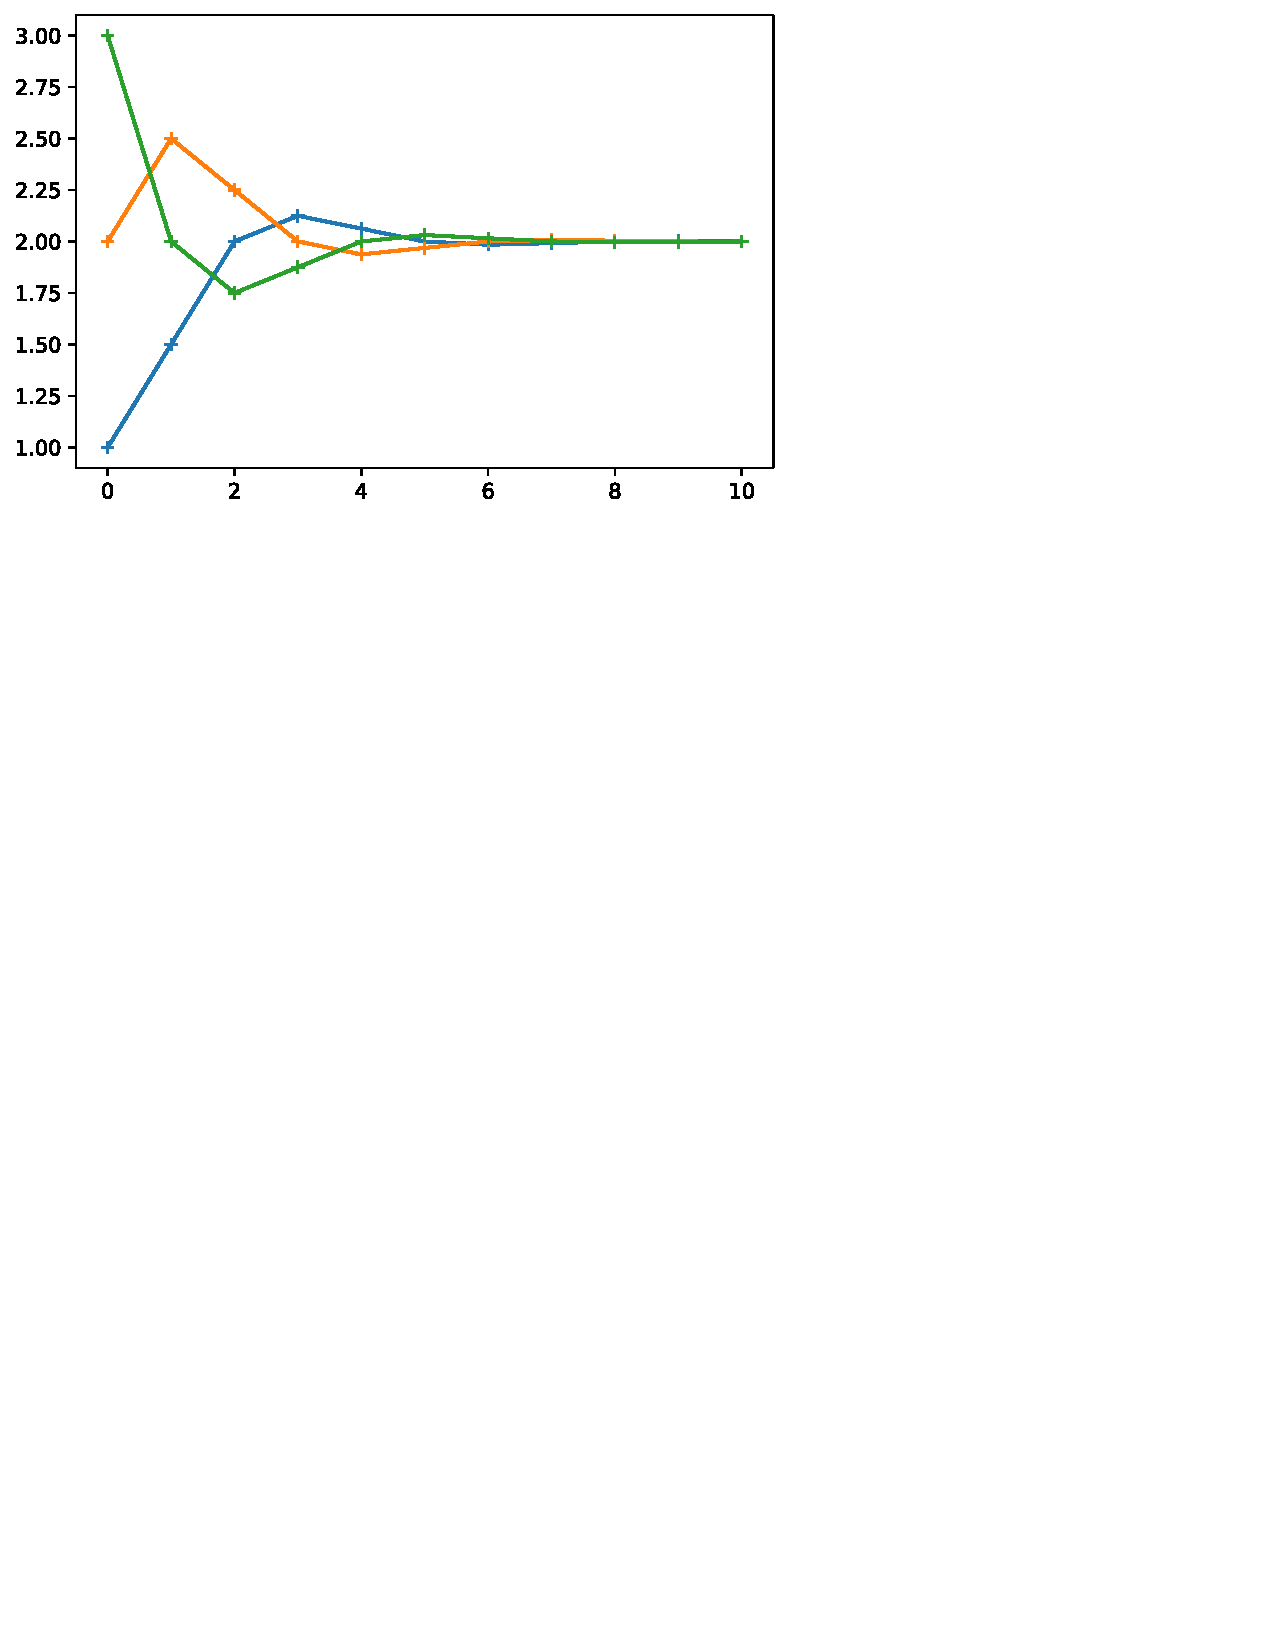
\includegraphics{123.pdf}
    \caption{初始3节点系统迭代10次}
    \label{fig:123}
\end{figure}

数据如表~\ref{tab:123}所示。

\begin{table}[htbp]
    \centering
    \begin{tabular}{|l|l|l|l|}
    \hline
    \diagbox{迭代次数}{$Y_{i,j}$}{节点编号} %添加斜线表头
       & 1    & 2    & 3    \\ \hline
    0  & 1.00 & 2.00 & 3.00 \\ \hline
    1  & 1.50 & 2.50 & 2.00 \\ \hline
    2  & 2.00 & 2.25 & 1.75 \\ \hline
    3  & 2.13 & 2.00 & 1.88 \\ \hline
    4  & 2.06 & 1.94 & 2.00 \\ \hline
    5  & 2.00 & 1.97 & 2.03 \\ \hline
    6  & 1.98 & 2.00 & 2.02 \\ \hline
    7  & 1.99 & 2.01 & 2.00 \\ \hline
    8  & 2.00 & 2.00 & 2.00 \\ \hline
    9  & 2.00 & 2.00 & 2.00 \\ \hline
    10 & 2.00 & 2.00 & 2.00 \\ \hline
    \end{tabular}
    \caption{初始3节点系统迭代过程}
    \label{tab:123}
\end{table}

稳态后加入新节点迭代10次曲线如图~\ref{fig:2224}所示。

\begin{figure}[htbp]
    \centering
    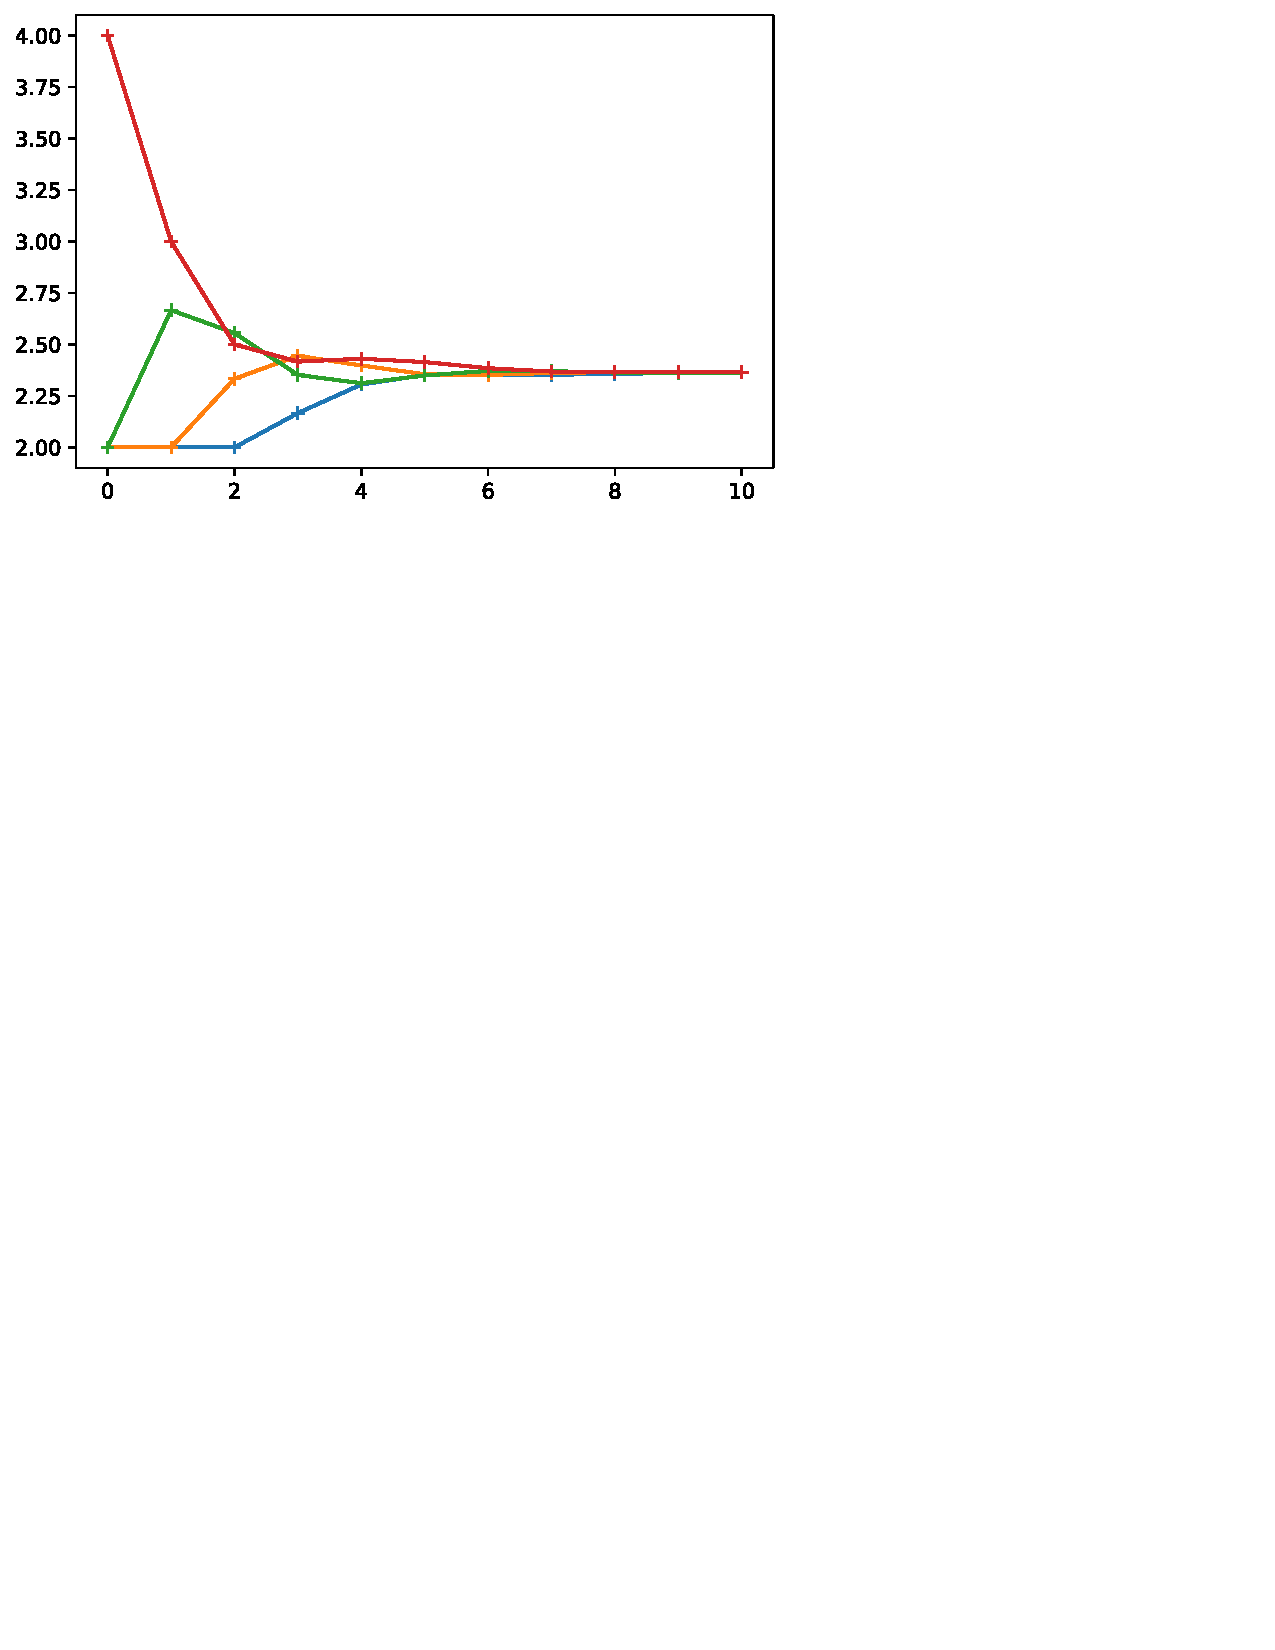
\includegraphics{2224.pdf}
    \caption{稳态后加入新节点迭代10次曲线}
    \label{fig:2224}
\end{figure}

数据如表~\ref{tab:2224}所示。

\begin{table}[htbp]
    \centering
    \begin{tabular}{|l|l|l|l|l|}
    \hline
    \diagbox{迭代次数}{$Y_{i,j}$}{节点编号} %添加斜线表头
       & 1    & 2    & 3    & 4    \\ \hline
    0  & 2.00 & 2.00 & 2.00 & 4.00 \\ \hline
    1  & 2.00 & 2.00 & 2.67 & 3.00 \\ \hline
    2  & 2.00 & 2.33 & 2.56 & 2.50 \\ \hline
    3  & 2.17 & 2.44 & 2.35 & 2.42 \\ \hline
    4  & 2.31 & 2.40 & 2.31 & 2.43 \\ \hline
    5  & 2.35 & 2.35 & 2.35 & 2.41 \\ \hline
    6  & 2.35 & 2.35 & 2.37 & 2.38 \\ \hline
    7  & 2.35 & 2.36 & 2.37 & 2.37 \\ \hline
    8  & 2.36 & 2.37 & 2.36 & 2.37 \\ \hline
    9  & 2.36 & 2.36 & 2.36 & 2.37 \\ \hline
    10 & 2.36 & 2.36 & 2.36 & 2.37 \\ \hline
    \end{tabular}
    \caption{稳态后加入新节点}
    \label{tab:2224}
\end{table}

整个过程如图~\ref{fig:123-2224}所示。

\begin{figure}[htbp]
    \centering
    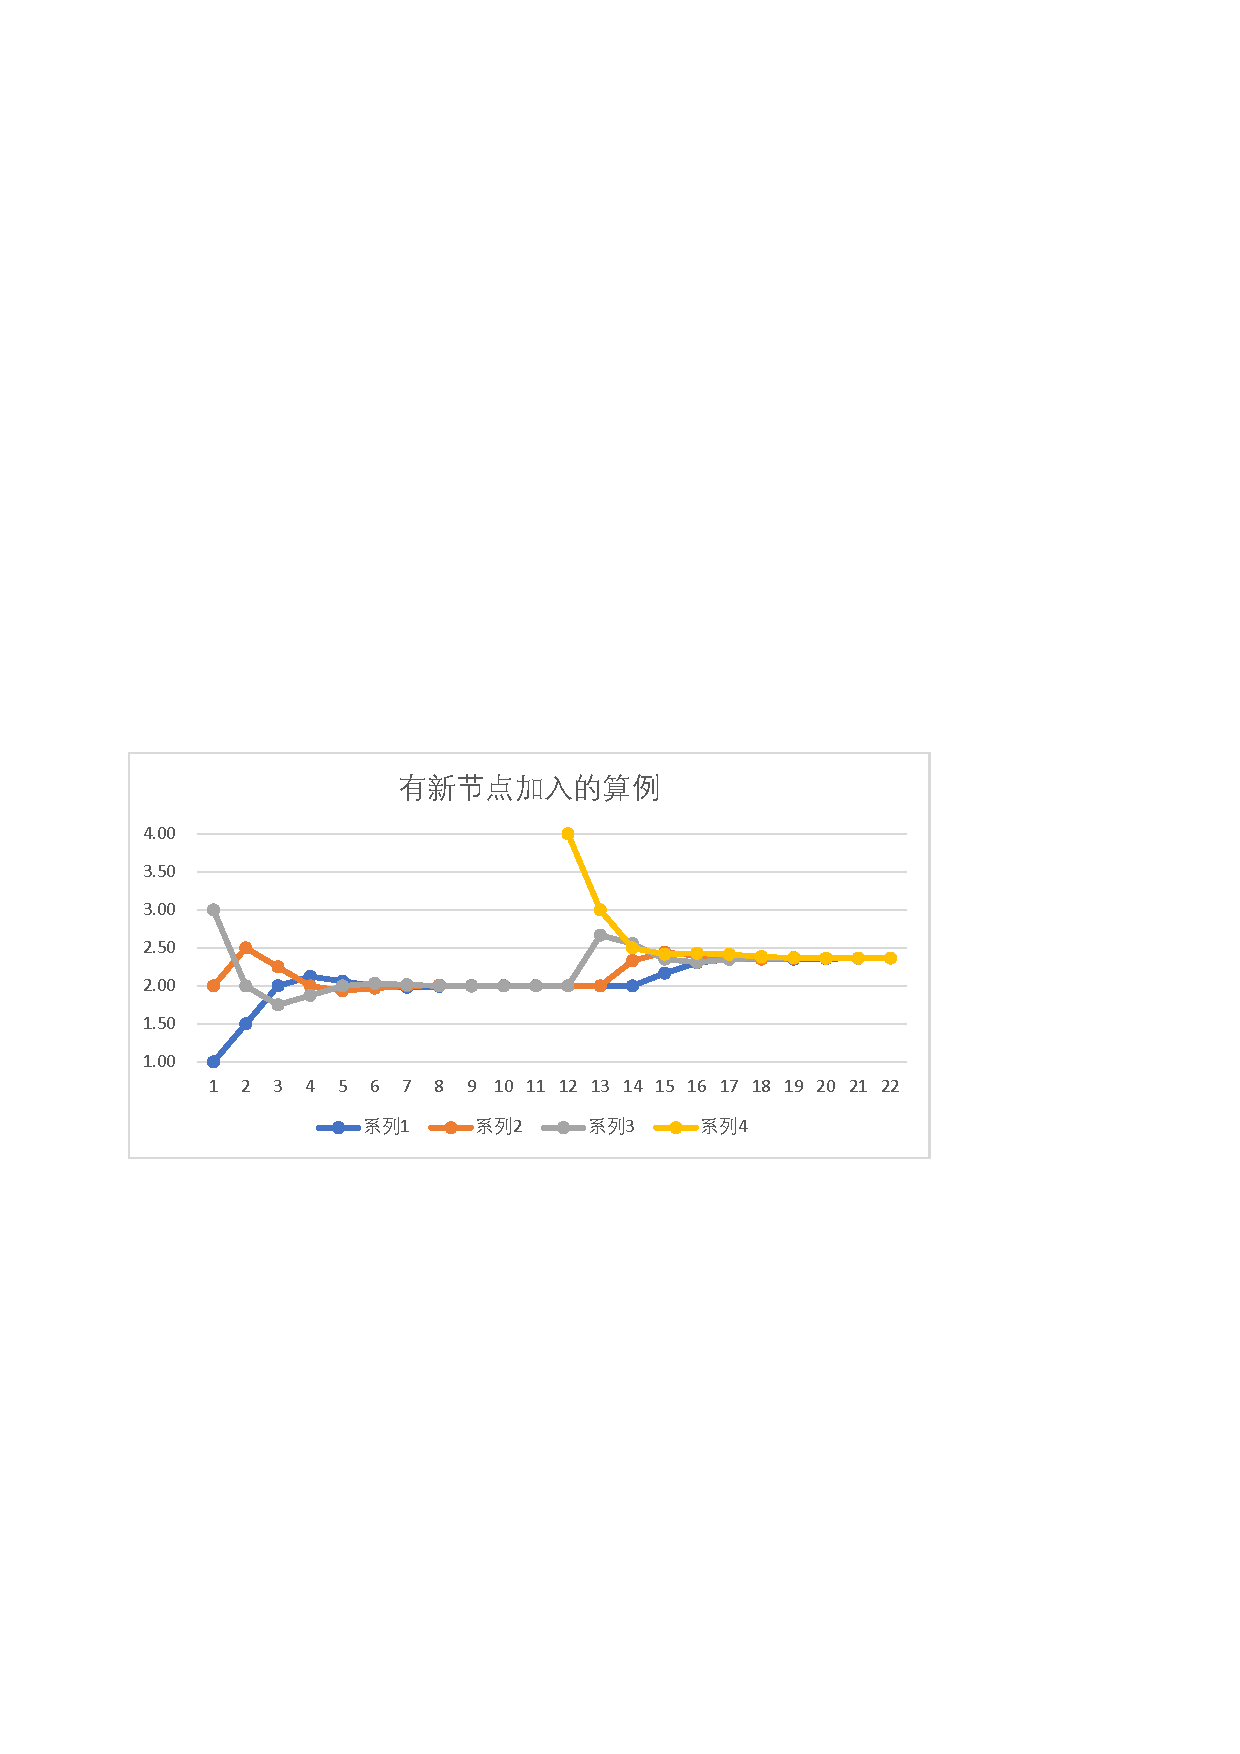
\includegraphics{123-2224.pdf}
    \caption{加入新节点曲线}
    \label{fig:123-2224}
\end{figure}

\section{动画Illustration设计}
\label{sec:Illustration}

动画Illustration采用Cinema 4D R20 设计渲染。

整个Illustration过程如图~\ref{fig:IllustrationDesign}所示。

\begin{figure}[htbp]
    \centering
    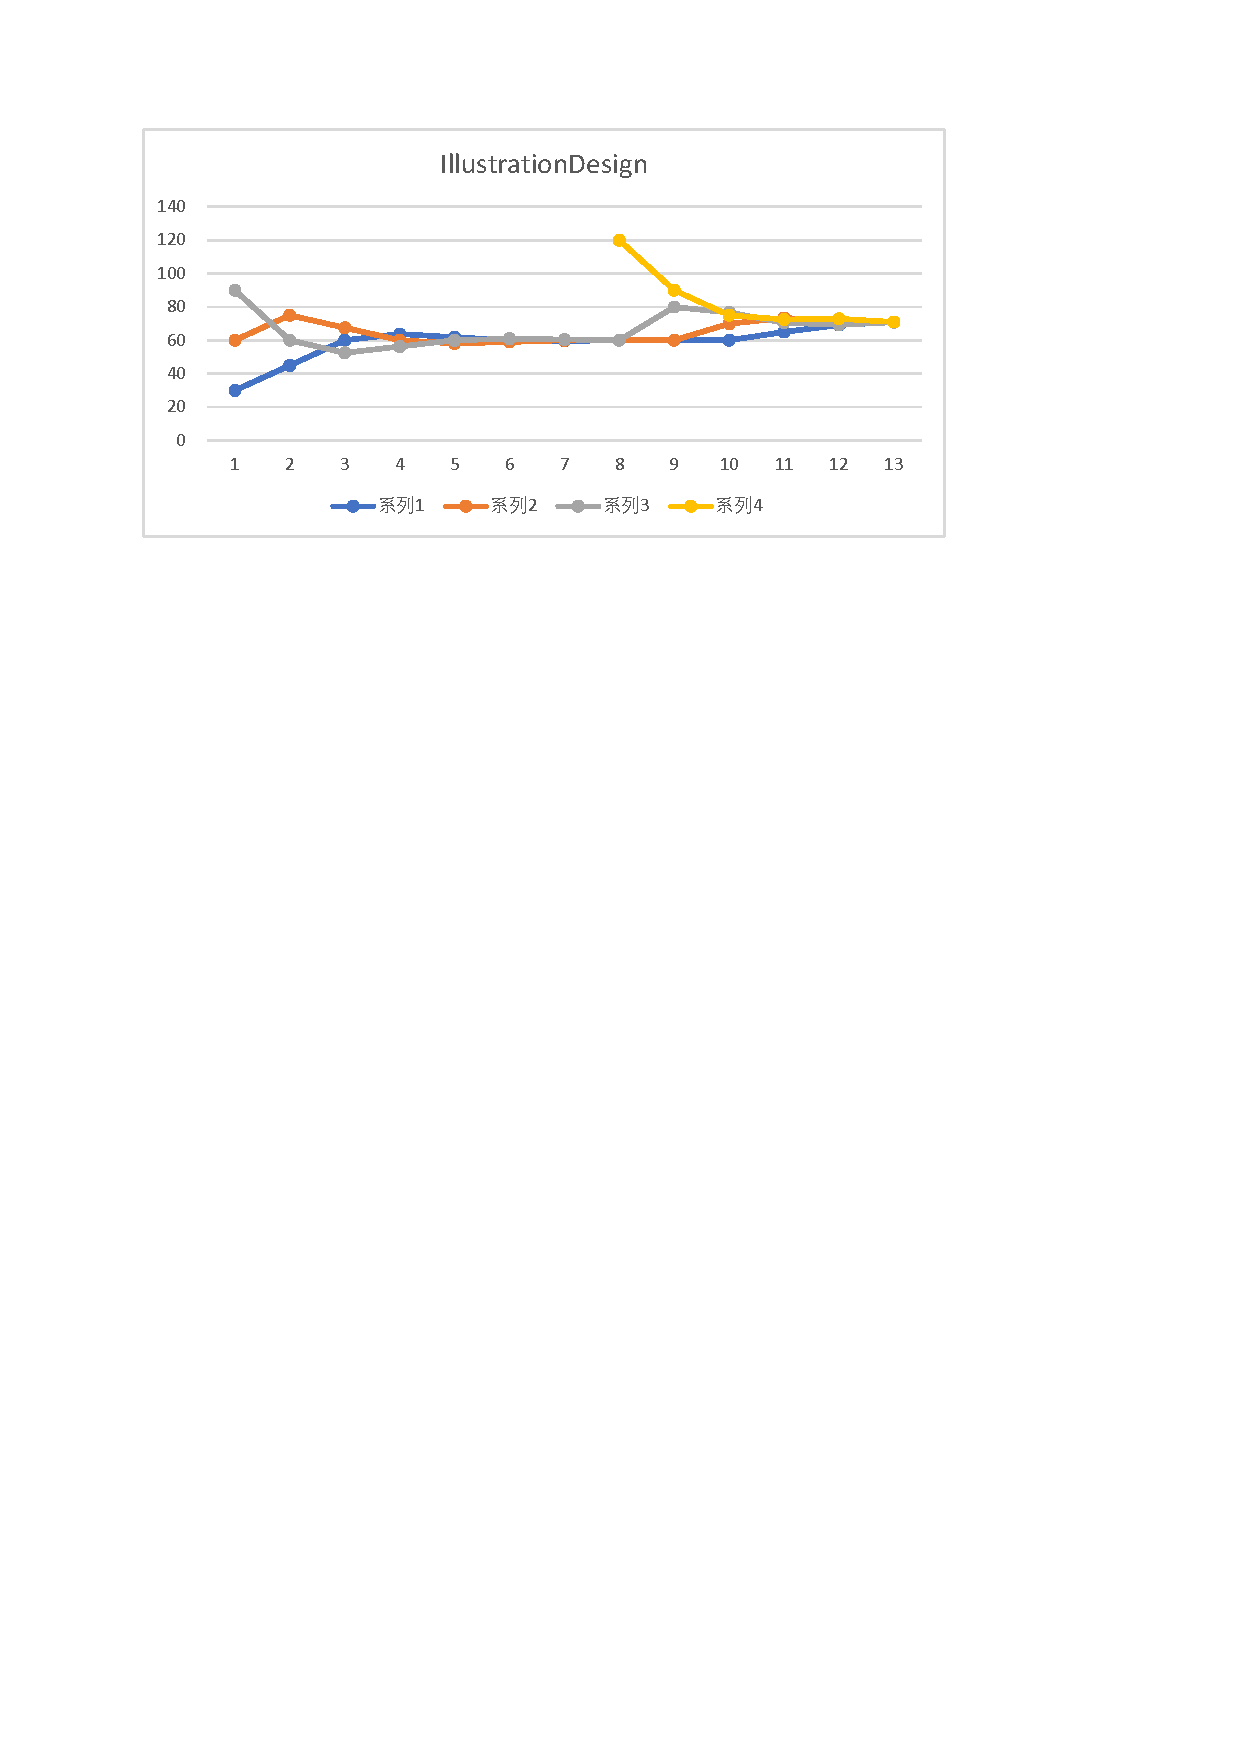
\includegraphics{IllustrationDesign.pdf}
    \caption{IllustrationDesign}
    \label{fig:IllustrationDesign}
\end{figure}

小车外形(包括电池)可以近似视为直径100mm、高80mm的圆柱体,整体画布设置为1m*1m的网格坐标平面;横轴(在C4D中是X轴)相邻间距相等,为20cm;纵轴(在C4D中是Z轴)按照1:30cm缩放比例,即第一个小车初始位置为(1,1)对应到物理坐标系中是(0,30cm)。

时序方面,为了保证视频质量,C4D工程设置里我设置了帧速率(FPS)为60,即60帧/s,虽然这样渲染时间会变长。C4D做动画时间轴是按帧来的,所以下面的剧本将以帧为单位来写,目前想做的是运动1s停顿1s,再进行下一次迭代。放入新小车时用1s从上向下放入,放完一秒之后再开始运动。

各状态开始时间和对应的帧如表~\ref{tab:IllustrationDesign}

\begin{table}[htbp]
    \centering
    \begin{tabular}{|l|l|l|l|l|l|l|}
    \hline
    \diagbox{迭代次数}{$Y_{i,j}$}{节点编号} %添加斜线表头
              & 1     & 2    & 3   & 4     & Arrival Time & Frame \\ \hline
    0         & 30    & 60   & 90  &       & 0            & 0     \\ \hline
    1         & 45    & 75   & 60  &       & 1            & 60    \\ \hline
    2         & 60    & 68   & 53  &       & 3            & 180   \\ \hline
    3         & 64    & 60   & 56  &       & 5            & 300   \\ \hline
    4         & 62    & 58   & 60  &       & 7            & 420   \\ \hline
    5         & 60    & 59   & 61  &       & 9            & 540   \\ \hline
    6         & 60    & 60   & 60  &       & 11           & 660   \\ \hline
    7         & 60    & 60   & 60  & 120   & 13           & 780   \\ \hline
    8         & 60    & 60   & 80  & 90    & 15           & 900   \\ \hline
    9         & 60    & 70   & 77  & 75    & 17           & 1020  \\ \hline
    10        & 65    & 73   & 71  & 73    & 19           & 1140  \\ \hline
    11        & 69    & 72   & 69  & 73    & 21           & 1260  \\ \hline
    12        & 71    & 71   & 71  & 71    & 23           & 1380  \\ \hline
    Color     & White & Blue & Red & Green &              &       \\ \hline
    X-Axis/cm & 0     & 30   & 60  & 90    &              &       \\ \hline
    \end{tabular}
    \caption{各状态开始时间}
    \label{tab:IllustrationDesign}
\end{table}

注意C4D的操作:调视角要按住视图右上角的按钮再拖,调时间轴也是按住小三角拖。直线名为引导线。

设定动画运动路径如图~\ref{fig:C4D-1}所示。

\begin{figure}[htbp]
    \centering
    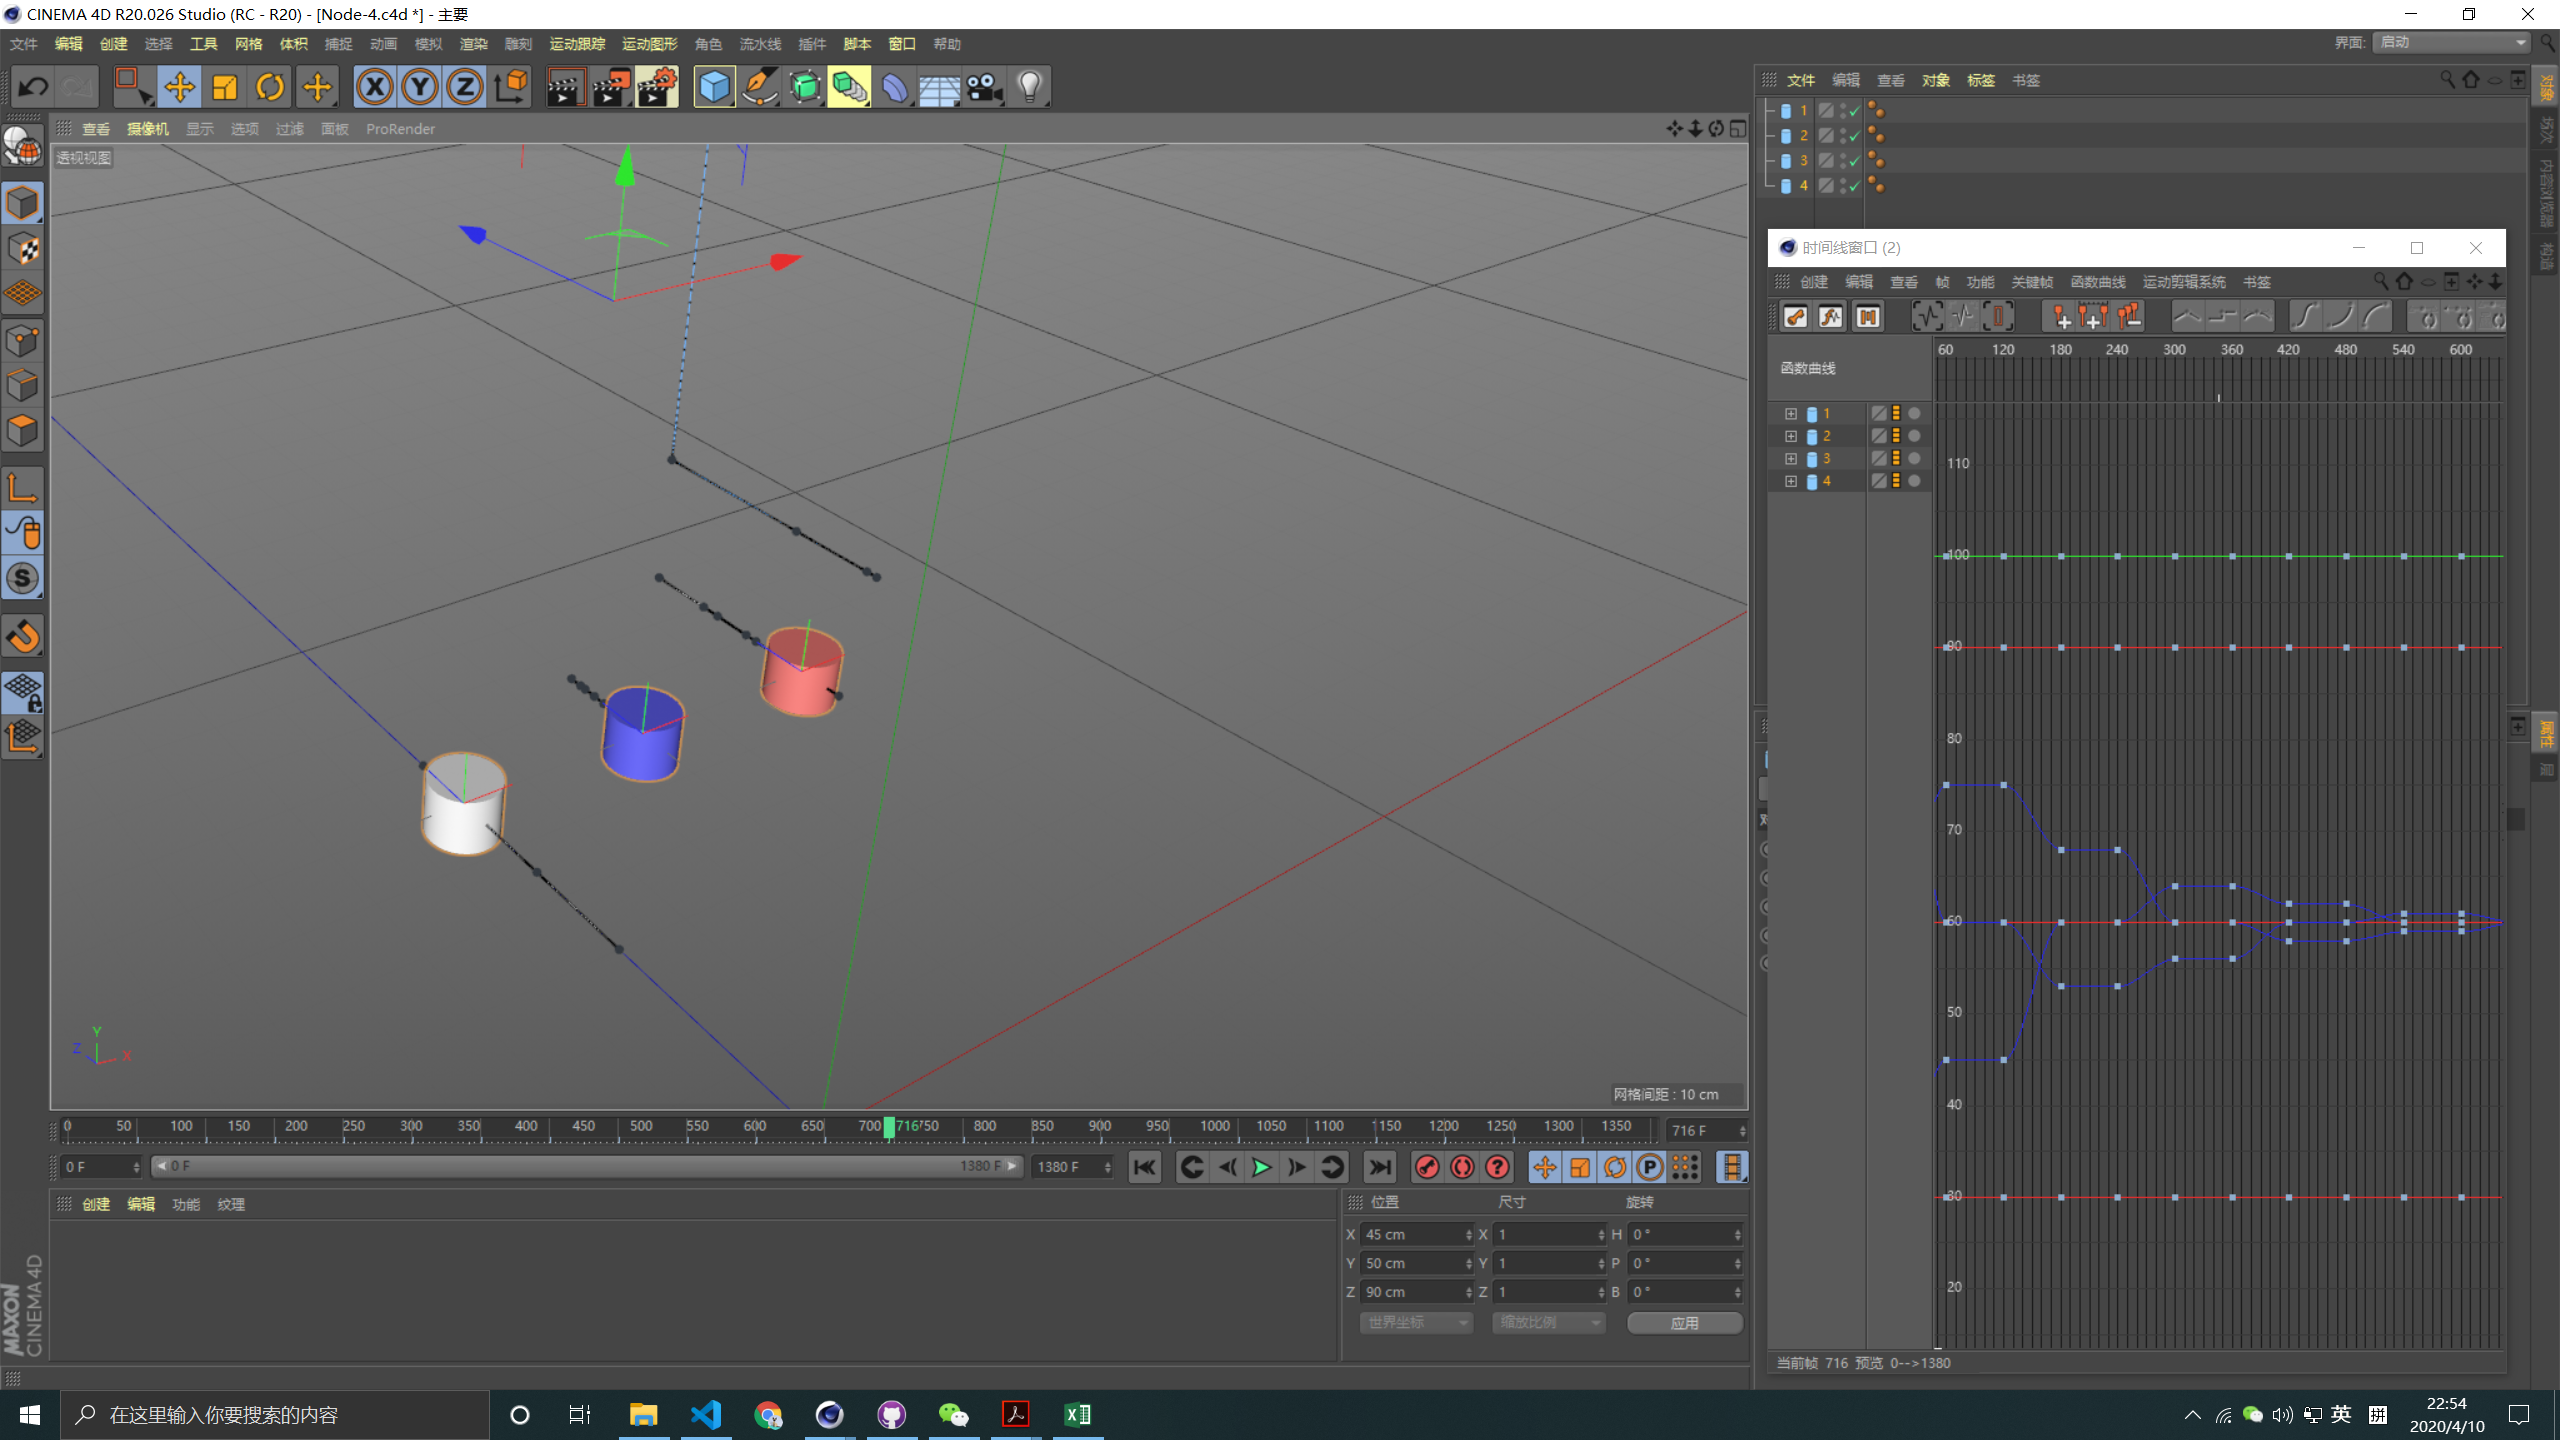
\includegraphics[width=\columnwidth]{C4D-1.png}
    \caption{C4D设定动画运动路径}
    \label{fig:C4D-1}
\end{figure}

设定网格坐标和渲染方法如图~\ref{fig:C4D-2}所示。

\begin{figure}[htbp]
    \centering
    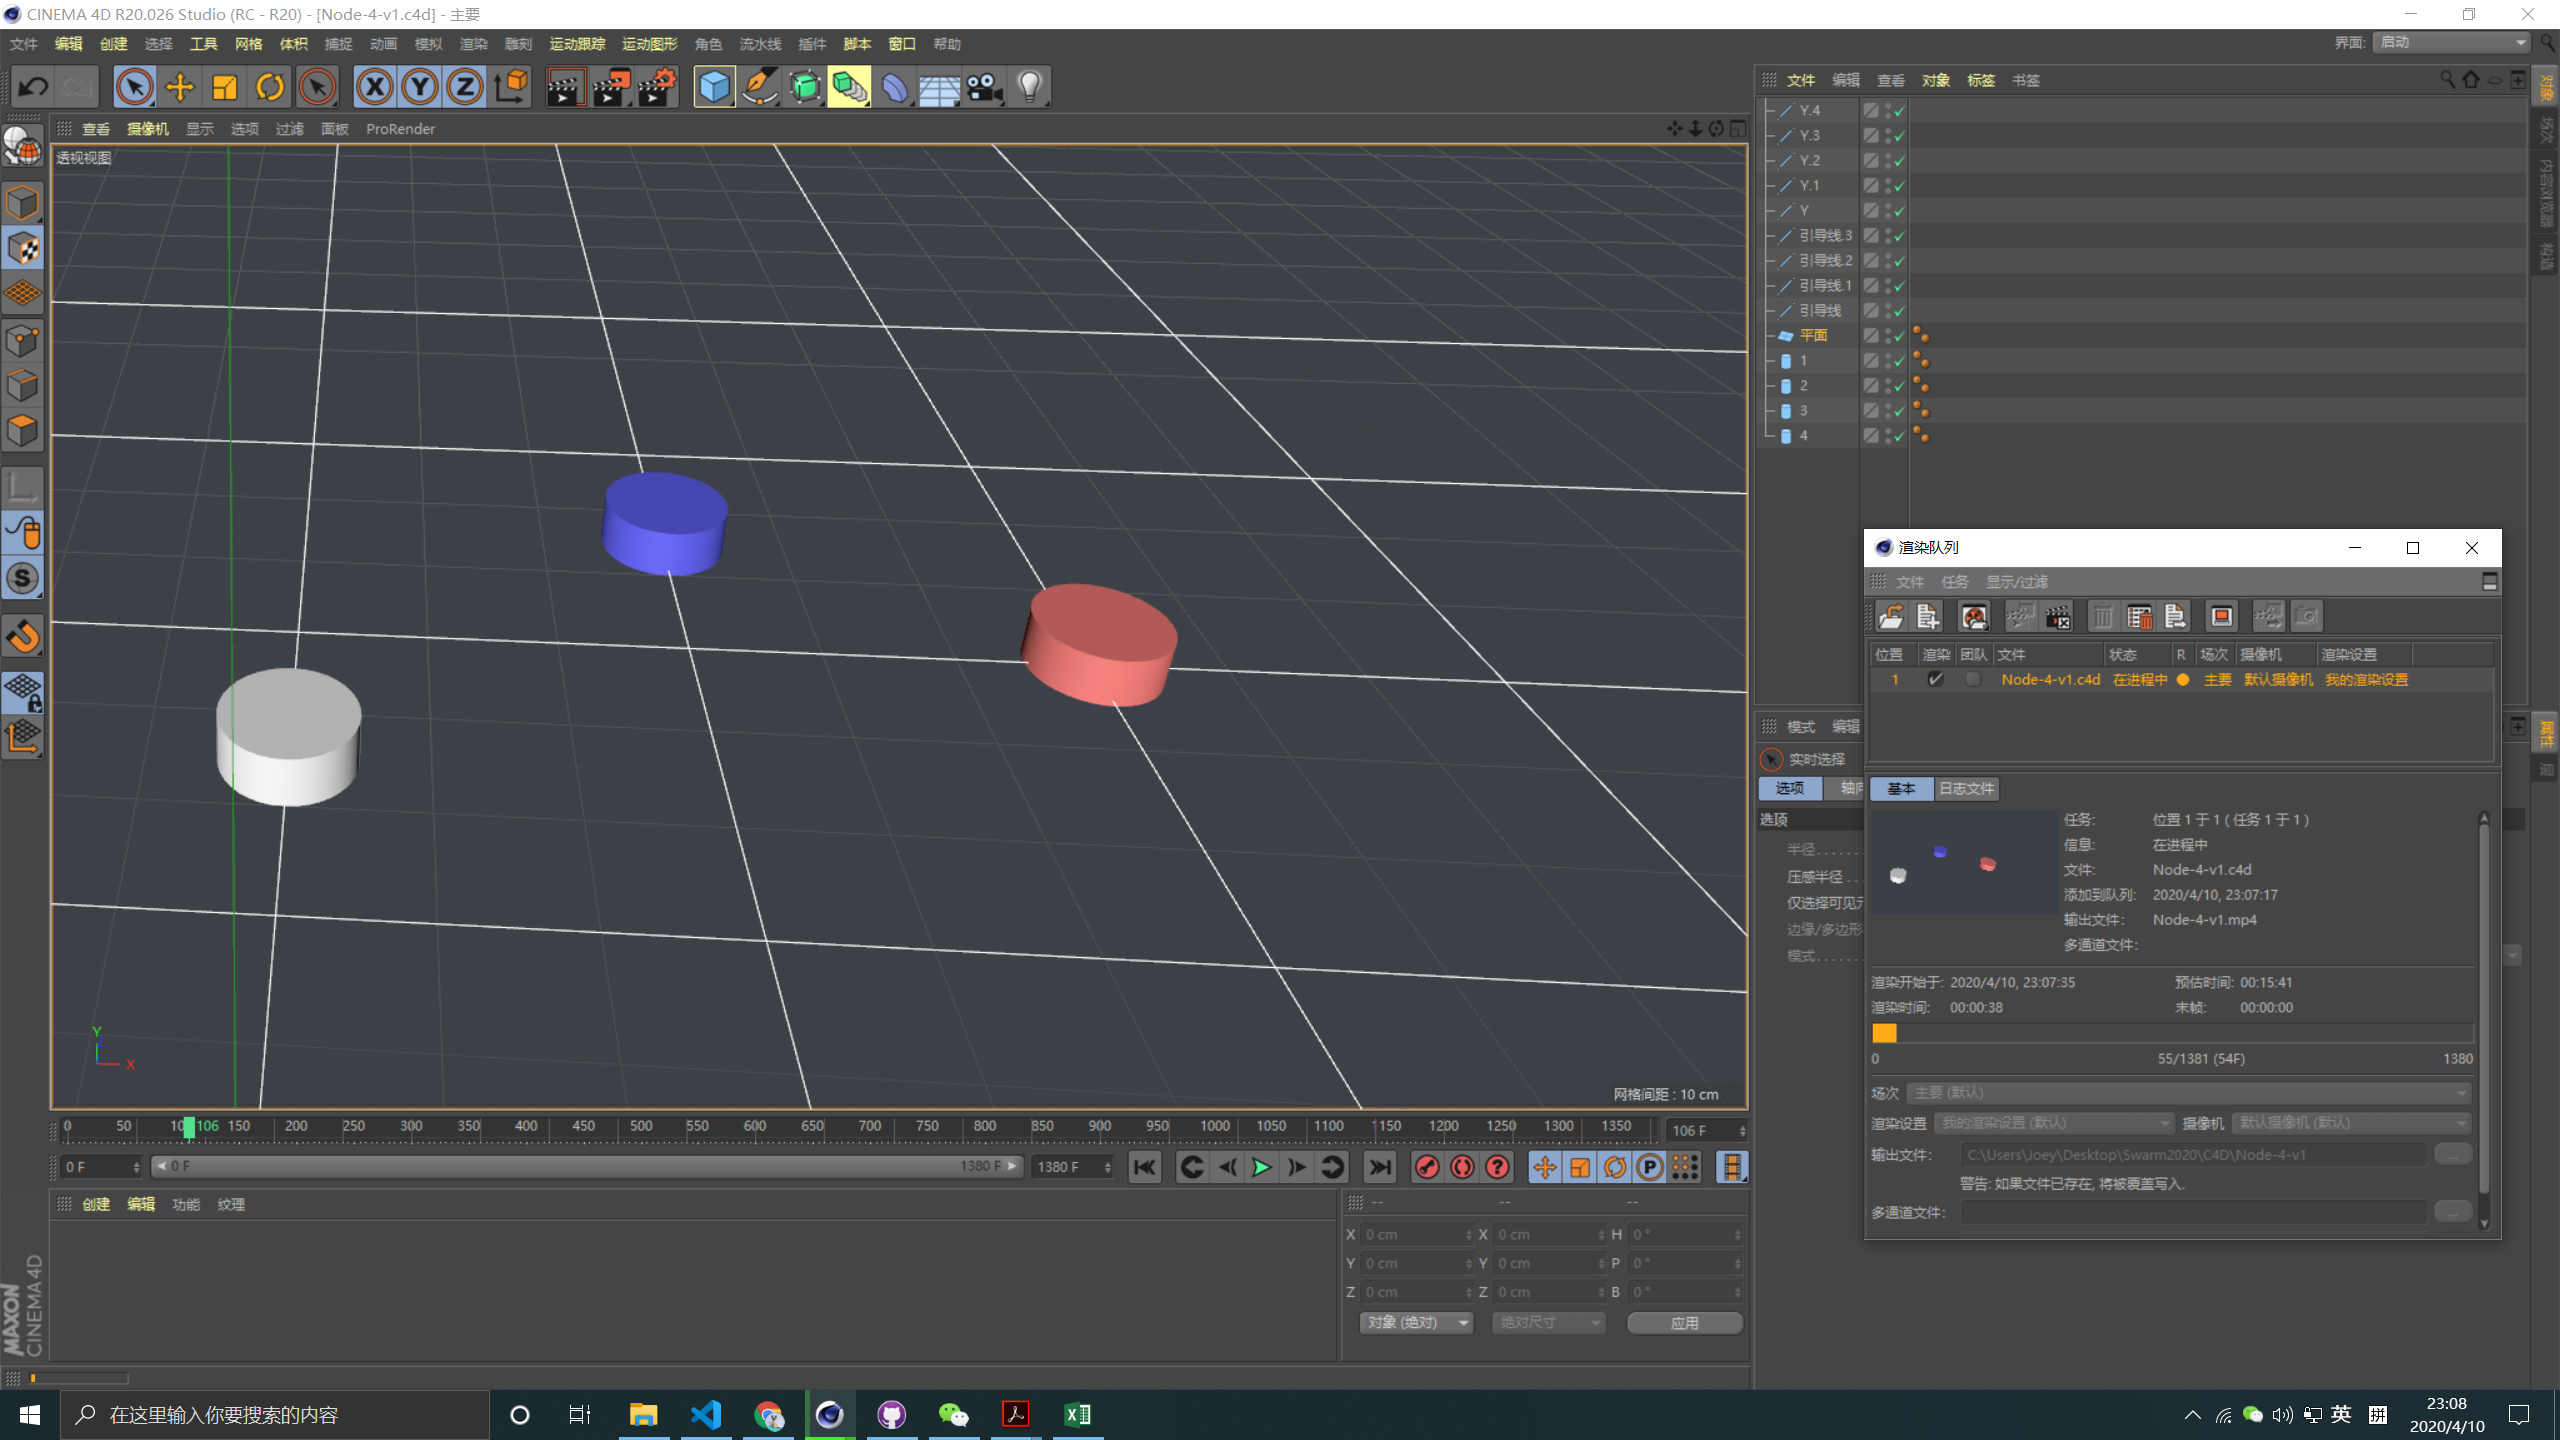
\includegraphics[width=\columnwidth]{C4D-2.png}
    \caption{C4D设定网格坐标和渲染方法}
    \label{fig:C4D-2}
\end{figure}
\chapter{基于马尔可夫链和Perron–Frobenius算法用于分布式电力系统经济调度的过渡矩阵Q优化}
\label{cha:Algorithm}

\section{概述}

本章基于马尔可夫链和Perron–Frobenius算法阐述一种新的用于分布式电力系统经济调度的过渡矩阵Q优化方法,提出了一套完整的分布式ED问题的物理和数学模型,实现了尽可能快的迭代。构建了分布式通信协议,并证明了迭代结束时一定可以得到的是帕累托最优。最后通过一个算例说明了共识达到的具体方法。

\section{分布式经济调度模型}

\subsection{物理模型}

现阶段研究的物理模型公式如式~\ref{eq:phymodel},其中,N是机组数量,$p_{i}$是机组出力,$W_{i}\left(p_{i}\right)$是机组出力成本函数,$\lambda_{i}\left(p_{i}\right)$是边际成本函数,$\alpha_{i}$ $\beta_{i}$ $\gamma_{i}$ 是发电机组出力成本函数中的参数,其中$\alpha_{i}$是机组的假想最低成本,$\beta_{i}$是边际成本关于机组出力边际增长率的倒数,可称是“出力-价格灵敏度”,$\gamma_{i}$是线性外推得到的零边际成本下假想机组出力。$L_{i}$是节点i处的负荷。$\underline{p}_{i}$和$\bar{p}_{i}$分别是机组出力上限与下限。

\begin{equation}
    \begin{aligned}
    &\min W(\mathbf{P})=\sum_{i=1}^{N} W_{i}\left(p_{i}\right)\\
    &\sum_{i=1}^{N} p_{i}=\sum_{i=1}^{N} L_{i}\\
    &\underline{p}_{i} \leq p_{i} \leq \bar{p}_{i}, \forall i\\
    &W_{i}\left(p_{i}\right)=\frac{\left(p_{i}-\alpha_{i}\right)^{2}}{2 \beta_{i}}+\gamma_{i}, i=1,2, \ldots, N\\
    &\lambda_{i}\left(p_{i}\right)=\frac{\partial W_{i}\left(p_{i}\right)}{\partial p_{i}}=\frac{1}{\beta_{i}}\left(p_{i}-\alpha_{i}\right), i=1,2, \ldots, N\\
    &p_{i}=\beta_{i} \lambda_{i}+\alpha_{i}
    \end{aligned}
    \label{eq:phymodel} 
\end{equation}

在边际成本函数的基础上,目标函数等价于求价格共识$\lambda$,其含义是:

\begin{itemize}
    \item 各节点处都有边际成本$\lambda_{i}$,必须保证全部$\lambda_{i}$相等或足够接近。
    \item 在$\lambda_{i}$下,由式~\ref{eq:phymodel}-6决定的机组出力$p_{i}$必须满足全部约束条件。
\end{itemize}

\subsection{数学模型-有向图邻接矩阵}

在图论中,\textbf{图}(Graph)用于表示物件与物件之间的关系,是图论的基本研究对象。一张图由一些小圆点(称为\textbf{顶点}或\textbf{结点})和连结这些圆点的直线或曲线(称为\textbf{边})组成。

如果给图的每条边规定一个方向,那么得到的图称为有向图,其边也称为有向边。在有向图中,与一个节点相关联的边有出边和入边之分,而与一个有向边关联的两个点也有始点和终点之分。相反,边没有方向的图称为无向图。

对有向图而言,顶点的度还可分为出度和入度。一个顶点的出度(Out-degree)为i,是指有i条边以该顶点为起点,或说与该点关联的出边共有i条。入度的概念也类似。

在图论和计算机科学中,邻接矩阵是用于表示有限图的方阵。矩阵的元素指示图中的顶点对是否相邻。

对于顶点集为V的简单图,邻接矩阵为| V | ×| V | 矩阵A使得当存在从顶点i到顶点j的边时元素$A_{ij}$为1,当没有边时为零。矩阵的对角元素全为零,因为在简单图中不允许从顶点到自身的边缘(循环)。在代数图论中有时用代数变量代替非零元素也很有用。

通过将每个两个顶点之间的边数存储在相应的矩阵元素中,并允许非零对角元素,可以将相同的概念扩展到带循环的多重图和图形。只要遵循一致的约定,就可以将循环计数一次(作为单个边)或两次(作为两个顶点边的入射)。无向图通常使用计数循环次数的后一种约定,而有向图通常使用前一种约定。

在有向图中,可以通过对相应列的条目求和来计算顶点的入度,而可以通过对相应行的条目求和来计算顶点的出度。

\begin{figure}
    \begin{minipage}{0.48\textwidth}
      \centering
      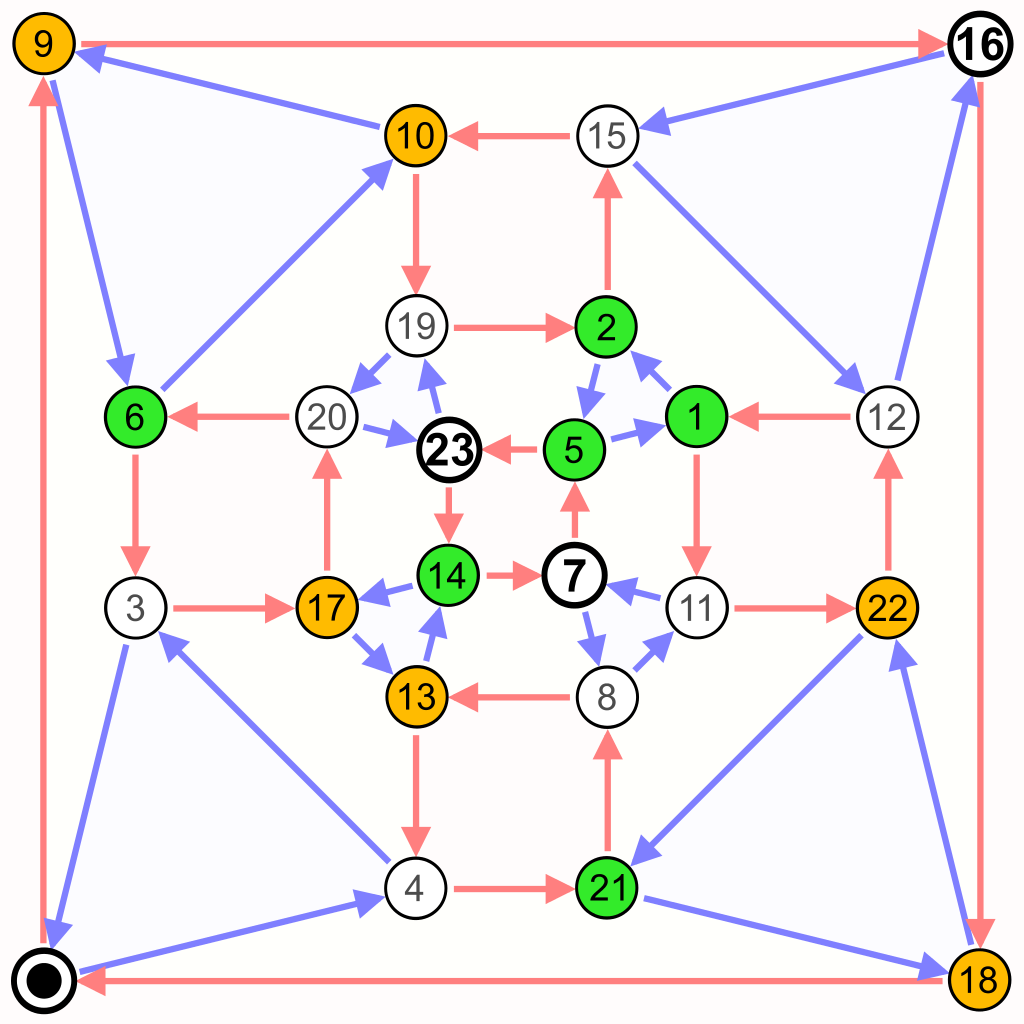
\includegraphics[height=7cm]{numbers.png}
      \caption{Cayley有向图}
      \label{fig:Directed-Cayley-graph}
    \end{minipage}\hfill
    \begin{minipage}{0.48\textwidth}
      \centering
      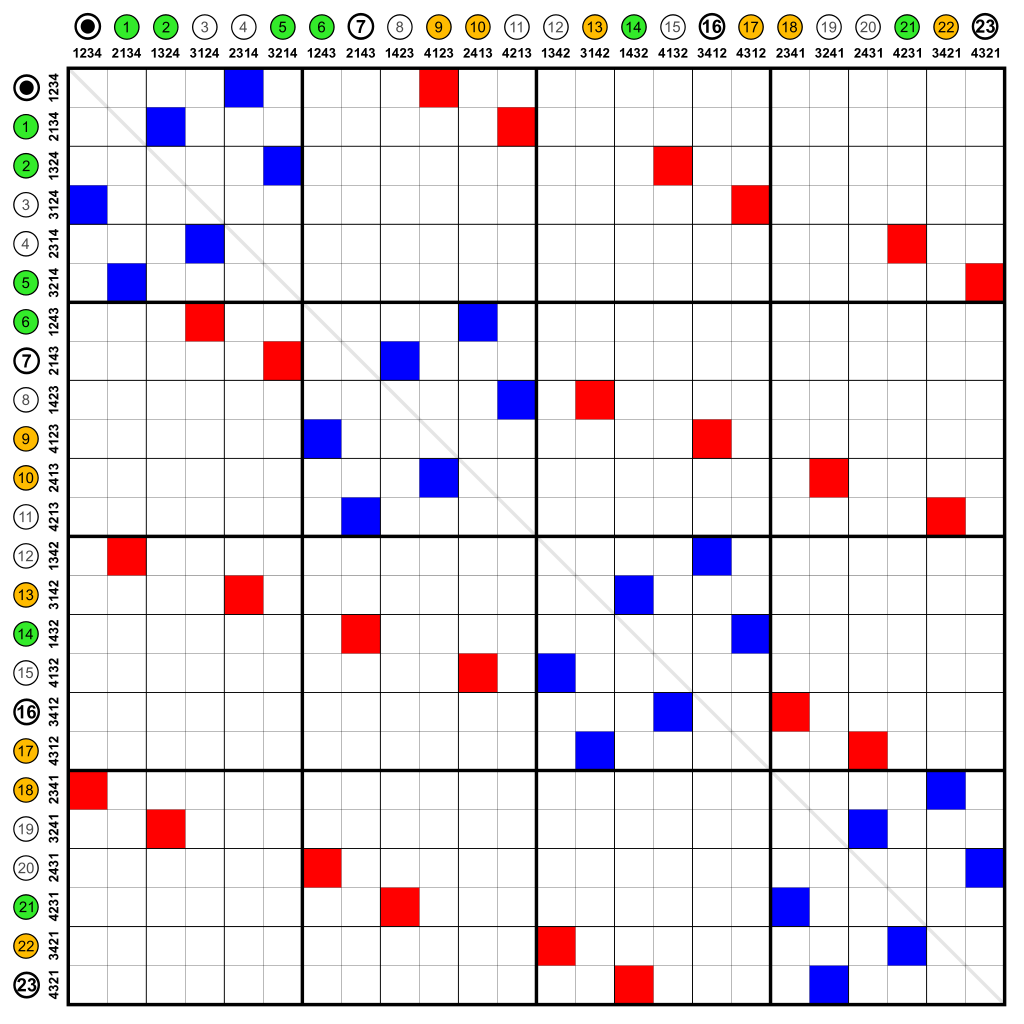
\includegraphics[height=7cm]{adjacency_matrix.png}
      \caption{邻接矩阵}
      \label{fig:Adjacency-matrix}
    \end{minipage}
\end{figure}

\subsection{链式通信协议}
对于一个强连通的电网,我们使用有向图的邻接矩阵A来描述其通信拓扑:

\begin{equation}
    \mathbf{A}=\left[a_{i j}\right]_{N \times N}
\end{equation}

\begin{equation}
    a_{i j}=\left\{\begin{array}{l}
    {1} \\
    {0}
    \end{array}\right.
\end{equation}

其中,1表示通信节点j能向i发送消息并被i接收。

链式通信协议迭代更新每个节点的状态变量如下:

\begin{equation}
    s_{i}^{(k+1)}=\sum_{j=1}^{N} q_{i j} s_{j}^{(k)}, i=1,2, \ldots, N
\end{equation}

矩阵形式为:

\begin{equation}
    \mathbf{s}^{(k+1)}=\mathbf{Q} \mathbf{s}^{(k)}
\end{equation}

由于在电网中,下一轮迭代的状态变量仅和上一轮迭代的状态变量相关,具有无记忆性。参考Markov chain可得,Q为过渡矩阵,有每一次迭代时有向图的边的权重信息。

在实际物理层中,我们选取状态变量为

\begin{equation}
    s_{i}^{(k)}=p_{i}^{(k)}-\alpha_{i}
\end{equation}

其中,$p_{i}^{(k)}$是第k轮迭代的机组i的出力,$\alpha_{i}$为线性外推得到的零边际成本下的假想机组出力。 $s_{i}^{(k)}$是机组i的溢价出力量,这部分出力将抬高机组的边际成本$\lambda_{i}$。

链式通信协议物理含义为:每一回合,每台机组将自身出力按特定比例转移给相邻节点。

\section{过渡矩阵优化}

由Perron–Frobenius定理可知:过渡矩阵的次大特征值$\sigma_{2}$决定链式通信协议收敛速率,主特征向量$\sigma_{1}$(Perron向量)决定链式通信协议的最终收敛结果。因此引入F-范数$\|\mathbf{Q}\|_{F}$优化过渡矩阵,实现机组出力的合理分配,提高收敛速度。

\subsection{F-范数调整过渡矩阵Q的元素值}

使用特定的矩阵范数(matrix norm,模)来简化之后的迭代运算,这里采用弗罗贝尼乌斯范数(Frobenius norm)或称希尔伯特-施密特范数(Hilbert–Schmidt norm),这个范数可用不同的方式定义:

\begin{equation}
    \|A\|_{F}=\sqrt{\sum_{i=1}^{m} \sum_{j=1}^{n}\left|a_{i j}\right|^{2}}=\sqrt{\operatorname{trace}\left(A^{*} A\right)}=\sqrt{\sum_{i=1}^{\min \{m, n\}} \sigma_{i}^{2}}
\end{equation}

这里A*表示A的共轭转置,σi是A的奇异值(特征值),并使用了迹函数。弗罗贝尼乌斯范数与Kn上欧几里得范数非常类似,来自所有矩阵的空间上一个内积。

弗罗贝尼乌斯范数是服从乘法的且在数值线性代数中非常有用。这个范数通常比诱导范数容易计算。

在这里有:

\begin{equation}
    \|\mathbf{Q}\|_{F}=\sqrt{\sum_{i=1}^{N} \sum_{i=1}^{N}\left|q_{i j}\right|^{2}}
\end{equation}

\begin{equation}
    \|\mathbf{Q}\|_{F} \geq \sqrt{\sum_{i=1}^{N}\left|\sigma_{i}\right|^{2}}
\end{equation}

\begin{equation}
    1=\left|\sigma_{1}\right| \geq\left|\sigma_{2}\right| \geq \ldots \geq\left|\sigma_{N}\right|
\end{equation}

优化目标函数:

\begin{equation}
    \min \|\mathbf{Q}\|_{F}^{2}=\sum_{i=1}^{N} \sum_{i=1}^{N}\left|q_{i j}\right|
\end{equation}

优化目标函数物理意义:最小化F范数,相当于最小化次大特征值,优化收敛速率

\subsection{过渡矩阵Q的约束}

过渡矩阵Q满足以下约束条件:

\begin{equation}
    \mathbf{Q}=\left[q_{i j}\right]_{N \times N}
\end{equation}

\begin{equation}
    q_{i j}\left\{\begin{array}{l}
    {\geq 0} \\
    {=0}
    \end{array}\right.
\end{equation}

当节点j不能向节点i发送信息时为0

还需要保证总出力不变:

\begin{equation}
    \mathbf{1}^{T} \mathbf{Q}=\mathbf{1}^{T}
\end{equation}

即:

\begin{equation}
    \sum_{j=1}^{N} q_{i j} \beta_{j}=\beta_{i}, i=1,2, \ldots, N
\end{equation}

为使得链式通信协议收敛于过渡矩阵Q,需保证过渡矩阵的Perron向量恰好等于出力-价格灵敏度向量$\boldsymbol{\beta}=\left[\beta_{1}, \beta_{2}, \ldots, \beta_{N}\right]^{T}$,即保证出力比稳定为$\boldsymbol{\beta}_{1}: \boldsymbol{\beta}_{2} \ldots$。其中$\lambda_{i}=p_{i} / \beta_{i}$,即机组i的成本微增率与出力成正比,$\boldsymbol{\beta}$为出力/价格比例系数。

\begin{equation}
    \mathbf{Q} \boldsymbol{\beta}=\boldsymbol{\beta}
\end{equation}

即:

\begin{equation}
    \sum_{j=1}^{N} q_{i j} \beta_{j}=\beta_{i}, i=1,2, \ldots, N
\end{equation}

\subsection{过渡矩阵优化求解}

即求解以下二次规划问题:

\begin{equation}
    \begin{aligned}
    &\min _{q_{y}}\|\mathbf{Q}\|_{F}^{2}=\sum_{i=1}^{N} \sum_{i=1}^{N}\left|q_{i j}\right|^{2}\\
    &\text { s.t. } \quad q_{i j}\left\{\begin{array}{ll}
    {\geq 0} & {\quad a_{i j}=1} \\
    {=0} & {\quad a_{i j}=0}
    \end{array}\right.\\
    &\mathbf{1}^{T} \mathbf{Q}=\mathbf{1}^{T}\\
    &\mathbf{Q} \boldsymbol{\beta}=\boldsymbol{\beta}
    \end{aligned}
\end{equation}

一般二次规划问题求解形式为:

\begin{equation}
    \begin{aligned}
    &\min \mathbf{x}^{T} \mathbf{x}\\
    &\text { s.t. } \quad \mathbf{A}_{1} \mathbf{x}=\mathbf{b}_{1}
    \end{aligned}
\end{equation}

其中x的每一个元素即是过渡矩阵Q的一个非零元素。该二次规划问题的优化解为:

\begin{equation}
    \mathbf{x}^{*}=\mathbf{A}_{1}^{T}\left(\mathbf{A}_{1} \mathbf{A}_{1}^{T}\right)^{-1} \mathbf{b}_{1}
\end{equation}

将x*的每个元素的值还原到过渡矩阵Q的相应位置上,可得到经优化的过渡阵。

\section{分布式ED协议的实现方式}

每个节点独立算出$\beta_{i}$出力/价格比例系数,

出力-价格灵敏度向量$\boldsymbol{\beta}$与邻接矩阵$\boldsymbol{A}$结合,得出优化后的过渡矩阵$\boldsymbol{Q}$

根据过渡矩阵与链式通信拓扑有向图权重的对应关系,的第j列元素代表始端节点与机组j的边的权重。因此把过渡矩阵$\boldsymbol{Q}$按列拆分,将第j列元素发送给机组j的节点。

节点i独立算出其初始溢价出力量$s_{i}^{(0)}=L_{i}-\alpha_{i}$

按过渡矩阵Q,迭代运行链式通信协议。

\begin{equation}
    s_{i}^{(k+1)}=\sum_{j=1}^{N} q_{i j} s_{j}^{(k)}, i=1,2, \ldots, N
\end{equation}

节点j计算出$q_{i j} s_{j}^{(k)}, i=1,2, \ldots, N$,并分别将$q_{i j} s_{j}^{(k)}$发给节点i。(若$A_{i j}$为0,则此项为0,不影响其他节点)

k次迭代后,节点i的出力和电价为:

\begin{equation}
    \begin{aligned}
    &p_{i}^{(k)}=s_{i}^{(k)}+\alpha_{i}\\
    &\lambda_{i}^{(k)}=s_{i}^{(k)} / \beta_{i}
    \end{aligned}
\end{equation}

当迭代过程中式~\ref{eq:delta}条件满足,则价格达成共识,可以执行目前的定价。

\begin{equation}
    \left|\lambda_{i}^{(k+1)}-\lambda_{i}^{(k)}\right|<\delta
    \label{eq:delta}    
\end{equation}

其中$\delta$为误差容限,表示电价求解精度。

\section{迭代结束将得到帕雷托最优的证明}

本节证明迭代结束时各节点出力达到帕雷托最优(Pareto Optimality),即在误差允许的范围内ED最优解。

\begin{equation}
    \mathbf{1}^{T} \mathbf{s}^{(k+1)}=\mathbf{1}^{T} \mathbf{Q} \mathbf{s}^{(k)}=\mathbf{1}^{T} \mathbf{s}^{(k)}=\mathbf{1}^{T} \mathbf{s}^{(0)}=\sum_{i=1}^{N}\left(L_{i}-\alpha_{i}\right)
\end{equation}

由于终止时各变量趋于稳定,由Perron-由Perron–Frobenius定理:

\begin{equation}
    \mathbf{s}^{(k)}=r \boldsymbol{\beta}
\end{equation}

得:

\begin{equation}
    r=\sum_{i=1}^{N}\left(L_{i}-\alpha_{i}\right) / \sum_{i=1}^{N} \beta_{i}=\lambda_{i}^{(k)}
\end{equation}

表明达到价格共识,并满足功率平衡约束:

\begin{equation}
    \sum_{i=1}^{N}\left(\beta_{i} \lambda_{i}^{(k)}+\alpha_{i}\right)=\sum_{i=1}^{N} L_{i}
\end{equation}

\section{考虑每个节点出力上下限的处理}

当某节点的出力超上下限时,可用虚拟功率法调整出力分配。

\begin{equation}
    S_{i}^{(k+1)}=\left(\sum_{j=1}^{n} q_{i j}\left(s_{j}^{(k)}+\Delta p_{j}^{(k)}\right)\right)-\Delta p_{i}^{(k)}
\end{equation}

\begin{equation}
    \Delta p_{i}^{(k+1)}=\max \left\{\Delta p_{i}^{(k)}+r_{i}^{(k)}\left(s_{i}^{(k)}+\alpha-\bar{p}_{i}\right), 0\right\}
\end{equation}

k能被t整除时为1,反之为0:

\begin{equation}
    r_{i}^{(k)}=\left\{\begin{array}{l}
    {1} \\
    {0}
    \end{array}\right.
\end{equation}


终止条件增加一条:$\Delta p_{i}^{(k)}=0$

$\Delta p_{i}^{(k)}$为机组i引进的虚拟功率,取值为非负数。当机组i的出力到达上限时,由于向外发送了出力,导致整个系统价格抬高。


\section{算例}

设想一个四节点机组网络有向图如图~\ref{fig:Directed-graph}:

%去除Visio白边:http://www.mamicode.com/info-detail-2181323.html

\begin{figure}[htbp] % use float package if you want it here
    \centering
    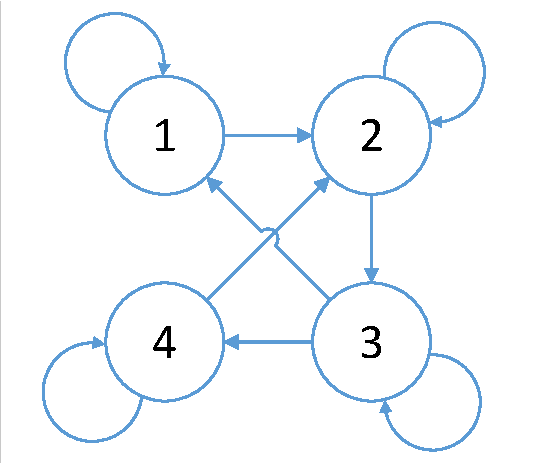
\includegraphics{Directed-graph.pdf}
    \caption{四节点机组网络有向图}
    \label{fig:Directed-graph}
\end{figure}

各节点处机组参数与负荷如表~\ref{tab:example}:

\begin{table}[]
    \centering
%    \resizebox{\textwidth}{!}{%
    \begin{tabular}{@{}ccccc@{}}
    \toprule
    \multicolumn{1}{c}{Node} & $\alpha_{i}(\mathrm{MW})$  & $\beta_{i} \quad\left(\mathrm{MW}^{2} / \mathrm{S}\right)$ & $\gamma_{i}(\mathrm{S})$   & $L_{i}(\mathrm{MW})$    \\ \midrule
    1                        & -1 & 1 & 0.2 & 15.5 \\
    2                        & -2 & 2 & 0.1 & 0    \\
    3                        & -3 & 3 & 0.5 & 15.5 \\
    4                        & -1 & 2 & 0.7 & 0    \\ \bottomrule
    \end{tabular}
%    }缩放表格(字会变得很大)
    \caption{4节点算例机组参数与实时负荷}
    \label{tab:example}
\end{table}

随着迭代各机组的价格曲线如图所示
\chapter{移动平台设计和制造}
\label{cha:Platform}

\section{现有平台对比}

从各类文献和实验平台中总结出各种移动平台的技术参数:


\begin{figure}[htbp]
    \centering
    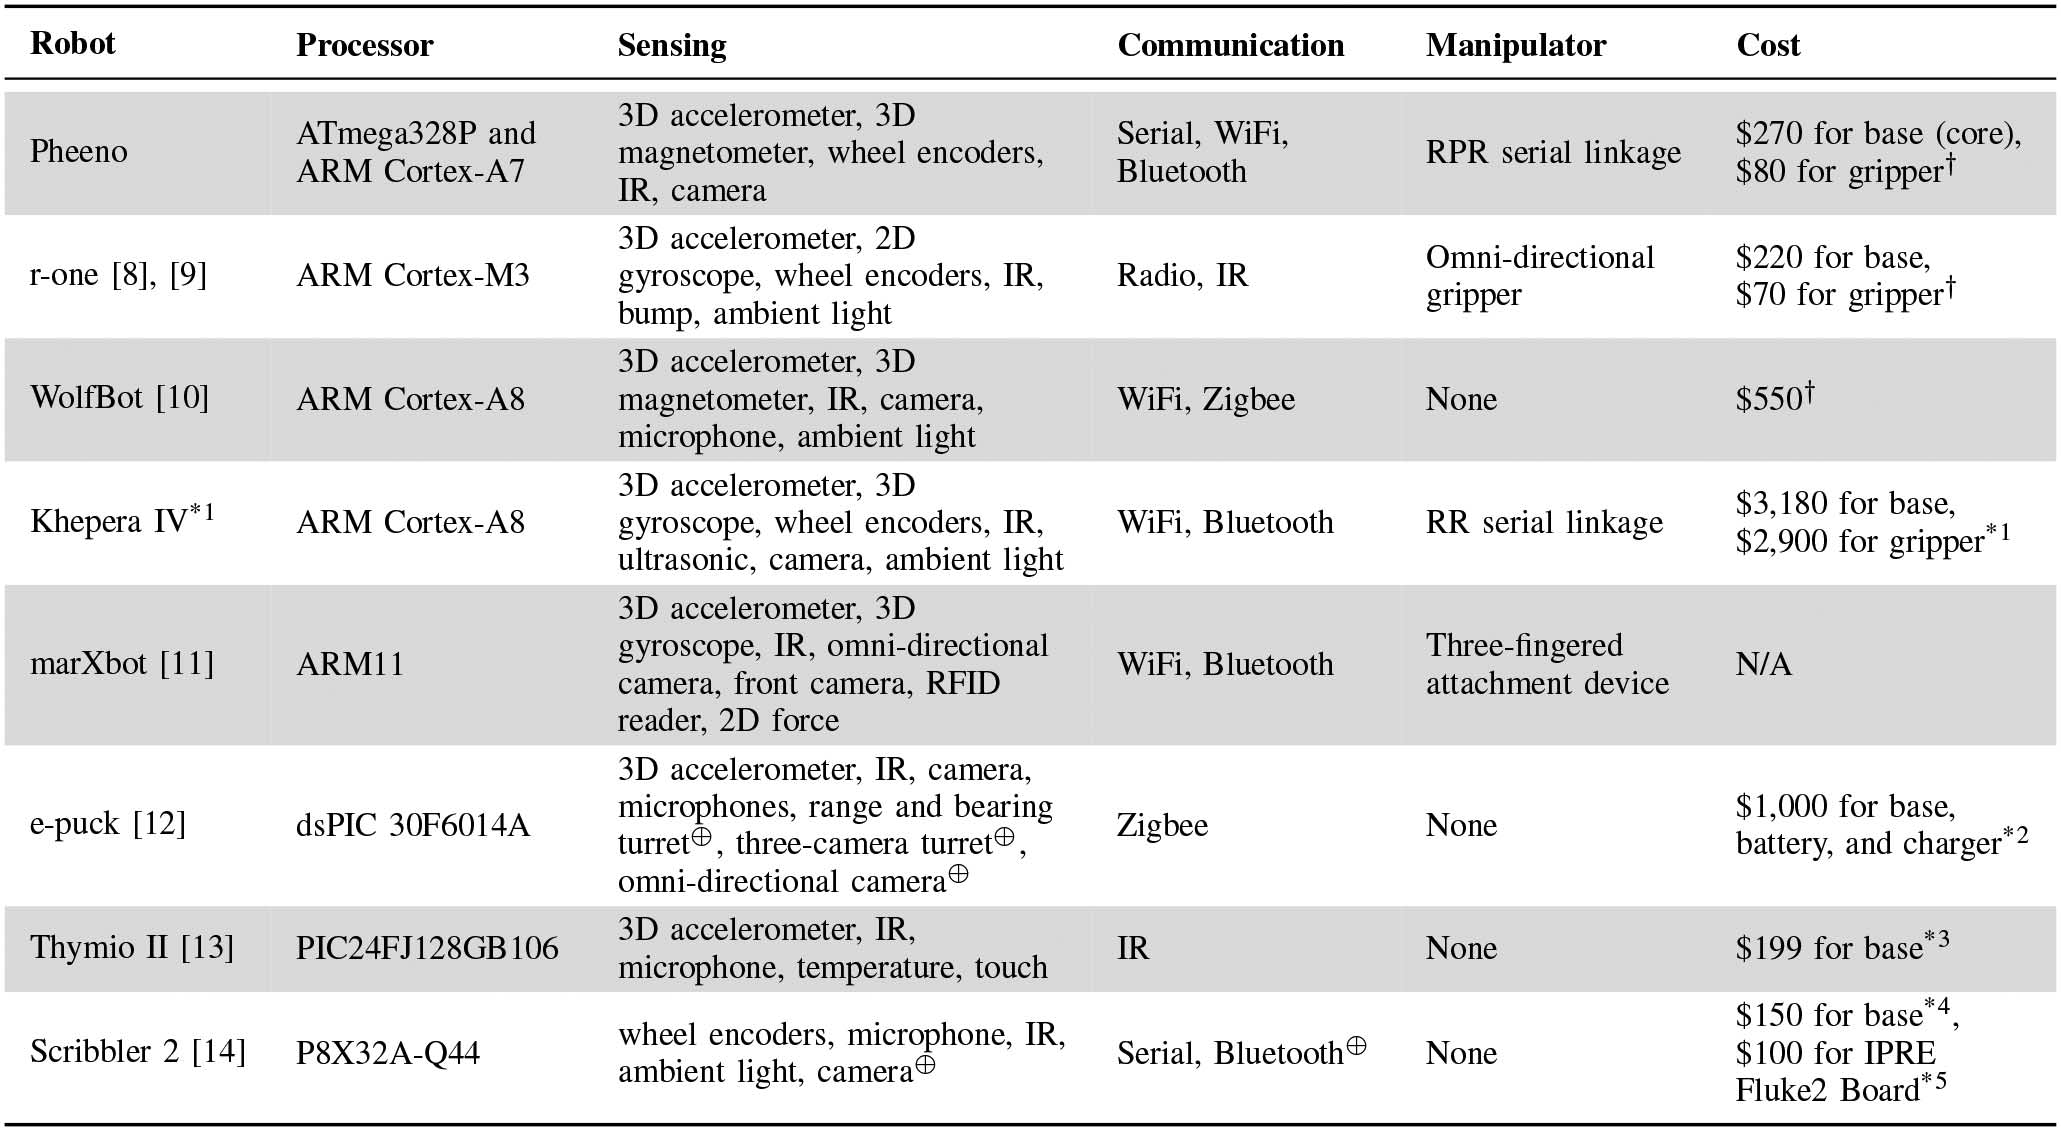
\includegraphics[height=8cm]{Pheeno.jpg}
    \caption{COMPARISON OF CURRENTLY AVAILABLE MULTI-ROBOT PLATFORMS\cite{wilson2016pheeno}}
    \label{fig:Pheeno}
\end{figure}

% Please add the following required packages to your document preamble:
% \usepackage[table,xcdraw]{xcolor}
% If you use beamer only pass "xcolor=table" option, i.e. \documentclass[xcolor=table]{beamer}
% \usepackage{lscape}
\begin{landscape}
    \begin{table}[]
    \centering
    \begin{tabular}{l|lllll}
    \hline
    Name        & Processor                                                                  & Sensing                                                                                                                & Comm.                                                                     & Imaging                                                                              & Cost                 \\ \hline
    \rowcolor[HTML]{EFEFEF} 
    R-One       & \begin{tabular}[c]{@{}l@{}}ARM Cortex-M3, \\ 50 MHz, 64KB RAM\end{tabular} & \begin{tabular}[c]{@{}l@{}}Accelerometer,\\ Gyroscope, Bump, \\ IR, Ambient Light\end{tabular}                         & \begin{tabular}[c]{@{}l@{}}Radio (2 Mbps), \\ IR (1.25 Kbps)\end{tabular} & None                                                                                 & \$220 (Parts)        \\
    E-puck      & \begin{tabular}[c]{@{}l@{}}dsPIC 30F6014A, \\ 64MHz, 8KB RAM\end{tabular}  & \begin{tabular}[c]{@{}l@{}}IR, Accelerometer, \\ Microphone, Camera\end{tabular}                                       & Serial, Bluetooth, IR                                                     & \begin{tabular}[c]{@{}l@{}}40x40 pixels @ 4 FPS. \\ External processing\end{tabular} & \$340 (Parts)        \\
    \rowcolor[HTML]{EFEFEF} 
    MarXBot     & \begin{tabular}[c]{@{}l@{}}ARM11, 533 MHz, \\ 128MB RAM\end{tabular}       & \begin{tabular}[c]{@{}l@{}}Camera,\\ Accelerometer, \\ Gyroscope, RFID, \\ 2D Force, \\ Microphone\end{tabular}        & WiFi, Bluetooth                                                           & \begin{tabular}[c]{@{}l@{}}Up to 2048x1536\\ pixel s @ 12 FPS\end{tabular}           & N/A                  \\
    Khepera III & \begin{tabular}[c]{@{}l@{}}XScale, 600MHz, \\ 128MB RAM\end{tabular}       & \begin{tabular}[c]{@{}l@{}}IR, Ambient Light,\\ Ultrasonic, Camera\end{tabular}                                        & WiFi, Bluetooth                                                           & 640x480 pixels @ 15 FPS                                                              & \textgreater{}\$2000 \\
    \rowcolor[HTML]{EFEFEF} 
    CITRIC      & \begin{tabular}[c]{@{}l@{}}XScale, 624 MHz, \\ 64MB RAM\end{tabular}       & \begin{tabular}[c]{@{}l@{}}Camera, \\ Microphone\end{tabular}                                                          & Zigbee                                                                    & 1280x1024 pixels @ 15FPS                                                             & \$600                \\
    WolfBot     & \begin{tabular}[c]{@{}l@{}}ARM Cortex-A8, 1GHz, \\ 512MB RAM\end{tabular}  & \begin{tabular}[c]{@{}l@{}}IR, Camera, \\ Microphone, \\ Ambient Light, \\ Accelerometer, \\ Magnetometer\end{tabular} & WiFi, Zigbee                                                              & Up to 1280x720 pixels @ 50 FPS                                                       & \$550 (Parts)       
    \end{tabular}
    \caption{Mobile Sensing Platform Comparison\cite{betthauser2014wolfbot}}
    \label{tab:Comparison}
    \end{table}
\end{landscape}



% Please add the following required packages to your document preamble:
% \usepackage{lscape}
\begin{landscape}
    \begin{table}[]
    \centering
    \begin{tabular}{l|lllllll}
    \hline
    robot/author     & size          & battery                                                             & mobility    & perception                                                                  & interaction                                                         & comm.           & processing  \\ \hline
    Jasmine          & 2.6x2.6x2.6cm & \begin{tabular}[c]{@{}l@{}}LiPo, \\ 2 h autonomy\end{tabular}       & wheels      & none                                                                        & none                                                                & radio           & none        \\
    AmigoBot         & 33x28x15cm    & \begin{tabular}[c]{@{}l@{}}Pb, 26Wh,\\ 2 h autonomy\end{tabular}    & wheels      & \begin{tabular}[c]{@{}l@{}}ultrasound, \\ opt. vision\end{tabular}          & none                                                                & opt. radio      & ad hoc      \\
    Kobot            & 12x7cm        & \begin{tabular}[c]{@{}l@{}}LiPo, 7Wh,\\ 10 h autonomy\end{tabular}  & wheels      & opt. omnicam                                                                & none                                                                & Xbee            & opt. PXA255 \\
    Zeero            & $\sim$25 cm   & 4xAA, 9Wh                                                           & wheels      & \begin{tabular}[c]{@{}l@{}}pan-tilt CMUcam2, \\ ultrasound, IR\end{tabular} & none                                                                & Bluetooth       & PXA255      \\
    FlockBots        & 18cm          & \begin{tabular}[c]{@{}l@{}}NiMH, 16Wh, \\ 2 h autonomy\end{tabular} & wheels      & \begin{tabular}[c]{@{}l@{}}pan-tilt CMUCam2, \\ IR\end{tabular}             & simple grip-per                                                     & Wi-Fi           & PXA255      \\
    Molecubes        & 66x66x66cm    & \begin{tabular}[c]{@{}l@{}}16 Wh \\ 1 h autonomy\end{tabular}       & opt. wheels & opt. vision                                                                 & \begin{tabular}[c]{@{}l@{}}assembling, \\ gripper\end{tabular}      & opt. Blue-tooth & opt. ARM 11 \\
    Mindart          & 29x24x37cm    & NiCad, 20 Wh                                                        & tracks      & beacon \& vision                                                            & gripper                                                             & none            & Scenix SX   \\
    Yoo, K.H. et al. & n.a.          & n.a.                                                                & tracks      & vision                                                                      & self-assembling                                                     & RF              & off-board   \\
    JL-1             & 35x25x15cm    & 4 h autonomy                                                        & tracks      & vision                                                                      & self-assembling                                                     & Wi-Fi           & PXA255      \\
    S-bot            & 12x15cm       & \begin{tabular}[c]{@{}l@{}}Lion, 10Wh, \\ 2 h autonomy\end{tabular} & treels      & omnicam                                                                     & \begin{tabular}[c]{@{}l@{}}gripper, \\ self-assembling\end{tabular} & Wi-Fi           & PXA255     
    \end{tabular}
    \caption{A selection of robots that have been used recently for collective experiments. The perception column lists the long range (\textgreater 20 cm) sensing capabilities of the robot, which excludes proximity sensors and bumpers. The processing column lists the vision-capable processing unit of the robot (\textgreater 100 MIPS), which excludes microcontrollers.\cite{bonani2010marxbot}}
    \label{tab:collective}
    \end{table}
\end{landscape}



\section{平台设计初始思路}
形式:

每个小车为一个数据点,在1-3维坐标系内动态运动(如果和ShapeBots\cite{suzuki2019shapebots}一样具备升降平台或者和SwarmOS一样具备可变色LED点阵则可以进行三维变量显示)

也可以每个小车作为一个通信节点(在电力市场的应用场景下是一个机组节点),用屏幕/位置/RGB颜色/高度直观的显示迭代的过程。

即插即用的实现:放入/取出小车,新的迭代随即开始。

\section{仿真}

Swarm仿真参考ShapeBots\cite{suzuki2019shapebots}的仿真方法\footnote{\href{https://ryosuzuki.github.io/shapebots-simulator/}{https://ryosuzuki.github.io/shapebots-simulator/}},使用Javascript在网页端编写了相应的仿真程序,进行指定数量的集群小车对于SVG格式图片的渲染和给定数据折线图或条形图的可视化绘制。

\section{定位方法}

% 如果直接插入一页PDF用
% 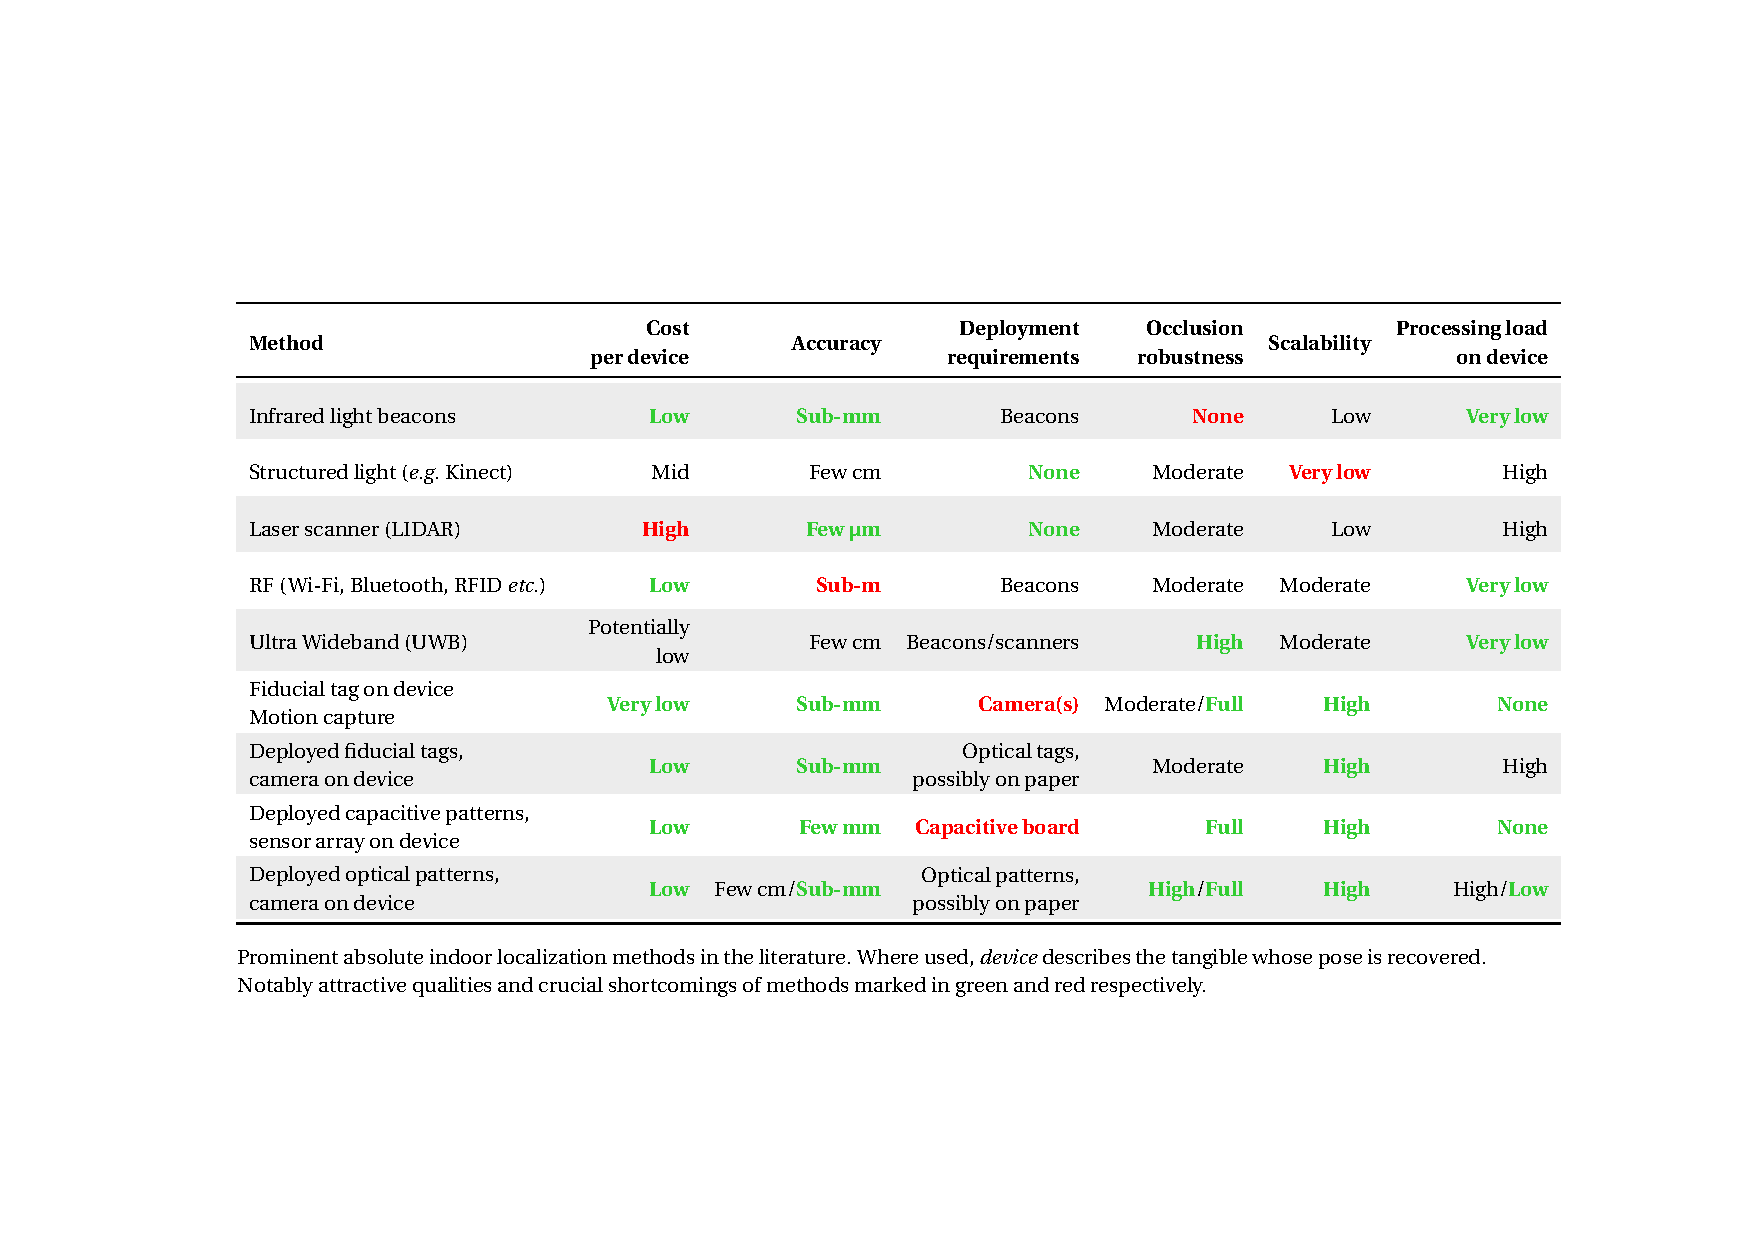
\includepdf{Prominent-absolute-indoor-localization-methods-comparison.pdf} 

% Please add the following required packages to your document preamble:
% \usepackage[table,xcdraw]{xcolor}
% If you use beamer only pass "xcolor=table" option, i.e. \documentclass[xcolor=table]{beamer}
% \usepackage{lscape}
\begin{landscape}
    \begin{table}[]
    \centering
    \begin{tabular}{lllllll}
    \hline
    Method                                                                                         & Cost per device & Accuracy      & \begin{tabular}[c]{@{}l@{}}Deployment\\ requirements\end{tabular}             & \begin{tabular}[c]{@{}l@{}}Occlusion\\ robustness\end{tabular} & Scalabiity & \begin{tabular}[c]{@{}l@{}}Processing load\\ on device\end{tabular} \\ \hline
    \rowcolor[HTML]{EFEFEF} 
    Infrared light beacons                                                                         & Low             & Sub-mm        & Beacons                                                                       & None                                                           & Low        & Very low                                                            \\
    Structured light (e.g. Kinect)                                                                 & Mid             & Few cm        & None                                                                          & Moderate                                                       & Very low   & High                                                                \\
    \rowcolor[HTML]{EFEFEF} 
    Laser scanner (LIDAR)                                                                          & High            & Few µm        & None                                                                          & Moderate                                                       & Low        & High                                                                \\
    \begin{tabular}[c]{@{}l@{}}RF (Wi-Fi, \\ Bluetooth, RFID etc.)\end{tabular}                    & Low             & Sub-m         & Beacons                                                                       & Moderate                                                       & Moderate   & Very low                                                            \\
    \rowcolor[HTML]{EFEFEF} 
    \begin{tabular}[c]{@{}l@{}}Ultra Wideband \\ (UWB)\end{tabular}                                & Potentially low & Few cm        & Beacons/scanners                                                              & High                                                           & Moderate   & Very low                                                            \\
    \begin{tabular}[c]{@{}l@{}}Fiducial tag on device\\ Motion capture\end{tabular}                & Very low        & Sub-mm        & Camera(s)                                                                     & Moderate/Full                                                  & High       & None                                                                \\
    \rowcolor[HTML]{EFEFEF} 
    \begin{tabular}[c]{@{}l@{}}Deployed fiducial tags,\\ camera on device\end{tabular}             & Low             & Sub-mm        & \begin{tabular}[c]{@{}l@{}}Optical tags, \\ possibly on paper\end{tabular}    & Moderate                                                       & High       & High                                                                \\
    \begin{tabular}[c]{@{}l@{}}Deployed capacitive patterns,\\ sensor array on device\end{tabular} & Low             & Few mm        & Capacitive board                                                              & Full                                                           & High       & None                                                                \\
    \rowcolor[HTML]{EFEFEF} 
    \begin{tabular}[c]{@{}l@{}}Deployed optical patterns,\\ camera on device\end{tabular}          & Low             & Few cm/Sub-mm & \begin{tabular}[c]{@{}l@{}}Optical patterns,\\ possibly on paper\end{tabular} & High/Full                                                      & High       & High/Low                                                            \\ \hline
    \end{tabular}
    \caption{Prominent absolute indoor localization methods in the literature. Where used, device describes the tangible whose pose is recovered. }
    \label{tab:localization}
    \end{table}
\end{landscape}

各类定位方法优缺点\cite{ozgur2018cellulo}如表~\ref{tab:localization}所示。

\section{底盘}
考虑到交互过程中需要推动小车,通过用户调查我们知道:大多数用户(特别是儿童)习惯于按压着移动小车,这就使得我们不能采用Zooids\cite{le2016zooids}(如图~\ref{fig:Zooids})或e-puck\cite{mondada2009puck}(如图~\ref{fig:e-puck})使用的差速转向,只能采用类似Cellulo\cite{ozgur2017cellulo}(如图~\ref{fig:Cellulo})的磁驱技术或WolfBot\cite{betthauser2014wolfbot}(如图~\ref{fig:WolfBot})使用的全向轮。

\begin{figure}[htbp]
    \centering
    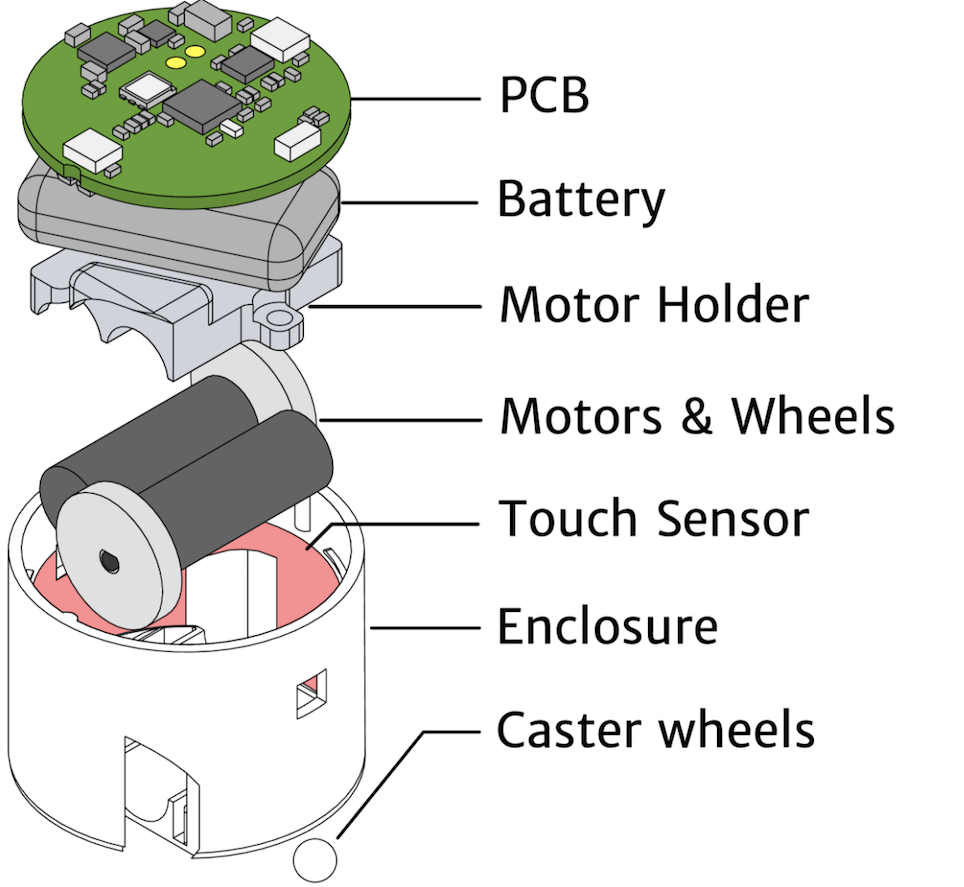
\includegraphics[height=10cm]{Zooids.png}
    \caption{Zooids}
    \label{fig:Zooids}
\end{figure}

\begin{figure}[htbp]
    \centering
    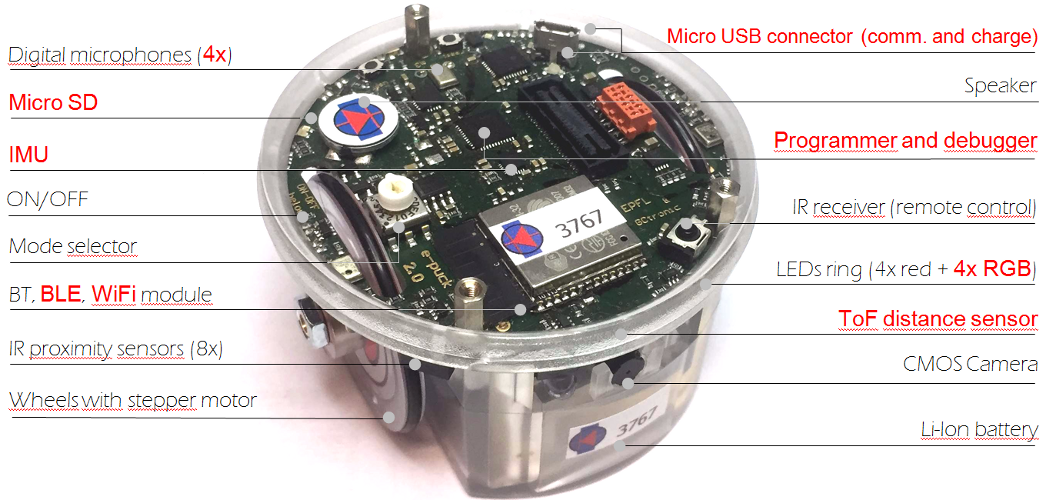
\includegraphics[height=6cm]{e-puck2-features_small.png}
    \caption{Zooids}
    \label{fig:e-puck}
\end{figure}

\begin{figure}[htbp]
    \centering
    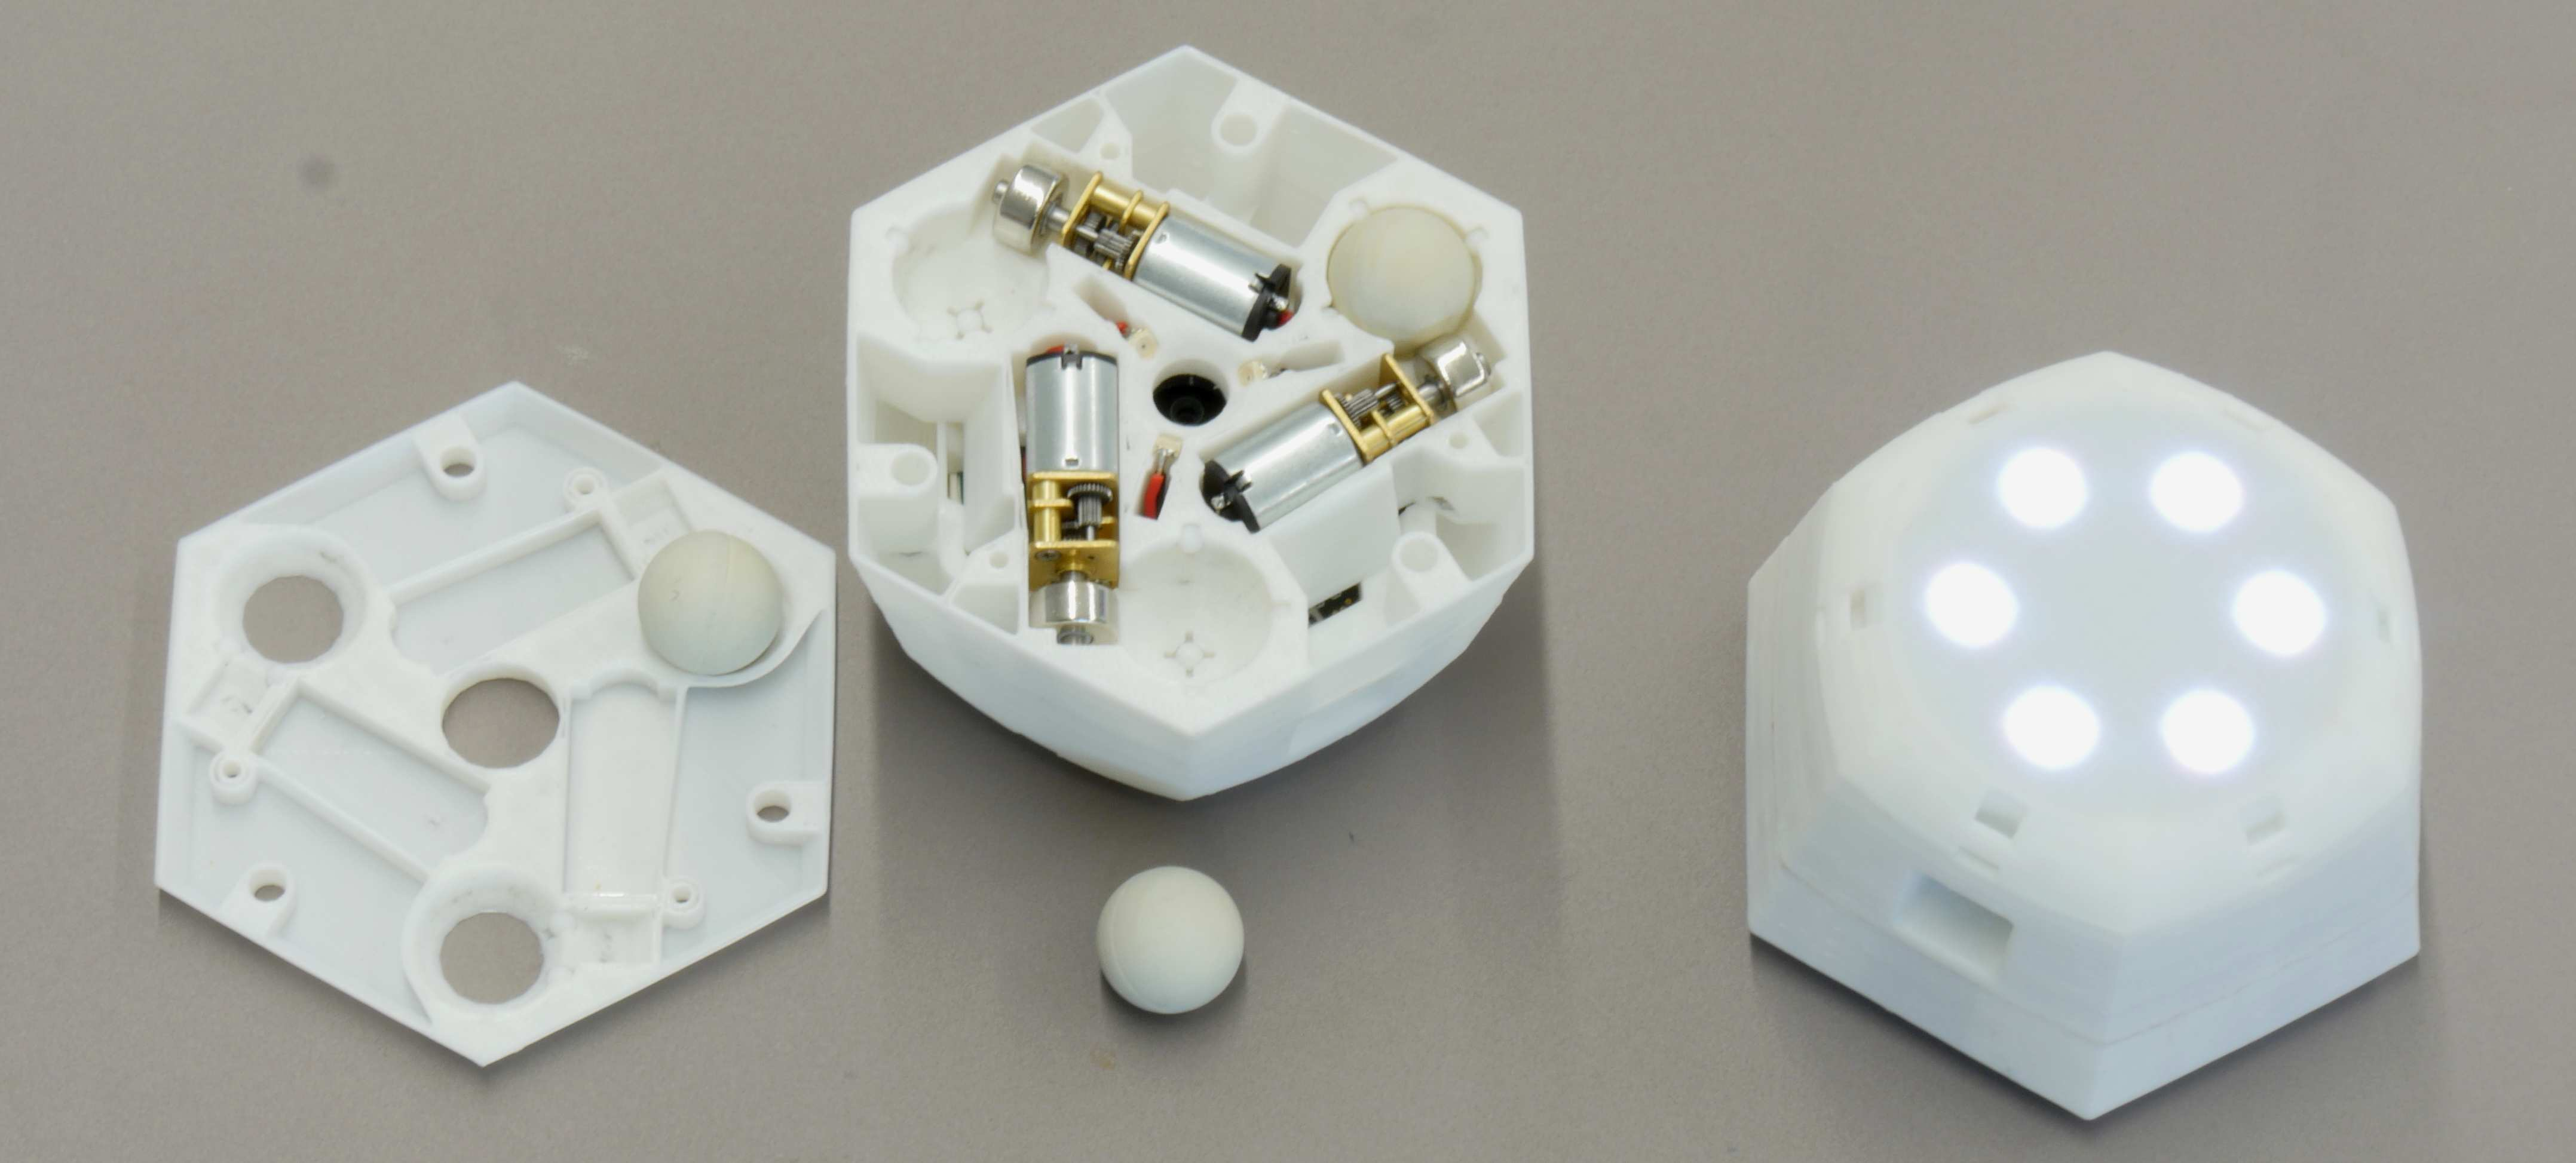
\includegraphics[height=6cm]{cellulo.jpg}
    \caption{Cellulo}
    \label{fig:Cellulo}
\end{figure}
  
\begin{figure}[htbp]
    \centering
    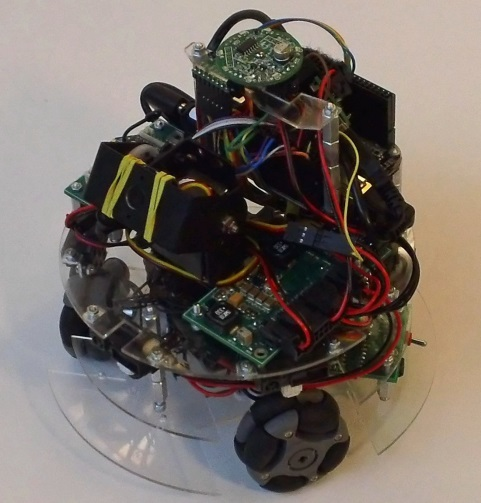
\includegraphics[height=10cm]{WolfBot.jpg}
    \caption{WolfBot}
    \label{fig:WolfBot}
\end{figure}

经过尝试,我们发现磁驱电机的速度和磁环的磁性强弱、电池的电量剩余、磁环和轴之间的胶合强度等不可控因素关系很大,无法建立起小车各轮速度和电机PWM占空比之间的时不变映射关系,导致很难控制小车的走向和速度,最终放弃了这一想法。

WolfBot采用的全向轮和电机直接连接,使得底盘占地面积很大。最终我们则采用1.5英寸麦克纳姆轮(如图~\ref{fig:Wheel})和GW12-N20减速电机(如图~\ref{fig:GM12})(减速齿轮中的蜗杆改变90度传动方向)实现系统最小化。

\begin{figure}
    \begin{minipage}{0.48\textwidth}
      \centering
      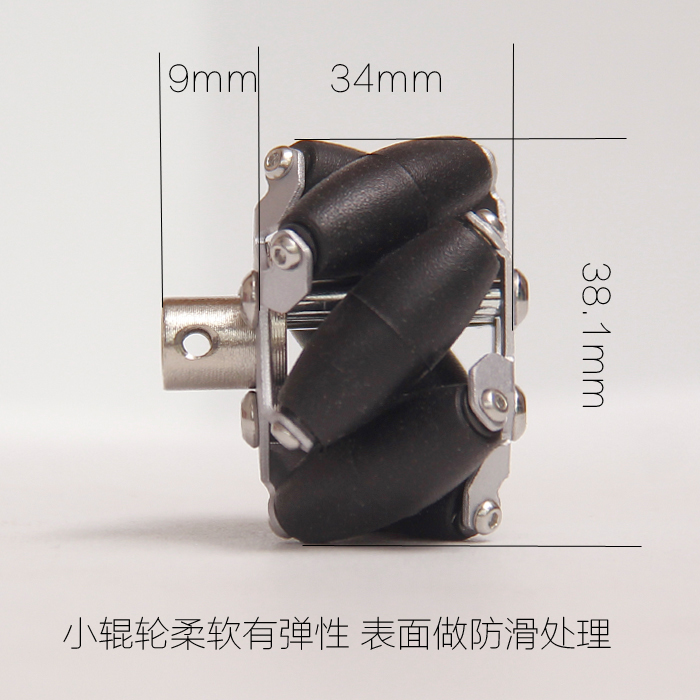
\includegraphics[height=5cm]{Wheel.jpg}
      \caption{使用的1.5英寸麦克纳姆轮}
      \label{fig:Wheel}
    \end{minipage}\hfill
    \begin{minipage}{0.48\textwidth}
      \centering
      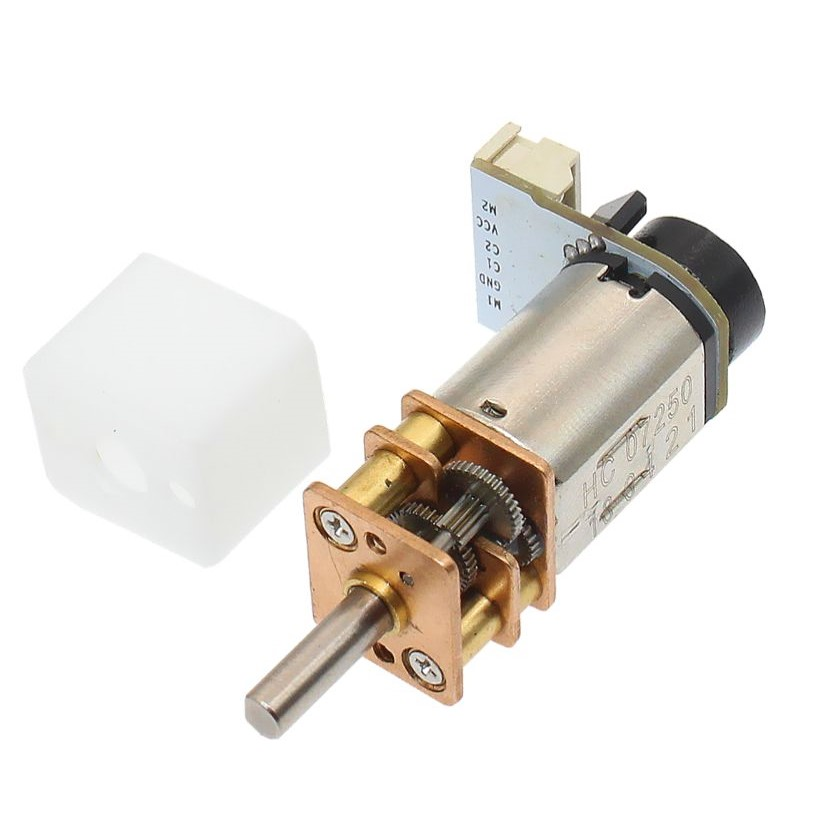
\includegraphics[height=5cm]{CHF-GM12-N20V.jpg}
      \caption{GW12-N20减速电机}
      \label{fig:GM12}
    \end{minipage}
\end{figure}

\section{三轮全向轮移动平台}
全向轮与麦克纳姆轮的共同点在于他们都由两大部分组成:轮毂和辊子(roller)。轮毂是整个轮子的主体支架,辊子则是安装在轮毂上的鼓状物。全向轮的轮毂轴与辊子转轴相互垂直,而麦克纳姆轮的轮毂轴与辊子转轴呈 45° 角。

经典的三轮全向轮(Omni Wheel)平台的全向轮中心平均分布在一个圆上。

\begin{equation}
    \left[\begin{array}{l}
    {V_{1}} \\
    {V_{2}} \\
    {V_{3}}
    \end{array}\right]=\left[\begin{array}{ccc}
    {-1} & {0} & {L} \\
    {\sin \frac{\pi}{6}} & {-\cos \frac{\pi}{6}} & {L} \\
    {\sin \frac{\pi}{6}} & {\cos \frac{\pi}{6}} & {L}
    \end{array}\right]\left[\begin{array}{l}
    {V_{x}} \\
    {V_{y}} \\
    {\omega}
    \end{array}\right]
\end{equation}

解算可得V1、V2、V3表达式:

\begin{equation}
    \left\{\begin{aligned}
    &V_{1}=-\frac{1}{2} V_{x}+\frac{\sqrt{3}}{2} V_{y}+L \omega \\
    &V_{2}=-\frac{1}{2} V_{x}-\frac{\sqrt{3}}{2} V_{y}+L \omega \\
    &V_{3}=V_{x}+L \omega
    \end{aligned}\right.
\end{equation}

\section{麦克纳姆轮}

\subsection{Mecanum wheel简介}
当需要车辆全向运动时,可以使用麦克纳姆轮(Mecanum wheel),如图~\ref{fig:Mecanum-wheel}。车辆可以沿着规定的路径移动,并同时绕其中心任意旋转,如图~\ref{fig:Vehicle-with-3-Mecanum-wheels}。麦克纳努姆轮由围绕轮轴排列的一组辊(roller)组成。

\begin{figure}
    \begin{minipage}{0.48\textwidth}
      \centering
      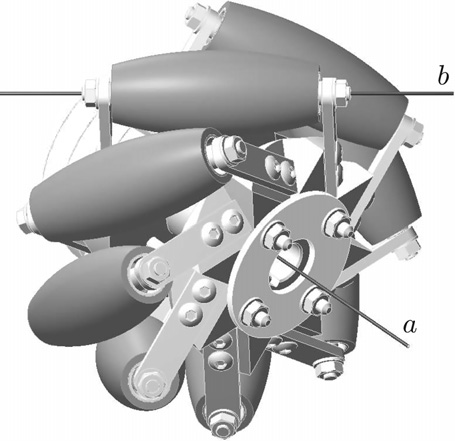
\includegraphics[height=5cm]{Mecanum-wheel.jpg}
      \caption{麦克纳姆轮}
      \label{fig:Mecanum-wheel}
    \end{minipage}\hfill
    \begin{minipage}{0.48\textwidth}
      \centering
      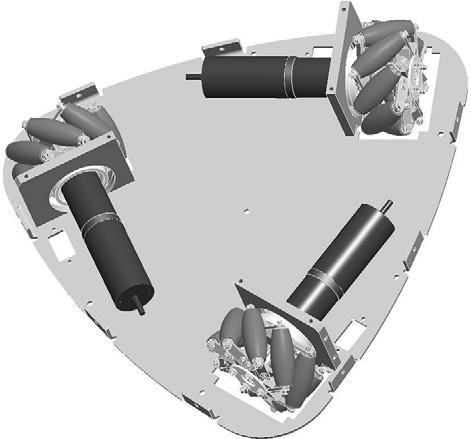
\includegraphics[height=5cm]{Vehicle-with-3-Mecanum-wheels.jpg}
      \caption{3麦克纳姆轮小车}
      \label{fig:Vehicle-with-3-Mecanum-wheels}
    \end{minipage}
\end{figure}

\subsection{Mecanum wheel几何描述}
为了使麦克纳姆轮能够在任意时刻都至少有一个辊子紧密接触地面,其几何学描述见图~\ref{fig:Curve-cR-generating-the-rolls}和图~\ref{fig:The-roll-surface-R},推导见Geometry and kinematics of the Mecanum wheel\cite{gfrerrer2008geometry}一文。

\begin{figure}[htbp]
    \centering
    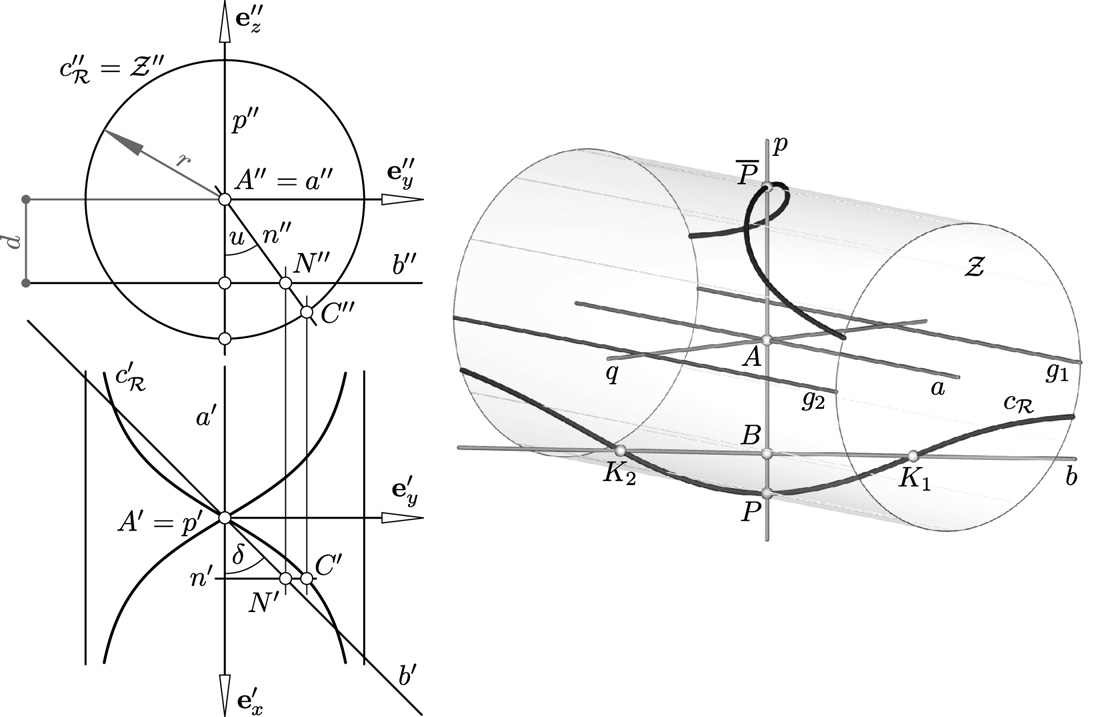
\includegraphics[height=10cm]{Curve-cR-generating-the-rolls.jpg}
    \caption{生成辊子曲面的曲线cR}
    \label{fig:Curve-cR-generating-the-rolls}
\end{figure}

\begin{figure}[htbp]
    \centering
    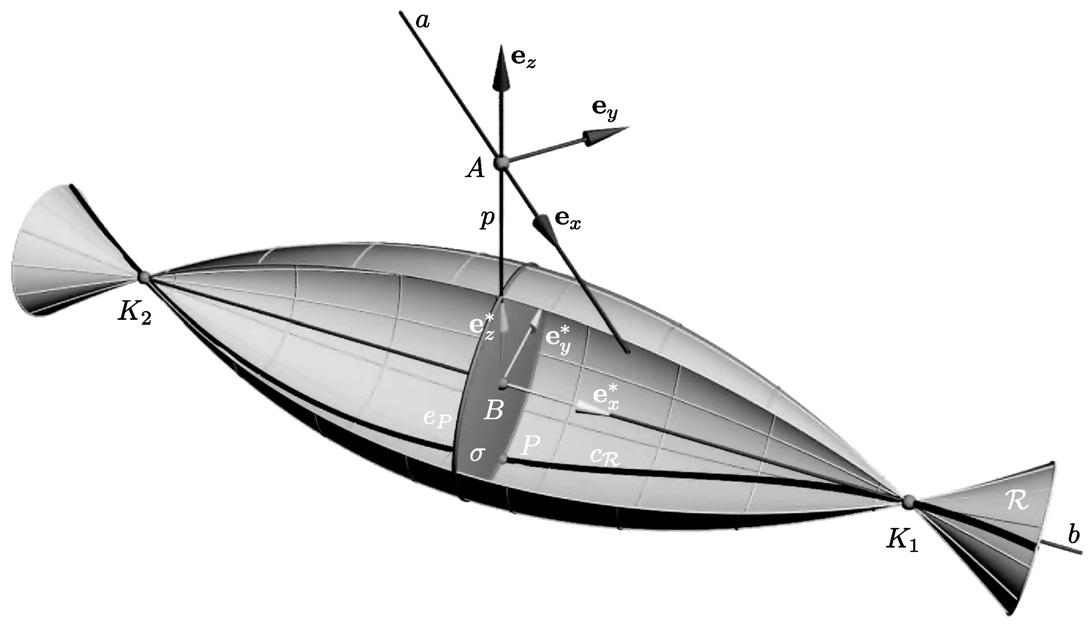
\includegraphics[height=8cm]{The-roll-surface-R.jpg}
    \caption{辊子曲面R}
    \label{fig:The-roll-surface-R}
\end{figure}

\subsection{Mecanum wheel动力学模型}

考虑一种装有麦克纳姆轮的车辆在水平地面上行驶,如图~\ref{fig:Vehicle-with-3-Mecanum-wheels}所示。分析某一时刻t(如图~\ref{fig:Velocities-Mecanum})上一个车轮的情况。

\begin{figure}[htbp]
    \centering
    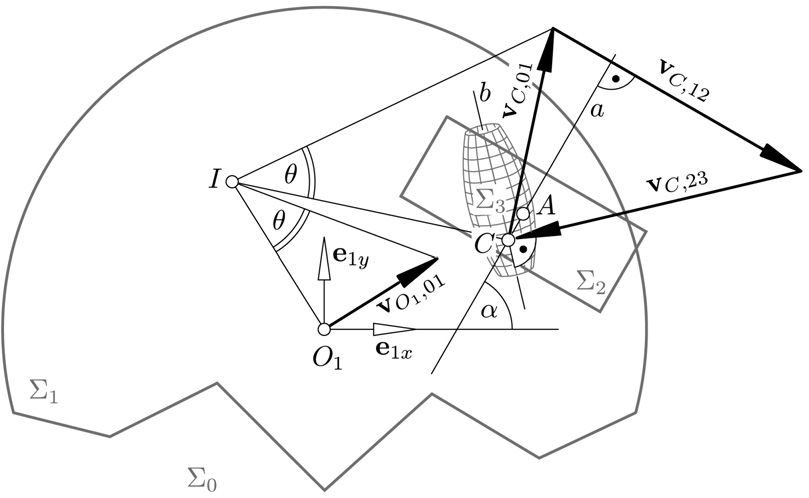
\includegraphics[height=10cm]{Velocities-Mecanum.jpg}
    \caption{麦克纳姆轮小车速度计算}
    \label{fig:Velocities-Mecanum}
\end{figure}

涉及四个系统:地面$\Sigma_{0}$,车$\Sigma_{1}$,车轮$\Sigma_{2}$和辊子$\Sigma_{3}$,这时在点C(接触点)接触地面。注意,该点始终位于车轮$\Sigma_{2}$的轴a之下:它是车轮转轴a和辊子转轴b在$\Sigma_{0}$中的正交投影的交点。仅在b处于水平位置的情况下,C才位于车轮中心A下方!

为了进行分析描述,我们选择$\Sigma_{1}$中的任意点$O_{1}$(“车辆中心 vehicle center”)作为坐标系$S_{1}:=\left\{O_{1} ; \mathbf{e}_{1 x}, \mathbf{e}_{1 y}, \mathbf{e}_{1 z}\right\}$的原点,与$\Sigma_{1}$相切,x和y轴平行于地面。车轮中心A可能有x和y坐标$a_x$和$a_y$。考虑到$S_1$和α可以表示$\mathbf{e}_{1 x}$与车轮轴线a之间的角度,则:

\begin{equation}
    \mathbf{a}=\left(\begin{array}{c}
    {\cos \alpha} \\
    {\sin \alpha} \\
    {0}
    \end{array}\right)
\end{equation}

是a轴的方向向量,辊子转轴的方向向量b取决于车轮的旋转角度u:

\begin{equation}
    \mathbf{b}=\left(\begin{array}{c}
    {\cos \alpha \cos \delta-\sin \alpha \sin \delta \cos u} \\
    {\sin \alpha \cos \delta+\cos \alpha \sin \delta \cos u} \\
    {\sin \delta \sin u}
    \end{array}\right)=:\left(\begin{array}{l}
    {b_{x}} \\
    {b_{y}} \\
    {b_{z}}
    \end{array}\right)
\end{equation}

在$S_1$坐标系中,接触点C的x和y坐标为:

\begin{equation}
    \left.\begin{array}{l}
    {c_{x}=a_{x}-d \cos \alpha \cot \delta \tan u} \\
    {c_{y}=a_{y}-d \sin \alpha \cot \delta \tan u}
    \end{array}\right\}
\end{equation}


在以下考虑中,我们可以忽略$z$-轴,因为出现的速度矢量都与$x y$平面平行。

在$t$时刻,令 $\omega$ 为 $\Sigma_{1} / \Sigma_{0}$ (vehicle/ground)运动的速度向量,$\mathbf{v}_{O_{1}, 01}=\left(v_{x}, v_{y}\right)^{\top}$ 为 $O_{1}$ 的速度向量。对于$\Sigma_{1} / \Sigma_{0}$相对运动,接触点C的速度向量为:

\begin{equation}
\mathbf{v}_{C, 01}=\left(\begin{array}{c}
{v_{x}-\omega c_{y}} \\
{v_{y}+\omega c_{x}}
\end{array}\right)
\end{equation}

$\Sigma_{2} / \Sigma_{1}$ (wheel/vehicle) 相对运动是绕轴a的简单旋转,因此,该相对运动C的速度矢量为


\begin{equation}
    \mathbf{v}_{C, 12}=\dot{u} r\left(\begin{array}{c}
    {-\sin \alpha} \\
    {\cos \alpha}
    \end{array}\right)
\end{equation}

其中 $\dot{u}=\frac{d u}{d t}$ 是 $\Sigma_{2} / \Sigma_{1}$ 的角速度。

$\Sigma_{3} / \Sigma_{2}$ (roll/wheel) 是绕$b$的旋转,因此,$C$的瞬时矢量速度 $\mathbf{v}_{\mathrm{C}, 23}$ 是垂直于 $\mathbf{b}$ 的:

\begin{equation}
\mathbf{v}_{C, 23}=\lambda\left(\begin{array}{c}
{-b_{y}} \\
{b_{x}}
\end{array}\right)
\end{equation}

因为辊子(被动)在地面上不滑动,$\Sigma_{3} / \Sigma_{0}$(roll/ground)的C速度$\mathbf{v}_{\mathrm{C}, 03}$必须为零。根据速度叠加原理,我们得到:

\begin{equation}
    \mathbf{v}_{C, 01}+\mathbf{v}_{C, 12}+\mathbf{v}_{C, 23}=\mathbf{v}_{C, 03}=\mathbf{o}=(0,0)^{\top}
\end{equation}

综上:

\begin{equation}
    \left.\begin{array}{l}
    {r \sin \alpha \dot{u}+b_{y} \lambda=v_{x}-\omega c_{y}} \\
    {r \cos \alpha \dot{u}+b_{x} \lambda=-v_{y}-\omega c_{x}}
    \end{array}\right\}
\end{equation}

通过消去λ得到微分方程:

\begin{equation}
    r\left(b_{x} \sin \alpha-b_{y} \cos \alpha\right) \dot{u}-b_{x}\left(v_{x}-\omega c_{y}\right)-b_{y}\left(v_{y}+\omega c_{x}\right)=0
\end{equation}

代入经简化的初始条件 $b_{x}=\cos (\alpha+\delta), b_{y}=\sin (\alpha+\delta), c_{x}=a_{x}, c_{y}=a_{y}$ 得:

\begin{equation}
    \label{eq:u}
    \dot{u}=-\frac{1}{r \sin \delta}\left[\sin (\alpha+\delta)\left(v_{y}+\omega a_{x}\right)+\cos (\alpha+\delta)\left(v_{x}-\omega a_{y}\right)\right]
\end{equation}

给定车速数据 $v_{x}, v_{y}, \omega$,该公式可以计算(近似)车轮转速$\dot{u}$。

\subsection{三麦克纳姆轮系统运动控制}

研究一个装有三个Mecanum轮,车轮中心为$A_{i}\left(a_{i x}, a_{i y}\right)$,主动轮轮轴角$\alpha_{i}, i=1,2,3$,子轮角度是$\delta$的小车,如果我们用$\omega_i$表示每个车轮的角速度,则根据等式~\ref{eq:u}我们有:

\begin{equation}
    \label{eq:inverse}
    \left(\begin{array}{l}
    {\omega_{1}} \\
    {\omega_{2}} \\
    {\omega_{3}}
    \end{array}\right)=-\frac{1}{r \sin \delta} \mathbf{M}\left(\begin{array}{c}
    {v_{x}} \\
    {v_{y}} \\
    {\omega}
    \end{array}\right)
\end{equation}

其中:

\begin{equation}
    \mathbf{M}=\left(\begin{array}{ccc}
    {\cos \left(\alpha_{1}+\delta\right)} & {\sin \left(\alpha_{1}+\delta\right)} & {a_{1 x} \sin \left(\alpha_{1}+\delta\right)-a_{1 y} \cos \left(\alpha_{1}+\delta\right)} \\
    {\cos \left(\alpha_{2}+\delta\right)} & {\sin \left(\alpha_{2}+\delta\right)} & {a_{2 x} \sin \left(\alpha_{2}+\delta\right)-a_{2 y} \cos \left(\alpha_{2}+\delta\right)} \\
    {\cos \left(\alpha_{3}+\delta\right)} & {\sin \left(\alpha_{3}+\delta\right)} & {a_{3 x} \sin \left(\alpha_{3}+\delta\right)-a_{3 y} \cos \left(\alpha_{3}+\delta\right)}
    \end{array}\right)
\end{equation}

式~\ref{eq:inverse}是车辆逆运动学问题的解。

在本问题的情境下:

\begin{definition}
    逆运动学问题:给定小车速度和转动角速度,求三个轮子各自的转速。
\end{definition}

\begin{definition}
    正运动学问题:给定三个轮子各自的转速,求小车速度和转动角速度。
\end{definition}

显然,当且仅当$\operatorname{det} \mathbf{M} \neq 0$,正运动学问题存在唯一解

\begin{equation}
    \left(\begin{array}{c}
    {v_{x}} \\
    {v_{y}} \\
    {\omega}
    \end{array}\right)=-r \sin \delta \mathbf{M}^{-1}\left(\begin{array}{c}
    {\omega_{1}} \\
    {\omega_{2}} \\
    {\omega_{3}}
    \end{array}\right)
\end{equation}

\begin{theorem}\label{the:theorem-en}
    The direct kinematics of a robot with three Mecanum wheels has a unique solution if and only if the wheels are arranged so that the roll axes are not concurrent or parallel.\hfill —— A. Gfrerrer
\end{theorem}

即:

\begin{theorem}\label{the:theorem-cn}
    当且仅当车轮排布使得小轮不平行时,3-Mecanum轮机器人才具有运动学唯一解。
\end{theorem}


\chapter{动力系统}
\label{cha:Motor}

注:微型反折步进电机和38mm全向轮之间联轴器上的螺丝配的是M3*4的圆头螺钉,在电机旋转时会碰到电机机身卡住,故换成M3*3的PM圆头螺丝。

\section{步进电机概述和控制理论}

\footnote{参考\url{https://www.moons.com.cn/support-training/technology-college/cn-stepper-motor}}

步进电机是将电脉冲信号转变为角位移或线位移的开环控制元步进电机件,通过控制施加在电机线圈上的电脉冲顺序、频率和数量,可以实现对步进电机的转向、速度和旋转角度的控制。配合以直线运动执行机构或齿轮箱装置,更可以实现更加复杂、精密的线性运动控制要求。步进电机一般由前后端盖、轴承、中心轴、转子铁芯、定子铁芯、定子组件、波纹垫圈、螺钉等部分构成,步进电机也叫步进器,它利用电磁学原理,将电能转换为机械能,是由缠绕在电机定子齿槽上的线圈驱动的。通常情况下,一根绕成圈状的金属丝叫做螺线管,而在电机中,绕在定子齿槽上的金属丝则叫做绕组、线圈、或相。如图~\ref{fig:Stepper-Motor-Open}。

\begin{figure}[htbp]
    \centering
    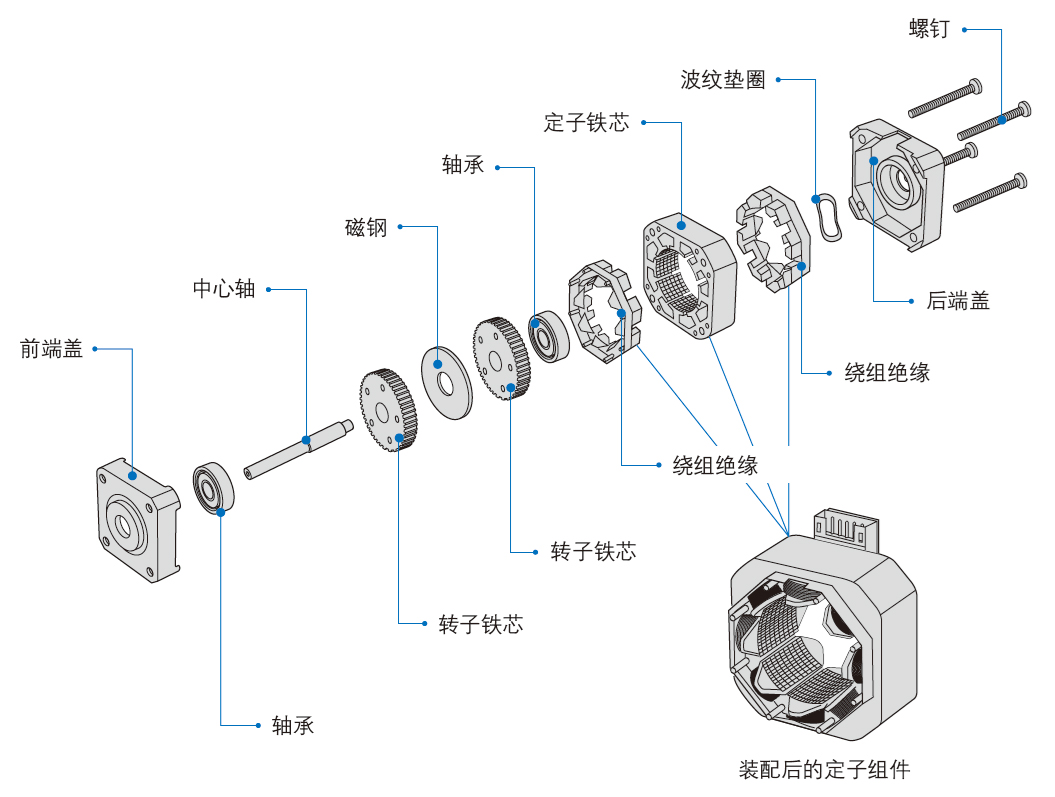
\includegraphics[width=\columnwidth]{step-servo-motord01.jpg}
    \caption{步进电机基本结构}
    \label{fig:Stepper-Motor-Open}
\end{figure}

步进电机驱动器根据外来的控制脉冲和方向信号,通过其内部的逻辑电路,控制步进电机的绕组以一定的时序正向或反向通电, 使得电机正向/反向旋转,或者锁定。

以1.8度两相步进电机为例:当两相绕组都通电励磁时,电机输出轴将静止并锁定位置。在额定电流下使电机保持锁定的最大力矩为保持力矩。如果其中一相绕组的电流发生了变向,则电机将顺着一个既定方向旋转一步(1.8度)。同理,如果是另外一项绕 组的电流发生了变向,则电机将顺着与前者相反的方向旋转一步(1.8度)。当通过线圈绕组的电流按顺序依次变向励磁时,则电 机会顺着既定的方向实现连续旋转步进,运行精度非常高。对于 1.8度两相步进电机旋转一周需200步。

两相步进电机有两种绕组形式:双极性和单极性。双极性电机每相上只有一个绕组线圈,电机连续旋转时电流要在 同一线圈内依次变向励磁,驱动电路设计上需要八个电子开关进 行顺序切换。

单极性电机每相上有两个极性相反的绕组线圈,如图~\ref{fig:bipolar},电机连续旋转时只要交替对同一相上的两个绕组线圈进行通电励磁。驱动电路设 计上只需要四个电子开关。在双极性驱动模式下,如图~\ref{fig:unipolar},因为每相的绕组线圈为100\%励磁,所以双极性驱动模式下电机的输出力矩比单极性驱动模式下提高了约 40\%。

\begin{figure}[htbp]
    \begin{minipage}{0.48\textwidth}
      \centering
      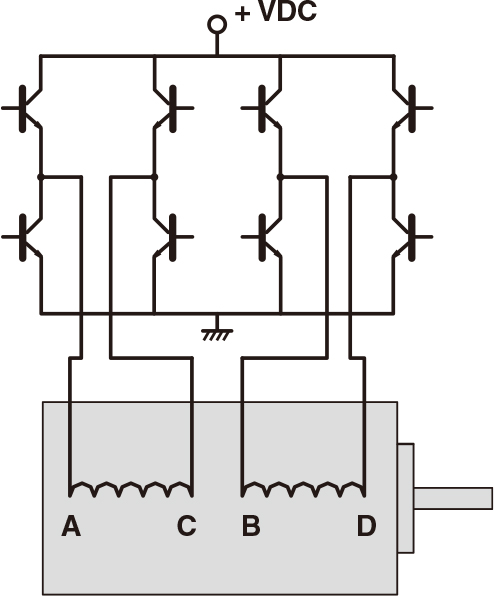
\includegraphics[height=5cm]{step-motor-2-phase-with-bipolar-driver.jpg}
      \caption{2相(双极性)步进电机}
      \label{fig:bipolar}
    \end{minipage}\hfill
    \begin{minipage}{0.48\textwidth}
      \centering
      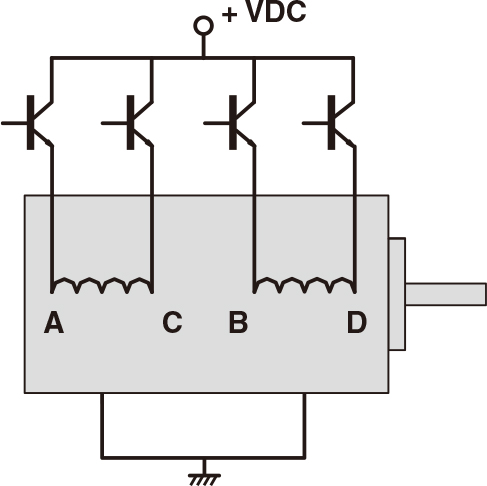
\includegraphics[height=5cm]{step-motor-2-phase-with-unipolar-driver.jpg}
      \caption{2相(单极性)步进电机}
      \label{fig:unipolar}
    \end{minipage}
\end{figure}


\section{步进电机转矩和速度特性}

步进电机的转动距离正比于施加到驱动器上的脉冲信号数(脉冲数)。

步进电机转动(电机出力轴转动角度$\theta$)和脉冲数A的关系如下所示:

\begin{equation}
    \theta=\theta_{s} \times A
\end{equation}

其中$\theta_{s}$为基本步距角,单位是度。

步进电机以一个固定的步距角转动,就像时钟内的秒针。这个角度称为基本步距角。一种标准电机是基本步距角为1.8度的两相步进电机。

步进电机的转速与施加到驱动器上的脉冲信号频率成比例关系。

电机的转速$\mathrm{N}$[r/min] 与脉冲频率$\mathrm{f}$[Hz] 的关系如下(整步模式):

\begin{equation}
    \mathrm{N}=\frac{\theta_{\mathrm{s}}}{360} \times \mathrm{f} \times 60
\end{equation}

步进电机的重要特征之一是高力矩、小体积。如图~\ref{fig:step-servo-motord}。

\begin{figure}[htbp]
    \centering
    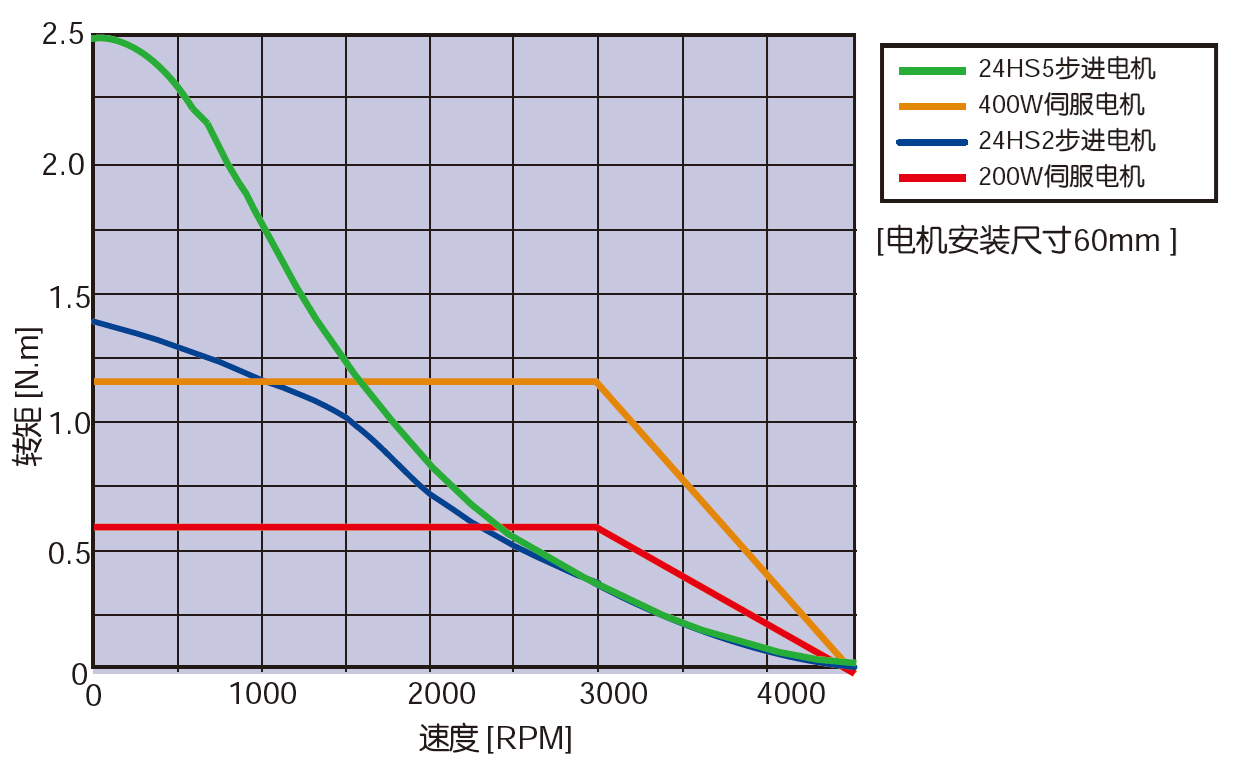
\includegraphics[width=\columnwidth]{step-servo-motord.jpg}
    \caption{相同尺寸下的伺服电机与步进电机的速度力矩特性比较}
    \label{fig:step-servo-motord}
\end{figure}

这些特征使得电机具有优秀的加速和响应,使得这些电机非常适合那些需要频繁启动和停止的应用中。

绕组通电时步进电机具有全部的保持力矩。这就意味着步进电机可以在不使用机械刹车的情况下保持在停止位置。

步进电机的输出力矩随转速升高而下降,且在较高转速时会急剧下降,所以其最高工作转速一般在300~600RPM。

静力矩是选择步进电机的主要参数之一,在判断需要多大的静力矩时要保证步进电机的输出转矩大于负载所需的转矩,这样才能保证整个系统的正常运转,而负载可分为惯性负载和摩擦负载两种。单一的惯性负载和单一的摩擦负载是不存在的。直接启动时两种负载均要考虑,加速启动时主要考虑惯性负载,恒速运行时只要考虑摩擦负载。在计算整个机械系统的负载转矩时,电机的矩频特性能满足机械负载并有一定的余量保证其可靠运行(步进电机的安全系数一般选择1.3~2)。在实际工作过程中,各种频率下的负载转矩必须在矩频特性曲线的范围内,一般来说,静力矩越大的电机,输出转矩也越大,承受负载能力越强。

速度-力矩曲线(图~\ref{fig:step-motor-force})是步进电机输出特性的重要表现形式。

\begin{figure}[htbp]
    \centering
    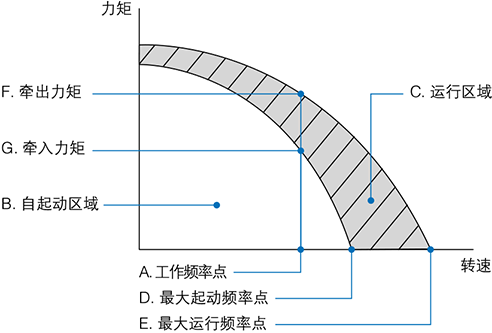
\includegraphics[width=\columnwidth]{step-motor-force.png}
    \caption{速度-力矩曲线}
    \label{fig:step-motor-force}
\end{figure}

A. 工作频率点 电机在某一点的转速值。

速率:

n = q * Hz / (360 * D)

n: 转/秒

Hz: 频率值

D: 驱动电路细分值

q: 步距角

步距角1.8°的步进电机,在 1/2 细分驱动方式下 (即每步 0.9°) 、 工作频率 500Hz 时的转速为1.25r/s.

B. 自启动区域: 步进电机可以直接启动和停止的区域。

C. 连续运行区域: 在该区域内,电机无法直接启动或停止。电机在该区域内运行必须先经过自启动区域,然后经 过加速达到该工作区域运行。同理,电机在该区域内也无法直接制动,否则容易造成电机失步, 必须先经过减速到达自启动区域内再制动。

D. 最高启动频率: 空载情况下,已励磁电机直接启动而不丢步的最高脉冲频率。

E. 最高运行频率: 空载情况下,已励磁电机运行而不丢步的最高脉冲频率。

F. 启动力矩/牵入力矩: 已励磁电机能以某一固定的频率启动和同步运行而不丢步的最大转矩。

G. 运行力矩/牵出力矩: 在规定的驱动条件下,按照给定脉冲频率,可加给已驱动电机转轴上而不是电机丢步的最大转矩。

\section{单极性驱动和双极性驱动的区别}

双极步进电机(Bipolar motors\footnote{\url{https://en.wikipedia.org/wiki/Stepper_motor}})每相只有一个绕组。为了使磁极反向,需要使绕组中的电流反向,因此驱动电路必须更复杂,通常采用H桥配置(但是有几种现成的驱动器芯片可以使之成为一个简单的事情)。每相有两个引线,没有公用的。

两线圈双极步进步进电机的典型驱动模式为:A + B + A- B-。即以正电流驱动线圈A,然后从线圈A中去除电流。然后以正电流驱动线圈B,然后从线圈B中去除电流。然后用负电流驱动线圈A(通过切换导线,例如用H桥翻转极性),然后从线圈A去除电流。然后用负电流驱动线圈B(与线圈A的翻转极性相同);循环完成并重新开始。

由于更好地利用了绕组,因此它们比同等重量的单极步进电机更强大。这是由于绕组占用的物理空间。单极电机在相同的空间中具有两倍的导线数量,但在任何时间点仅使用一半的导线,因此效率为50\%(或大约70\%的可用扭矩输出)。尽管双极步进电机的驱动更加复杂,但丰富的驱动芯片简化了实际使用时的复杂度。

单极性 (unipolar) 和双极性 (bipolar) 是步进电机最常采用的两种驱动电路。单极性驱动电路使用四颗晶体管来驱动步进电机的两组相位,电机定子绕线结构如图~\ref{fig:step-motor-unibipolar}所示包含两组带有中间抽头的线圈(AC线圈的中间抽头为O,BD线圈的中间抽头为M),整个电机共有六条线与外界连接。AC端不能同时通电(BD端同理),否则磁极上的两个线圈产生的磁通相互抵消,只产生线圈的铜耗。因为它其实只有两个相位(AC绕组为一相,BD绕组为一相),准确的说法应是两相六线式步进电机。

\begin{figure}[htbp]
    \centering
    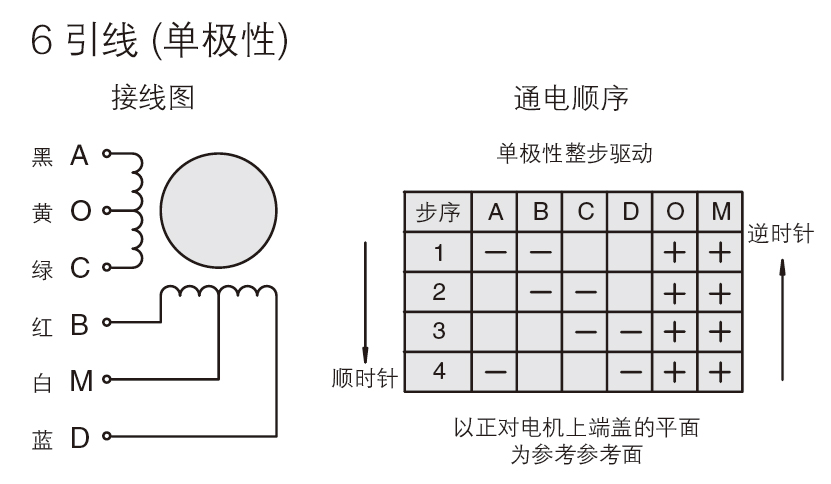
\includegraphics[width=\columnwidth]{step-motor-unibipolar.jpg}
    \caption{单极性驱动电路}
    \label{fig:step-motor-unibipolar}
\end{figure}

双极性步进电机的驱动电路则如图~\ref{fig:step-motor-unibipolar-2}所示,它使用八颗晶体管来驱动两组相位。定子磁极的线圈为单线圈绕组,通过切换线圈AC和线圈BD的的电流方向来切换磁极的正反方向。步进电机的发展初期由于受到晶体管半导体原件的成本影响,单极性电机由于其控制电路使用的晶体管数量少而得到一定范围的应用,但是随着上世纪五六十年代半导体材料的高速发展,晶体管成本大大降低,双极性电机凭借着性能上的优势使其使用量急剧增加。

\begin{figure}[htbp]
    \centering
    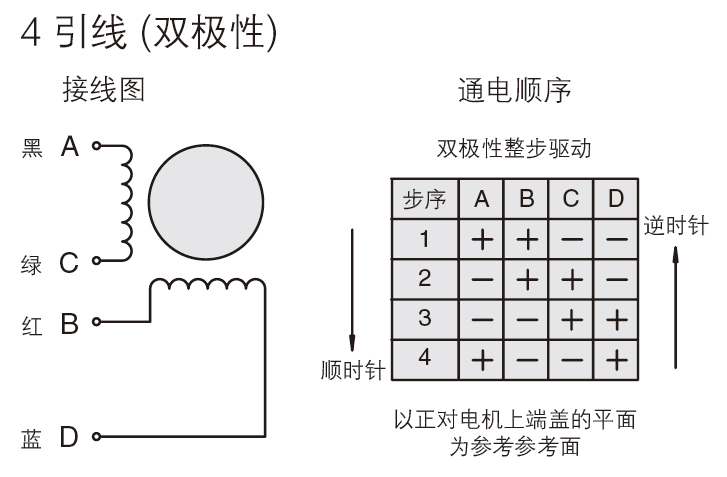
\includegraphics[width=\columnwidth]{step-motor-unibipolar-2.jpg}
    \caption{双极性驱动电路}
    \label{fig:step-motor-unibipolar-2}
\end{figure}

图~\ref{fig:step-motor-unibipolar-3}所示的是单极性与双极性两种绕线方式,导线线径相同时,单极方式的线圈绕组匝数为N,电阻为R,双极方式的线圈绕组匝数为2N,线圈电阻则为2R。

\begin{figure}[htbp]
    \centering
    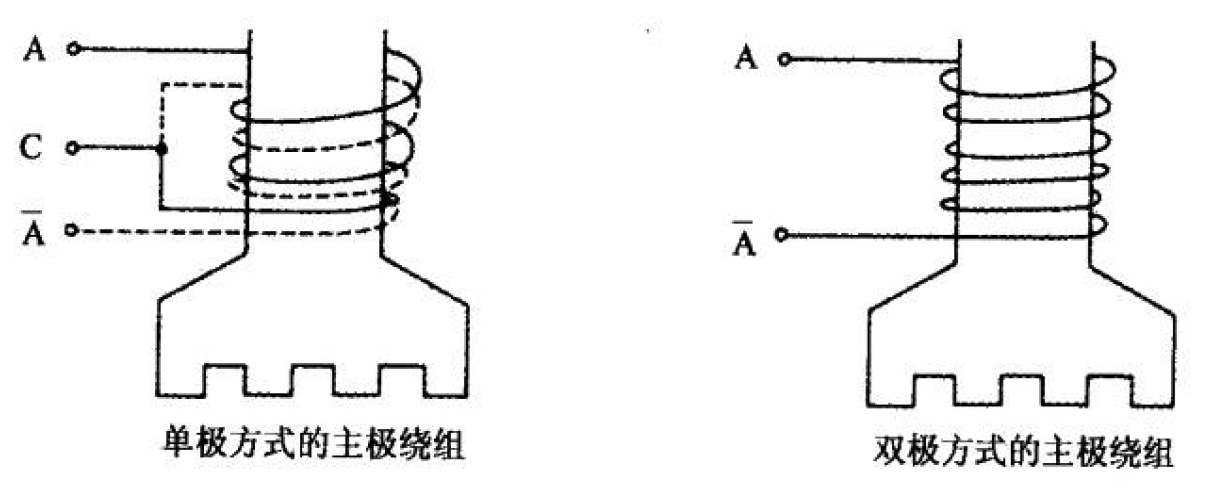
\includegraphics[width=\columnwidth]{step-motor-unibipolar-3.jpg}
    \caption{单极性与双极性绕组}
    \label{fig:step-motor-unibipolar-3}
\end{figure}

表~\ref{tab:step-motor-unibipolar}所示恒压驱动电路在低速时,单极与双极驱动工作效率的对比。电流与线圈匝数的乘积称为安匝数,与转矩成正比,如果两者转速相同,输出功率与安匝数有比例关系。同样,双极性电流为V/2R,匝数也为2N,乘积的结果与单极性同为VN/R。输入恒压驱动的情形,单极性与双极性比较,如表~\ref{tab:step-motor-unibipolar}所示,电流只有单极性的二分之一,低速时的效率为单极性的2倍。

\begin{table}[htbp]
    \centering
    \begin{tabular}{lll}
     & 单极性 & 双极性 \\
    安匝数 & $U_{1}=V \times \frac{N}{R}$ & $U_{2}=V \times \frac{2N}{2R}=V \times \frac{N}{R}$\\
    输入功率 & $W_{1}=\frac{\mathrm{V}^{2}}{R}$ & $\mathrm{W}_{2}=(\frac{\mathrm{V}}{2 \mathrm{R}} )^{2} \times  2 \mathrm{R}=\frac{\mathrm{V}^{2}}{2 \mathrm{R}} $ \\
    效率 & $\eta = \frac{U_{1}}{W_{1}} = \frac{N}{V}$ & $\eta = \frac{U_{2}}{W_{2}} = \frac{2N}{V}$
    \end{tabular}
    \caption{单极驱动与双极驱动效率对比 注:V为所加电压;R为电机线圈电阻;N为单极匝数}
    \label{tab:step-motor-unibipolar}
\end{table}

所以小型化或低速应用时,有大转矩需求,应使用双极性电机及驱动。高速应用的情况下,因为双极性电机匝数多,电感变大,反电势增大,使高速时电流减少,从而降低转矩,所以需要注意与单极性的转矩比较。

图~\ref{fig:step-motor-unibipolar-4}为单极性步进电机与双极性步进电机的特性曲线,均采用同一恒流驱动方式。一般低速大转矩的负载应用使用双极性驱动,而高速驱动应用以单极性驱动较为合适。

\begin{figure}[htbp]
    \centering
    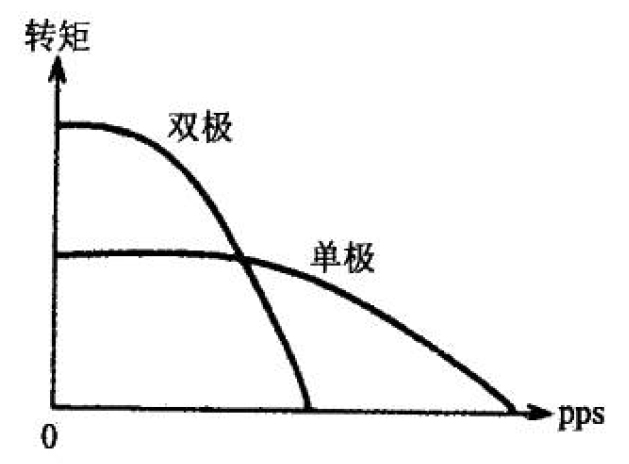
\includegraphics[width=0.5\columnwidth]{step-motor-unibipolar-4.jpg}
    \caption{单极驱动与双极驱动的矩频曲线对比}
    \label{fig:step-motor-unibipolar-4}
\end{figure}

\section{步进电机驱动}

斩波驱动电路(Chopper drive circuits)称为受控电流驱动器,因为它们在每个绕组中产生受控电流,而不是施加恒定电压。斩波器驱动电路最常用于双绕组双极步进电机,两个绕组被独立驱动以提供特定的步进电机转矩CW或CCW。在每个绕组上,将“电源”电压作为方波电压施加到绕组上。例如8 kHz。绕组电感使电流平滑,该电流达到根据方波占空比的水平。相对于绕组回路,双极性电源(+和-)电压通常提供给控制器。

如图~\ref{fig:Phase-current}

\begin{figure}[htbp]
    \centering
    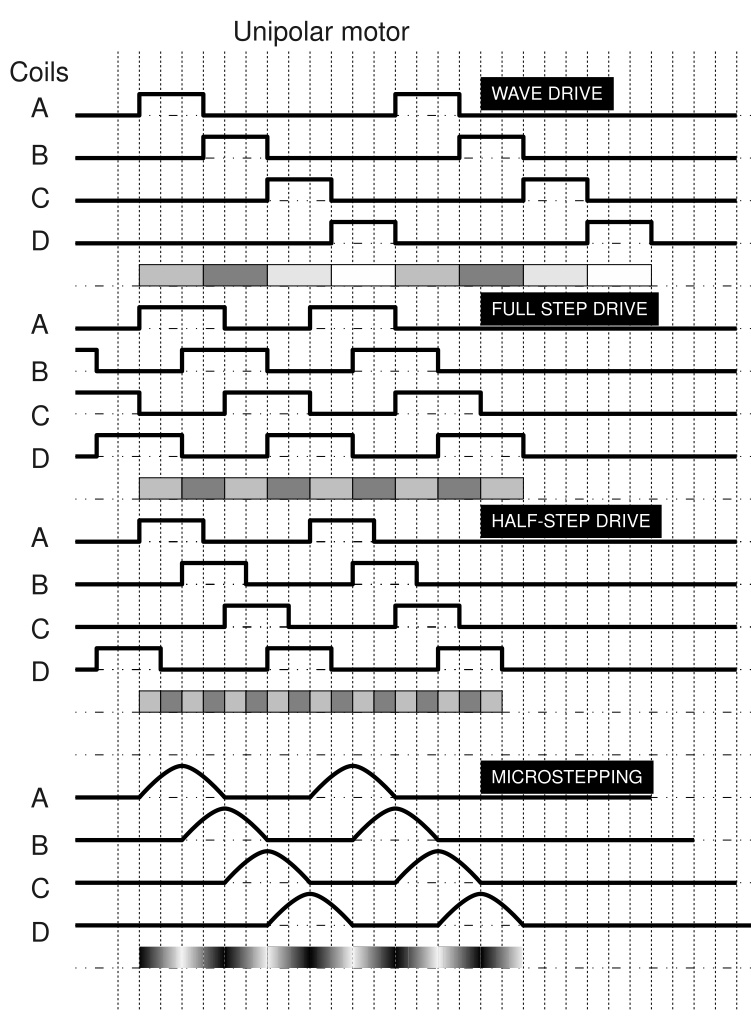
\includegraphics[width=\columnwidth]{Drive.png}
    \caption{Phase current waveforms}
    \label{fig:Phase-current}
\end{figure}

\section{步进电机驱动DRV8825}

DRV8825用于双极步进电机控制。微步步进电机驱动器提供更高的精度以及步进电机平稳的旋转。

\begin{figure}[htbp]
    \centering
    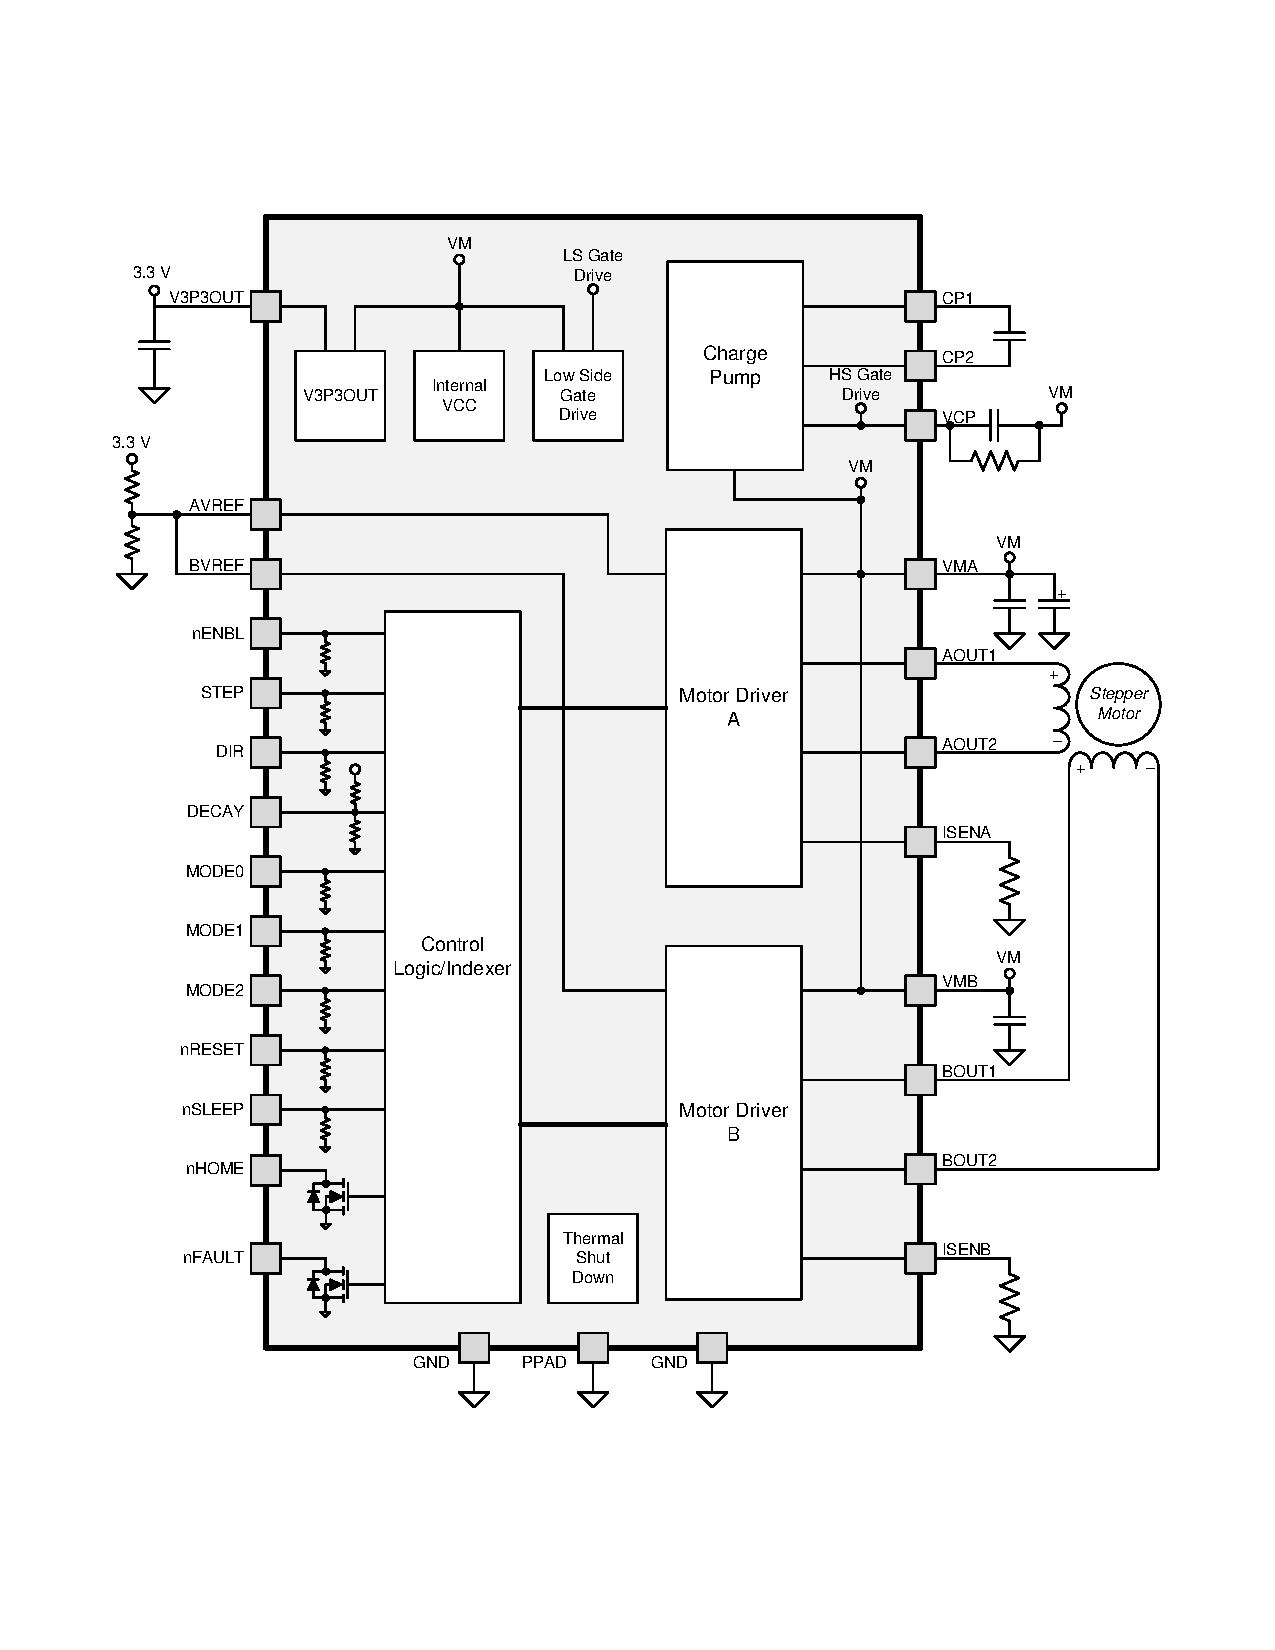
\includegraphics[width=\columnwidth]{DRV8825-Function-Block.pdf}
    \caption{DRV8825功能框图}
    \label{fig:DRV8825-Function-Block}
\end{figure}

配置DRV8825的第一步需要所需的转速和微步级别。

\begin{figure}[htbp]
    \centering
    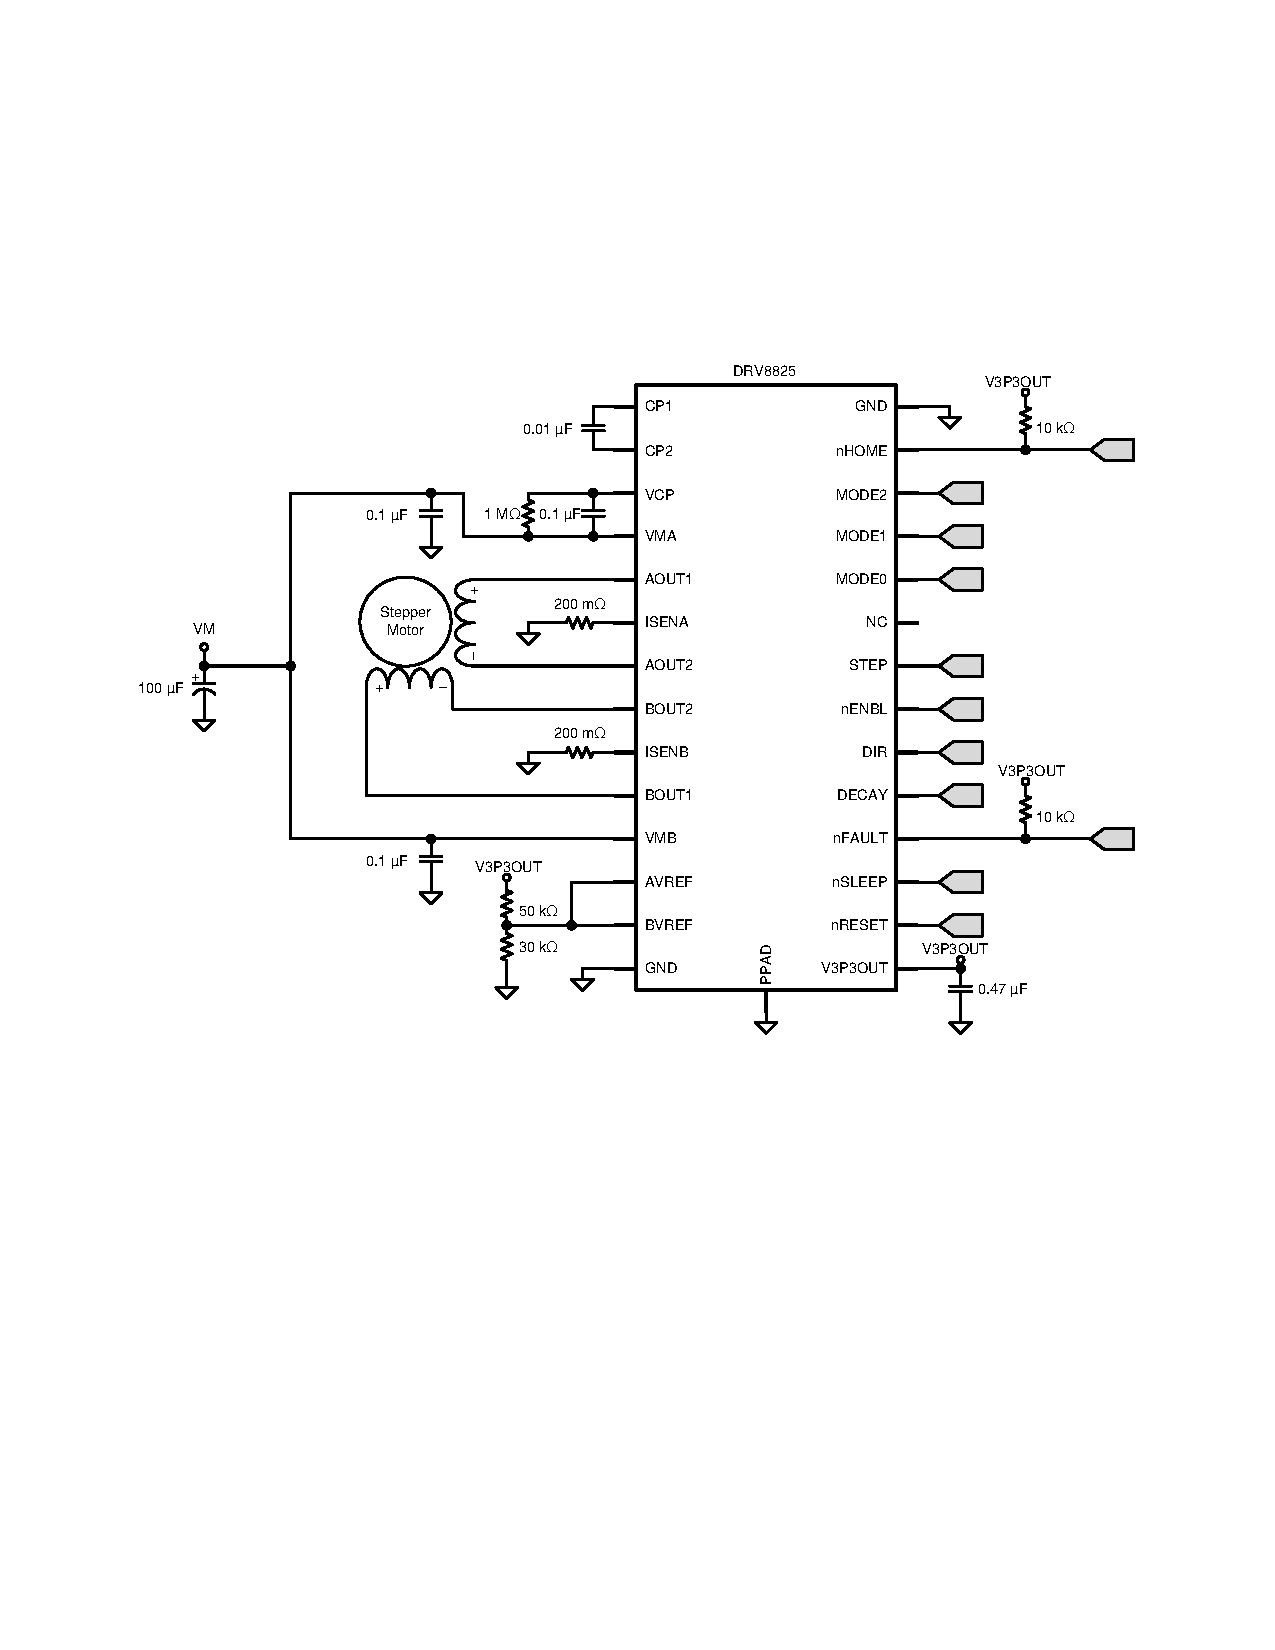
\includegraphics[width=\columnwidth]{DRV8825-Typical-Application.pdf}
    \caption{DRV8825典型应用}
    \label{fig:DRV8825-Typical-Application}
\end{figure}


\begin{figure}[htbp]
    \centering
    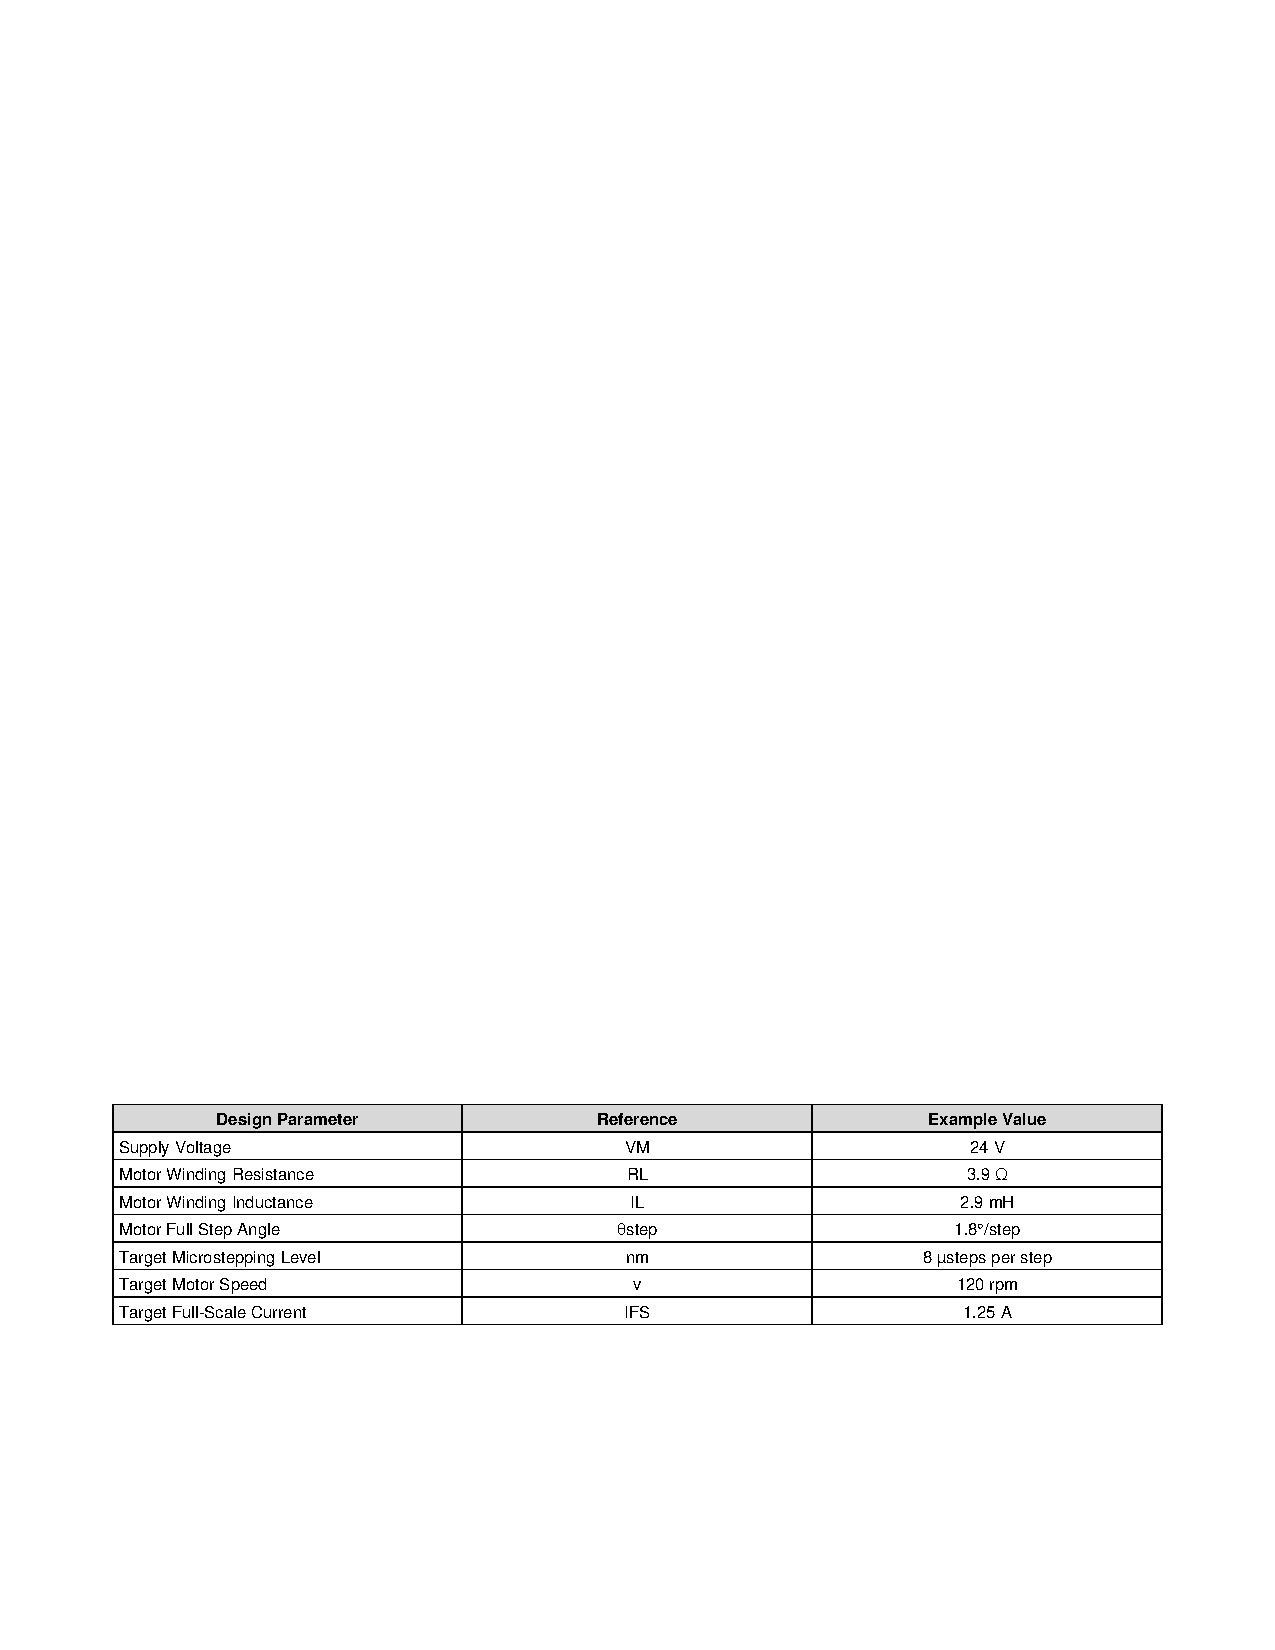
\includegraphics[width=\columnwidth]{DRV8825-Design-Requirements.pdf}
    \caption{DRV8825设计要求}
    \label{fig:DRV8825-Design-Requirements}
\end{figure}

如果需要恒定转速,则将频率为$f_step$的方波施加到STEP引脚。

如果步进电机的目标速度过高,步进电机可能不会旋转。 确保步进电机可以支持目标速度或通过加速以使步进电机达到最高速度。

对于所需的步进电机速度(v),微步级别($n_m$)和步进电机全步距角($\theta_{\text {step }}$,一整步对应的角度),

\begin{equation}
    \begin{aligned}
    &f_{\text {step }(\mu \text { steps } / \text { second })=} \frac{v\left(\frac{\text { rotations }}{\text { minute }}\right) \times 360\left(\frac{\circ}{\text { rotation }}\right) \times n_{\mathrm{m}}\left(\frac{\mu \text { steps }}{\text { step }}\right)}{60\left(\frac{\text { seconds }}{\text { minute }}\right) \times \theta_{\text {step }}\left(\frac{^{\circ}}{\text { step }}\right)}\\
    &f_{\text {step }(\mu \text { steps } / \text { second })=} \frac{120\left(\frac{\text { rotations }}{\text { minute }}\right) \times 360\left(\frac{^{\circ}}{\text { rotation }}\right) \times 8\left(\frac{\mu \text { steps }}{\text { step }}\right)}{60\left(\frac{\text { seconds }}{\text { minute }}\right) \times 1.8\left(\frac{\circ}{\text { step }}\right)}
    \end{aligned}
\end{equation}

DRV8825微步步进级别由MODE引脚设置,如表~\ref{tab:DRV8825-microstep-settings}所示。

\begin{table}[htbp]
    \centering
    \begin{tabular}{llll}
    \hline
    M0   & M1   & M2   & Microstep resolution \\ \hline
    Low  & Low  & Low  & Full step            \\ \hline
    High & Low  & Low  & 1/2 step             \\ \hline
    Low  & High & Low  & 1/4 step             \\ \hline
    High & High & Low  & 1/8 step             \\ \hline
    Low  & Low  & High & 1/16 step            \\ \hline
    High & Low  & High & 1/32 step            \\ \hline
    Low  & High & High & 1/32 step            \\ \hline
    High & High & High & 1/32 step            \\ \hline
    \end{tabular}
    \caption{DRV8825 microstep settings}
    \label{tab:DRV8825-microstep-settings}
\end{table}

较高的微步步进级别将意味着步进电机运动更平稳且噪声较小,但会增加开关损耗,并且需要较高的$f_step$才能达到相同的步进电机速度。

在步进电机中,设定的满量程电流($I_{FS}$ full-scale current)是通过任一绕组驱动的最大电流。 该数量取决于xVREF模拟电压和检测电阻值($R_{\text {SENSE}}$)。 

在步进期间,IFS定义为最大电流步进斩波阈值($I_{\text {TRIP}}$ current chopping threshold)。 DRV8825的增益设置为5V。

\begin{equation}
    \operatorname{I_{FS}}(A)=\frac{x \operatorname{VREF}(V)}{A_{v} \times R_{S E N S E}(\Omega)}=\frac{x \operatorname{VREF}(V)}{5 \times R_{S E N S E}(\Omega)}
\end{equation}

参考设计和要求如图~\ref{fig:DRV8825-Typical-Application}和图~\ref{fig:DRV8825-Design-Requirements}

典型模块设计和布局如图~\ref{fig:DRV8825-stepper-motor-driver-carrier-schematic-diagram}和图~\ref{fig:DRV8825-Layout-Example}

\begin{figure}[htbp]
    \centering
    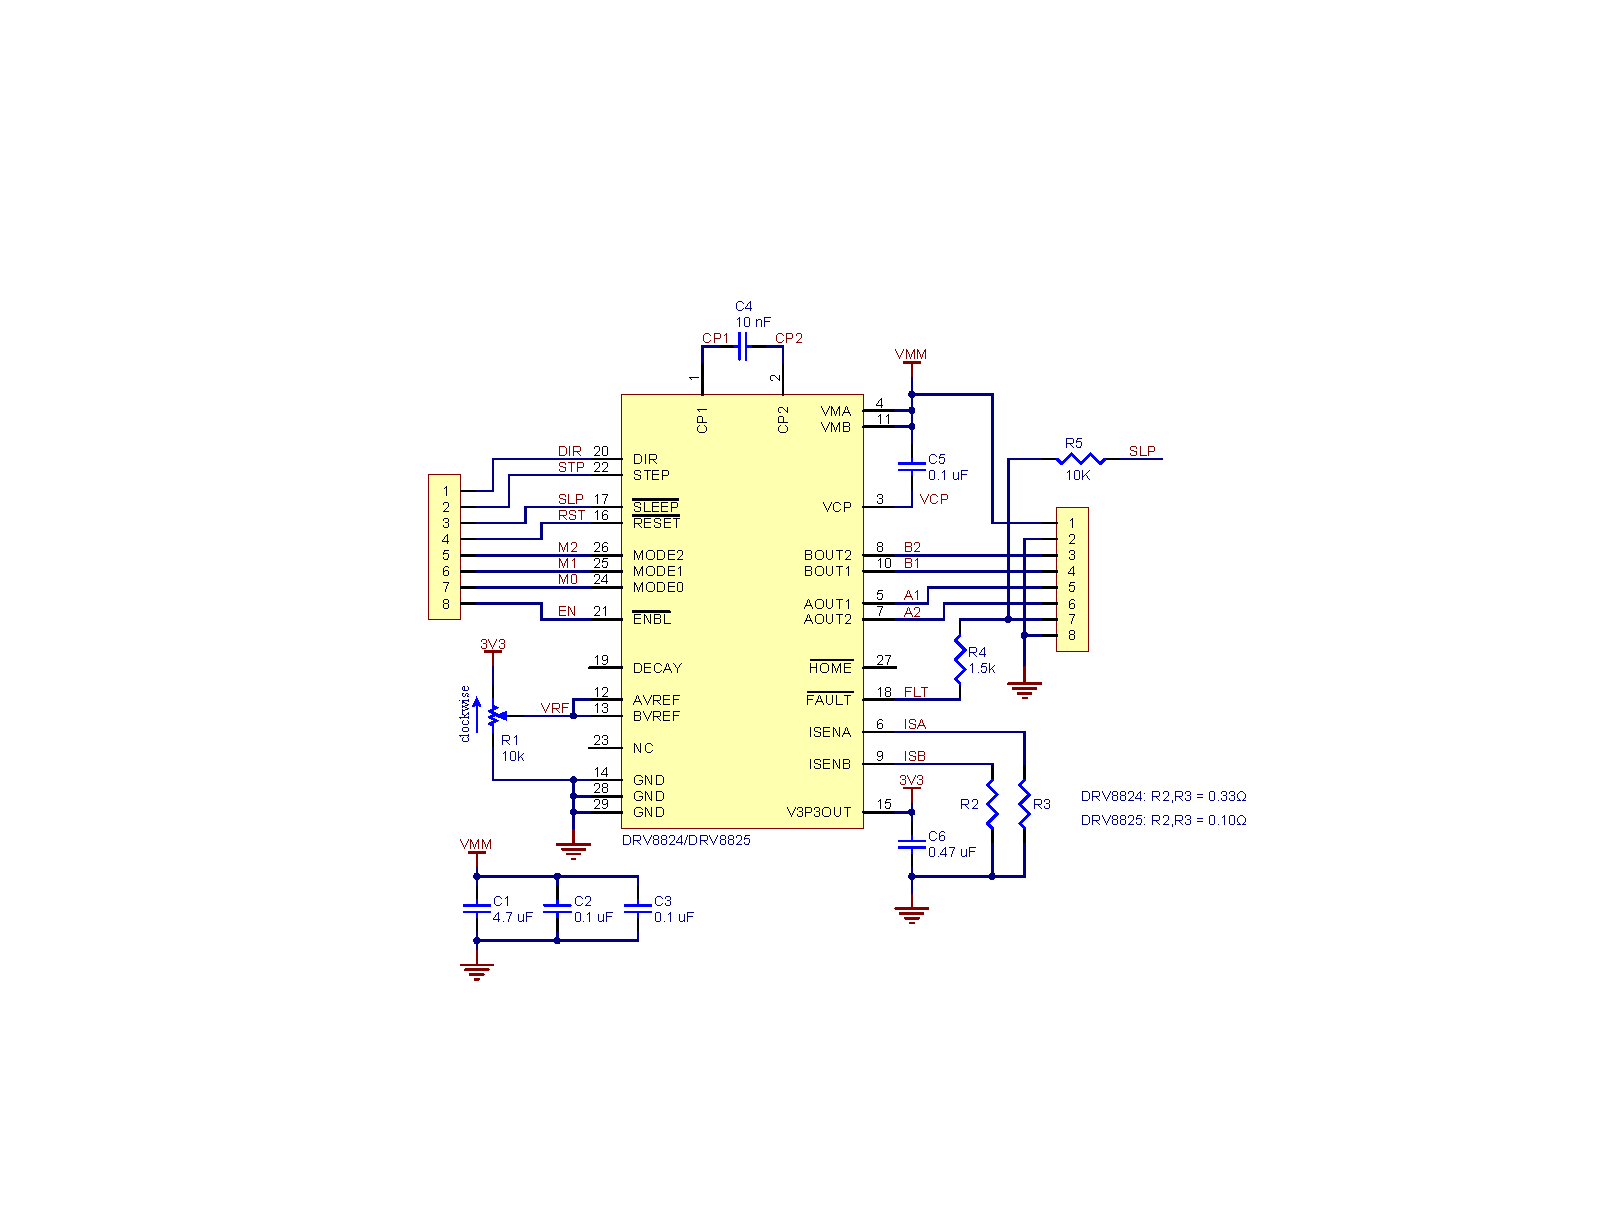
\includegraphics[width=\columnwidth]{drv8824-drv8825-stepper-motor-driver-carrier-schematic-diagram.pdf}
    \caption{DRV8825模块设计 DRV8824/DRV8825 Stepper Motor Driver Carrier}
    \label{fig:DRV8825-stepper-motor-driver-carrier-schematic-diagram}
\end{figure}

\begin{figure}[htbp]
    \centering
    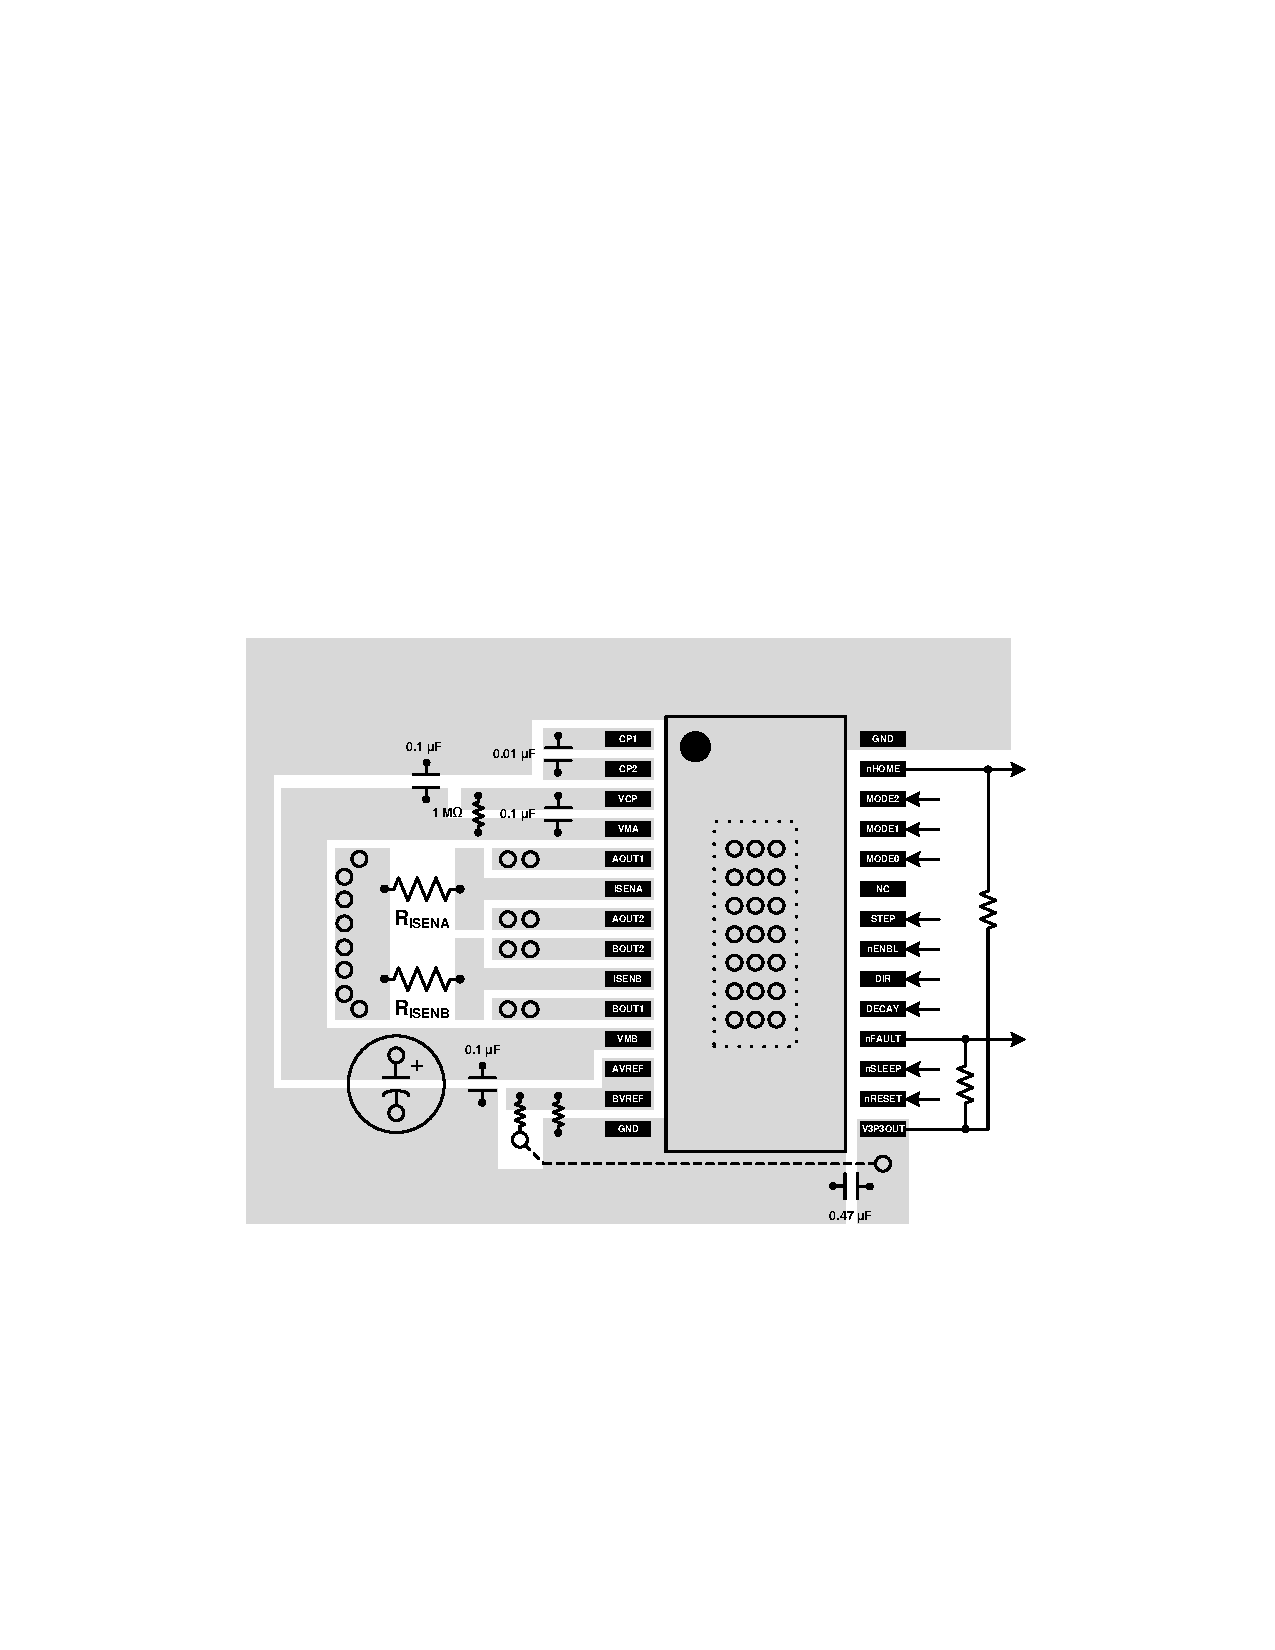
\includegraphics[width=\columnwidth]{DRV8825-Layout-Example.pdf}
    \caption{DRV8825布局参考}
    \label{fig:DRV8825-Layout-Example}
\end{figure}


\section{减速步进电机}

CHS-GM1024-10BY 2相4线直径15BY全金属齿轮减速步进电机 参数如图~\ref{fig:CHS-GM1024-10BY-Specific}所示。

\begin{figure}[htbp]
    \centering
    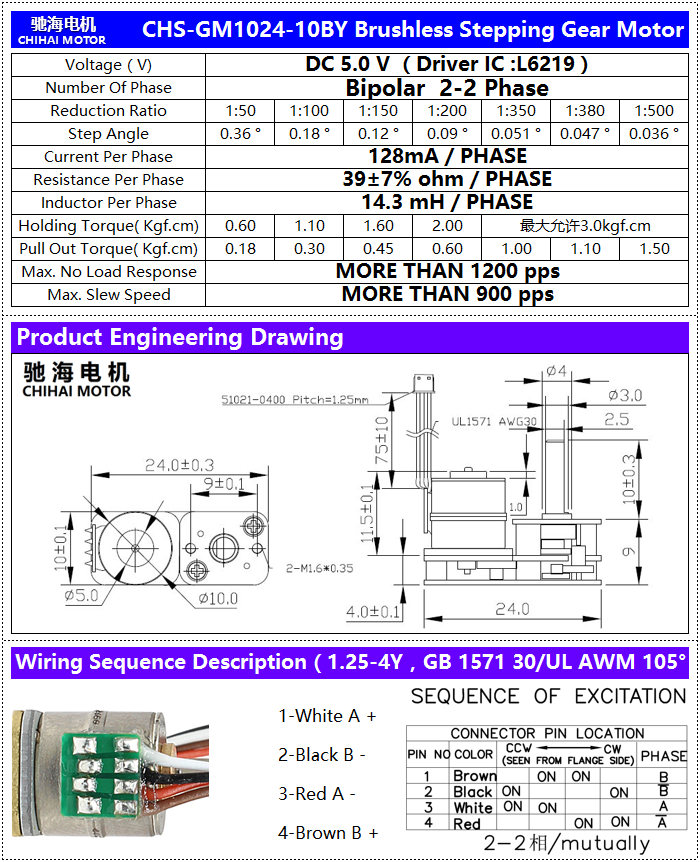
\includegraphics[width=\columnwidth]{CHS-GM1024-10BY-Specific.jpg}
    \caption{CHS-GM1024-10BY参数}
    \label{fig:CHS-GM1024-10BY-Specific}
\end{figure}

\begin{table}[htbp]
    \centering
    \begin{tabular}{ll}
    \hline
    Model                  & CHS-GM1024-10BY   \\ \hline
    Working voltage        & DC 5V             \\ \hline
    Phase                  & 2 phase 4 wire    \\ \hline
    Reduction ratio        & 1:100             \\ \hline
    Step angle             & 0.18°             \\ \hline
    Phase current          & 128mA/phase       \\ \hline
    Phase resistance       & 39±7\%ohm/phase   \\ \hline
    Phase inductance       & 14.3mH/phase      \\ \hline
    Holding torque         & 1.10kgf.cm        \\ \hline
    Pull out torque        & 0.30kgf.cm        \\ \hline
    Max starting frequency & More than 1200pps \\ \hline
    Response frequency     & More than 900pps  \\ \hline
    \end{tabular}
    \caption{CHIHAI MOTOR DC 5V Brushless Motor 2 Phase 4 Wire Stepper Motor Specification}
    \label{tab:CHS-GM1024-10BY-Specific}
\end{table}

\section{电机连接器}

采用的电机原装为Molex 51021-0400 连接器 1.25mm Pitch, PicoBlade 1.25 DIP TYPE SMT TYPE \url{https://www.chinese.molex.com/molex/products/part-detail/crimp_housings/0510210400},为了方便未来批量制作,我们使用对应的插座,如图~\ref{fig:51021-APPLICATION-SPECIFICATION}所示。

\begin{figure}[htbp]
    \centering
    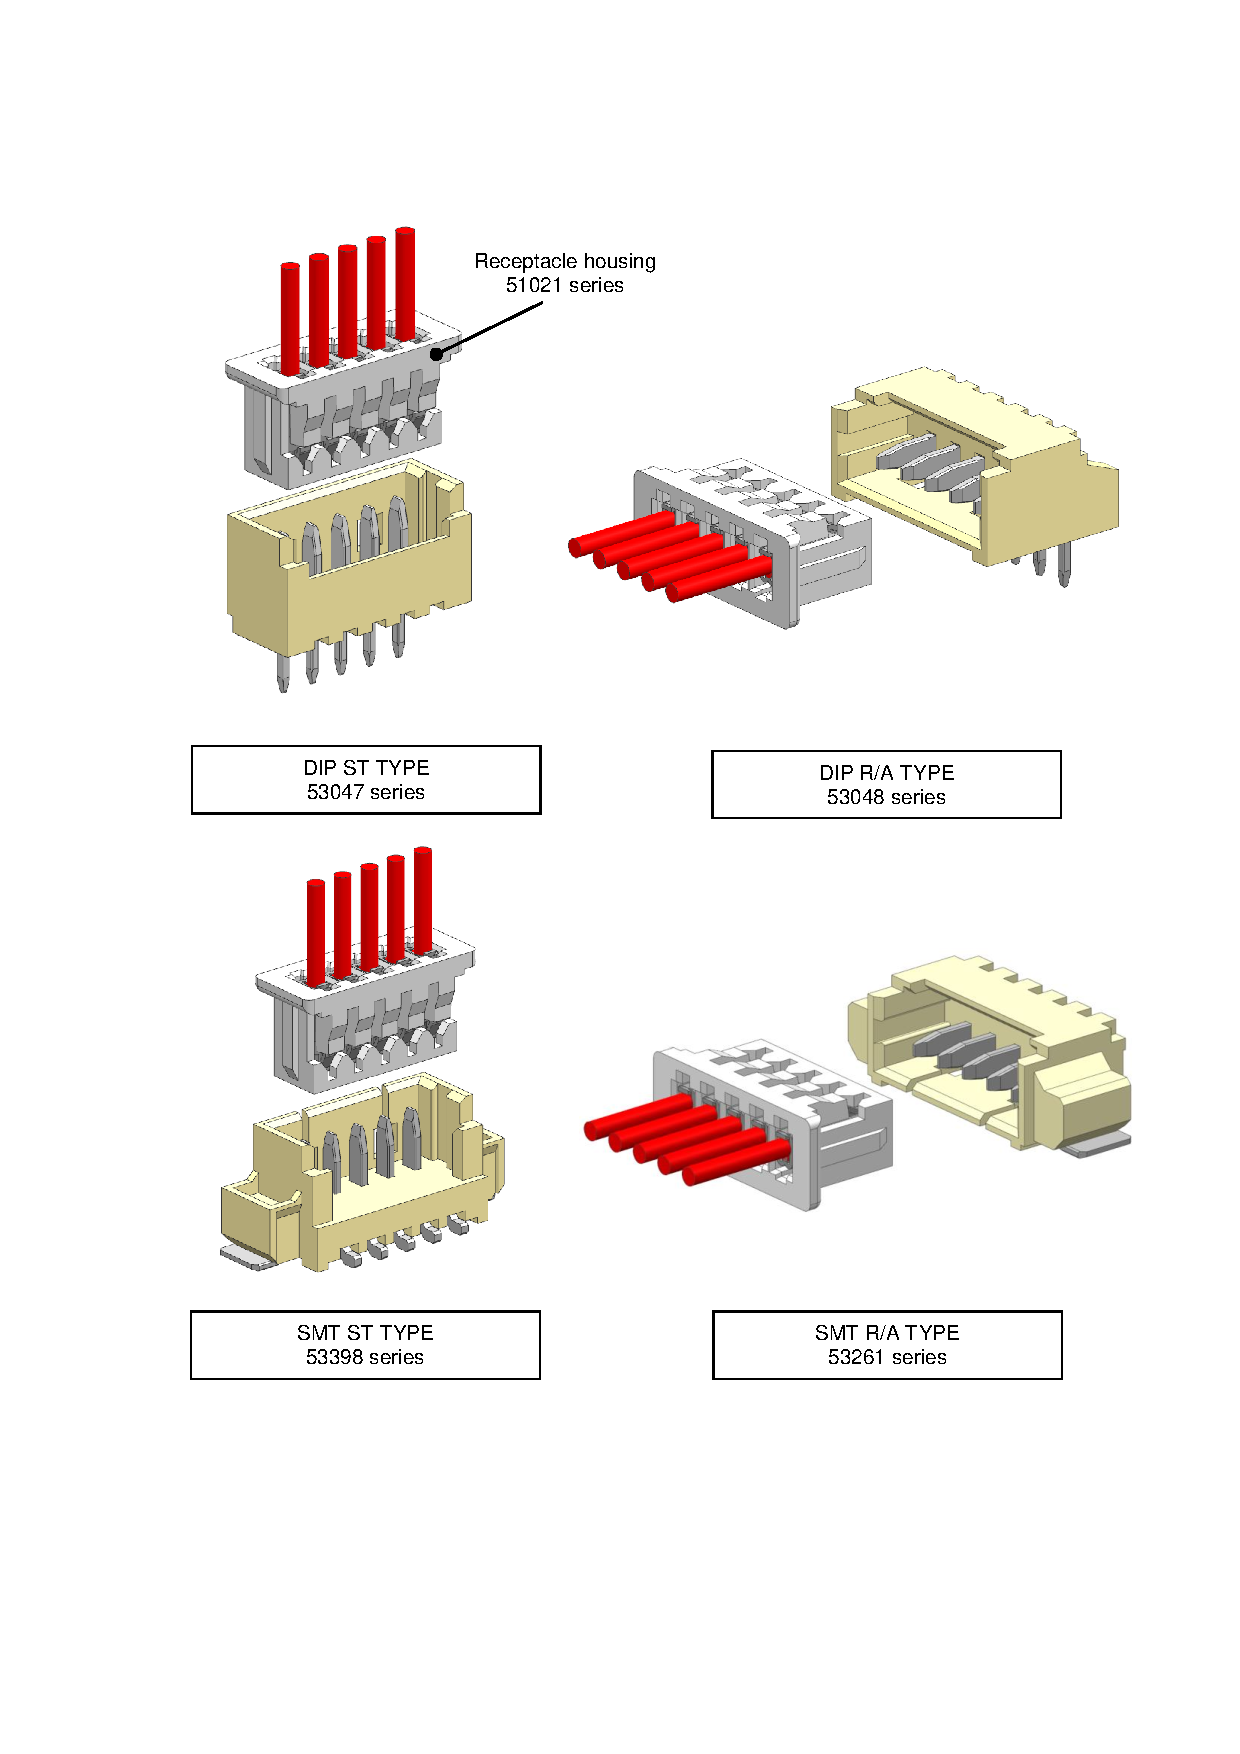
\includegraphics[width=\columnwidth]{51021-APPLICATION-SPECIFICATION.pdf}
    \caption{Molex 51021 连接}
    \label{fig:51021-APPLICATION-SPECIFICATION}
\end{figure}


\section{DRV8825 Arduino 控制程序}

本节设计源文件和历史版本详见\url{https://github.com/TingliangZhang/Misaka-Code}

pps (pulses per second)

Arduino 官方库中默认带有 Stepper Library (\url{https://www.arduino.cc/en/Reference/Stepper}),提供了unipolar or bipolar stepper motors的控制函数。

Stepper(steps, pin1, pin2, pin3, pin4) 函数定义了一个步进电机类的实例

steps: the number of steps in one revolution of your motor. If your motor gives the number of degrees per step, divide that number into 360 to get the number of steps (e.g. 360 / 3.6 gives 100 steps). (int)

问题是Stepper Library针对的是H桥或直连的2/4线简单的步进电机,并非特定的驱动芯片如DRV8825,所以需要其他库。

AccelStepper library for Arduino \url{http://www.airspayce.com/mikem/arduino/AccelStepper/} 则很好的兼容了驱动芯片并且提供加速减速等功能。

AccelStepper Class Reference 参见 \url{http://www.airspayce.com/mikem/arduino/AccelStepper/classAccelStepper.html} 。

函数 AccelStepper (uint8\_t interface=AccelStepper::FULL4WIRE, uint8\_t pin1=2, uint8\_t pin2=3, uint8\_t pin3=4, uint8\_t pin4=5, bool enable=true) 定义了一个步进电机(create a new instance of the AccelStepper class)。

其中interface设置为1,即枚举变量 enum AccelStepper::MotorInterfaceType 取AccelStepper::DRIVER (1),意为连接的是具有Step and Direction pins的步进电机驱动芯片。pin1连接到步进电机驱动Step引脚,低电平到高电平跳变为步进。pin2连接到步进电机驱动Direction引脚,高电平为正向旋转。其他变量留空默认即可。

以下操作函数需要用到使用AccelStepper实例化的名字,定义小车的三个轮子的步进电机分别为Motor1、Motor2、Motor3。

\begin{itemize}
    \item setMaxSpeed
    \item setAcceleration
    \item moveTo
    \item runToPosition
    \item runSpeed
    \item distanceToGo
    \item currentPosition
\end{itemize}


\section{单电机测试}

测试接线图如图~\ref{fig:Arduino-DRV8825}

\begin{figure}[htbp]
    \centering
    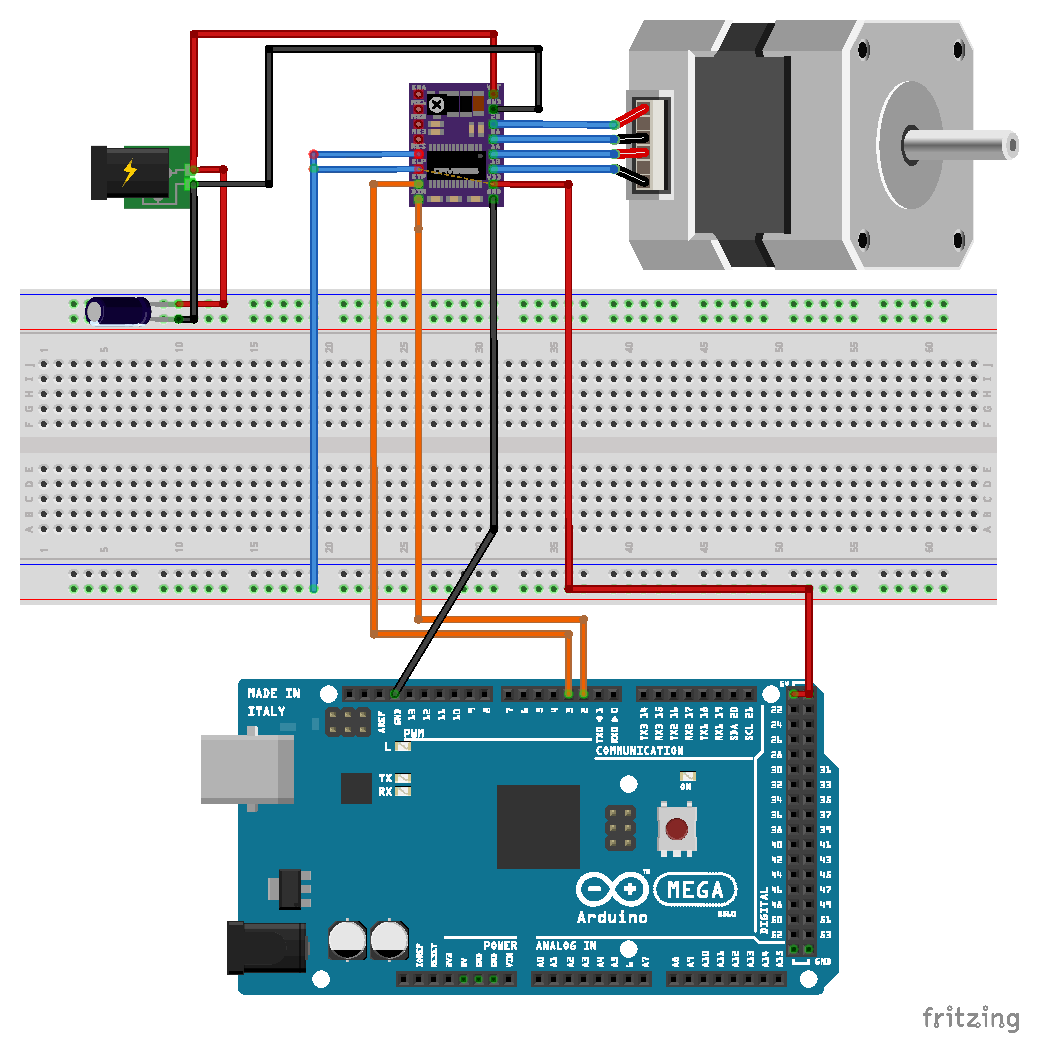
\includegraphics[width=\columnwidth]{Arduino-DRV8825-RE-SAVE.pdf}
    \caption{Arduino-DRV8825接线图}
    \label{fig:Arduino-DRV8825}
\end{figure}


% ERROR!!!!!!!
% xdvipdfmx:fatal: pdf_link_obj(): passed invalid object.
% \begin{figure}[htbp]
%     \centering
%     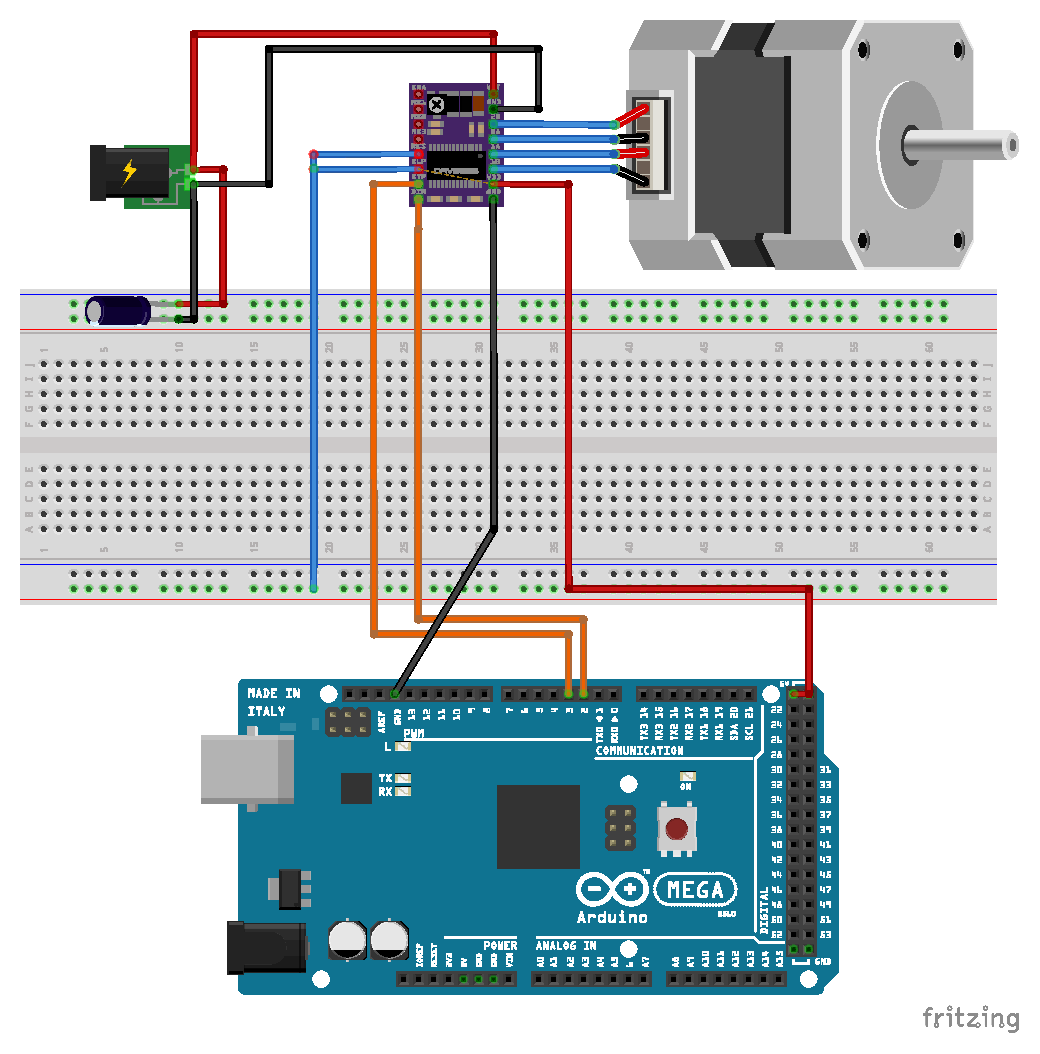
\includegraphics[width=\columnwidth]{Arduino-DRV8825.pdf}
%     \caption{Arduino-DRV8825接线图}
%     \label{fig:Arduino-DRV8825}
% \end{figure}

未接电机时使用如下代码进行加减速测试:

\inputminted[mathescape, linenos, breaklines]{C}{Code/Stepper-3/Stepper-3.ino}

得到波形如图~\ref{fig:AccelStepper-Acceleration-Waveform}、图~\ref{fig:AccelStepper-Acceleration-Waveform-with-motor}、图~\ref{fig:AccelStepper-Acceleration-Spectrogram}。

\begin{figure}[htbp]
    \centering
    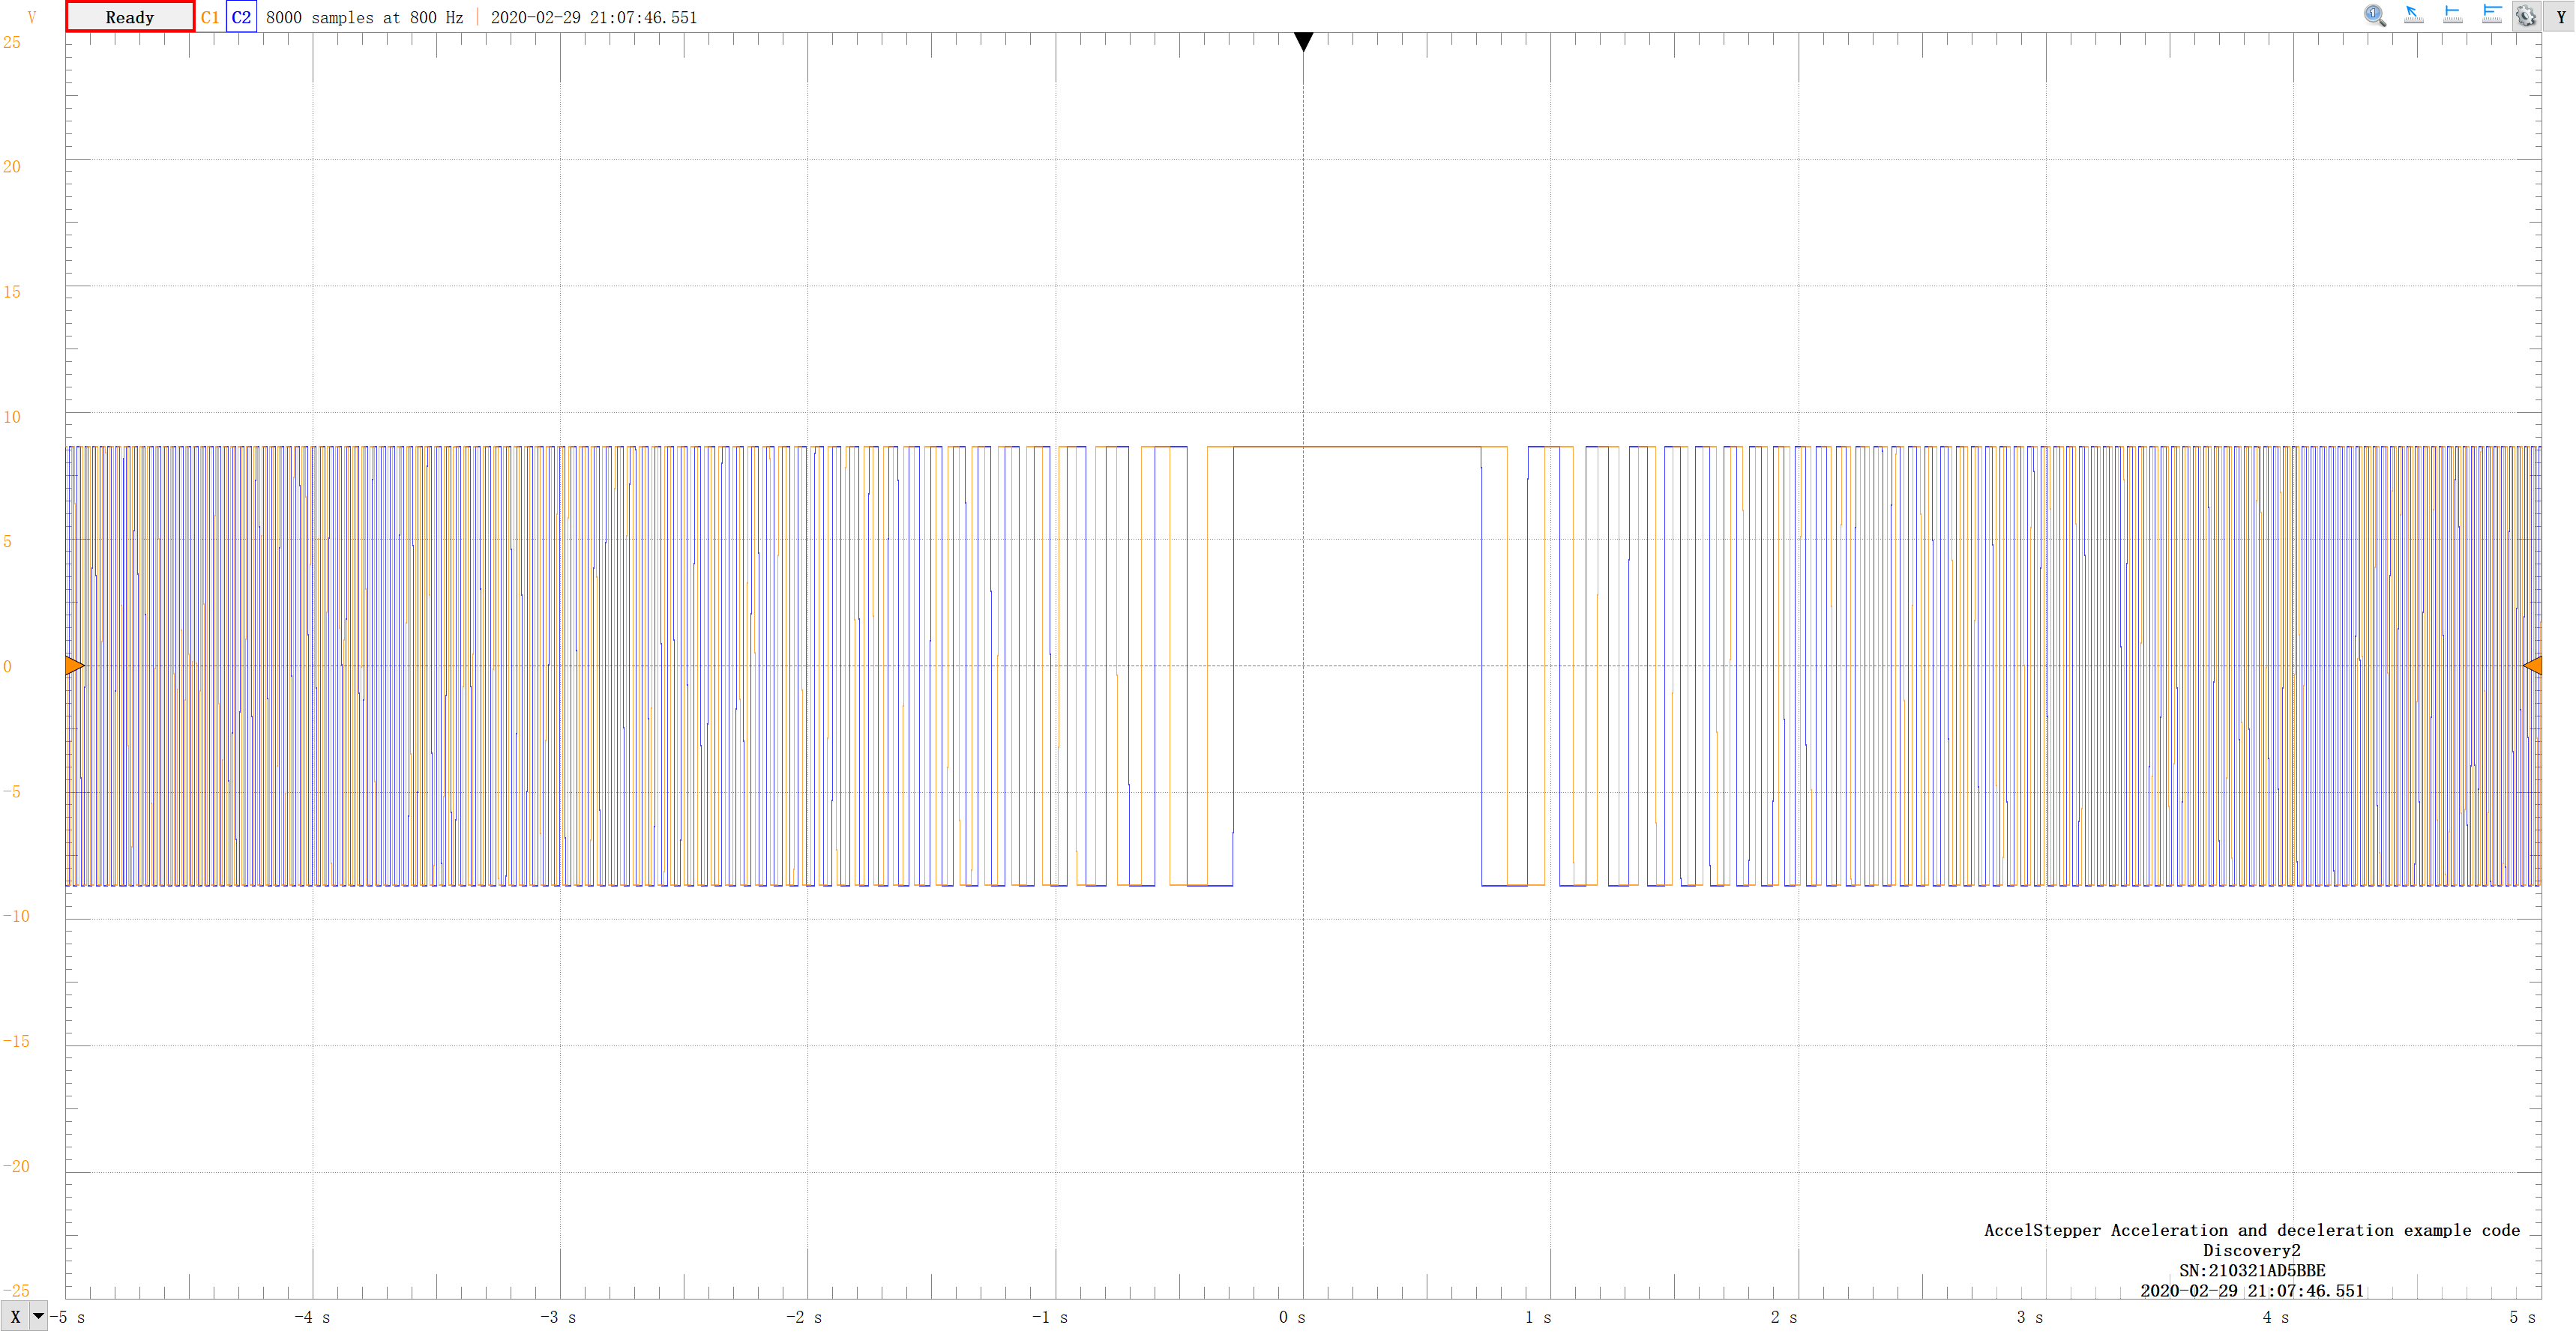
\includegraphics[width=\columnwidth]{AccelStepper-Acceleration-Waveform.png}
    \caption{AccelStepper库加速转动DRV8825未接电机输出驱动波形}
    \label{fig:AccelStepper-Acceleration-Waveform}
\end{figure}

\begin{figure}[htbp]
    \centering
    \includegraphics[width=\columnwidth]{AccelStepper-Acceleration-Spectrogram.png}
    \caption{AccelStepper库加速转动DRV8825未接电机驱动输出频谱图}
    \label{fig:AccelStepper-Acceleration-Spectrogram}
\end{figure}

\begin{figure}[htbp]
    \centering
    \includegraphics[width=\columnwidth]{AccelStepper-Acceleration-Waveform-with-motor.png}
    \caption{AccelStepper库加速转动DRV8825接电机输出驱动波形}
    \label{fig:AccelStepper-Acceleration-Waveform-with-motor}
\end{figure}

接电机时使用如下代码进行以一定加速度加速到恒定速度测试:

\inputminted[mathescape, linenos, breaklines]{C}{Code/Stepper-3/Stepper-3.ino}

得到波形如图~\ref{fig:AccelStepper-Constant-Speed-Waveform-with-motor}和图~\ref{fig:AccelStepper-Constant-Speed-Waveform-with-motor-Scaled}。

\begin{figure}[htbp]
    \centering
    \includegraphics[width=\columnwidth]{AccelStepper-Constant-Speed-Waveform-with-motor.png}
    \caption{AccelStepper库恒速转动DRV8825接电机输出驱动波形}
    \label{fig:AccelStepper-Constant-Speed-Waveform-with-motor}
\end{figure}

\begin{figure}[htbp]
    \centering
    \includegraphics[width=\columnwidth]{AccelStepper-Constant-Speed-Waveform-with-motor-Scaled.png}
    \caption{AccelStepper库恒速转动DRV8825接电机输出驱动波形(放大)}
    \label{fig:AccelStepper-Constant-Speed-Waveform-with-motor-Scaled}
\end{figure}

\section{动力系统测试}

三电机在3D打印出的测试用底盘测试,以确定扭矩是否足够带动平台。
\chapter{运动学分析和运动控制}
\label{cha:Movement}


\chapter{主板及扩展板PCB设计}
\label{cha:PCB}

主板PCB设计如图~\ref{fig:CorePCB}:

\begin{figure}[htbp]
    \centering
    \includegraphics[width=\columnwidth]{ArduinoMega2560-Core-White-Crop.pdf}
    \caption{Mega 2560主板设计}
    \label{fig:CorePCB}
\end{figure}

\section{主控ATmega2560-16AU}

主控芯片采用ARDUINO MEGA 2560 REV3\cite{arduino_mega-2560-r3}上使用的ATmega2560-16U芯片\footnote{\href{http://www.atmel.com/Images/Atmel-2549-8-bit-AVR-Microcontroller-ATmega640-1280-1281-2560-2561_datasheet.pdf}{ATmega2560 Datasheet}},并参考MEGA 2560的芯片外设和烧写器设计。引脚映射图见附录~\ref{sec:Pin2560}。

\begin{figure}[htbp]
    \centering
    \includegraphics[width=0.7\textwidth]{PinMap2560big_Rev2.png}
    \caption{Mega 2560 PIN diagram}
    \label{fig:PinMap2560}
\end{figure}

ATmega2560是高性能,低功耗基于Microchip 8位AVR RISC的微控制器(MCU),256KB ISP闪存,8KB SRAM,4KB EEPROM,86个GPIO,32个通用工作寄存器,实时计数器,六个具有比较模式的灵活定时器/计数器,PWM,4个USART,面向字节的2线串行接口,16通道10位A/D转换器以及用于片上调试的JTAG接口。该器件在16 MHz时可达到16 MIPS的吞吐量,并在4.5至5.5伏之间工作。通过在单个时钟周期内执行指令,该设备可实现接近1MIPS/MHz的吞吐量,从而平衡了功耗和处理速度。

\begin{figure}[htbp]
    \centering
    \includegraphics[]{Mega2560-ATmega2560-16AU.pdf}
    \caption{Mega 2560 MCU 原理图}
    \label{fig:Mega2560-ATmega2560-16AU}
\end{figure}

\section{供电和稳压电路}

\begin{figure}[htbp]
    \centering
    \includegraphics[]{Mega2560-Power.pdf}
    \caption{供电和稳压电路}
    \label{fig:Mega2560-Power}
\end{figure}

如图~\ref{fig:Mega2560-Power},外部锂电通过PWRIN接口输入7-15v直流,两级滤波,使用小电容100nF滤除高频干扰,大电容47uF消除低频干扰,M7为二极管,防止错误输入负电压。低压差线性稳压(LDO)降压芯片LD1117S50CTR完成电平转换,输出5V直流,在输出端也加入了一个47uF的滤波电容,滤除输出5V中的低频谐波。

高通滤波电容原本建议方案使用47uF 35V贴片型铝电解电容器,但是考虑到后续可能要堆叠电路板模块,需要尽可能的减小电路板上元件的最大高度,而6.3x5.4x5.4mm SMD 封装高度达到5.4mm。

可以用CASE-E_7343封装47uF 35V钽电容\footnote{钽电容全称是钽电解电容,也属于电解电容的一种,使用金属钽做电介质}。多数情况下,在不考虑容量和耐压时钽电解可以替换铝电解,但在耐受瞬态尖峰过压和瞬态大电流放电方面,钽电解不及铝电解,某些场合下的一些变通用法,会使电容两端施加小幅反向电压,钽电解也不可以这样。

固体钽电容器电性能优良,工作温度范围宽,而且形式多样,体积效率优异,具有其独特的特征:钽电容器的工作介质是在钽金属表面生成的一层极薄的五氧化二钽膜。此层氧化膜介质与组成电容器的一端极结合成一个整体,不能单独存在。因此单位体积内所具有的电容量特别大。即比容量非常高,因此特别适宜于小型化。但是钽电容

钽电容具有较大的ESR(串连等效电阻)值,瞬态大电流放电特性因而不佳,用于电源的主滤波是不行的,但其串连等效电感低于常见卷绕而成的铝电解,故高频滤波特性比铝电解好,适用于对付高频分量的辅助滤波。

AVCC是端口F和A/D转换器的电源电压引脚。即使不使用ADC,它也应从外部连接到VCC。如果使用ADC,则应通过低通滤波器将其连接到VCC。

LP2985-33DBVR则是另一个低压差线性稳压(LDO),它将5V降到3.3V。根据Datasheet,在布线时,旁路电容器的放置应尽可能的接近器件的VIN和系统的GND,注意使旁路电容器连接VIN引脚和系统的GND引脚形成的环路面积最小。

绿色LED串联1KOhm保护电阻,当电路接上电源时,ON LED将发光作为提示。

\begin{figure}[htbp]
    \centering
    \includegraphics[]{Mega2560-USB-POWER.pdf}
    \caption{USB供电选择电路}
    \label{fig:Mega2560-USB-POWER}
\end{figure}

如图~\ref{fig:Mega2560-USB-POWER},LM358DR2G为增益带宽积(GBP)1MHz的通用双路运放,AO3401A则为P沟道MOS(场效应管),低电平导通。

LM358DR2G的B路运放在这里作为电压比较器使用,若VIN大于6.6V,即有锂电输入,此时运放输出高电平,PMOS关断,此时板上供电由锂电提供,同时也切断了USB,防止通过锂电给USB供电的情况出现。当VIN没有输入,即没有锂电输入,如果此时USB接通,PMOS导通,USB可以直接给板子供应5V直流。

\section{MCU附属IO}

\begin{figure}[htbp]
    \centering
    \includegraphics[]{Mega2560-Core-IO.pdf}
    \caption{MCU附属IO}
    \label{fig:Mega2560-Core-IO}
\end{figure}

如图~\ref{fig:Mega2560-Core-IO},LM358DR2G的A路运放在这里作为电压跟随器,作为黄色LED的驱动,接收PB7即D13引脚的数字输入,控制黄色LED的亮灭。

2x3的端子是ICSP (In-Circuit Serial Programming) 端口,可以通过这个6Pin端口给ATmega2560 MCU烧写程序。结合AVR-ISP (in-system programmer)比如Arduino ISP\footnote{https://store.arduino.cc/usa/arduino-isp}使用。

使用Arduino ISP,可以上传脚本并在任何基于AVR的板上烧写引导程序。通过使用外部编程器上传Sketch,可以删除引导程序bootloader。Arduino ISP还可用于刻录Arduino bootloader,因此,如果不小心损坏了bootloader,则可以用它来恢复。当使用新的ATmega MCU时,也有必要刷引导程序,将希望使用的引导程序通过USB-Serial连接上传。

SCL和SDA为I2C(Inter-Integrated Circuit)集成电路总线,是一种串行通讯汇流排,使用多主从架构,只使用两条双向漏极开路(Open Drain)(串行资料(SDA)及串行时脉(SCL))并利用电阻将电位上拉。这里两个10kOhm电阻即为I2C上拉电阻。

按下轻触开关,MCU的RESET从高电平变为低电平,MCU中的程序复位,相当于重启。

CSTCE16M0V53为16MHz晶振,内置电容,作为MCU的外部时钟晶振使用。

\section{ATmega16U2}

\begin{figure}[htbp]
    \centering
    \includegraphics[]{Mega2560-ATmega16U2-MU.pdf}
    \caption{Mega2560-ATmega16U2-MU}
    \label{fig:Mega2560-ATmega16U2-MU}
\end{figure}

如图~\ref{fig:Mega2560-ATmega16U2-MU},板上的ATmega16U2芯片充当计算机的USB端口和主处理器ATmega2560-16AU的串行端口之间的桥梁。它运行称为固件的软件(之所以这样命名,是因为一旦在芯片中对其进行编程就无法更改),该软件可以通过称为DFU(设备固件更新)的特殊USB协议\footnote{https://www.arduino.cc/en/Hacking/DFUProgramming8U2}进行更新。

\begin{figure}[htbp]
    \centering
    \includegraphics[]{Mega2560-MU-IO.pdf}
    \caption{Mega2560-MU-IO}
    \label{fig:Mega2560-MU-IO}
\end{figure}

如图~\ref{fig:Mega2560-MU-IO}:

2x3的端子是ICSP (In-Circuit Serial Programming) 端口,可以通过这个6Pin端口给ATmega16U2 MCU烧写程序。

Rp1为一个排阻,上有四个相同阻值(1kOhm)的电阻,上面两个电阻作为两个黄灯的保护电阻,两个黄灯作为RX1和TX1数据传输的指示。另两个电阻则是从ATmega16U2到ATmega2560-16AU的通信线路上的电阻,通过ATmega2560-16AU的PE0和PE1给MCU烧写程序。

RESET-EN为自动复位设计,可以通过主机复位。这样通过Arduino软件烧写程序到Mega2560中软件可以自动复位,不需要再按复位按钮。在PCB上切断"RESET EN"处两个焊盘中间的线可以禁止该功能。

\section{USB接口}

通过通用串行总线(英语:U niversal S erial B us,缩写:USB)对MCU进行程序烧写和部分数据交换,同时可以给电路板供电。

USB在速度上远比并行端口(例如EPP、LPT)与串行接口(例如RS-232)等传统电脑用标准汇流排快上许多。USB 2.0(USB 2.0 HiSpeed)为480Mbps,USB 3.0(USB 3.2 Gen1)为5Gbps,USB 3.1(USB 3.2 Gen2x1)为10Gbps,而USB 3.2(USB 3.2 Gen2x2)更达20Gbps。

由于不需要过快的数据交换速度,选用USB 2.0(USB 2.0 HiSpeed)协议进行数据交换。

% https://tex.stackexchange.com/questions/316435/how-to-put-6-images-in-3-columns-2-rows/316444
% 在此环境插入png会报错,得是pdf
% https://tex.stackexchange.com/questions/17734/cannot-determine-size-of-graphic
\begin{figure}[htbp]
    \centering % <-- added
    \begin{subfigure}{0.25\textwidth}
    \includegraphics[width=\linewidth]{USB_Type-A.pdf}
    \caption{USB Type-A 公头}
    \label{fig:USB-1}
    \end{subfigure}\hfil % <-- added
    \begin{subfigure}{0.25\textwidth}
    \includegraphics[width=\linewidth]{USB_Micro-B.pdf}
    \caption{USB Micro-B 公头}
    \label{fig:USB-2}
    \end{subfigure}\hfil % <-- added
    \begin{subfigure}{0.25\textwidth}
    \includegraphics[width=\linewidth]{USB_Type-C_icon.pdf}
    \caption{USB Type-C 公头}
    \label{fig:USB-3}
    \end{subfigure}

    \medskip
    \begin{subfigure}{0.25\textwidth}
    \includegraphics[width=\linewidth]{USB_Type-A_receptacle.pdf}
    \caption{USB Type-A 母头}
    \label{fig:USB-4}
    \end{subfigure}\hfil % <-- added
    \begin{subfigure}{0.25\textwidth}
    \includegraphics[width=\linewidth]{USB_Micro-B_receptacle.pdf}
    \caption{USB Micro-B 母头}
    \label{fig:USB-5}
    \end{subfigure}\hfil % <-- added
    \begin{subfigure}{0.25\textwidth}
    \includegraphics[width=\linewidth]{USB_Type-C_receptacle.pdf}
    \caption{USB Type-C 母头}
    \label{fig:USB-6}
    \end{subfigure}
    \caption{USB 2.0 机械电子标准一览}
    \label{fig:USB-M}
\end{figure}


如表~\ref{fig:USB-M},USB的连接器分为A、B两种,分别用于主机和设备;其各自的小型化的连接器是Mini-A, Mini-B 和 Micro-A, Micro-B,另外还有Mini-AB(可支持Mini-A及Mini-B)的插口。USB 3.1版本中引入了支持正反面不区分插入的C型。

普通电脑上使用的是Type-A口,所以连接电路板时会使用Type-A转Micro USB或Type-C的USB2.0数据线。USB插槽本身还能提供5V的主动电压,及0.5A的电流。

在标准USB接口Type-A中,有四个连接器触点如表~\ref{tab:USB-4},USB信号使用分别标记为D+和D-的双绞线传输,它们各自使用半双工的差分信号并协同工作,以抵消长导线的电磁干扰。

% Please add the following required packages to your document preamble:
% \usepackage{booktabs}
\begin{table}[]
    \centering
    \begin{tabular}{@{}lll@{}}
    \toprule
    触点 & 功能(主机)             & 功能(设备)            \\ \midrule
    1  & V BUS(4.75-5.25 V) & V BUS(4.4-5.25 V) \\
    2  & D-                 & D-                \\
    3  & D+                 & D+                \\
    4  & 接地                 & 接地                \\ \bottomrule
    \end{tabular}
    \caption{标准USB Type-A连接器触点}
    \label{tab:USB-4}
\end{table}

使用Micro-USB机械电子标准的USB插座(母头),此标准常用于移动电话、平板电脑等。Micro-USB将成为移动设备数据和电源的标准接口。

Micro-USB除了第4针外,其他接口功能皆与标准USB相同如表~\ref{tab:MicroUSB}。第4针成为ID,地线在Micro-USB上连接到第5针,在Micro-USB可以悬空亦可连接到第5针。

% Please add the following required packages to your document preamble:
% \usepackage{booktabs}
\begin{table}[]
    \centering
    \begin{tabular}{@{}lll@{}}
    \toprule
    触点 & 功能                & 颜色 \\ \midrule
    1  & V BUS(4.4–5.25 V) & 红  \\
    2  & D−                & 白  \\
    3  & D+                & 绿  \\
    4  & ID                &    \\
    5  & 接地                & 黑 \\ \bottomrule
    \end{tabular}
    \caption{Micro USB连接器触点}
    \label{tab:MicroUSB}
\end{table}

也可以使用支持正反插的USB Type-C接口进行供电和烧写程序,USB Type-C接口常用于新式计算机、移动电话、平板电脑等。其通讯协议和标准见图~\ref{fig:USB-Type-C-pins}和图~\ref{fig:USB-TypeC}。

\begin{figure}[htbp]
    \centering
    \includegraphics[width=\columnwidth]{Figure-2-USB-Type-C-pins.jpg}
    \caption{USB-Type-C-pins}
    \label{fig:USB-Type-C-pins}
\end{figure}

\begin{figure}[htbp]
    \centering
    \includegraphics[width=\columnwidth]{USB-2-To-Type-C.pdf}
    \caption{USB-TypeC}
    \label{fig:USB-TypeC}
\end{figure}



\begin{figure}[htbp]
    \centering
    \includegraphics[]{Mega2560-USB.pdf}
    \caption{Mega2560-USB}
    \label{fig:Mega2560-USB}
\end{figure}

如图~\ref{fig:Mega2560-USB}:

BLM21PG300SN1D为(电感式)片式铁氧体磁珠,阻抗30Ω频率100MHz。

0603ESDA-05N为ESD抑制器/TVS二极管,箝位电压	50V,反向关断电压(典型值)	5V

USB口外壳和内部引线之间并联了ESD二极管和铁氧体磁珠,用于防USB浪涌电流,保护电路。

SMD1812P050TF为PTC自恢复保险丝,最大电压15V,保持电流500mA,最大电流100A,跳闸电流1A,为了防止USB输入电流持续过大。

USB 3.1 C TYPE DIP+SMT CONN为USB Type-C 母头,按照USB2.0协议使用,后续可添加PD或高速数据传输等功能。


\section{电机驱动}


\section{RGBLED}


\section{扩展接口}

三明治扩展。


\chapter{PCB v2.0 设计和测试}
\label{cha:PCB-v2}

本章设计源文件和历史版本详见\url{https://github.com/TingliangZhang/Misaka-PCB-v2},其中包括分层原理图、PCB设计、Gerber。

总原理图如图~\ref{fig:Circuit-1}所示。

\begin{figure}[htbp]
    \centering
    \includegraphics[width=\columnwidth]{Circuit-1.pdf}
    \caption{原理图}
    \label{fig:Circuit-1}
\end{figure}

第二版本PCB主要着眼于实际平台机械结构和PCB的配合,考虑到平台外轮廓是120mm直径圆内接正六边形,故将PCB画成100mm直径圆内接正六边形并预留三个固定孔位,对应的电机驱动及接口也对应到电机所在的位置。另外在前一个版本的PCB中存在的问题在这个版本中尽可能予以纠正。变更开发环境为开源软件Kicad。

\section{需要解决的问题}

在测试版本的PCB(PCB v1)中出现了不少经过测试发现的问题,在第二版本中尽可能予以纠正:

\begin{itemize}
    \item ATmega2560的晶振封装无法手焊,而且不在嘉立创基础库里,不方便SMT
    \item PowerSTEP01过于昂贵,而且极难手动贴片。
\end{itemize}

\section{设计环境的更改}

PCB的设计依赖电子设计自动化(英语:Electronic design automation,缩写:EDA)软件。

当初绘制PCB v1时使用的时Altium Designer 20.0.9集成开发环境,如图~\ref{fig:AltiumDesignerInterface}所示。

\begin{figure}[htbp]
    \centering
    \includegraphics[width=\columnwidth]{AltiumDesignerInterface.png}
    \caption{Altium Designer 20.0.9集成开发环境}
    \label{fig:AltiumDesignerInterface}
\end{figure}

由于AD20是商业付费EDA软件,而且之前的绘制使用了Altium Live 在线供应商封装库,可移植性和便携性不是很好,即使生成了Integrated Library,也很难找到成套的规范化封装。另外AD20的源文件不是普通编辑器可以打开的文本,这使得Git代码管理变得困难。

基于以上考量,改用KiCAD开源EDA软件进行目前及将来的电路设计,

KiCAD界面如图~\ref{fig:KiCAD-Interface}所示。

\begin{figure}[htbp]
    \centering
    \includegraphics[width=\columnwidth]{KiCAD-Interface.png}
    \caption{KiCAD开源EDA软件}
    \label{fig:KiCAD-Interface}
\end{figure}

工作流程如图~\ref{fig:kicad_flowchart}。

\begin{figure}[htbp]
    \centering
    \includegraphics[width=\columnwidth]{kicad_flowchart.png}
    \caption{KiCad Workflow}
    \label{fig:kicad_flowchart}
\end{figure}

新的原理图按照分模块绘制的原则,各模块可复用。

\section{MCU}

本部分原理图如图~\ref{fig:Circuit-1}所示。其中ICSP接口可以使用ISP编程器对第一次使用的MCU烧写固件。

参考了Mega Pro Embed CH340G / ATmega2560 board \footnote{\url{https://robotdyn.com/mega-2560-pro-embed-ch340g-atmega2560-16au.html}}的设计,如图~\ref{fig:MEGA-PRO-CH340GATmega2560}。

\begin{figure}[htbp]
    \centering
    \includegraphics[width=\columnwidth]{MEGA-PRO-CH340GATmega2560.jpg}
    \caption{Mega Pro Embed CH340G / ATmega2560}
    \label{fig:MEGA-PRO-CH340GATmega2560}
\end{figure}


\section{晶振}

由于陶瓷谐振器大多需要外加电容,且封装很难拿手焊,所以选用陶瓷振荡子。

MURATA的 CSTLS16M0X51-A0 \footnote{\url{https://www.murata.com/zh-cn/products/productdetail?partno=CSTLS16M0X51-B0}}。

村田的CSTLS系列陶瓷振荡子(CERALOCK)特征如下:

\begin{enumerate}
    % \item 无需外部负载电容器即可构建振荡电路。系列产品拥有内置电容值各不相同的各种型号,可适用于各种集成电路。
    \item 无需外部负载电容器即可构建振荡电路。
    \item 在宽温度范围内稳定。
    \item 结构小巧、重量轻并表现出优异的耐冲击性能。
    % \item 可以设计用无需调校的振荡器电路
    \item 性价比高,可用性可靠。
\end{enumerate}

\section{XBee}

XBee模块通过TX1/RX1和MCU连接,如图~\ref{fig:Circuit-1}所示。

XBee模块的底座是两排1x10 Pitch = 2mm 的母排。

\section{USB UART 异步串行数据传输芯片}

% USB转UART芯片稳定程度和价格均为FT232>CH340>PL2303。

% FT232RL-REEL价格最贵,1片要27.61,1000+批量价格也要16.24每个。FT232RL/BL的优势就FTDI一直在更新驱动发布在官网,驱动经过微软认证,兼容性最好。内部固化了USB底层协议,转出来的是虚拟串口,可以固定COM口号。电路简单,数据传输稳定性好。FT232RL自带晶振,可以转RS232/TTL(常用)及RS422,RS485 高端市场专用。

% PL2303最便宜,但波特率在115200时就有可能出现延迟。

经过测试,CH340\footnote{\url{http://www.wch.cn/products/CH340.html}}可以满足需求,且批量购买1000+只要1.47一片。

CH340C内置晶振,最为合适。

下图是统一供电方式下MCU 单片机通过TTL 串口连接CH340 芯片实现USB通讯的参考电路。该产品选择自供电方式,VCC 支持5V 或者3.3V(VCC 为3.3V 时V3 需短接到VCC),完全不使用USB 总线电源VBUS(如有需要MCU可以通过I/O 串电阻后检测其是否有效)。CH340 与MCU 使用同一电源VCC,所以CH340与MCU 之间不存在双电源通过I/O相互电流倒灌的情形。

CH340没有使用到的信号线都可以悬空。对于CH340C/N/K/E/B 芯片,无需X6 和C17 及C18。

CH340C原理图如图~\ref{fig:Circuit-10}所示。

\begin{figure}[htbp]
    \centering
    \includegraphics[width=\columnwidth]{Circuit-10.pdf}
    \caption{CH340C原理图}
    \label{fig:Circuit-10}
\end{figure}

除了常规的USB转UART电路之外,还在DTR端口引出了MCU的RESET功能,每次烧写完成后自动RESET MCU。

\section{电机驱动}

电机驱动模块原理图如图~\ref{fig:Circuit-2}所示。

\begin{figure}[htbp]
    \centering
    \includegraphics[width=\columnwidth]{Circuit-2.pdf}
    \caption{电机驱动模块原理图}
    \label{fig:Circuit-2}
\end{figure}

其中,MS1-3可以用来选择步进模式,由一个拨码开关控制。

AVREF则可以限定电流上限,这里我们先按照单电机128mA计算。之后如果涉及到替换电机,相应的更换电阻即可。

\section{供电}

供电模块原理图如图~\ref{fig:Circuit-5}所示。

\begin{figure}[htbp]
    \centering
    \includegraphics[width=\columnwidth]{Circuit-5.pdf}
    \caption{供电模块原理图}
    \label{fig:Circuit-5}
\end{figure}

使用两片AMS1117芯片将电压从12V降至5V再降至3.3V,以供逻辑电路使用。

之后考虑使用USB PD,比如使用USB PD等多快充协议芯片CH236\footnote{\url{http://www.wch.cn/products/CH236.html}}

\section{Jetson NANO接口}

Jetson NANO接口模块原理图如图~\ref{fig:Circuit-6}所示。

\begin{figure}[htbp]
    \centering
    \includegraphics[width=0.5\columnwidth]{Circuit-6.pdf}
    \caption{Jetson NANO接口模块原理图}
    \label{fig:Circuit-6}
\end{figure}

预留了一个UART串口用于Jetson NANO和MCU之间的数据交换。

\section{定位相机}

定位相机模块原理图如图~\ref{fig:Circuit-7}所示。

\begin{figure}[htbp]
    \centering
    \includegraphics[width=\columnwidth]{Circuit-7.pdf}
    \caption{定位相机模块原理图}
    \label{fig:Circuit-7}
\end{figure}

为了烧写 24LC02 EEPROM 方便,使用DIP-8 EEPROM底座方便取下和安装EEPROM。

特别注意,相机模块的2x4 1.27mm排母需要安装在PCB背面的正中央,以便对准模型中央的孔。

\section{WS2812B}

WS2812B模块原理图如图~\ref{fig:Circuit-8}所示。

\begin{figure}[htbp]
    \centering
    \includegraphics[width=\columnwidth]{Circuit-8.pdf}
    \caption{WS2812B模块原理图}
    \label{fig:Circuit-8}
\end{figure}

定义了8个串联的WS2812B和稳压电容,通过MCU的一个数字引脚控制。

\section{灯光指示}

灯光指示模块原理图如图~\ref{fig:Circuit-9}所示。

\begin{figure}[htbp]
    \centering
    \includegraphics[width=0.5\columnwidth]{Circuit-9.pdf}
    \caption{灯光指示模块原理图}
    \label{fig:Circuit-9}
\end{figure}

定义了三个0603 LED,分别指示烧写TX/RX和D13引脚的电平情况。

\section{定义板子外形轮廓}

在KiCAD PCBNEW编辑器中可以直接在 'Edge.Cuts' 层使用 'Add graphic line or polygon' 定义板子外形轮廓,空格键定义相对坐标原点。

但是只能画简单的直线和圆,而且很麻烦,所以我们使用Fusion 360 导出 DXF 文件定义外形。

如图~\ref{fig:PCB-Measure-v1}。

\begin{figure}[htbp]
    \centering
    \includegraphics[width=\columnwidth]{PCB-Measure-v1.pdf}
    \caption{PCB DXF}
    \label{fig:PCB-Measure-v1}
\end{figure}


\section{布线}

% 布线方法参考下文:

% Press W or select Custom Track Width from the context menu to type in a custom track width/via size.

% To activate the router tool press the Interactive Router button Interactive Router Button or the X key. 

% Pressing V or selecting Place Through Via from the context menu while routing a track attaches a via at the end of the trace being routed. Pressing V again disables via placement. Clicking in any spot establishes the via and continues routing (unless 'Shift' is held).

% Pressing / or selecting Switch Track Posture from the context menu toggles the direction of the initial track segment between straight or diagonal.

% The router can drag track segments, corners and vias. To drag an item, click on it with Ctrl key pressed, hover the mouse and press G or select Drag Track/Via from the context menu.

% 布线之后的PCB详见附录~\ref{sec:PCB}。

布线之后的PCB正面如图~\ref{fig:CircuitPCB-F},背面如图~\ref{fig:CircuitPCB-B}。

\begin{figure}[htbp]
    \centering
    \includegraphics[width=\columnwidth]{CircuitPCB-F.pdf}
    \caption{PCB正面}
    \label{fig:CircuitPCB-F}
\end{figure}

\begin{figure}[htbp]
    \centering
    \includegraphics[width=\columnwidth]{CircuitPCB-B.pdf}
    \caption{PCB背面}
    \label{fig:CircuitPCB-B}
\end{figure}

\section{三维渲染图}

使用光线追踪技术对PCB模型进行渲染得到正反面的渲染图如图~\ref{fig:Circuit-Render}、~\ref{fig:Circuit-Render-2}、~\ref{fig:Circuit-Render-3}。

\begin{figure}[htbp]
    \centering
    \includegraphics[width=\columnwidth]{Circuit.png}
    \caption{正面渲染图}
    \label{fig:Circuit-Render}
\end{figure}

\begin{figure}[htbp]
    \centering
    \includegraphics[width=\columnwidth]{Circuit-2.png}
    \caption{反面渲染图}
    \label{fig:Circuit-Render-2}
\end{figure}

\begin{figure}[htbp]
    \centering
    \includegraphics[width=\columnwidth]{Circuit-3.png}
    \caption{侧视渲染图}
    \label{fig:Circuit-Render-3}
\end{figure}

\section{导出Gerber交付打样}

在File-Plot-Gerber中选中需要的层,压缩上传。

\section{焊接}

使用InteractiveHtmlBom\footnote{\url{https://github.com/openscopeproject/InteractiveHtmlBom}}(Interactive HTML BOM plugin for KiCad)工具导出了HTML BOM方便焊接时对照BOM,如图~\ref{fig:InteractiveHtmlBom}。

\begin{figure}[htbp]
    \centering
    \includegraphics[width=\columnwidth]{InteractiveHtmlBom.png}
    \caption{InteractiveHtmlBom}
    \label{fig:InteractiveHtmlBom}
\end{figure}

由于AT Mega的100A, 100-lead, 14 x 14 mm Body Size, 1.0 mm Body Thickness, 0.5 mm Lead Pitch, Thin Profile Plastic Quad Flat Package (TQFP)封装较难手焊,于是定制了相应的激光钢网,涂锡膏(solder paste)之后摆上元件,并使用相应的恒温锡炉加热融化锡膏,这里使用的是138度熔点的千住锡浆,锡炉温度设定在180摄氏度。如图~\ref{fig:ApplySolderPaste}。

\begin{figure}[htbp]
    \centering
    \includegraphics[width=\columnwidth]{PCBv2ApplySolderPaste.jpg}
    \caption{激光钢网涂锡膏}
    \label{fig:ApplySolderPaste}
\end{figure}

\begin{figure}[htbp]
    \centering
    \includegraphics[width=\columnwidth]{SolderOven.jpg}
    \caption{恒温锡炉(无铅预热平台)}
    \label{fig:SolderOven}
\end{figure}


正面焊完效果如图~\ref{fig:PCBv2Soldring}。

\begin{figure}[htbp]
    \centering
    \includegraphics[width=\columnwidth]{PCBv2Soldring.jpg}
    \caption{正面焊完效果}
    \label{fig:PCBv2Soldring}
\end{figure}

使用Arduino as ISP烧写Blink和Floar LED String Test程序,测试部分功能正常。如图~\ref{fig:PCBv2ISP}和图~\ref{fig:PCBv2Test}。

\begin{figure}[htbp]
    \centering
    \includegraphics[width=\columnwidth]{PCBv2ISP.jpg}
    \caption{使用Arduino as ISP烧写}
    \label{fig:PCBv2ISP}
\end{figure}

\begin{figure}[htbp]
    \centering
    \includegraphics[width=\columnwidth]{PCBv2Test.jpg}
    \caption{Floar LED String Test程序运行效果}
    \label{fig:PCBv2Test}
\end{figure}

\section{Debug}

第一次通过USB上电就出现一个严重的问题,C12炸飞,火星四溅。烧毁的PCB如图~\ref{fig:BrokenPCB}。经过排查,是5V net经过C12下方的走线宽度过小,导致大功率经过时发热过大,把整条线路熔断,看到的火花并非电容爆炸时产生的,而是基板中的顶层铜层发热积累,破坏基板和阻焊之后过热的铜片产生的火花。如图~\ref{fig:BrokenPCB},当仅使用5V供电时,几乎所有元件的功率都叠加在C12下面的走线上,当初画的板子时不合理的。测试阶段暂时外接一个5V作为替代,等待新板子交货。

\begin{figure}[htbp]
    \centering
    \includegraphics[width=\columnwidth]{PCBv2BrokenPCB.jpg}
    \caption{烧毁的PCB}
    \label{fig:BrokenPCB}
\end{figure}

\begin{figure}[htbp]
    \centering
    \includegraphics[width=\columnwidth]{BrokenPCB-5V.png}
    \caption{5V net 存在的串联瓶颈问题}
    \label{fig:BrokenPCB-Illumination}
\end{figure}

以及焊接的时候,用除去多余焊锡的烙铁头解决AT Mega引脚相连问题时,400度加热时间过长,导致芯片损坏,使用ISP烧写程序时时断时续。

重新画了PCB,4月3日终于打样完成。

4月5日焊接完成了新板子的电机驱动系统,但是上午测试了一组,电机一直没有转,没找到原因,由于一共三组电机的驱动,下午把三组驱动都焊完了,发现只有三号电机驱动是能用的,电机在转,其他两个都没转,不知道为什么,好在有能用的说明原理上没有问题,有可能是我焊的时候哪里出错了,得仔细找找。

首先排查输入,D6输出的方波脉冲如图~\ref{fig:DRV8825Debug1}。

\begin{figure}[htbp]
    \centering
    \includegraphics[width=\columnwidth]{DRV8825Debug1.png}
    \caption{D6输出的方波脉冲}
    \label{fig:DRV8825Debug1}
\end{figure}

用AD2排查发现借上12V电源后,发现3号DRV8825的12/13脚(AVREF/BVREF)电压为3.3V,但是1号为1.23V,2号为0.01V,可能IFS(Target Full-Scale Current)不足以驱动此步进电机。但实际上输出端根本没有方波信号输出,所以可能另有原因。而且3号电机发热严重,3.3V对应的IFS可能不合适。

按照我的设计1.23V是正常的,非常意外出现了3.3V和0V,现在拆掉R3和R9,让1号和2号的DRV8825的12/13脚(AVREF/BVREF)电压为3.3V。

2号空载时输出了PWM波,但是带不动电机,仔细排查发现13旁边的14号引脚(GND)和13连起来了,如图~\ref{fig:DRV8825Debug2},使得VREF一直处于低电平。使用蘸松香的350度刀头烙铁轻触连接的小块焊锡后正常。

\begin{figure}[htbp]
    \centering
    \includegraphics[width=0.8\columnwidth]{DRV8825Debug2.jpg}
    \caption{左上角的第1个和第2个角连起来了}
    \label{fig:DRV8825Debug2}
\end{figure}

1号空载时就没有输出PWM波,经排查,其27脚(nHOME)没有输出类似2/3号输出的方波,如图~\ref{fig:DRV8825Debug-25},查阅Datasheet得知,Home position : Logic low when at home state of step table,;类型为OD = open-drain output。R7为OD门的上拉电阻。

\begin{figure}[htbp]
    \centering
    \includegraphics[width=\columnwidth]{DRV8825Debug3.png}
    \caption{2/3号27脚(nHOME)输出的方波}
    \label{fig:DRV8825Debug-25}
\end{figure}

排查了所有输入引脚和滤波电容,没有发现问题,应该时芯片损坏了。使用左右横跳法替换了芯片,由于芯片下有Heatsink,新放上去的芯片很容易翘起来。新的芯片的3.3V引脚没有和PCB连接,翘起来了,小心的堆了一点焊锡连接起来,如图~\ref{fig:DRV8825Debug4}。

\begin{figure}[htbp]
    \centering
    \includegraphics[width=0.8\columnwidth]{DRV8825Debug4.jpg}
    \caption{左下角的3.3V引脚没有和PCB连接}
    \label{fig:DRV8825Debug4}
\end{figure}

现在三个电机驱动空载输出都是正确的了,但是接上三个电机后1/3号总有一个堵转,拔下来一个就好了。怀疑是12V供电线路容量不足以两个电机同时转动。

值得注意的是,现在1/2号电机驱动的VREF都是1.23V是正常的,但3号还是3.3V。尝试修一下3,可能是30kOhm断路或者50kOhm短路导致的,替换两个电阻。

通过功率表测试我们知道,系统总功率随连接电机数变化如表~\ref{tab:DRV8825Debug}所示。可以看出,三个电机时,有一个电机堵转,总功率变小,说明是供电的问题。

\begin{table}
    \centering
    \begin{tabular}{ll} 
    \toprule
    连接电机数 & 系统总功率/W  \\
    \hline
    0     & 0.6      \\
    1     & 3.6      \\
    2     & 4.8      \\
    3     & 4.2      \\
    \bottomrule
    \end{tabular}
    \caption{系统总功率随连接电机数变化}
    \label{tab:DRV8825Debug}
\end{table}

果然,供电从15W USB可调升降压电源充电模块DP2F换成2S锂电之后就一切正常了!如图~\ref{fig:DRV8825Debug5}。

\begin{figure}[htbp]
    \centering
    \includegraphics[width=0.8\columnwidth]{DRV8825Debug5.jpg}
    \caption{三个电机都转起来了}
    \label{fig:DRV8825Debug5}
\end{figure}
\chapter{PCB 3.0 改进设计和测试}
\label{cha:PCB-v3}

\section{待改进问题}

三路驱动丝印编号

电池插头+-反向,以丝印标注

芯片周围留出clearance,方便拖焊。摆放可以考虑45度角摆放,方便密集的布线。

最好改成单面有贴片元件的形式,方便SMT或者制作钢网涂锡膏。

选用没有ThermalVias的芯片封装,否则容易焊锡粘到了ThermalVias上引起不平整。(但是没有不含ThermalPad的封装)

留出STEP和DIR测试/备用引脚,以便板上有一两片DRV8825无法正常使用可以外接模块。

12V和5V供电太细了,要注意供电可靠性。

扩大PCB面积,从100mm到120mm直径圆内接正六边形。

Reset按钮封装不对。Reset电路中R22/D1,RESET BUTTON/C13不是必须的,可以画,可以不焊。

!!!发现CH340C的TX接到了Mega的TX上,RX接到了Mega的RX上,所以烧录Arduino时出现错误:

\begin{tcolorbox}
    avrdude: stk500v2\_ReceiveMessage(): timeout \\
    avrdude: stk500v2\_getsync(): timeout communicating with programmer
\end{tcolorbox}


\section{外形}

小车外轮廓为120mm圆内接正六边形,为了尽可能放到单面上,设计成120mm圆内接正六边形,加上40mm半径处3mm直径的M3螺丝定位孔,注意孔位置在边上而不是角上。注意Fusion360导出草图的操作是直接右键草图另存为DXF!

\section{原理图更改}

在这个版本,删去了一些演示中暂时用不到的模块:

\begin{itemize}
    \item RGB-LED阵列
    \item 下视相机模块
    \item 控制步进的拨码开关
    \item Reset按钮和电容/CD1206二极管
\end{itemize}

同时将XT30的正负极反向,修正了封装和实际不对应的问题。

TX0和RX0倒序,纠正了错误。

原理图如图~\ref{fig:MisakaPCBv3-sch}。

\begin{figure}[htbp]
    \centering
    \includegraphics[width=\columnwidth]{MisakaPCBv3-1.pdf}
    \caption{PCBv3原理图}
    \label{fig:MisakaPCBv3-sch}
\end{figure}

\section{PCB绘制}

将MCU倾斜45度,方便布线。

加粗12V和5V干线至1mm宽。

三个电机驱动模块统一布局布线,使其具有相似性,并变得整齐。

考虑到走线问题,同一功能的信号线组并在一起。

布线之后的PCB详见附录~\ref{sec:PCB}。

布线之后的PCB(未显示铺铜)如图~\ref{fig:MisakaPCBv3-1}、~\ref{fig:MisakaPCBv3}。

\begin{figure}[htbp]
    \centering
    \includegraphics[width=\columnwidth]{MisakaPCBv3-2.pdf}
    \caption{PCBv3布线}
    \label{fig:MisakaPCBv3}
\end{figure}

\begin{figure}[htbp]
    \centering
    \includegraphics[width=\columnwidth]{MisakaPCBv3-1.png}
    \caption{PCBv3布线之后的PCB}
    \label{fig:MisakaPCBv3-1}
\end{figure}

\section{三维渲染图}

使用光线追踪技术对PCB模型进行渲染得到正面的渲染图如图~\ref{fig:MisakaPCBv3-2}、~\ref{fig:MisakaPCBv3-3}。

\begin{figure}[htbp]
    \centering
    \includegraphics[width=\columnwidth]{MisakaPCBv3-2.png}
    \caption{正面渲染图}
    \label{fig:MisakaPCBv3-2}
\end{figure}

\begin{figure}[htbp]
    \centering
    \includegraphics[width=\columnwidth]{MisakaPCBv3-3.png}
    \caption{光追渲染图}
    \label{fig:MisakaPCBv3-3}
\end{figure}

\section{其他问题}

应当加一个ON LED作为电源指示灯。

\chapter{开发环境的配置}
\label{cha:Environment}

在这一章,着重阐述Windows 10环境下开发环境的配置方法。

\section{Mega 2560开发环境}

本节主要叙述了如何烧写Bootloader:需要两块板,Programmer和Target,首先按对应的引脚一一对应连接MISO/MOSI/SCK/Reset/GND/5V,之后给Programmer上传Arduino ISP Skectch,之后选择编程器为Arduino as ISP,烧写引导程序,如果之后要使用ICSP烧Target的程序的话,就点 项目 > 使用编程器上传即可。参考\url{https://www.arduino.cc/en/Hacking/HomePage}。

\subsection{初次使用烧写固件}

在AVR单片机的每次复位时都执行了一段特殊的代码,并使用特定的协议和速度从串行/ USB端口上载了Sketch。如果未检测到连接,则执行将传递到Sketch的代码。

这小段代码(通常为512字节)被称为“Bootloader”,如图~\ref{fig:MemoryMap},它位于微控制器的内存区域中地址空间的末尾,被设计为用于引导,不能重新编程为常规Sketch。

\begin{figure}[htbp]
    \centering
    \includegraphics[width=0.5\columnwidth]{MemoryMap.jpg}
    \caption{ATmega328P 内存映射}
    \label{fig:MemoryMap}
\end{figure}

一般来说,微控制器通过编程器被烧写程序(programmer),除非微控制器中有一个固件(firmware),该固件允许无需外部编程器而安装新固件。这种固件称为引导加载程序(bootloader)。新出厂的微控制器内部不含Bootloader,必须要先烧录引导程序

\begin{figure}[htbp]
    \centering
    \includegraphics[width=0.5\columnwidth]{Pocket-AVR-Programmer.jpg}
    \caption{Pocket AVR Programmer}
    \label{fig:Pocket-AVR-Programmer}
\end{figure}

烧写Bootloader\footnote{\url{https://www.arduino.cc/en/Hacking/Bootloader}}需要先购买AVR-ISP (in-system programmer,如图~\ref{fig:Pocket-AVR-Programmer}), USBtinyISP 或者自己做一个ParallelProgrammer(并行编程器),这些编程器需要连接到ICSP引脚(如图~\ref{fig:Isp_headers}),同时板子需要通电(USB或者电池都可以)。

\begin{figure}[htbp]
    \centering
    \includegraphics[width=0.5\columnwidth]{Isp_headers.pdf}
    \caption{6- and 10-pin ISP header}
    \label{fig:Isp_headers}
\end{figure}

在Arduino IDE中,确保 Tools > Board 选项是对的(注意要选成目标板Target的型号,比如在本项目中目标板就是Arduino Mega1280 or Mega2560),之后开始 Tools > Burn Bootloader 等待约15秒即可。

也可以使用编程器对应的软件比如AVRISP MkII的AVRStudio进行烧写操作,参考\url{https://www.arduino.cc/en/Hacking/MiniBootloader}。

另外,如果不购买专用的ISP,可以通过一块Arduino Mega 2560 开发板给本项目的电路板烧写程序\footnote{参考\url{https://www.arduino.cc/en/Hacking/Upgrading16U2Due}}。事实上,本项目就是这样给每块芯片烧写引导的。

做法如下:

在Arduino IDE里面打开示例文件 ArduinoISP并烧写到用作烧写器的Arduino上。

在 GND 和 RESET之间连接一个10uF的电容,并将Arduino Uno (or Mega)如表~\ref{tab:ICSP}所示的引脚连接到要烧写芯片的对应ICSP引脚上,如图~\ref{fig:Arduino-Mega-Mega-Sketch}。

% Please add the following required packages to your document preamble:
% \usepackage{booktabs}
\begin{table}[htbp]
    \centering
    \begin{tabular}{@{}llll@{}}
    \toprule
          & Uno & Mega & 16U2 ICSP \\ \midrule
    SCK   & 13  & 52   & 3         \\
    MISO  & 12  & 50   & 1         \\
    MOSI  & 11  & 51   & 4         \\
    Reset & 10  & 10   & 5         \\
    GND   & GND & GND  & 6         \\
    +5V   & 5V  & 5V   & 2         \\ \bottomrule
    \end{tabular}
    \caption{ICSP}
    \label{tab:ICSP}
\end{table}

\begin{figure}[htbp]
    \centering
    \includegraphics[width=\columnwidth]{Arduino-Mega-Mega-Sketch.pdf}
    \caption{Arduino-Mega-Mega-Sketch}
    \label{fig:Arduino-Mega-Mega-Sketch}
\end{figure}

最后使用avrdude命令进行固件烧写,avrdude 可以在 /path to arduino/arduino.1.8.x/hardware/tools 路径找到。

要烧写进16U2的固件是 .hex 扩展名的二进制文件,首先CMD/Terminal路径设置到avrdude所在的文件夹里,之后运行如下命令:

Windows:

\begin{tcolorbox}
    arduino-1.5.2/hardware/tool> avrdude.exe -C avrdude.conf -c arduino -P /dev/ttyACM0 -b 19200 -p m16u2 -vvv -U flash:w:/home/USER/newFirmware/16u2.hex:i
\end{tcolorbox}

Linux and Mac:

\begin{tcolorbox}
    /home/USER/arduino-1.5.2/hardware/tools\$ ./avrdude -C avrdude.conf -c arduino -P /dev/ttyACM0 -b 19200 -p m16u2 -vvv -U flash:w:/home/USER/newFirmware/16u2.hex:i
\end{tcolorbox}

avrdude参数解释见表~\ref{tab:avrdude}

\begin{table}[htbp]
    \centering
    \begin{tabular}{ll}
    -C avrdude.conf                              & load the configuration file for using the Arduino Uno as programmer       \\
    -c arduino                                   & specify the programmer you want to use                                    \\
    -P /dev/ttyACM0                              & the usb port where the programmer is attached                             \\
    -b 19200                                     & the baudrate                                                              \\
    -p m16u2                                     & the target device you want to program                                     \\
    -vvv                                         & enable the verbose output                                                 \\
    -U flash:w:/home/USER/newFirmware/16u2.hex:i & specify that you want to write (w) the  .hex file inside the flash memory
    \end{tabular}
    \caption{Avrdude parameter explanations}
    \label{tab:avrdude}
\end{table}

只要找到对应的ICSP引脚,烧写ATMega2560和ATmega16U2的操作基本一致。如图~\ref{fig:Arduino-Mega-UNO-Sketch}。

更加具体的解释见\url{https://www.arduino.cc/en/Tutorial/ArduinoISP}

\begin{figure}[htbp]
    \centering
    \includegraphics[width=\columnwidth]{Arduino-Mega-UNO-Sketch.pdf}
    \caption{Arduino-Mega-UNO-Sketch}
    \label{fig:Arduino-Mega-UNO-Sketch}
\end{figure}

\subsection{Arduino IDE}

本项目使用的ATmega2560-16AU和ATmega16U2-MU芯片组是Arduino IDE支持的,对应ARDUINO MEGA 2560 REV3开发板,因此,本开发环境将基于Arduino IDE(\url{https://www.arduino.cc/en/Main/Software})进行搭建。

\begin{figure}[htbp]
    \centering
    \includegraphics[width=\columnwidth]{Arduino-Fritzing.pdf}
    \caption{Arduino Mega}
    \label{fig:Arduino-Fritzing}
\end{figure}

Arduino集成开发环境(Arduino IDE)包含了一个用于写代码的文本编辑器、一个消息区、一个文本控制台以及一个带有常用功能按钮和文本菜单的工具栏。连接Arduino之后,软件能给所连接的控制板上传程序,还能与控制板相互通信。

使用Arduino软件(IDE)编写的代码被称为项目(sketches),这些项目写在文本编辑器中,以.ino的文件形式保存

IDE UI中上传按钮的作用是编译代码并且上传到选定的控制板中,注意:如果你使用的是专门的编程器,你需要在点击按钮时按住电脑的“shift”键,显示的文字会变成“使用编程器上传”。

在上传之前,需要在 Tools - Board 和 Tools - Port 中选定开发板类型和端口,在本项目中,选择Arduino/Genuino Mega 2560 (Arduino/Genuino Mega 2560
An ATmega2560 running at 16 MHz with auto-reset, 16 Analog In, 54 Digital I/O and 15 PWM.)开发板。

端口在Windows系统中,串口显示为 COM1 或 COM2,USB则显示为COM3及以上,选择对应的端口即可。



\section{ESP 32开发环境配置}

本节阐述搭建 ESP32 硬件开发的软件环境,软件编译和烧写流程\footnote{\url{https://docs.espressif.com/projects/esp-idf/zh_CN/v4.0-rc/get-started/}}如图~\ref{fig:ESP-Need}。

\begin{figure}[htbp]
    \centering
    \includegraphics[width=0.6\columnwidth]{ESP-Need.png}
    \caption{ESP32 应用程序开发}
    \label{fig:ESP-Need}
\end{figure}

\subsection{Windows平台ESP-IDF工具链的标准设置}

ESP-IDF 需要安装一些必备工具,才能围绕 ESP32 构建固件,包括 Python、Git、交叉编译器、menuconfig 工具、CMake和 Ninja 编译工具等。

要安装 ESP-IDF 必备工具,最简易的方式是下载 ESP-IDF 工具安装器\footnote{\url{https://dl.espressif.com/dl/esp-idf-tools-setup-2.2.exe}}。

安装器可安装所需的交叉编译器、OpenOCD、cmake 和 Ninja 编译工具,以及一款 mconf-idf 配置工具。此外,本安装器还可在有需要时下载、运行 Python 3.7 和 Git For Windows 的安装器,如图~\ref{fig:IDF-Installer}。

\begin{figure}[htbp]
    \centering
    \includegraphics[width=0.7\columnwidth]{IDF-Installer.png}
    \caption{ESP-IDF 工具安装器配置}
    \label{fig:IDF-Installer}
\end{figure}

\subsection{获取 ESP-IDF}

除了工具链,还需要供 ESP32 使用的 API(软件库和源代码),具体请见 ESP-IDF 仓库。

请将 ESP-IDF 下载到本地。

获取本地副本:打开终端,切换到要存放 ESP-IDF 的工作目录,使用 \mintinline{powershell}|git clone| 命令克隆远程仓库:

% \mint{powershell}|git clone -b v4.0-rc --recursive https://github.com/espressif/esp-idf.git|
\begin{tcolorbox}
    git clone -b v4.0-rc --recursive https://github.com/espressif/esp-idf.git
\end{tcolorbox}

GitHub 中”下载 zip 文档”的功能不适用于 ESP-IDF,所以需要使用 git clone 命令。作为备份,可以在没有安装 Git 的环境中下载 Stable version 的 zip 归档文件。直接在\url{https://github.com/espressif/esp-idf/releases/download/v4.0-rc/esp-idf-v4.0-rc.zip}下载并解压。

\subsection{安装 Python 软件包}

如果是使用ESP-IDF工具安装器安装的,此步骤可能已经完成。

ESP-IDF 所需的 Python 软件包位于 IDF-PATH/requirements.txt 中。可以运行以下命令进行安装:

% \mint{powershell}|python -m pip install --user -r $IDFPATH/requirements.txt|

\begin{tcolorbox}
    python -m pip install --user -r IDFPATH/requirements.txt
\end{tcolorbox}

\subsection{编辑环境变量}

如果是使用ESP-IDF工具安装器安装的,此步骤可能已经完成。

需要在用户配置文件中添加 IDF PATH 和 idf.py PATH

使用基于 CMake 的构建系统和 idf.py 工具,用户需修改两处系统环境变量:

\begin{itemize}
    \item IDF\underline{ }PATH 需设置为含有 ESP-IDF 目录的路径
    \item 系统 PATH 变量需包括含有 idf.py 工具的目录
\end{itemize}

如果从未用过 idf.py 命令行工具,而是直接运行 cmake 或通过 IDE 工具运行 cmake,则无需设置 PATH 变量,只需设置 IDF PATH 变量。不过,也可以两个都设置。如果只用过 idf.py 命令行工具,从未直接运行 cmake 或通过 IDE 工具运行 cmake,则无需设置 IDF PATH 变量。idf.py 会搜索自身包含的目录,如果没有发现 IDF PATH,则会自行进行有关设置。

在 Windows 10 操作系统下设置环境变量,用户应在开始菜单下搜索 “Edit Environment Variables”。

在较早版本的 Windows 操作系统下设置环境变量,用户应打开系统控制面板,选择“高级”,找到环境变量按钮。

可以为本台电脑上的“所有用户”或“当前用户”设置环境变量,这取决于其他用户是否也需要使用 ESP-IDF。

点击 New... (新建…) 添加名为 IDF\underline{ }PATH 的新系统变量,具体设置为包含 ESP-IDF 的目录,例如,C:/Users/user-name/esp/esp-idf。

找到 Path 环境变量,双击进行编辑。在末尾添加 ;IDF\underline{ }PATH \backslash tools ,这样就可以通过 Windows 命令窗口运行 idf.py 等其他工具了。

\subsection{开始创建工程}

现在,可以开始准备开发 ESP32 应用程序了。可以从 ESP-IDF 中 examples 目录下的 get-started/hello-world 工程开始。ESP-IDF 编译系统不支持带有空格的路径,可能需要复制到其他目录下再运行。

\subsection{连接设备}

用 USB 线将 ESP32 开发板连接到 PC。如果设备驱动程序没有自动安装,请先确认 ESP32 开发板上的 USB 转串口芯片(或外部转串口适配器)型号,然后在网上搜索对应的驱动程序,并进行手动安装。

CP210x: CP210x USB 至 UART 桥 VCP 驱动程序 \url{https://www.silabs.com/products/development-tools/software/usb-to-uart-bridge-vcp-drivers}

FTDI: FTDI 虚拟 COM 端口驱动程序 \url{https://www.ftdichip.com/Drivers/VCP.htm}

一般情况下,当上述任一 ESP32 开发板与 PC 连接时,对应驱动程序应该已经被打包在操作系统中,并已经自动安装。

现在,将 ESP32 开发板连接到 PC,并查看开发板使用的串口。检查 Windows 设备管理器中的 COM 端口列表。断开 ESP32 与 PC 的连接,然后重新连接,查看哪个端口从列表中消失,然后再次出现。

通常,串口在不同操作系统下显示的名称有所不同:

\begin{itemize}
    \item Windows 操作系统: COM1 等
    \item Linux 操作系统: 以 /dev/tty 开始
    \item MacOS 操作系统: 以 /dev/cu. 开始
\end{itemize}


\subsection{工程配置}

在使用ESP-IDF工具安装器安装的ESP-IDF Command Prompt (cmd.exe)中

Python 2.7 安装程序将尝试配置 Windows,将 .py 文件与 Python 2 关联起来。如果其他程序(比如 Visual Studio Python)曾关联了其他版本 Python,则 idf.py 可能无法正常运行(文件将在 Visual Studio 中打开)。这种情况下,可以选择每次都运行一遍 C:/Python27/python idf.py,或更改 Windows 的 .py 关联文件设置。

如果默认 Python 版本为 3.0 以上,可能需要运行 python2 idf.py。


使用ESP-IDF Command Prompt (cmd.exe) 在/esp/hello world示例工程路径下运行:

\begin{tcolorbox}
    idf.py menuconfig
\end{tcolorbox}

会显示菜单:

\begin{figure}[htbp]
    \centering
    \includegraphics[width=\columnwidth]{ESP-IDF-Config.png}
    \caption{ESP-IDF 设置}
    \label{ESP-IDF-Config}
\end{figure}

\subsection{编译工程}

在ESP-IDF Command Prompt (cmd.exe)中使用以下命令,编译烧录工程:

\begin{tcolorbox}
    idf.py build
\end{tcolorbox}

运行以上命令可以编译应用程序和所有 ESP-IDF 组件,接着生成 bootloader、分区表和应用程序二进制文件。如图~\ref{fig:ESP-IDF-Build}

\begin{figure}[htbp]
    \centering
    \includegraphics[width=\columnwidth]{ESP-IDF-Build.png}
    \caption{ESP-IDF idf.py build}
    \label{fig:ESP-IDF-Build}
\end{figure}

如果一切正常,编译完成后将生成 .bin 文件。如图~\ref{fig:ESP-IDF-Build-2}

\begin{figure}[htbp]
    \centering
    \includegraphics[width=\columnwidth]{ESP-IDF-Build-2.png}
    \caption{ESP-IDF idf.py build}
    \label{fig:ESP-IDF-Build-2}
\end{figure}

\subsection{烧录到设备}

将 PORT 替换为 ESP32 开发板的串口名称,使用以下命令,将刚刚生成的二进制文件烧录至 ESP32 开发板:

\begin{tcolorbox}
    idf.py -p PORT [-b BAUD] flash
\end{tcolorbox}

还可以将 BAUD 替换为希望的烧录波特率。默认波特率为 460800

如果一切顺利,烧录完成后,开发板将会复位,应用程序开始运行。

\begin{figure}[htbp]
    \centering
    \includegraphics[width=\columnwidth]{ESP-IDF-Flash.png}
    \caption{ESP-IDF-Flash}
    \label{fig:ESP-IDF-Flash}
\end{figure}

\subsection{监视器}

可以使用 make monitor 命令,监视ESP32的运行情况。注意,不要忘记将 PORT 替换为串口名称。

也可以运行以下命令,一次性执行构建、烧录和监视过程:

\begin{tcolorbox}
    idf.py -p PORT flash monitor
\end{tcolorbox}

\begin{figure}[htbp]
    \centering
    \includegraphics[width=\columnwidth]{ESP-IDF-Monitor-1.png}
    \caption{ESP-IDF-Monitor-1}
    \label{fig:ESP-IDF-Monitor-1}
\end{figure}

\begin{figure}[htbp]
    \centering
    \includegraphics[width=\columnwidth]{ESP-IDF-Monitor-2.png}
    \caption{ESP-IDF-Monitor-2}
    \label{fig:ESP-IDF-Monitor-2}
\end{figure}

\begin{figure}[htbp]
    \centering
    \includegraphics[width=\columnwidth]{ESP-IDF-Monitor-Arduino.png}
    \caption{ESP-IDF-Monitor-Arduino}
    \label{fig:ESP-IDF-Monitor-Arduino}
\end{figure}


\section{STM32开发环境}

STM32采用 Keil development development tools MDK-ARM Version 5.29 和 STM32CubeMX 配合进行程序设计。

STM32CubeMX 需要配合 64 位 Java 使用,在\url{https://java.com/zh_CN/download/manual.jsp}可以找到Windows 脱机 (64 位)安装exe。

\section{XBee环境}

Digi XCTU\footnote{\url{https://www.digi.com/xbee/software}} 提供了config的图形化界面。

\section{Python3.8环境配置}

安装Python时记得勾选初始页面下方的添加到PATH。

计算机上可能有多个版本的Python,在CMD中使用where python命令查看,在

VS Code中有Python插件,具体使用方法参考\url{https://code.visualstudio.com/docs/languages/python}。

注意左下角的Python interpreter要选成希望使用的版本对应的解释器,最好是PATH的第一个,防止出现pip包找不到的情况。Jupyter Notebook/Lab 同理。在我这台电脑上目前是Python 3.8.1 64-Bit,注意32bit 和 64bit Python的区别,它们用的是不同pip。

之后可以点右上角运行来执行脚本,和在Windows PowerShell里直接运行等价。

需要加断点看变量Debug可以使用VS Code左侧的Debug选项卡,根据向导创建一个launch.json,选Python-Python File即可。
\chapter{程序编写}
\label{cha:Program}

\section{VS Code下Arduino编程环境配置}

VS Code下Arduino编程环境配置\footnote{\url{https://docs.microsoft.com/zh-cn/azure/iot-hub/iot-hub-arduino-iot-devkit-az3166-get-started}}
方法如下:

\begin{enumerate}

    \item
        安装 \href{https://www.arduino.cc/en/Main/Software}{Arduino IDE}。此IDE 提供必要的工具链用于编译和上传 Arduino 代码。
        
        \begin{itemize}
        \item
            \textbf{Windows}:使用 Windows Installer 版本,不要从应用商店安装。
        \item
            \textbf{macOS}:将解压缩的 \textbf{Arduino.app} 拖放到\texttt{/Applications} 文件夹中。
        \item
            \textbf{Ubuntu}:解压缩到某个文件夹中,例如 \texttt{\$HOME/Downloads/arduino-1.8.8}
        \end{itemize}
    \item
         安装\href{https://code.visualstudio.com/}{Visual Studio Code}是一个跨平台源代码编辑器,其中包含功能强大的intellisense、代码完成和调试支持以及可从 marketplace 安装丰富的扩展。
    \item
        启动 VS Code,在扩展市场中找到 \textbf{Arduino} 并安装它。此扩展提供在 Arduino 平台上进行开发的增强体验。
    \item
        为 VS Code 配置 Arduino 设置。
        
        在 Visual Studio Code 中,单击 "\textbf{文件" \textgreater{} 首选项 \textgreater{} 设置}(在 macOS 上,\textbf{代码 \textgreater{} 首选项 \textgreater{} 设置})。 然后单击 "\emph{设置}" 页右上角的 "\textbf{打开设置(JSON)} " 图标。

        根据你的平台添加以下行来配置 Arduino:
    
        \textbf{Windows}:
        \begin{tcolorbox}
            "arduino.path": "C:\textbackslash{}\textbackslash{}Program Files (x86)\textbackslash{}\textbackslash{}Arduino",
        \end{tcolorbox}

        \textbf{macOS}:
    
        \begin{tcolorbox}    
            "arduino.path": "/Applications",
        \end{tcolorbox}

        \textbf{Ubuntu}:
    
        将下面的 \textbf{\{username\}} 占位符替换为你的用户名。
        \begin{tcolorbox}
            "arduino.path": "/home/\{username\}/Downloads/arduino-1.8.8",
        \end{tcolorbox}
    \end{enumerate}



\section{TB6612电机测试程序}

在引脚分配时,我们将两片TB6612连接在Mega2560上。

四个PWM调速信号输出引脚由能输出PWM波的PH 3 4 5 6承担,分别接到PWM A B C D,在Arduino IDE程序中对应 Digital pin 6 7 8 9 (PWM)。

每个电机控制的IN1 IN2 分别由 PA0-PA7 8个引脚承担,对应Digital pin 22 - 29,由于只是使能信号,普通数字引脚即可,不需要特定的PWM引脚。

STBY信号由 PG2 ( ALE ) Digital pin 39统一给出,即所有电机统一使能或待机。

\section{WS2812B测试程序}

由PE5 ( OC3C/INT5 ) Digital pin 3 (PWM)引脚提供串行通信信号。
\chapter{实物可视化界面UI设计}
\label{cha:UI}

本部分代码详见\url{https://github.com/TingliangZhang/Misaka-Jupyter}。

\section{实物可视化界面}

每一个小车代表一个机组/节点,小车在坐标系中位置代表各自出力,随着迭代次数进行变化。(不一定是位置,也可能是颜色,坐标系也可能会是二维的),新加进去的或者撤出来就会重新平衡。物理场景和算法的映射关系如表~\ref{tab:Real-Unreal}。

% Please add the following required packages to your document preamble:
% \usepackage{booktabs}
\begin{table}[htbp]
    \centering
    \begin{tabular}{@{}ll@{}}
    \toprule
    物理场景          & 算法                   \\ \midrule
    桌面            & 二维坐标系                \\
    前后            & 纵轴——电价指数(可能会经过一系列变换) \\
    左右            & 横轴——节点数(均匀分布)        \\
    小车            & 通信节点(拓扑中的点)          \\
    摆放小车          & 设定初始节点数和各节点初始值       \\
    小车运动          & 电价指数改变               \\
    停止在Y坐标相同的一条线上 & 迭代完成,各节点达成共识         \\
    移除小车          & 断开一个节点               \\
    放入小车          & 新增一个节点后自动重新开始迭代      \\ \bottomrule
    \end{tabular}
    \caption{物理场景和算法的映射关系}
    \label{tab:Real-Unreal}
\end{table}

\section{JupyterLab环境配置}

本节代码详见附录~\ref{sec:JupyterLabUI-Code}。

JupyterLab安装参考TUNA的pypi 镜像使用帮助\footnote{\url{https://mirrors.tuna.tsinghua.edu.cn/help/pypi/}},升级 pip 到最新的版本 (>=10.0.0) 后进行配置:

\begin{tcolorbox}
    pip install pip -U \\
    pip config set global.index-url https://pypi.tuna.tsinghua.edu.cn/simple \\
    pip install jupyterlab
\end{tcolorbox}

在CMD或者Powershell中使用以下命令启动jupyter lab:

\begin{tcolorbox}
    jupyter lab
\end{tcolorbox}

ipywidgets\footnote{\url{https://github.com/jupyter-widgets/ipywidgets}}可以使用pip安装,注意安装前关闭Jupyter Lab再安装!

\begin{tcolorbox}
    pip install ipywidgets \\
    jupyter nbextension enable --py --sys-prefix widgetsnbextension  (can be skipped for notebook version 5.3 and above)
\end{tcolorbox}

cookie cutter\footnote{\url{https://github.com/jupyter-widgets/widget-ts-cookiecutter}}是一个很流行的示例项目,可供参考。

流行的widget库包括bqplot\footnote{\url{https://github.com/bloomberg/bqplot}}、pythreejs\footnote{\url{https://github.com/jovyan/pythreejs}}和ipyleaflet\footnote{\url{https://github.com/ellisonbg/ipyleaflet}}等。

Plotly\footnote{\url{https://plot.ly/python/getting-started/}}是一个ipywidgets,用于构建交互式图表。

可以使用pip安装:

\begin{tcolorbox}
    pip install plotly
\end{tcolorbox}

Dependence的安装:

\begin{tcolorbox}
    pip install jupyterlab "ipywidgets"
\end{tcolorbox}

之后需要Enable Plotly并设置环境变量,执行以下命令:

\begin{minted}[breaklines]{python}
    # Avoid "JavaScript heap out of memory" errors during extension installation
    # (OS X/Linux)
    export NODE_OPTIONS=--max-old-space-size=4096
    # (Windows)
    set NODE_OPTIONS=--max-old-space-size=4096

    # Jupyter widgets extension
    jupyter labextension install @jupyter-widgets/jupyterlab-manager --no-build

    # jupyterlab renderer support
    jupyter labextension install jupyterlab-plotly --no-build

    # FigureWidget support
    jupyter labextension install plotlywidget --no-build

    # Build extensions (must be done to activate extensions since --no-build is used above)
    jupyter lab build

    # Unset NODE_OPTIONS environment variable
    # (OS X/Linux)
    unset NODE_OPTIONS
    # (Windows)
    set NODE_OPTIONS=
\end{minted}

用以下代码来测试Plotly是否正确安装:

\begin{minted}[breaklines]{python}
    import plotly.graph_objects as go
    fig = go.Figure(data=go.Bar(y=[2, 3, 1]))
    fig.show()
\end{minted}

\section{演示系统UI}

UI基于Jupyter Lab编写网页端的实时可视化界面。

以下代码的作用是产生一个可通过拖动滑块来交互的直方图界面:

\begin{minted}[breaklines,linenos,python3]{python}
    import plotly.graph_objects as go
    from __future__ import print_function
    from ipywidgets import interact, interactive, fixed, interact_manual
    import ipywidgets as widgets
    from ipywidgets import Button, Layout

    def f(a,b,c,d):
        fig = go.Figure(data=go.Bar(y=[a, b, c, d]))
        fig.show()
        global Input
        Input = [0,0,0,0]
        Input[0]=a
        Input[1]=b
        Input[2]=c
        Input[3]=d
        for i in range(0,4):
            print(Input[i])
        # 在这插入XBee代码
        XbeeTx(Input)
        
    def XbeeTx(Input):
        for i in range(0,4):
            print(Input[i])    

    def XbeeTxRun(RUNorNOT):
        print('Running')           
            
            
    I = [0,0,0,0]

    for i in range(0,4):
        I[i] = widgets.FloatSlider(min=0, max=1e3, step=1)

    ui = widgets.VBox([I[0], I[1], I[2], I[3] ])
    # ui = widgets.HBox([I[0], I[1], I[2], I[3] ])

    out = widgets.interactive_output(f, {'a': I[0], 'b': I[1], 'c': I[2], 'd': I[3] } )

    b1 = Button(description='Run')
    b1.style.button_color = 'lightgreen'
    b1.on_click (XbeeTxRun)


    display(ui, out, b1)
\end{minted}

运行效果如图~\ref{fig:Plotly-0}

\begin{figure}[htbp]
    \centering
    \includegraphics[width=\columnwidth]{Plotly-0.png}
    \caption{Plotly界面交互效果-初始}
    \label{fig:Plotly-0}
\end{figure}

拖动滑块将改变widgets.FloatSlider函数内形参的量,并在函数f中将I这一FloatSlider型变量传递到全局变量Input上(浮点型),显示在下方,效果如图~\ref{fig:Plotly}

\begin{figure}[htbp]
    \centering
    \includegraphics[width=\columnwidth]{Plotly.png}
    \caption{Plotly界面交互效果-拖动}
    \label{fig:Plotly}
\end{figure}

点击Run后,显示的变为小车的实时位置(Y轴),移动平台开始运动,函数开始迭代,逐渐收敛。运行效果如图~\ref{fig:Plotly-1}

\begin{figure}[htbp]
    \centering
    \includegraphics[width=\columnwidth]{Plotly-1.png}
    \caption{Plotly界面交互效果-点击Run后}
    \label{fig:Plotly-1}
\end{figure}

为了演示效果,两次迭代之间加入了1s的延迟。
\chapter{通信架构}
\label{cha:Communication}

\section{串行通信}

在本项目中异步串行通信主要用于本地系统内的通信,远程通信有相应模块转换。

发送端在发送串行数据的同时,提供一个时钟信号,并按照一定的约定(例如在时钟信号的上升沿的时候,将数据发送出去)发送数据,接收端根据发送端提供的时钟信号,以及约定,接收数据。这就是同步串行通信(Synchronous serial communication),I2C、SPI等有时钟信号的协议,都属于这种通信方式。

发送端在数据发送之前和之后,通过特定形式的信号(例如START信号和STOP信号),告诉接收端,可以开始(或者停止)接收数据了。与此同时,收发两方会约定一个数据发送的速度(波特率),发送端在发送START信号之后,就按照固定的节奏发送串行数据,与此同时,接收端在收到START信号之后,也按照固定的节奏接收串行数据。这就是异步串行通信(Asynchronous serial communication),串口通信,就是这种通信方式。

UART(Universal Asynchronous Receiver/Transmitter) 即是规定编码格式、bit rate,产生通信所需的bit流的标准。

COM (通信端口)是最早的但仍极为常用的PC兼容机串口,不仅指物理端口,也指虚拟端口,如蓝牙或USB创建的串口。

\subsection{UART}

\begin{figure}[htbp]
    \centering
    \includegraphics[width=\columnwidth]{UART_timing_diagram.pdf}
    \caption{UART数据帧}
    \label{fig:UART-Data-framing}
\end{figure}

% 通用异步收发传输器(Universal Asynchronous Receiver/Transmitter,通常称为UART),如图~\ref{fig:UART},是一种异步收发传输器,是电脑硬件的一部分,将数据透过串列通讯和平行通讯间作传输转换。UART通常用在与其他通讯接口(如EIA RS-232)的连接上。\footnote{\url{https://en.wikipedia.org/wiki/Universal_asynchronous_receiver-transmitter}}

% 具体实物表现为独立的模组化芯片,或是微处理器中的内部周边装置(peripheral)。一般和RS-232C规格的,类似Maxim的MAX232之类的标准信号幅度变换芯片进行搭配,作为连接外部设备的接口。在UART上追加同步方式的序列信号变换电路的产品,被称为USART(Universal Synchronous Asynchronous Receiver Transmitter)。

我们的Arduino编程器的通信协议就是UART\footnote{\url{https://en.wikipedia.org/wiki/Universal_asynchronous_receiver-transmitter}},如图~\ref{fig:UART}。一般MCU芯片之间的通信协议都是UART。

\begin{figure}[htbp]
    \centering
    \includegraphics[width=\columnwidth]{Introduction-to-UART-Data-Transmission-Diagram.png}
    \caption{UART}
    \label{fig:UART}
\end{figure}

\subsection{USB}

% 通用串行总线(英语:Universal Serial Bus,缩写:USB)是连接计算机系统与外部设备的一种串口总线标准,也是一种输入输出接口的技术规范,被广泛地应用于个人电脑和移动设备等信息通讯产品,并扩展至摄影器材、数字电视(机顶盒)、游戏机等其它相关领域。

\begin{figure}[htbp]
    \centering
    \includegraphics[width=\columnwidth]{USB_signal_example.pdf}
    \caption{Transmission example on a USB 1.1 full-speed device}
    \label{fig:USB-Transmission}
\end{figure}

USB传输协议见\url{https://en.wikipedia.org/wiki/USB_(Communications)#Protocol_layer}。

BOT传输协议:BOT (Bulk-Only Transport),诞生于1999年,专为USB 1.1所设计,至今最快的USB 3.1都可向下兼容这个基本的BOT传输协议。在传输数据作业开始时,外接USB 3.0设备与电脑主板(USB 3.0扩展卡)之间,在同一时间单位内,每次只传输单一指令,所以速度较UASP慢,属于“半双工传输模式”,如图~\ref{fig:USB-Transmission}。

在数据传输量大的情况下可以使用UASP传输协议(USB Attached SCSI Protocol),需USB 3.0以上方能使用。与USB 3.0一同诞生于2008年,USB应用者论坛(USB-IF)为改良BOT传输协议过慢的缺点,将SCSI架构改进并推出UASP,包括多命令平行处理能力、任务管理与控制等机制,也支持NCQ(原生指令排序),速度比BOT传输模式快上许多,属于“全双工传输模式”。UASP的设备端桥接芯片有:LucidPort USB 300、祥硕科技ASMedia ASM1053/ASM1042、智微JMS 569、德州仪器TUSB9261等等。

% \subsection{RS-232}

% RS-232, Recommended Standard 232 \footnote{RS-232, when compared to later interfaces such as RS-422, RS-485 and Ethernet, has lower transmission speed, short maximum cable length, large voltage swing, large standard connectors, no multipoint capability and limited multidrop capability. In modern personal computers, USB has displaced RS-232 from most of its peripheral interface roles.} 是一种串行通信协议。见\url{https://en.wikipedia.org/wiki/RS-232}

% RS232或者RS485,它更多的是规定电气特性和各个引脚的功能定义,如 用-3V - -15V之间的任意电平表示逻辑“1” ;用+3V - +15V电平表示逻辑“0”,这里采用的是负逻辑。



\section{ROS节点通信测试平台选型}

我们选用Nvidia Jetson NANO(如图~\ref{fig:Jetson-Nano})作为主要的开发平台,NVIDIA Jetson Nano开发人员工具包是一台功能强大的小型计算机,可并行运行多个神经网络,以用于图像分类,对象检测,分段和语音处理等应用,该平台的功耗仅为5瓦。

\begin{figure}[htbp] % use float package if you want it here
    \centering
    \includegraphics[height=6cm]{Jetson-Nano.jpg}
    \caption{Nvidia Jetson NANO}
    \label{fig:Jetson-Nano}
\end{figure}

初步的硬件平台,采用无线局域网通信,图~\ref{fig:wifi}为将AC8265和片状5GHz天线装到Jetson Nano Developer Kit上。

\begin{figure}[htbp]
    \begin{minipage}{0.48\textwidth}
      \centering
      \includegraphics[height=5cm]{DA4A3052.JPG}
      \caption{为Nano添加无线网功能}
      \label{fig:wifi}
    \end{minipage}\hfill
    \begin{minipage}{0.48\textwidth}
      \centering
      \includegraphics[height=5cm]{DA4A3066.JPG}
      \caption{两机组通信测试平台}
      \label{fig:two-setup}
    \end{minipage}
\end{figure}


\chapter{XBee}
\label{cha:XBee}

\section{ZigBee模块概述}

无线通信协议是在无线设备之间进行数据交换的一组规则。RF模块根据模块及其无线固件支持特定的无线通信协议。

以下是XBee无线模块支持的协议的完整列表:

\begin{itemize}
    \item IEEE 802.15.4
    \item ZigBee
    \item ZigBee Smart Energy
    \item DigiMesh (Digi proprietary)
    \item ZNet
    \item IEEE 802.11 (Wi-Fi)
    \item Point-to-multipoint (Digi proprietary)
    \item XSC (XStream-compatible)
\end{itemize}

\begin{figure}[htbp]
    \centering
    \includegraphics[width=0.5\columnwidth]{radio_comm_protocols.png}
    \caption{不同协议组网方式对比}
    \label{fig:radio_comm_protocols}
\end{figure}

并非所有XBee设备都可以运行所有列出的通信协议。XBee硬件和无线固件的组合决定了XBee设备可以执行的协议。

\begin{figure}[htbp]
    \centering
    \includegraphics[width=\columnwidth]{chart_xbee_rf_features.pdf}
    \caption{Digi XBee Family Features Comparison}
    \label{fig:xbee_rf_features}
\end{figure}

\section{固件升级}

本地设备设置AP=2 即 API mode 能使用Network Working Mode,以便升级固件。

用XBee 3 无线连接淘宝买的XBee Pro S2B需要先下载lagacy XBee Firmware。但不能直接无线更新固件,还是需要用USB连接到电脑上烧写新固件。XBee3则可以直接无线更新。

这就决定了小车上尽可能使用XBee3,虽然要比XBee S2B贵3-4倍。当然也可以直接在我们的PCB上画FT232接USB口以便更新固件使用,或者预留编程口直接使用编程线。

只有以下这些模块才能无线更新固件:

\begin{itemize}
    \item XBee/XBee PRO SX
    \item XLR Pro Module
    \item XBee/XBee PRO 802.15.4 (S2C module versions only)
    \item XBee/XBee-PRO DigiMesh 2.4 (S2C module versions only)
    \item XTend RF Module Family (SX module versions only)
    \item XBee/XBee-PRO ZB and Programmable XBee-PRO ZB
    \item XBee/XBee-PRO ZB SMT and Programmable XBee-PRO ZB SMT
    \item XBee-PRO 900HP and Programmable XBee-PRO 900HP
    \item XBee 865LP and Programmable XBee 865LP
    \item XBee3 (Zigbee, DigiMesh 2.4, and 802.15.4)
\end{itemize}

\section{AP参数}

XBee无线模块的操作模式建立了用户或连接到XBee的任何微控制器通过UART或串行接口与模块进行通信的方式。

取决于固件及其配置,无线模块可以在三种不同的操作模式下工作:

\begin{itemize}
    \item Application Transparent (AT) operating mode
    \item API operating mode
    \item API escaped operating mode
\end{itemize}

在某些情况下,无线模块的运行模式由固件版本(确定运行模式是AT还是API)以及固件的AP设置(确定API模式)决定。在其他情况下,操作模式仅由AP设置确定,该设置允许将模式配置为AT(AP = 0),API(AP = 1)或API Escape(AP = 2)。

\section{AT Mode}

在AT (Application Transparent) 透明操作模式下,无线模块接收的所有串行数据都排队等待RF传输。当模块接收到RF数据时,数据将通过串行接口发送出去。

要配置在AT中运行的XBee模块,必须将其置于命令模式下以发送配置命令。

当无线模块在AT工作模式下工作时,必须使用命令模式 command mode 界面来配置设置。

要进入AT命令模式,在一秒钟内发送三个字符的命令序列(通常为"+++")。一旦启动了AT命令模式,该模块将发送"OK \\ r",启动命令模式计时器,并且无线模块能够接收AT命令。

AT命令的结构为:

\begin{tcolorbox}
    AT[ASCII command][Space (optional)][Parameter (optional)][Carriage return]
\end{tcolorbox}

例如:

\begin{tcolorbox}
    ATNI MyDevice\textbackslash{}r
\end{tcolorbox}

如果在命令模式超时内未收到有效的AT命令,则无线模块将自动退出AT命令模式。还可以通过发出CN命令来退出命令模式:

\begin{tcolorbox}
    (ATCN\textbackslash{}r)
\end{tcolorbox}

\section{XBee API Mode}

API(Application Programming Interface 应用程序编程接口)操作模式是AT模式的替代。API操作模式要求通过结构化接口与模块进行通信。换句话说,数据通过API框架进行通信。如图~\ref{fig:xbee_api_transmission}。

\subsection{API Mode 概述}

API指定了如何使用串行接口从模块发送和接收命令,命令响应和模块状态消息。使用API​​操作模式,可以:

\begin{itemize}
    \item 配置本地XBee模块。
    \item 在网络中配置远程模块。
    \item 管理数据到多个目的地的传输。
    \item 接收每个发送的射频数据包的成功/失败状态。
    \item 标识每个接收到的数据包的源地址。
    \item 获取任何接收到的数据包的信号强度。
    \item 执行高级网络管理和诊断。
    \item 执行高级功能,例如远程固件更新,ZDO,ZCL等。
\end{itemize}

\begin{figure}[htbp]
    \centering
    \includegraphics[width=\columnwidth]{xbee_api_transmission.png}
    \caption{API模式传输数据}
    \label{fig:xbee_api_transmission}
\end{figure}


取决于AP参数值,无线模块可以以下两种模式之一运行:API(AP = 1)或API Escape(AP = 2)操作模式。

API转义操作模式(AP = 2)与API模式相似,不同之处在于,在API转义模式下工作时,必须转义API框架特定数据的某些字节。由于XCTU与API和API转义操作模式均兼容,因此无需手动转义字符。

API转义操作模式通过防止与特殊字符(例如帧开始字节(0x7E))发生冲突,提高了RF传输的可靠性。API非转义(API = 1)操作仅依靠起始定界符和长度字节来区分API帧。另一方面,在API转义模式下,那些特殊字节被转义。由于0x7E只能出现在API数据包的开头,因此,如果在处于API转义模式下的任何时间接收到0x7E,则模块始终可以“假定”新数据包已经开始。

在以API转义模式发送或接收API帧时,必须对特定数据值进行转义(标记),以免干扰数据帧序列。

要转义数据字节,请插入0x7D,然后在其后跟要转义的字节与0x20进行XOR。需要转义的数据字节如下:

\begin{itemize}
    \item 0x7E: Frame delimiter
    \item 0x7D: Escape
    \item 0x11: XON
    \item 0x13: XOFF    
\end{itemize}

XCTU在与API转义的无线电模块进行交互时会自动转义适当的字符。

\subsection{APT frame structure 数据包结构}

API帧是在无线电模块的串行接口上​​以API或API转义操作模式进行配置时发送和接收的结构化数据。API框架用于与模块或网络中的其他模块进行通信。

API模式下的结构化数据包称为帧。 它们通过设备的串行接口发送和接收,并且包含无线消息本身以及一些额外的信息,例如数据的目标/源或信号质量。

当设备处于API模式时,所有通过串行接口进入和离开模块的数据都包含在框架中,这些框架定义了设备内的操作或事件。

API帧具有图~\ref{fig:api-frame}和表~\ref{tab:API-frame-structure}所示的结构:

开始符 Start delimeter 帧的第一个字节,由一个特殊的比特序列组成,这些比特序列指示数据帧的开始。它的值始终为0x7E。作用是检测新的输入帧。

长度 Length 指定帧数据字段中包含的字节总数。它的两个字节的值不包括起始符,长度和校验和。

帧数据 Frame data 由API标识符和特定于API标识符的数据组成。特定数据的内容取决于API标识符(也称为API帧类型)。

校验和 Checksum 帧的最后一个字节。它有助于测试数据的完整性,并通过获取其之前所有API帧字节(不包括前三个字节(开始符和长度))的哈希总和来计算。

\begin{figure}[htbp]
    \centering
    \includegraphics[width=\columnwidth]{concpts_api_frame_explained_80.jpg}
    \caption{API帧}
    \label{fig:api-frame}
\end{figure}

\begin{table}[htbp]
    \centering
    \begin{tabular}{l|l|l|l|l|l|l|l|l|l|l|l} 
    \toprule
    Startdelimiter & \multicolumn{2}{l|}{~Length} & \multicolumn{8}{l|}{Frame data}                              & ~Checksum   \\ 
    \cline{4-11}
                   & \multicolumn{2}{l|}{}        & Frametype    & \multicolumn{7}{l|}{Data}                     &             \\ 
    \midrule
    1              & 2   & 3                      & 4            & 5 & 6 & 7 & 8 & 9 & ... & n                   & n+1         \\ 
    \cline{1-3}\cline{5-12}
    0x7E           & MSB & LSB                    & APIframetype & \multicolumn{7}{l|}{Frame-type-specific data} & Singlebyte  \\
    \bottomrule
    \end{tabular}
    \caption{API frame structure}
    \label{tab:API-frame-structure}
\end{table}

MSB 最高有效位(Most Significant Bit),在大端序中,MSB即指最左端的位。LSB(the least significant byte)则相反。

\subsection{API支持的Frame}

传输数据帧通过串行输入发送,数据将无线传输到远程XBees,如表~\ref{tab:XBee-Transmit-data-frames}。

% Please add the following required packages to your document preamble:
% \usepackage{booktabs}
\begin{table}[htbp]
    \begin{tabular}{@{}lll@{}}
    \toprule
    API ID & Frame name                        & Description                                                                                                       \\ \midrule
    0x08   & AT Command                        & Queries or sets parameters on the local XBee                                                                      \\
    0x09   & AT Command Queue Parameter Value  & Queries or sets parameters on the local XBee without applying changes                                             \\
    0x10   & Transmit Request                  & Transmits wireless data to the specified destination                                                              \\
    0x11   & Explicit Addressing Command Frame & Allows Zigbee application layer fields (endpoint and cluster ID) to be specified for a wireless data transmission \\
    0x17   & Remote AT Command Request         & Queries or sets parameters on the specified remote XBee module                                                    \\
    0x21   & Create Source Route               & Creates a source route in the module                                                                              \\
    0x24   & Register Joining Device           & Registers a module with the Trust Center                                                                          \\ \bottomrule
    \end{tabular}
    \caption{Transmit data frames 类型}
    \label{tab:XBee-Transmit-data-frames}
\end{table}

接收数据帧通过串行输出接收,数据从远程XBees无线接收,如表~\ref{tab:XBee-Receive-data-frames}。

% Please add the following required packages to your document preamble:
% \usepackage{booktabs}
\begin{table}[htbp]
    \begin{tabular}{@{}lll@{}}
    \toprule
    API ID & Frame name                          & Description                                                                                          \\ \midrule
    0x88   & AT Command Response                 & Displays the response to previous AT command frame                                                   \\
    0x8A   & Modem Status                        & Displays event notifications such as reset, association, disassociation, and so on.                  \\
    0x8B   & Transmit Status                     & Indicates wireless data transmission success or failure                                              \\
    0x90   & Receive Packet                      & Sends wirelessly received data out the serial interface (AO = 0)                                     \\
    0x91   & Explicit Rx Indicator               & Sends wirelessly received data out the serial interface when explicit mode is enabled (AO 0)         \\
    0x92   & IO Data Sample Rx Indicator         & Sends wirelessly received IO data out the serial interface                                           \\
    0x94   & XBee Sensor Read Indicator          & Sends wirelessly received sensor sample (from a Digi 1-wire sensor adapter) out the serial interface \\
    0x95   & Node Identification Indicator       & Displays received node identification message when explicit mode is disabled (AO = 0)                \\
    0x97   & Remote AT Command Response          & Displays the response to previous remote AT command requests                                         \\
    0x98   & Extended Modem Status               & Displays what is happening during the association when Verbose Join is enabled (DC10)                \\
    0xA0   & Over-the-Air Firmware Update Status & Provides a status indication of a firmware update transmission attempt                               \\
    0xA1   & Router Record Indicator             & Displays the multiple route hopes after a Zigbee route record command                                \\
    0xA3   & Many-to-One Route Request Indicator & Indicates a many-to-one route request is received                                                    \\
    0xA5   & Join Notification Status            & Indicates a module attempts to join, rejoin, or leave the network                                    \\ \bottomrule
    \end{tabular}
    \caption{Receive data frames 类型}
    \label{tab:XBee-Receive-data-frames}
\end{table}

\subsection{Frame Example}

以下发送和接收的API帧的示例以十六进制hexadecimal HEX格式表示。

示例:0x10-Transmit Request 发送请求

以下字符是发送请求帧:

7E 00 13 10 01 00 13 A2 00 40 DA 9D 23 A6 B9 00 00 48 65 6C 6C 6F 0C

\begin{itemize}
    \item 帧ID为0x01,因此发送方将接收带有发送结果的“发送状态”帧。
    \item 目标XBee具有64位地址00 13 A2 00 40 DA 9D 23和16位地址A6 B9。
    \item 没有指定任何选项。
    \item 要传输的数据是“ Hello”(48 65 6C 6C 6F)。
\end{itemize}

分析如表~\ref{tab:XBee-Frame-examples}。

% Please add the following required packages to your document preamble:
% \usepackage{booktabs}
% \usepackage{multirow}
\begin{table}[htbp]
    \begin{tabular}{@{}|l|l|l|l|l|@{}}
    \toprule
    \multicolumn{2}{|l|}{Frame fields} & Offset & Example & Description \\ \midrule
    \multicolumn{2}{|l|}{Start delimeter} & 0 & 0x7E &  \\ \midrule
    \multicolumn{2}{|l|}{\multirow{2}{*}{Length}} & MSB 1 & 0x00 & \multirow{2}{*}{Number of bytes between the length and the checksum} \\ \cmidrule(lr){3-4}
    \multicolumn{2}{|l|}{} & LSB 2 & 0x13 &  \\ \midrule
    \multirow{19}{*}{Frame data} & Frame type & 3 & 0x10 & 0x10 - Indicates this is a Transmit Request frame \\ \cmidrule(l){2-5} 
     & Frame ID & 4 & 0x01 & \begin{tabular}[c]{@{}l@{}}Identifies the data frame for the host to correlate with a subsequent Transmit Status (0x8B) frame.\\ Setting Frame ID to '0' will disable response frame.\end{tabular} \\ \cmidrule(l){2-5} 
     & \multirow{8}{*}{64-bit Destination address} & MSB 5 & 0x00 & \multirow{8}{*}{\begin{tabular}[c]{@{}l@{}}Set to the 64-bit address of the destination XBee\\ The following addresses are also supported:\\ 0x0000000000000000 - Coordinator address\\ 0x000000000000FFFF - Broadcast address\\ 0xFFFFFFFFFFFFFFFF - Unknown address if the destination's 64-bit address is unknown\end{tabular}} \\ \cmidrule(lr){3-4}
     &  & 6 & 0x13 &  \\ \cmidrule(lr){3-4}
     &  & 7 & 0xA2 &  \\ \cmidrule(lr){3-4}
     &  & 8 & 0x00 &  \\ \cmidrule(lr){3-4}
     &  & 9 & 0x40 &  \\ \cmidrule(lr){3-4}
     &  & 10 & 0xDA &  \\ \cmidrule(lr){3-4}
     &  & 11 & 0x9D &  \\ \cmidrule(lr){3-4}
     &  & LSB 12 & 0x23 &  \\ \cmidrule(l){2-5} 
     & \multirow{2}{*}{16-bit Destination address} & MSB 13 & 0xA6 & \multirow{2}{*}{\begin{tabular}[c]{@{}l@{}}Set to the 16-bit address of the destination XBee, if known.\\ The following addresses are also supported:\\ 0x0000 - Coordinator address\\ 0xFFFE - Unknwon address if the destination's 16-bit address is unknown, or if sending a broadcast\end{tabular}} \\ \cmidrule(lr){3-4}
     &  & LSB 14 & 0xB9 &  \\ \cmidrule(l){2-5} 
     & Broadcast Radius & 15 & 0x00 & \begin{tabular}[c]{@{}l@{}}Sets the maximum number of hops a broadcast transmission can occur. \\ If set to '0', the broadcast radius will be set to the maximum hops value.\end{tabular} \\ \cmidrule(l){2-5} 
     & Options & 16 & 0x00 & \begin{tabular}[c]{@{}l@{}}Bitfield of supported transmission options Supported values include the following:\\ 0x01 - Disable retries\\ 0x20 - Enable APS encryption (if EE = 1)\\ 0x40 - Use the extended transmission timeout for this destination\\ All other bits must be set to 0. \\ Enabling APS encryption decreases the maximum number of RF payload bytes by 4 (below the value reported by NP). \\ Setting the extended timeout bit causes the stack to set the extended transmission timeout for the destination address.\end{tabular} \\ \cmidrule(l){2-5} 
     & \multirow{5}{*}{RF Data} & MSB 14 & 0x48 & \multirow{5}{*}{Up to 255 bytes of data that is sent to the destination XBee} \\ \cmidrule(lr){3-4}
     &  & 15 & 0x65 &  \\ \cmidrule(lr){3-4}
     &  & ... & 0x6C &  \\ \cmidrule(lr){3-4}
     &  & 17 & 0x6C &  \\ \cmidrule(lr){3-4}
     &  & LSB 18 & 0x6F &  \\ \midrule
    \multicolumn{2}{|l|}{Checksum} & 22 & 0x6E & Hash sum of frame data bytes \\ \bottomrule
    \end{tabular}
    \caption{Frame examples}
    \label{tab:XBee-Frame-examples}
\end{table}

\subsection{AT和API模式对比}

API模式提供了一个结构化的接口,在该接口中,数据通过串行接口以有组织的数据包和确定的顺序进行通信。 这使可以在设备之间建立复杂的通信,而不必定义自己的协议。

默认情况下,XBee设备配置为在透传模式下工作:通过串行输入接收的所有数据都排队等待进行无线电传输,并且以无线方式接收的数据将按接收时的原样发送到串行输出,而没有其他信息。

因此,在透传模式下工作的设备有一些限制:

\begin{enumerate}
    \item 要在透传模式下读取或写入设备的配置,必须首先将设备转换为命令模式。
    \item 如果设备需要将消息传输到其他设备,则必须更新其配置以建立新的目的地。设备必须进入命令模式才能设置目标。
    \item 在透传模式下运行的设备无法识别其接收到的无线消息的来源。如果需要区分来自不同设备的数据,则发送设备必须包括所有设备已知的额外信息,以便以后可以提取。为此,必须定义一个鲁棒的协议,其中包括认为传输中需要的所有信息。
\end{enumerate}
 
由于透传模式的限制,设备提供了一种称为应用程序编程接口(API)的替代模式。 API模式提供了一个结构化的接口,在该接口中,数据通过串行接口以有组织的数据包和确定的顺序进行通信。这使无需定义自己的协议即可在模块之间建立复杂的通信。


API模式提供了一种执行以上所列操作的简便方法:

\begin{enumerate}
    \item 由于有不同的框架用于不同的目的(例如配置和通信),因此可以在不进入命令模式的情况下配置设备。
    \item 由于数据目标是API框架结构的一部分,因此可以使用API模式将消息传输到多个设备。
    \item API框架包括消息的来源,因此很容易识别数据的来源。    
\end{enumerate}

\section{使用XCTU API Mode 收发数据}

本节介绍如何使用XCTU控制台将数据传输到另一个XBee模块。 这些步骤包括使用要发送到其他模块的消息创建一个“发送请求”帧,并将该帧串行发送到本地XBee模块。可以在本地和远程模块中分析响应。如图~\ref{fig:XBee-XTCU-Send-Frame}。

\begin{figure}[htbp]
    \centering
    \includegraphics[width=\columnwidth]{XBee-XTCU-Send-Frame.png}
    \caption{XTCU发送Transmit Request frame}
    \label{fig:XBee-XTCU-Send-Frame}
\end{figure}


\subsection{XCTU参数设置}

coordinator是中心节点,Router是小机器人的,他们的配置要注意,比如AP=2,DH/DL是地址,都设为零,因为按照api里定义的地址发送,配置里的目的地址就填零就行。配置如表~\ref{tab:XCTU}所示。

% Please add the following required packages to your document preamble:
% \usepackage{booktabs}
\begin{table}[htbp]
    \centering
    \begin{tabular}{@{}lllll@{}}
    \toprule
    Param  & 全称  & Coordinator & Router & 作用 \\ \midrule
    ID &  Extended PAN ID      &  0                    & 0                   & 定义模块要连接的网络名称,所有模块的网络ID相同即可 \\
    JV &  Channel Verification &  —                    & Enabled{[}1{]}      & 验证当前频道是否存在Coordinator,若不存在则退出 \\
    CE &  Device Role          &  Form Network {[}1{]} & —                   & 设置当前设备为Coordinator \\
    NI &  Node Identifier      &  SENDER               & RECEIVER            & 定义节点标识符,是模块显示的名称,默认是一个空格,注意删除 \\
    AP &  API Enable           &  API Enabled {[}1{]}  & API Enabled {[}1{]} & 使能API模式 \\ \bottomrule
    \end{tabular}
    \caption{XCTU配置}
    \label{tab:XCTU}
\end{table}

\subsection{打开XCTU console}

\begin{enumerate}
    \item 切换到控制台工作模式。
    \item 打开与无线电模块的串行连接。
    \item 转到另一个XBee模块的控制台。
    \item 打开与无线电模块的串行连接。
\end{enumerate}

\subsection{生成Transmit Request frame}

使用XCTU SENDER console生成Transmit Request frame,如图~\ref{fig:XBee-XTCU-Generate-Frame}。

\begin{figure}[htbp]
    \centering
    \includegraphics[width=0.8\columnwidth]{XBee-XTCU-Generate-Frame.png}
    \caption{XTCU生成Transmit Request frame}
    \label{fig:XBee-XTCU-Generate-Frame}
\end{figure}

\begin{enumerate}
    \item 使用Detach分离Console 以同时查看两个控制台
    \item 在SENDER console中点击Add new packet to the list
    \item 打开Frames Generator tool
    \item Protocol control选Zigbee
    \item Frame type control 选 0x10 - Transmit Request
    \item 在64-bit dest. address中输入RECEIVER module的64-bit地址
    \item 在RF data中选中ASCII选项卡并输入信息"Hello, this is SENDER!"
    \item 点OK
    \item 点Add frame
\end{enumerate}

\subsection{发送Transmit Request frame}

点Send selected packet

Frames log指示已发送一个帧(蓝色),而已接收另一个帧(红色)。

\subsection{分析}

\begin{tcolorbox}
    Transmit Request (API 1)
    \\ 
    \\ 7E 00 19 10 01 00 13 A2 00 40 99 1D 4C FF FE 00 00 48 45 4C 4C 4F 20 57 4F 52 4C 44 DE
    \\ 
    \\ Start delimiter: 7E
    \\ Length: 00 19 (25)
    \\ Frame type: 10 (Transmit Request)
    \\ Frame ID: 01 (1)
    \\ 64-bit dest. address: 00 13 A2 00 40 99 1D 4C
    \\ 16-bit dest. address: FF FE
    \\ Broadcast radius: 00 (0)
    \\ Options: 00
    \\ RF data (HEX): 48 45 4C 4C 4F 20 57 4F 52 4C 44
    \\ RF data (ASCII): HELLO WORLD
    \\ Checksum: DE
\end{tcolorbox}

Transmit Request (API 1)如图~\ref{fig:XBee-XTCU-Sender-Transmit-Request}。

\begin{figure}[htbp]
    \centering
    \includegraphics[width=0.8\columnwidth]{XBee-XTCU-Sender-Transmit-Request.png}
    \caption{XTCU Transmit Request}
    \label{fig:XBee-XTCU-Sender-Transmit-Request}
\end{figure}

\begin{tcolorbox}
    Transmit Status (API 1)
    \\ 
    \\ 7E 00 07 8B 01 99 09 00 00 00 D1
    \\ 
    \\ Start delimiter: 7E
    \\ Length: 00 07 (7)
    \\ Frame type: 8B (Transmit Status)
    \\ Frame ID: 01 (1)
    \\ 16-bit dest. address: 99 09
    \\ Tx. retry count: 00 (0)
    \\ Delivery status: 00 (Success)
    \\ Discovery status: 00 (No discovery overhead)
    \\ Checksum: D1
\end{tcolorbox}

Transmit Status (API 1)如图~\ref{fig:XBee-XTCU-Sender-Transmit-Status},表明此帧信息被成功发送。

\begin{itemize}
    \item Frame type: 8B (Transmit Status) 说明这是发送之后本机返回的发送状态信息。
    \item Frame ID: 01 (1) 因为 Transmit Request 和 Transmit Status 有相同的ID,说明这是前一条 Transmit Request 的发送状态。
    \item Delivery status: 00 (Success) 说明这条消息发送成功了。
\end{itemize}

\begin{figure}[htbp]
    \centering
    \includegraphics[width=\columnwidth]{XBee-XTCU-Sender-Transmit-Status.png}
    \caption{XTCU Transmit Status}
    \label{fig:XBee-XTCU-Sender-Transmit-Status}
\end{figure}

\begin{tcolorbox}
    Receive Packet (API 1)
    \\ 
    \\ 7E 00 17 90 00 13 A2 00 41 B4 B0 71 00 00 01 48 45 4C 4C 4F 20 57 4F 52 4C 44 87
    \\ 
    \\ Start delimiter: 7E
    \\ Length: 00 17 (23)
    \\ Frame type: 90 (Receive Packet)
    \\ 64-bit source address: 00 13 A2 00 41 B4 B0 71
    \\ 16-bit source address: 00 00
    \\ Receive options: 01
    \\ RF data (HEX): 48 45 4C 4C 4F 20 57 4F 52 4C 44
    \\ RF data (ASCII): HELLO WORLD
    \\ Checksum: 87
\end{tcolorbox}


Receive Packet (API 1) 如图~\ref{fig:XBee-XTCU-Receive-Packet}。分析RECEIVER的接收数据包的详细信息。 确认是刚刚输入的信息"HELLO WORLD",并且发件人的地址是SENDER。

\begin{itemize}
    \item Frame type: 90 (Receive Packet) 说明这是接收到的数据包
    \item 64-bit source address 是SENDER的64-bit地址
    \item Receive options: 01 The packet was acknowledge (0xC1 = 1100 0001)
    \item RF data (ASCII): HELLO WORLD 数据包内的信息是"HELLO WORLD"
\end{itemize}

\begin{figure}[htbp]
    \centering
    \includegraphics[width=\columnwidth]{XBee-XTCU-Receive-Packet.png}
    \caption{XTCU Receive Packet}
    \label{fig:XBee-XTCU-Receive-Packet}
\end{figure}


\section{Arduino XBee 开发环境配置}

在库管理器中安装 xbee-arduino library \footnote{\url{https://github.com/andrewrapp/xbee-arduino}} 。

MsTimer2 and FlexiTimer2 Libraries \footnote{\url{https://www.pjrc.com/teensy/td_libs_MsTimer2.html}}

\section{ARM开发环境配置}

XBee mbed Library \footnote{\url{https://developer.mbed.org/teams/Digi-International-Inc/code/XBeeLib/}}是现成的mbed扩展,用于在mbed平台上开发XBee项目。
\chapter{3D打印建模}
\label{cha:Model}

\section{测试用3轮底盘}

需要考虑到电机和定位模块的配合。

定位模块外形为 $\phi$ 11.2 X 25.1mm,至少需要留12mm直径的圆柱形空间,头部距离地面不得超过2mm。定位模块外形尺寸如图~\ref{fig:Camera-Dimension}。

\begin{figure}[htbp]
    \centering
    \includegraphics[width=\columnwidth]{SONIX_OID_SNM9S500C3000A_Specification_V1-Dimension.jpg}
    \caption{定位模块外形尺寸}
    \label{fig:Camera-Dimension}
\end{figure}

定位模块配套母排离PCB高度为4.3mm,所以Camera下端居PCB底面约为27mm,根据经验需要预留7-10mm的离地距离,所以按照35mm预留,小于轮子直径38mm,考虑可以加一个延长针脚座使用,所以PCB离地设计为50mm。


底盘装配图如图~\ref{fig:Assembled-Test-Datasheet}。

\begin{figure}[htbp]
    \centering
    \includegraphics[width=\columnwidth]{Assembled-v1.pdf}
    \caption{测试用底盘装配图}
    \label{fig:Assembled-Test-Datasheet}
\end{figure}

测试用底盘渲染图如图~\ref{fig:Assembled-Test-Render}。

\begin{figure}[htbp]
    \centering
    \includegraphics[width=\columnwidth]{Assembled_2020-Mar-02.png}
    \caption{测试用底盘渲染图}
    \label{fig:Assembled-Test-Render}
\end{figure}

其中,电机固定件使用的是一颗沉头M3*10的不锈钢螺栓。固定件上留出大径5.3mm小径3mm的沉头螺丝孔,底板上则留一个直径5.9mm圆内接正六边形深度为2.5mm的六角螺母固定孔,以便不用鸭嘴钳拧螺丝,当然也有3mm的圆孔。如图~\ref{fig:BottomTest-v1-Datasheet}和图~\ref{fig:StepperMount-v1-Datasheet}。

\begin{figure}[htbp]
    \centering
    \includegraphics[width=\columnwidth]{BottomTest-v1.pdf}
    \caption{测试用底盘图纸}
    \label{fig:BottomTest-v1-Datasheet}
\end{figure}

由于两电机之间间隙(矩形可延展4.39mm)不足以放下一个M3螺丝,所以采用了一边卡扣的形式来固定。

\begin{figure}[htbp]
    \centering
    \includegraphics[width=\columnwidth]{StepperMount-v1.pdf}
    \caption{步进电机固定座图纸}
    \label{fig:StepperMount-v1-Datasheet}
\end{figure}

其中步进和轮子画为一个零件,作确定装配体尺寸用,如图~\ref{fig:StepperAndWheel-v0-Datasheet}。

\begin{figure}[htbp]
    \centering
    \includegraphics[width=\columnwidth]{StepperAndWheel-v0.pdf}
    \caption{步进和轮子图纸}
    \label{fig:StepperAndWheel-v0-Datasheet}
\end{figure}


电机固定加凹槽,固定一下前后位置。

PCB放置到凹槽里面,固定水平位置


\section{Model v2}

电机固定一颗螺丝固定相邻两个电机,重叠边沿打孔。

采用暴力热熔胶固定的方式,一个长方形固定位,上沿和轮侧面用一根PLA材料热熔胶固定,如图~\ref{fig:Bottomv1}。

\begin{figure}[htbp]
    \centering
    \includegraphics[width=\columnwidth]{Bottomv1.jpg}
    \caption{手掌上的测试底盘}
    \label{fig:Bottomv1}
\end{figure}

图纸如图~\ref{fig:Bottom2v1}。

\begin{figure}[htbp]
    \centering
    \includegraphics[width=\columnwidth]{Bottom2v1.pdf}
    \caption{v2测试底座图纸}
    \label{fig:Bottom2v1}
\end{figure}



\section{3D打印}

使用极光尔沃 A3S 3D打印机进行打样。

\subsection{Debug}

由于A3S是一款轻量级桌面打印机,并非商用级别,所以存在很多问题,下面对打印过程中遇到的问题进行阐述。

在初次组装完成或移动打印机之后需要重新调平,在平面上五点使用调平卡片进行调平。打印的时候喷头曾多次将打印件带起来,也就是打印件粘不住平台,可能是因为喷头和平台距离远,第一层压得不够瘪,耗材粘的不牢固,需要重新调平,另外切片时“打印平台附着类型”可以选择Brim/Raft来增大模型接触面。

PLA耗材曾多次断在料管里,需要按住端口的圈拔出白色料管,用新料疏通。

四月一日换料出现一次喷头不出料,疑似喷头堵料,拔下料管后,使用1.5号六角扳手怼进去疏通,用新料直接捅进喷头合适角度挤压出料后在用料管里面的料挤压,最后插上料管。

在维修打印机期间浪费了不少时间。

\subsection{切片软件}

使用开源的Ultimaker Cura 4.5作为切片软件,打印机配置选择JGAurora A3S即可导入打印机Config,耗材选Generic PLA,导入stl文件默认选项打印即可。

如图~\ref{fig:Cura}。

\begin{figure}[htbp]
    \centering
    \includegraphics[width=\columnwidth]{Cura.png}
    \caption{Ultimaker Cura 4.5}
    \label{fig:Cura}
\end{figure}

\chapter{整机调试问题记录}
\label{cha:Debug}

\section{待机状态下电机发热}

2020年4月12日下午三点多在调试小车运动的时候,使用了如下代码在PCBv2上进行了测试:

\inputminted[mathescape, linenos, breaklines]{c}{Code/Stepper-3-Movement/Stepper-3-Movement.ino}

连上电池、烧写程序、等待五秒后两电机经过加减速过程反向转动10000 Step后停止,推动小车向前运动一段距离。

但是在电机停止后我没有像往常一样拔下锂电池,大约十分钟,我闻到了金属加热后表面涂层的焦糊气味(有点像电弧焊的气味),寻找来源的过程中感受到了小车的热辐射,第一反应就是把锂电池拔下来,感受到锂电并没有发热松了一口气,大致判定是电机发热,我做了一个错误决定,用手指伸到了电机外壳上验证是不是电机在发热,感受到电机温度应该在200-300摄氏度之间,手指被严重烫伤。

怀疑是Speed=0时AccelStepper库依然在向DRV8825发送比较低频的PWM信号,使得有大电流持续通过电机绕组。

目前3D打印的小车底盘已经部分融化变形(熔点150摄氏度),如图~\ref{fig:DebugHeat}。如果我碰巧离开工位,温度会继续上升,可能会引发火灾。

\begin{figure}[htbp]
    \centering
    \includegraphics[width=\columnwidth]{DebugHeat.jpg}
    \caption{融化变形的PLA电机固定}
    \label{fig:DebugHeat}
\end{figure}

得到以下经验教训:

\begin{enumerate}
    \item 将来调试完成后立即断开锂电的连接,同时调试时间也控制在一分钟以内以减少发热量。
    \item 购买二氧化碳灭火器放在工位旁以防万一。
    \item 感受到热浪和焦糊味要保持清醒头脑,不要贸然触碰可能的发热点。
\end{enumerate}


\section{时钟问题}

时钟周期比我代码设定的长了16倍,原因未知。

测试代码如下:

\inputminted[mathescape, linenos, breaklines]{c}{Code/PWM-Test/PWM-Test.ino}

测得波形数据如图~\ref{fig:DebugClock}。

\begin{figure}[htbp]
    \centering
    \includegraphics[width=\columnwidth]{DebugClock.png}
    \caption{实测时钟周期}
    \label{fig:DebugClock}
\end{figure}


%%% 其它部分
\backmatter

%% 本科生要这几个索引,研究生不要。选择性留下。
% 插图索引
\listoffigures
% 表格索引
\listoftables
% 公式索引
\listofequations


%% 参考文献
% 只能选择一种参考文献格式
\bibliographystyle{thuthesis-numeric}      % 顺序编码制
% \bibliographystyle{thuthesis-author-year}  % 著者-出版年制
% \bibliographystyle{thuthesis-bachelor}     % 本科生参考文献的著录格式
\bibliography{ref/refs}


%% 致谢
% 如果使用声明扫描页,将可选参数指定为扫描后的 PDF 文件名,例如:
% \begin{acknowledgement}[scan-statement.pdf]
\begin{acknowledgement}
  感谢导师钟海旺老师对本人的精心指导。

  % 感谢团队里的其他同学,目前来看,无论是作为工科的算法还是人机交互方向测试平台,这一平台有着广阔前景和无限可能,我也发现这一平台的有趣之处,希望未来能一起将这一项目继续做下去。

  感谢清华大学未来实验室的米海鹏老师及其他老师同学们,未来实验室拓展了我在集群交互领域的视野。

  感谢清华大学天空工场学生兴趣团队和未来通信学生兴趣团队,我在兴趣团队中积累了各种开发能力。

  感谢我的家人和女朋友的陪伴和支持。
  
  感谢所有帮助过我的朋友们。

  % 感谢 \LaTeX 和 \thuthesis\cite{thuthesis},帮我节省了不少时间。
\end{acknowledgement}


%% 附录
\begin{appendix}
    \chapter{PCB相关资料}
\label{cha:Appendix-PCB}

\section{引脚映射图}
\label{sec:Pin2560}
% Please add the following required packages to your document preamble:
% \usepackage{longtable}
% Note: It may be necessary to compile the document several times to get a multi-page table to line up properly
\begin{longtable}[c]{|l|l|l|}
    \hline
    Pin Number & Pin Name                 & Mapped Pin Name       \\ \hline
    \endfirsthead
    %
    \endhead
    %
    1          & PG5 ( OC0B )             & Digital pin 4 (PWM)   \\ \hline
    2          & PE0 ( RXD0/PCINT8 )      & Digital pin 0 (RX0)   \\ \hline
    3          & PE1 ( TXD0 )             & Digital pin 1 (TX0)   \\ \hline
    4          & PE2 ( XCK0/AIN0 )        &                       \\ \hline
    5          & PE3 ( OC3A/AIN1 )        & Digital pin 5 (PWM)   \\ \hline
    6          & PE4 ( OC3B/INT4 )        & Digital pin 2 (PWM)   \\ \hline
    7          & PE5 ( OC3C/INT5 )        & Digital pin 3 (PWM)   \\ \hline
    8          & PE6 ( T3/INT6 )          &                       \\ \hline
    9          & PE7 ( CLKO/ICP3/INT7 )   &                       \\ \hline
    10         & VCC                      & VCC                   \\ \hline
    11         & GND                      & GND                   \\ \hline
    12         & PH0 ( RXD2 )             & Digital pin 17 (RX2)  \\ \hline
    13         & PH1 ( TXD2 )             & Digital pin 16 (TX2)  \\ \hline
    14         & PH2 ( XCK2 )             &                       \\ \hline
    15         & PH3 ( OC4A )             & Digital pin 6 (PWM)   \\ \hline
    16         & PH4 ( OC4B )             & Digital pin 7 (PWM)   \\ \hline
    17         & PH5 ( OC4C )             & Digital pin 8 (PWM)   \\ \hline
    18         & PH6 ( OC2B )             & Digital pin 9 (PWM)   \\ \hline
    19         & PB0 ( SS/PCINT0 )        & Digital pin 53 (SS)   \\ \hline
    20         & PB1 ( SCK/PCINT1 )       & Digital pin 52 (SCK)  \\ \hline
    21         & PB2 ( MOSI/PCINT2 )      & Digital pin 51 (MOSI) \\ \hline
    22         & PB3 ( MISO/PCINT3 )      & Digital pin 50 (MISO) \\ \hline
    23         & PB4 ( OC2A/PCINT4 )      & Digital pin 10 (PWM)  \\ \hline
    24         & PB5 ( OC1A/PCINT5 )      & Digital pin 11 (PWM)  \\ \hline
    25         & PB6 ( OC1B/PCINT6 )      & Digital pin 12 (PWM)  \\ \hline
    26         & PB7 ( OC0A/OC1C/PCINT7 ) & Digital pin 13 (PWM)  \\ \hline
    27         & PH7 ( T4 )               &                       \\ \hline
    28         & PG3 ( TOSC2 )            &                       \\ \hline
    29         & PG4 ( TOSC1 )            &                       \\ \hline
    30         & RESET                    & RESET                 \\ \hline
    31         & VCC                      & VCC                   \\ \hline
    32         & GND                      & GND                   \\ \hline
    33         & XTAL2                    & XTAL2                 \\ \hline
    34         & XTAL1                    & XTAL1                 \\ \hline
    35         & PL0 ( ICP4 )             & Digital pin 49        \\ \hline
    36         & PL1 ( ICP5 )             & Digital pin 48        \\ \hline
    37         & PL2 ( T5 )               & Digital pin 47        \\ \hline
    38         & PL3 ( OC5A )             & Digital pin 46 (PWM)  \\ \hline
    39         & PL4 ( OC5B )             & Digital pin 45 (PWM)  \\ \hline
    40         & PL5 ( OC5C )             & Digital pin 44 (PWM)  \\ \hline
    41         & PL6                      & Digital pin 43        \\ \hline
    42         & PL7                      & Digital pin 42        \\ \hline
    43         & PD0 ( SCL/INT0 )         & Digital pin 21 (SCL)  \\ \hline
    44         & PD1 ( SDA/INT1 )         & Digital pin 20 (SDA)  \\ \hline
    45         & PD2 ( RXDI/INT2 )        & Digital pin 19 (RX1)  \\ \hline
    46         & PD3 ( TXD1/INT3 )        & Digital pin 18 (TX1)  \\ \hline
    47         & PD4 ( ICP1 )             &                       \\ \hline
    48         & PD5 ( XCK1 )             &                       \\ \hline
    49         & PD6 ( T1 )               &                       \\ \hline
    50         & PD7 ( T0 )               & Digital pin 38        \\ \hline
    51         & PG0 ( WR )               & Digital pin 41        \\ \hline
    52         & PG1 ( RD )               & Digital pin 40        \\ \hline
    53         & PC0 ( A8 )               & Digital pin 37        \\ \hline
    54         & PC1 ( A9 )               & Digital pin 36        \\ \hline
    55         & PC2 ( A10 )              & Digital pin 35        \\ \hline
    56         & PC3 ( A11 )              & Digital pin 34        \\ \hline
    57         & PC4 ( A12 )              & Digital pin 33        \\ \hline
    58         & PC5 ( A13 )              & Digital pin 32        \\ \hline
    59         & PC6 ( A14 )              & Digital pin 31        \\ \hline
    60         & PC7 ( A15 )              & Digital pin 30        \\ \hline
    61         & VCC                      & VCC                   \\ \hline
    62         & GND                      & GND                   \\ \hline
    63         & PJ0 ( RXD3/PCINT9 )      & Digital pin 15 (RX3)  \\ \hline
    64         & PJ1 ( TXD3/PCINT10 )     & Digital pin 14 (TX3)  \\ \hline
    65         & PJ2 ( XCK3/PCINT11 )     &                       \\ \hline
    66         & PJ3 ( PCINT12 )          &                       \\ \hline
    67         & PJ4 ( PCINT13 )          &                       \\ \hline
    68         & PJ5 ( PCINT14 )          &                       \\ \hline
    69         & PJ6 ( PCINT 15 )         &                       \\ \hline
    70         & PG2 ( ALE )              & Digital pin 39        \\ \hline
    71         & PA7 ( AD7 )              & Digital pin 29        \\ \hline
    72         & PA6 ( AD6 )              & Digital pin 28        \\ \hline
    73         & PA5 ( AD5 )              & Digital pin 27        \\ \hline
    74         & PA4 ( AD4 )              & Digital pin 26        \\ \hline
    75         & PA3 ( AD3 )              & Digital pin 25        \\ \hline
    76         & PA2 ( AD2 )              & Digital pin 24        \\ \hline
    77         & PA1 ( AD1 )              & Digital pin 23        \\ \hline
    78         & PA0 ( AD0 )              & Digital pin 22        \\ \hline
    79         & PJ7                      &                       \\ \hline
    80         & VCC                      & VCC                   \\ \hline
    81         & GND                      & GND                   \\ \hline
    82         & PK7 ( ADC15/PCINT23 )    & Analog pin 15         \\ \hline
    83         & PK6 ( ADC14/PCINT22 )    & Analog pin 14         \\ \hline
    84         & PK5 ( ADC13/PCINT21 )    & Analog pin 13         \\ \hline
    85         & PK4 ( ADC12/PCINT20 )    & Analog pin 12         \\ \hline
    86         & PK3 ( ADC11/PCINT19 )    & Analog pin 11         \\ \hline
    87         & PK2 ( ADC10/PCINT18 )    & Analog pin 10         \\ \hline
    88         & PK1 ( ADC9/PCINT17 )     & Analog pin 9          \\ \hline
    89         & PK0 ( ADC8/PCINT16 )     & Analog pin 8          \\ \hline
    90         & PF7 ( ADC7/TDI )         & Analog pin 7          \\ \hline
    91         & PF6 ( ADC6/TDO )         & Analog pin 6          \\ \hline
    92         & PF5 ( ADC5/TMS )         & Analog pin 5          \\ \hline
    93         & PF4 ( ADC4/TCK )         & Analog pin 4          \\ \hline
    94         & PF3 ( ADC3 )             & Analog pin 3          \\ \hline
    95         & PF2 ( ADC2 )             & Analog pin 2          \\ \hline
    96         & PF1 ( ADC1 )             & Analog pin 1          \\ \hline
    97         & PF0 ( ADC0 )             & Analog pin 0          \\ \hline
    98         & AREF                     & Analog Reference      \\ \hline
    99         & GND                      & GND                   \\ \hline
    100        & AVCC                     & VCC                   \\ \hline
    \caption{Arduino Mega 2560 PIN mapping table}
    \label{tab:PinMap}\\
\end{longtable}

\section{PCB原理图}

% \includepdf[pages={1-2}]{MEGA2560_Rev3e_sch.pdf}
% \includepdf[]{esp32-wroom-32_datasheet_cn_Inside.pdf}
% \includepdf[]{esp32_devkitc_v4-sch.pdf}
% \includepdf[]{ESP-WROVER-KIT_V4_1.pdf}
    \chapter{外文资料原文}
\label{cha:EN}

\includepdf[pages={1-13}]{zooids.pdf}
    \chapter{外文资料的调研阅读报告或书面翻译}
\label{cha:CN}
\title{Zooids: 用于集群交互的积木}

\begin{figure}[htbp]
    \centering
    \includegraphics{zooids-1.jpg}
    \caption*{图~1\hskip1em Zooids可以被持有,可以集体或单独被操纵,表现为物理像素,充当控制器,并且可以在控制下动态移动。 它们是被称为群体交互界面的新型用户界面的积木单元。}
    \label{fig:headfigure}
\end{figure}

{\heiti 摘要:} 本文介绍了集群交互,这是一类新型的人机界面,由许多能够显示和交互的自主机器人组成。我们设计的Zooids是用于开发桌面集群交互的开源软硬件平台。该平台包括一组直径为2.6 cm的定制设计轮式微型机器人,一个无线电基站,一个用于光学跟踪的高速DLP结构光投影仪以及一个用于应用程序开发和控制的软件框架。我们通过使用Zooids开发的一组应用场景说明了桌面集群交互用户界面的潜力,并讨论了集群交互用户界面特有的设计注意事项。

{\heiti 关键词:} 集群用户界面; 实物用户界面。

\section{简介}


    \chapter{相关代码}
\label{cha:Code}

\section{平均值分布式算法收敛性检测}
\label{sec:Consensus}
% minted需要latexmk 加入 --shell-escape 参数,即 $ latexmk -xelatex --shell-escape main.tex
% \usepackage[cache=false]{minted}  % 代码高亮

% 如果出现一堆 Undefined control sequence.  那应该是没加 [cache=false]

% Package minted Error: You must have `pygmentize' installed to use this packag
% Solution:应该是Python的包Pygments的问题了,用pip安装了这个包
%    pip install pygments

% Windows 10 1903下Python命令关联到了Microsoft Store里面,如果没安装python:
% 去 https://www.python.org/downloads/ 下载下来 直接默认路径+添加到PATH即可

% 你可以通过以下命令来判断是否已安装pip:
% pip --version
% 下载pip:https://pypi.python.org/pypi/pip#downloads
% 之后 python setup.py install 安装
% 搜索 环境变量 
% 把C:\Users\ZTL\AppData\Local\Programs\Python\Python37-32\Scripts 加到Path里

% 必要时注意重启VS Code以更新环境变量


% \begin{minted}{c++}
%     int main() {
%         printf("hello, world");
%         return 0;
%     }
% \end{minted}


% Using different styles
% The full syntax is \usemintedstyle[hlanguagei]{hstylei}
% To get a list of all available stylesheets, see the online demo at the Pygments website or execute the following command on the command line:
% $ pygmentize -L styles

% Supported languages
% Pygments supports over 300 different programming languages, template languages, and other markup languages. To see an exhaustive list of the currently supported languages, use the command
% $ pygmentize -L lexers

% Finally, there’s the \inputminted command to read and format whole files. Its syntax is \inputminted[hoptionsi]{hlanguagei}{hfilenamei}.
\inputminted[mathescape, linenos, breaklines]{python3}{Code/Consensus.py}
% mathescape  在注释中显示Latex格式的公式
% linenos  显示行号
% breaklines  自动换行

%\chapter{外文资料原文}
\label{cha:engorg}

\title{The title of the English paper}

\textbf{Abstract:} As one of the most widely used techniques in operations
research, \emph{ mathematical programming} is defined as a means of maximizing a
quantity known as \emph{bjective function}, subject to a set of constraints
represented by equations and inequalities. Some known subtopics of mathematical
programming are linear programming, nonlinear programming, multiobjective
programming, goal programming, dynamic programming, and multilevel
programming$^{[1]}$.

It is impossible to cover in a single chapter every concept of mathematical
programming. This chapter introduces only the basic concepts and techniques of
mathematical programming such that readers gain an understanding of them
throughout the book$^{[2,3]}$.


\section{Single-Objective Programming}
The general form of single-objective programming (SOP) is written
as follows,
\begin{equation*} % 如果附录中的公式不想让它出现在公式索引中,那就请
                             % 用 equation*
\left\{\begin{array}{l}
\max \,\,f(x)\\[0.1 cm]
\mbox{subject to:} \\ [0.1 cm]
\qquad g_j(x)\le 0,\quad j=1,2,\cdots,p
\end{array}\right.
\end{equation*}
which maximizes a real-valued function $f$ of
$x=(x_1,x_2,\cdots,x_n)$ subject to a set of constraints.

\newcommand\Real{\mathbf{R}}
\newtheorem{mpdef}{Definition}[chapter]
\begin{mpdef}
In SOP, we call $x$ a decision vector, and
$x_1,x_2,\cdots,x_n$ decision variables. The function
$f$ is called the objective function. The set
\begin{equation*}
S=\left\{x\in\Real^n\bigm|g_j(x)\le 0,\,j=1,2,\cdots,p\right\}
\end{equation*}
is called the feasible set. An element $x$ in $S$ is called a
feasible solution.
\end{mpdef}

\newtheorem{mpdefop}[mpdef]{Definition}
\begin{mpdefop}
A feasible solution $x^*$ is called the optimal
solution of SOP if and only if
\begin{equation}
f(x^*)\ge f(x)
\end{equation}
for any feasible solution $x$.
\end{mpdefop}

One of the outstanding contributions to mathematical programming was known as
the Kuhn-Tucker conditions\ref{eq:ktc}. In order to introduce them, let us give
some definitions. An inequality constraint $g_j(x)\le 0$ is said to be active at
a point $x^*$ if $g_j(x^*)=0$. A point $x^*$ satisfying $g_j(x^*)\le 0$ is said
to be regular if the gradient vectors $\nabla g_j(x)$ of all active constraints
are linearly independent.

Let $x^*$ be a regular point of the constraints of SOP and assume that all the
functions $f(x)$ and $g_j(x),j=1,2,\cdots,p$ are differentiable. If $x^*$ is a
local optimal solution, then there exist Lagrange multipliers
$\lambda_j,j=1,2,\cdots,p$ such that the following Kuhn-Tucker conditions hold,
\begin{equation}
\label{eq:ktc}
\left\{\begin{array}{l}
    \nabla f(x^*)-\sum\limits_{j=1}^p\lambda_j\nabla g_j(x^*)=0\\[0.3cm]
    \lambda_jg_j(x^*)=0,\quad j=1,2,\cdots,p\\[0.2cm]
    \lambda_j\ge 0,\quad j=1,2,\cdots,p.
\end{array}\right.
\end{equation}
If all the functions $f(x)$ and $g_j(x),j=1,2,\cdots,p$ are convex and
differentiable, and the point $x^*$ satisfies the Kuhn-Tucker conditions
(\ref{eq:ktc}), then it has been proved that the point $x^*$ is a global optimal
solution of SOP.

\subsection{Linear Programming}
\label{sec:lp}

If the functions $f(x),g_j(x),j=1,2,\cdots,p$ are all linear, then SOP is called
a {\em linear programming}.

The feasible set of linear is always convex. A point $x$ is called an extreme
point of convex set $S$ if $x\in S$ and $x$ cannot be expressed as a convex
combination of two points in $S$. It has been shown that the optimal solution to
linear programming corresponds to an extreme point of its feasible set provided
that the feasible set $S$ is bounded. This fact is the basis of the {\em simplex
  algorithm} which was developed by Dantzig as a very efficient method for
solving linear programming.
\begin{table}[ht]
\centering
  \centering
  \caption*{Table~1\hskip1em This is an example for manually numbered table, which
    would not appear in the list of tables}
  \label{tab:badtabular2}
  \begin{tabular}[c]{|m{1.5cm}|c|c|c|c|c|c|}\hline
    \multicolumn{2}{|c|}{Network Topology} & \# of nodes &
    \multicolumn{3}{c|}{\# of clients} & Server \\\hline
    GT-ITM & Waxman Transit-Stub & 600 &
    \multirow{2}{2em}{2\%}&
    \multirow{2}{2em}{10\%}&
    \multirow{2}{2em}{50\%}&
    \multirow{2}{1.2in}{Max. Connectivity}\\\cline{1-3}
    \multicolumn{2}{|c|}{Inet-2.1} & 6000 & & & &\\\hline
    \multirow{2}{1.5cm}{Xue} & Rui  & Ni &\multicolumn{4}{c|}{\multirow{2}*{\thuthesis}}\\\cline{2-3}
    & \multicolumn{2}{c|}{ABCDEF} &\multicolumn{4}{c|}{} \\\hline
\end{tabular}
\end{table}

Roughly speaking, the simplex algorithm examines only the extreme points of the
feasible set, rather than all feasible points. At first, the simplex algorithm
selects an extreme point as the initial point. The successive extreme point is
selected so as to improve the objective function value. The procedure is
repeated until no improvement in objective function value can be made. The last
extreme point is the optimal solution.

\subsection{Nonlinear Programming}

If at least one of the functions $f(x),g_j(x),j=1,2,\cdots,p$ is nonlinear, then
SOP is called a {\em nonlinear programming}.

A large number of classical optimization methods have been developed to treat
special-structural nonlinear programming based on the mathematical theory
concerned with analyzing the structure of problems.
\begin{figure}[h]
  \centering
  \includegraphics{thu-lib-logo.pdf}
  \caption*{Figure~1\quad This is an example for manually numbered figure,
    which would not appear in the list of figures}
  \label{tab:badfigure2}
\end{figure}

Now we consider a nonlinear programming which is confronted solely with
maximizing a real-valued function with domain $\Real^n$.  Whether derivatives are
available or not, the usual strategy is first to select a point in $\Real^n$ which
is thought to be the most likely place where the maximum exists. If there is no
information available on which to base such a selection, a point is chosen at
random. From this first point an attempt is made to construct a sequence of
points, each of which yields an improved objective function value over its
predecessor. The next point to be added to the sequence is chosen by analyzing
the behavior of the function at the previous points. This construction continues
until some termination criterion is met. Methods based upon this strategy are
called {\em ascent methods}, which can be classified as {\em direct methods},
{\em gradient methods}, and {\em Hessian methods} according to the information
about the behavior of objective function $f$. Direct methods require only that
the function can be evaluated at each point. Gradient methods require the
evaluation of first derivatives of $f$. Hessian methods require the evaluation
of second derivatives. In fact, there is no superior method for all
problems. The efficiency of a method is very much dependent upon the objective
function.

\subsection{Integer Programming}

{\em Integer programming} is a special mathematical programming in which all of
the variables are assumed to be only integer values. When there are not only
integer variables but also conventional continuous variables, we call it {\em
  mixed integer programming}. If all the variables are assumed either 0 or 1,
then the problem is termed a {\em zero-one programming}. Although integer
programming can be solved by an {\em exhaustive enumeration} theoretically, it
is impractical to solve realistically sized integer programming problems. The
most successful algorithm so far found to solve integer programming is called
the {\em branch-and-bound enumeration} developed by Balas (1965) and Dakin
(1965). The other technique to integer programming is the {\em cutting plane
  method} developed by Gomory (1959).

\hfill\textit{Uncertain Programming\/}\quad(\textsl{BaoDing Liu, 2006.2})

\section*{References}
\noindent{\itshape NOTE: These references are only for demonstration. They are
  not real citations in the original text.}

\begin{translationbib}
\item Donald E. Knuth. The \TeX book. Addison-Wesley, 1984. ISBN: 0-201-13448-9
\item Paul W. Abrahams, Karl Berry and Kathryn A. Hargreaves. \TeX\ for the
  Impatient. Addison-Wesley, 1990. ISBN: 0-201-51375-7
\item David Salomon. The advanced \TeX book.  New York : Springer, 1995. ISBN:0-387-94556-3
\end{translationbib}

\chapter{外文资料的调研阅读报告或书面翻译}

\title{英文资料的中文标题}

{\heiti 摘要:} 本章为外文资料翻译内容。如果有摘要可以直接写上来,这部分好像没有
明确的规定。

\section{单目标规划}
北冥有鱼,其名为鲲。鲲之大,不知其几千里也。化而为鸟,其名为鹏。鹏之背,不知其几
千里也。怒而飞,其翼若垂天之云。是鸟也,海运则将徙于南冥。南冥者,天池也。
\begin{equation}\tag*{(123)}
 p(y|\mathbf{x}) = \frac{p(\mathbf{x},y)}{p(\mathbf{x})}=
\frac{p(\mathbf{x}|y)p(y)}{p(\mathbf{x})}
\end{equation}

吾生也有涯,而知也无涯。以有涯随无涯,殆已!已而为知者,殆而已矣!为善无近名,为
恶无近刑,缘督以为经,可以保身,可以全生,可以养亲,可以尽年。

\subsection{线性规划}
庖丁为文惠君解牛,手之所触,肩之所倚,足之所履,膝之所倚,砉然响然,奏刀騞然,莫
不中音,合于桑林之舞,乃中经首之会。
\begin{table}[ht]
\centering
  \centering
  \caption*{表~1\hskip1em 这是手动编号但不出现在索引中的一个表格例子}
  \label{tab:badtabular3}
  \begin{tabular}[c]{|m{1.5cm}|c|c|c|c|c|c|}\hline
    \multicolumn{2}{|c|}{Network Topology} & \# of nodes &
    \multicolumn{3}{c|}{\# of clients} & Server \\\hline
    GT-ITM & Waxman Transit-Stub & 600 &
    \multirow{2}{2em}{2\%}&
    \multirow{2}{2em}{10\%}&
    \multirow{2}{2em}{50\%}&
    \multirow{2}{1.2in}{Max. Connectivity}\\\cline{1-3}
    \multicolumn{2}{|c|}{Inet-2.1} & 6000 & & & &\\\hline
    \multirow{2}{1.5cm}{Xue} & Rui  & Ni &\multicolumn{4}{c|}{\multirow{2}*{\thuthesis}}\\\cline{2-3}
    & \multicolumn{2}{c|}{ABCDEF} &\multicolumn{4}{c|}{} \\\hline
\end{tabular}
\end{table}

文惠君曰:“嘻,善哉!技盖至此乎?”庖丁释刀对曰:“臣之所好者道也,进乎技矣。始臣之
解牛之时,所见无非全牛者;三年之后,未尝见全牛也;方今之时,臣以神遇而不以目视,
官知止而神欲行。依乎天理,批大郤,导大窾,因其固然。技经肯綮之未尝,而况大坬乎!
良庖岁更刀,割也;族庖月更刀,折也;今臣之刀十九年矣,所解数千牛矣,而刀刃若新发
于硎。彼节者有间而刀刃者无厚,以无厚入有间,恢恢乎其于游刃必有余地矣。是以十九年
而刀刃若新发于硎。虽然,每至于族,吾见其难为,怵然为戒,视为止,行为迟,动刀甚微,
謋然已解,如土委地。提刀而立,为之而四顾,为之踌躇满志,善刀而藏之。”

文惠君曰:“善哉!吾闻庖丁之言,得养生焉。”


\subsection{非线性规划}
孔子与柳下季为友,柳下季之弟名曰盗跖。盗跖从卒九千人,横行天下,侵暴诸侯。穴室枢
户,驱人牛马,取人妇女。贪得忘亲,不顾父母兄弟,不祭先祖。所过之邑,大国守城,小
国入保,万民苦之。孔子谓柳下季曰:“夫为人父者,必能诏其子;为人兄者,必能教其弟。
若父不能诏其子,兄不能教其弟,则无贵父子兄弟之亲矣。今先生,世之才士也,弟为盗
跖,为天下害,而弗能教也,丘窃为先生羞之。丘请为先生往说之。”
\begin{figure}[h]
  \centering
  \includegraphics{thu-whole-logo.pdf}
  \caption*{图~1\hskip1em 这是手动编号但不出现索引中的图片的例子}
  \label{tab:badfigure3}
\end{figure}

柳下季曰:“先生言为人父者必能诏其子,为人兄者必能教其弟,若子不听父之诏,弟不受
兄之教,虽今先生之辩,将奈之何哉?且跖之为人也,心如涌泉,意如飘风,强足以距敌,
辩足以饰非。顺其心则喜,逆其心则怒,易辱人以言。先生必无往。”

孔子不听,颜回为驭,子贡为右,往见盗跖。

\subsection{整数规划}
盗跖乃方休卒徒大山之阳,脍人肝而餔之。孔子下车而前,见谒者曰:“鲁人孔丘,闻将军
高义,敬再拜谒者。”谒者入通。盗跖闻之大怒,目如明星,发上指冠,曰:“此夫鲁国之
巧伪人孔丘非邪?为我告之:尔作言造语,妄称文、武,冠枝木之冠,带死牛之胁,多辞缪
说,不耕而食,不织而衣,摇唇鼓舌,擅生是非,以迷天下之主,使天下学士不反其本,妄
作孝弟,而侥幸于封侯富贵者也。子之罪大极重,疾走归!不然,我将以子肝益昼餔之膳。”


\chapter{其它附录}
前面两个附录主要是给本科生做例子。其它附录的内容可以放到这里,当然如果你愿意,可
以把这部分也放到独立的文件中,然后将其 \cs{input} 到主文件中。

\end{appendix}

%% 个人简历
%\begin{resume}

  \resumeitem{个人简历}

  xxxx 年 xx 月 xx 日出生于 xx 省 xx 县。

  xxxx 年 9 月考入 xx 大学 xx 系 xx 专业,xxxx 年 7 月本科毕业并获得 xx 学士学位。

  xxxx 年 9 月免试进入 xx 大学 xx 系攻读 xx 学位至今。

  \researchitem{发表的学术论文} % 发表的和录用的合在一起

  % 1. 已经刊载的学术论文(本人是第一作者,或者导师为第一作者本人是第二作者)
  \begin{publications}
    \item Yang Y, Ren T L, Zhang L T, et al. Miniature microphone with silicon-
      based ferroelectric thin films. Integrated Ferroelectrics, 2003,
      52:229-235. (SCI 收录, 检索号:758FZ.)
    \item 杨轶, 张宁欣, 任天令, 等. 硅基铁电微声学器件中薄膜残余应力的研究. 中国机
      械工程, 2005, 16(14):1289-1291. (EI 收录, 检索号:0534931 2907.)
    \item 杨轶, 张宁欣, 任天令, 等. 集成铁电器件中的关键工艺研究. 仪器仪表学报,
      2003, 24(S4):192-193. (EI 源刊.)
  \end{publications}

  % 2. 尚未刊载,但已经接到正式录用函的学术论文(本人为第一作者,或者
  %    导师为第一作者本人是第二作者)。
  \begin{publications}[before=\publicationskip,after=\publicationskip]
    \item Yang Y, Ren T L, Zhu Y P, et al. PMUTs for handwriting recognition. In
      press. (已被 Integrated Ferroelectrics 录用. SCI 源刊.)
  \end{publications}

  % 3. 其他学术论文。可列出除上述两种情况以外的其他学术论文,但必须是
  %    已经刊载或者收到正式录用函的论文。
  \begin{publications}
    \item Wu X M, Yang Y, Cai J, et al. Measurements of ferroelectric MEMS
      microphones. Integrated Ferroelectrics, 2005, 69:417-429. (SCI 收录, 检索号
      :896KM)
    \item 贾泽, 杨轶, 陈兢, 等. 用于压电和电容微麦克风的体硅腐蚀相关研究. 压电与声
      光, 2006, 28(1):117-119. (EI 收录, 检索号:06129773469)
    \item 伍晓明, 杨轶, 张宁欣, 等. 基于MEMS技术的集成铁电硅微麦克风. 中国集成电路,
      2003, 53:59-61.
  \end{publications}

  \researchitem{研究成果} % 有就写,没有就删除
  \begin{achievements}
    \item 任天令, 杨轶, 朱一平, 等. 硅基铁电微声学传感器畴极化区域控制和电极连接的
      方法: 中国, CN1602118A. (中国专利公开号)
    \item Ren T L, Yang Y, Zhu Y P, et al. Piezoelectric micro acoustic sensor
      based on ferroelectric materials: USA, No.11/215, 102. (美国发明专利申请号)
  \end{achievements}

\end{resume}


%% 本科生进行格式审查是需要下面这个表格,答辩可能不需要。选择性留下。
% 综合论文训练记录表
\includepdf[pages=-]{scan-record.pdf}
\end{document}
